\documentclass[12pt]{book}
\usepackage[utf8]{inputenc}
\usepackage{amsmath}
\usepackage{amssymb}
\usepackage{amsthm}
\usepackage[colorlinks=true]{hyperref}
\usepackage{graphicx}
\usepackage{cancel}
\graphicspath{{figures/}}
\usepackage[spanish]{babel}
\spanishdecimal{.}
\addto\captionsspanish{%
\def\tablename{Tabla}%
}

\usepackage{bm}
\setlength{\textheight}{235mm}
\setlength{\textwidth}{180mm}
\setlength{\oddsidemargin}{-1cm}
\setlength{\evensidemargin}{-1cm}
\setlength{\topmargin}{-40pt}
\def\lt{<} % compatibility with instiki
\def\gt{>} % compatibility with instiki
\newtheoremstyle{example}{\topsep}{\topsep}%
     {}%         Body font
     {}%         Indent amount (empty = no indent, \parindent = para indent)
     {\bfseries}% Thm head font
     {}%        Punctuation after thm head
     {\newline}%     Space after thm head (\newline = linebreak)
     {\thmname{#1}\thmnumber{ #2}\thmnote{ #3}}%         Thm head spec

   \theoremstyle{example}
   \newtheorem{example}{Example}[subsection]
%%comment the aproppiate line
\newcommand{\tofc}[1]{#1} % if full
%\renewcommand{\tofc}[1]{} %if  \includeonly{chapter1}
%\includeonly{chapter6}
\begin{document}
\tofc{
\renewcommand{\thepage}{\roman{page}}
\tableofcontents{}

\newpage{}
}

\renewcommand{\thepage}{\arabic{page}}
\setcounter{page}{1}
%\include{informeDE}
%instiki:category: FisicaSubatomica
%instiki:
%instiki:***
%instiki:
%instiki:[[NotasFS|Tabla de Contenidos]]
%instiki:
%instiki:***
%instiki:## Introducción ##

\chapter*{Introducci\'on\markboth{Introducci\'on}{Introducci\'on}} %noinstiki
\addcontentsline{toc}{chapter}{Introducci\'on} %noinstiki

Nuestro entendimiento de c\'omo funciona el mundo f\'\i sico ha llegado a una culminaci\'on exitosa  en a\~nos recientes con el desarrollo y comprobaci\'on experimental del Modelo Est\'andar (ME) de las interacciones fundamentales. A medida que el ME ha llegado a ser mejor entendido y comprobado experimentalmente, mucha m\'as gente con algunos conocimientos en f\'\i sica  desea entender cuantitativamente \'este nuevo \'exito de las ciencias moderna. Debido a esto, parece esencial tener una presentaci\'on del ME que pueda ser usada a nivel pregrado. En el presente trabajo pretendemos desarrollar un n\'ucleo b\'asico de temas que permitan construir el Lagrangiano del Modelo Est\'andar y mostrar que dentro de este marco se pueden ilustrar los aspectos m\'as importantes del ME. Este material de apoyo est\'a dirigido a personas que con conocimientos de mec\'anica y electromagnetismo a nivel de pregrado quieran obtener un conocimiento b\'asico de los principios subyacentes y las principales predicciones del Modelo Est\'andar de las part\'\i culas elementales que permita apreciar una de las fronteras m\'as importantes de la ciencia moderna. 

El Modelo Est\'andar da una descripci\'on amplia de las part\'\i culas b\'asicas y las fuerzas de la naturaleza y de como pueden ser descritos todos los fen\'omenos f\'\i sicos que vemos. Este contiene los principios subyacentes de todo el comportamiento de protones, n\'ucleos, \'atomos, mol\'eculas, materia condensada, estrellas, y m\'as. El Modelo Est\'andar ha explicado mucho de lo que no fue entendido antes; ha hecho cientos de predicciones exitosas, incluyendo muchas que han sido dram\'aticas; y a excepci\'on de los resultados sobre oscilaciones de neutrinos, no hay ning\'un fen\'omeno en su dominio que no haya sido explicado.

La madurez de la formulaci\'on del Modelo Est\'andar hace que cada vez sea m\'as necesario que cualquier persona formada en f\'\i sica deba tener un conocimiento b\'asico de sus principios subyacentes y sus principales predicciones. Sin embargo, una apreciaci\'on completa del \'exito y el significado del Modelo Est\'andar requiere de un conocimiento profundo de la Teor\'\i a Cu\'antica de Campos que va m\'as all\'a de lo que es  ense\~nado usualmente en los cursos de pregrado en f\'\i sica. La Teor\'\i a Cu\'antica de Campos combina de forma coherente la mec\'anica cu\'antica y la relatividad especial. No fue sino hasta que la Teor\'\i a Cu\'antica de Campos qued\'o completamente formulada a principio de los a\~nos setenta (con la prueba de que las Teor\'\i as Gauge no abelianas con ruptura espont\'anea de simetr\'\i a eran renormalizables), que el Modelo Est\'andar consigui\'o emerger como la teor\'\i a que explica el comportamiento conocido de las part\'\i culas elementales y sus interacciones. 

A medida que el Modelo Est\'andar ha llegado a ser mejor entendido y comprobado experimentalmente, mucha m\'as gente con algunos conocimientos en f\'\i sica pero que no esta interesada en trabajar en f\'\i sica de part\'\i culas, desea entender cuantitativamente \'este nuevo \'exito de las ciencias moderna. Debido a esto, parece esencial tener una presentaci\'on del Modelo Est\'andar que pueda ser usada a nivel pregrado. Adem\'as, parece a\'un m\'as importante tener libros que cualquier estudiante o f\'\i sico que tenga los conocimientos necesarios pueda leer para aprender sobre los desarrollos en f\'\i sica de part\'\i culas. Aquellos desarrollos deber\'\i an ser parte de la educaci\'on de cualquiera interesado en lo que la humanidad ha aprendido acerca de los constituyentes b\'asicos de la materia y las fuerzas de la naturaleza. 

Pero hasta hace poco tiempo no hab\'\i a un sitio donde las personas con los conocimientos suficientes pudieran ir a aprender esos desarrollos. Para llenar este vac\'\i o aparecieron libros como el de Kane~\cite{kane} (1993) y Cottingham~\cite{cottingham} (1998) donde los prerrequsitos m\'\i nimos son un curso introductorio en mec\'anica cu\'antica (F\'\i sica Moderna) y los cursos normales de pregrado en mec\'anica y electromagnetismo. Con \'estas herramientas es posible obtener un buen entendimiento a nivel cuantitativo de la f\'\i sica de part\'\i culas moderna. En estos libros se ha hecho un esfuerzo por extraer los conceptos y t\'ecnicas b\'asicas usadas en el Modelo Est\'andar de modo que un mayor n\'umero de f\'\i sicos no especializados en el \'area puedan tener una visi\'on del logro intelectual representado por el Modelo, y compartir el excitamiento por su \'exito. En estos libros el Modelo Est\'andar es ense\~nado escribiendo la forma b\'asica de la teor\'\i a y extrayendo sus consecuencias. 

Todos los tratamientos anteriores eran a nivel de posgrado  para f\'\i sicos que quer\'\i an especializarse en el \'area, o descripciones populares demasiado superficiales para realmente entender los desarrollos, o descripciones hist\'oricas carentes de la l\'ogica profunda del Modelo Est\'andar. 

Con nuestra experiencia dictando los cursos de introducci\'on a la f\'\i sica de part\'\i culas en la carrera de F\'\i sica basados en estos textos, ha quedado claro que con una presentaci\'on del Modelo Est\'andar de una forma deductiva en lugar de la aproximaci\'on hist\'orica usual de los libros m\'as avanzados, los estudiantes pueden llegar a entender la estructura b\'asica de la f\'\i sica de part\'\i culas moderna. Adem\'as resulta ser una peque\~na extensi\'on adicionar el marco apropiado para entender porque algunas direcciones de la investigaci\'on de frontera se enfatizan m\'as, y en que direcciones se espera que aparezcan nuevos progresos.

Con el presente trabajo queremos ir m\'as all\'a del objetivo de los anteriores libros y mostrar que con una reorganizaci\'on e inclusi\'on de t\'opicos adicionales no enfatizado en esos libros, con s\'olo los conocimientos de los cursos normales de pregrado en mec\'anica y electromagnetismo, se puede llegar m\'as r\'apidamente a un entendimiento cuantitativo de los aspectos m\'as importantes del Modelo Est\'andar.  

En el presente trabajo pretendemos desarrollar un n\'ucleo b\'asico de temas que permitan construir el Langrangiano del Modelo Est\'andar y mostrar que dentro de este marco se pueden ilustrar los aspectos m\'as importantes del Modelo Est\'andar.

La Teor\'\i a Cu\'antica de Campos (TCC) es el marco te\'orico utilizado en la descripci\'on cu\'antica de campos relativistas. En este teor\'\i a se estudian sistemas en los cuales las part\'\i culas pueden ser creadas y destruidas. Esta teor\'\i a resulta de combinar la mec\'anica cu\'antica con la relatividad especial en un marco consistente. Las teor\'\i as cu\'anticas de campos se describen m\'as convenientemente en el formalismo Lagrangiano. De hecho, los Lagrangianos que describen las part\'\i culas elementales y sus interacciones puede ser construidos a partir de principios de simetr\'\i a.  Aspectos b\'asicos de la construcci\'on de la TCC son:
\begin{itemize} %noinstiki
\item Lagrangianos para campos de una sola part\'\i cula
\item Tratamiento relativ\'\i stico de un campo
\item Segunda cuantizaci\'on de campos de una sola part\'\i cula, bien sea mediante la cuantizaci\'on can\'onica o a trav\'es de integrales de camino
\item Tratamiento de una sola part\'\i cula de forma covariante que permita describir la creaci\'on y aniquilaci\'on de part\'\i culas.
\item Invarianza gauge local
\end{itemize}
Ejemplos concretos de teor\'\i as cu\'anticas de campos son:
\begin{itemize}
\item Electrodin\'amica Cu\'antica. Resulta de imponer el principio gauge local basado en una simetr\'\i a abeliana a la ecuaci\'on de Dirac para el electr\'on. Como resultado se obtienen las ecuaciones de Maxwell con un t\'ermino de corriente asociada a la interacci\'on electromagn\'etica entre el electr\'on y el fot\'on.
\item Cromodin\'amica Cu\'antica. Resulta de imponer el principio gauge local basado en una simetr\'\i a no abeliana a la ecuaci\'on de Dirac para los quarks. Entre los resultados se explica la libertad asint\'otica observada en las interacciones fuertes y la autointeracci\'on de los bosones gauge.
\item Teor\'\i a Electrod\'ebil. Resulta de imponer el principio gauge local simult\'aneamente para una simetr\'\i a abeliana y para una simetr\'\i a no abeliana a la ecuaci\'on de Dirac para los fermiones conocidos. La simetr\'\i a no abeliana en este caso prohibe t\'erminos de masa para los fermiones, mientras que la invarianza gauge local, como en los casos anteriores, prohibe los t\'erminos de masa para los bosones gauge. De este modo, cuando las simetr\'\i as de la teor\'\i a electrod\'ebil son exactas, todas las part\'\i culas aparecen sin masa. Para ser consistente con el espectro de fermiones y bosones conocidos, se introducen 4 campos escalares sin masa organizado en lo que se conoce como un doblete de Higgs. Uno de ellos desarrolla un valor esperado de vac\'\i o y rompe espont\'aneamente la simetr\'\i a, generando masa para todos los fermiones. Mediante el mismo mecanismo los otros 3 campos escalares ayudan a explicar las masas para tres de los bosones gauge del modelo. El fot\'on, junto con los neutrinos permanecen sin masa. 
\end{itemize} %noinstiki
El Modelo Est\'andar es la TCC que combina de forma consistente la Cromodin\'amica Cu\'antica y la Teor\'\i a Electrod\'ebil. Despu\'es del rompimiento espont\'aneo de la simetr\'\i a la parte Electrod\'ebil se reduce a la Electrodin\'amica Cu\'antica. El estudio de los fundamentos y las consecuencias fenomenol\'ogicas del Modelo Est\'andar requiere del desarrollo completo de la TCC basado en conceptos y t\'ecnicas avanzadas de mec\'anica cu\'antica y relatividad especial a un nivel normalmente de posgrado. 

En las TCC los campos electromagn\'eticos se convierten en operadores que dependen del espacio y el tiempo. Los valores esperados de estos operadores en el ambiente descrito por los estados cu\'anticos dan lugar a los campos cl\'asicos. Los otros campos bos\'onicos, y los campos de Dirac para los fermiones del Modelo Est\'andar tambi\'en se convierten en operadores. 

Sin embargo se puede  escribir la forma b\'asica del Modelo Est\'andar y extraer muchas de sus consecuencias tratando los campos bos\'onicos y de Dirac como simples funciones. 

En \'este caso los campos se pueden pensar como funciones de ondas de una part\'\i cula. En este contexto el Lagrangiano del Modelo Est\'andar puede construirse usando solo conocimientos a nivel de pregrado de mec\'anica y electromagnetismo y  algunas referencias a aspectos b\'asicos de la mec\'anica cu\'antica. 

Con estas herramientas se pueden escribir las ecuaciones de Maxwell en forma covariante y mostrar como \'estas se pueden obtener, usando el principio de m\'\i nima acci\'on, a partir del Lagrangiano para el vector de campo electromagn\'etico. Se puede introducir a este nivel la importante idea de las transformaciones gauge y relacionarla con la conservaci\'on de la carga el\'ectrica. Se puede generalizar el Lagrangiano  para describir campos vectoriales masivos, lo que da lugar a la ecuaci\'on de Proca. A este punto, se puede obtener el Lagrangiano para una part\'\i cula escalar real, a partir de la componente escalar del campo vectorial y mostrar que dicho Lagrangiano de lugar a la ecuaci\'on de Klein-Gordon. Tomando la componente escalar como un campo independiente se puede usar el principio gauge local para estudiar sus interacciones con los campos gauge. Usando conceptos de mec\'anica cu\'antica se puede generalizar el potencial del Lagrangiano para el campo escalar de modo que se pueda  interpretar su masa como las oscilaciones del campo alrededor de estado de energ\'\i a fundamental, el vaci\'o. Se puede estudiar a partir de all\'\i, la ruptura espont\'anea de simetr\'\i a. Con estos ingredientes se puede construir finalmente el Lagrangiano bos\'onico del Modelo Est\'andar. 

Despu\'es de esto, se puede introducir el campo de Dirac como la soluci\'on al la ecuaci\'on equivalente a la ecuaci\'on Scr\"odinger pero compatible con la relatividad especial. Luego de definir el esp\'\i n y la helicidad se impone la invarianza gauge local del Modelo Est\'andar al Lagrangiano de Dirac y se obtiene de esta forma el Lagrangiano completo del Modelo Est\'andar.


En el primer cap\'\i tulo se ha abordado la formulaci\'on Lagrangiana de la Teor\'\i a de Campos Cl\'asica. En la secci\'on \ref{sec:la} (ver Anexo 2), se formula el Principio de M\'\i nima Acci\'on para sistemas de part\'\i culas y se establece que la cantidad a minimizar corresponde al Lagrangiano del sistema. Este Lagrangiano depende de coordenadas generalizadas de desplazamiento y su derivada temporal. 

En la secci\'on \ref{sec:la-cuerda-clasica} se construye el sistema continuo m\'as simple correspondiente a las oscilaciones de una cuerda unidimensional. Esta se construye suponiendo un sistema discreto de part\'\i culas unidas por resortes que oscilan alrededor de su punto de equilibrio. Usando las t\'ecnicas de la secci\'on~\ref{sec:la} se construye el Lagrangiano interpretando como desplazamiento el campo que describe las oscilaciones de cada part\'\i cula. Tomando el l\'\i mite de infinitas part\'\i culas y separaci\'on cero, se reescribe la Acci\'on en t\'erminos de la densidad Lagrangiana y se establece que para sistemas continuos es dicha densidad Lagrangiana la que hay que minimizar para establecer el principio de m\'\i nima acci\'on. Tenemos entonces de un lado la Lagrangiana como punto de partida para describir las coordenadas de sistemas discretos, y la densidad Lagrangiana para describir los campos de desplazamiento de sistemas continuos. 

En la secci\'on \ref{sec:principio-de-minima-call} se usan m\'etodos variacionales para calcular la variaci\'on de la acci\'on debida a transformaciones de los campos (transformaciones internas) y de las coordenadas (transformaciones externas). Con este resultado se derivan las ecuaciones de Euler-Lagrange en t\'erminos de la densidad Lagrangiana y se demuestra el  Teorema de Noether. Para simetr\'\i as internas se encuentra la expresi\'on para la corriente conservada $J^\mu$ en t\'erminos de la densidad Lagrangiana. Para simetr\'\i as externas se encuentra la expresi\'on para el tensor $T^{\mu\nu}$, que en sistemas relativistas se interpreta como el tensor de momento-energ\'\i a $T^{\mu\nu}$. 

De este modo dada una densidad Lagrangiana, las cantidades a calcular corresponden a la ecuaci\'on de movimiento resultante de la ecuaciones de Euler Lagrange, la corriente conservada $J^\mu$ si la densidad de Lagrangiana posee alguna simetr\'\i a continua, y el tensor $T^{\mu\nu}$. 

Para la densidad Lagrangiana que da lugar a la ecuaci\'on de Scr\"odinger en la secci\'on \ref{sec:aplic-mecan-cuant}, la simetr\'\i a interna de invarianza de fase da lugar a la conservaci\'on de la probabilidad, $\int_V T^0_0 d^3x$ da lugar a la energ\'\i a del sistema, y la integral de $T^i_0$ da lugar al correspondiente n\'umero de onda de la soluci\'on de onda plana para la ecuaci\'on de Scr\"odinger.

La densidad Lagrangiana para la cuerda unidimensional no posee simetr\'\i as internas continuas. Con respecto a las simetr\'\i as externas, en la secci\'on \ref{sec:aplicacion-la-cuerda} se muestra que para interpretar correctamente el tensor $T^\mu_\nu$ en este caso, es preciso cuantizar el campo que describe las oscilaciones de la cuerda. Al cuantizarlo se encuentra que \'este describe una part\'\i cula que transporta energ\'\i a, y en el l\'\i mite en el cual la velocidad de la onda es la velocidad de la luz, la part\'\i cula correspondiente tambi\'en transporta momentum. De hecho, para que una onda sea soluci\'on a las ecuaciones que describen las oscilaciones de una cuerda unidimensional relativista se requiere que su frecuencia y n\'umero de onda satisfagan la ecuaci\'on de energ\'\i a-momento relativista con masa cero. La adici\'on de un t\'ermino de masa al Lagrangiano correspondiente, da lugar a la ecuaci\'on de Klein-Gordon para un campo real. 

En el segundo cap\'\i tulo se estudia la versi\'on covariante de la ecuaciones de Maxwell. Despu\'es de introducir las unidades naturales en la secci\'on \ref{sec:NU} y la notaci\'on relativista en la secci\'on \ref{sec:srn}, la forma covariante de las ecuaciones de Maxwell se desarrolla en la secci\'on~\ref{sec:maxeqs}. All\'\i{} se explota la invarianza gauge para encontrar el Lagrangiano electromagn\'etico, el cual se reduce a las ecuaciones de Klein-Gordon con masa igual a cero cuando se escoge el Gauge de Lorentz. En la secci\'on~\ref{sec:ecuacion-de-proca}, se modifican las ecuaciones de Maxwell para permitir un t\'ermino de masa. C\'omo dicho t\'ermino rompe la invarianza gauge de la teor\'\i a, el gauge de Lorentz pasa a ser una condici\'on ineludible que da lugar a la ecuaci\'on de Klein-Gordon para un campo vectorial.

En el tercer cap\'\i tulo se introduce la ecuaci\'on de Klein--Gordon como un caso particular de la ecuaci\'on de Proca. Se muestra que dicha ecuaci\'on exhibe una simetr\'\i a discreta de paridad para el caso de un campo real. En las secciones subsiguientes se aumenta el Lagrangiano adicionando m\'as grados de libertad de la misma masa y se muestra como va aumentando la simetr\'\i a de una simetr\'\i a discreta a simetr\'\i as continuas abelianas y no abelianas. A la luz de teorema de Noether estas simetr\'\i as dan lugar a cargas conservadas globalmente. En la secci\'on \ref{sec:invar-gauge-local} se establece el principio gauge local para imponer que la carga se conserve localmente. Esto da lugar a la aparici\'on del campo gauge asociado a las interacciones electromagn\'eticas y a la din\'amica asociada a la interacci\'on del campo escalar complejo en presencia del campo electromagn\'etico. En la secci\'on \ref{sec:invar-gauge-local-2} se generaliza el principio gauge local al caso no Abeliano, y en la secci\'on \ref{sec:invar-gauge-local-1} se combinan el caso Abeliano con el no Abeliano. Las nuevas caracter\'\i sticas de las ecuaciones del campo gauge no Abeliano se ilustran usando la representaci\'on adjunta del Grupo no Abeliano en la secci\'on \ref{sec:phi-como-un}.

En el cuarto cap\'\i tulo se repite el mismo procedimiento del anterior cap\'\i tulo pero reemplazando el potencial escalar de $\frac{1}{2}m^2\phi^2$ a $\frac{1}{2}\mu^2\phi^2-\frac{1}{4}\lambda\phi^4$ con $\mu^2\lt 0$ y $\lambda\gt 0$. De modo que $\mu$ no puede interpretarse como un par\'ametro de masa. Este potencial contiene un conjunto degenerado de vac\'\i os que no respetan la invarianza del Lagrangiano. El an\'alisis del espectro part\'\i culas alrededor de uno de estos m\'\i nimos da lugar a bosones de Higgs masivos, secci\'on \ref{sec:masa-para-el}, bosones de Goldstone, secci\'on \ref{sec:boson-de-goldstone}, y campos gauge masivos, secci\'on \ref{sec:masa-para-el-1} a trav\'es del mecanismo de ruptura espont\'anea de la simetr\'\i a. La secci\'on \ref{sec:mecanismo-de-higgs} es un aplicaci\'on de todos los conceptos y t\'ecnicas desarrollados al caso del sector bos\'onico del Modelo Est\'andar de las part\'\i culas elementales. 

En el quinto cap\'\i tulo, bas\'andonos en principios de simetr\'\i a, se encuentra el Hamiltoniano de la Ecuaci\'on de Schr\"odinger dependiente s\'olo de primera derivadas y que es compatible con la ecuaci\'on de Klein--Gordon. Este corresponde la ecuaci\'on de Dirac que describe los fermiones del Modelo Est\'andar. El Hamiltoniano resulta ser en este caso una combinaci\'on lineal de matrices que satisfacen el \'algebra de Dirac. El Lagrangiano de Dirac, resulta tener una invarianza abeliana global. En la secci\'on \ref{sec:electr-cuant} se usa el principio gauge local para hacer que la carga asociada a la transformaci\'on abeliana sea local. Como antes  esto da lugar a la aparici\'on del campo gauge asociado a las interacciones electromagn\'eticas y a la din\'amica asociada a la interacci\'on del campo fermi\'onico  en presencia del campo electromagn\'etico. En la secci\'on \ref{sec:solucion-de-parti} se definen la helicidad izquierda y derecha de los fermiones.

En el cap\'\i tulo seis, se construye el Lagrangiano lept\'onico gauge local para el Grupo $SU(2)_L\times U(1)_Y$ que describe correctamente las interacciones d\'ebiles y electromagn\'eticas. Como 3 de los 4 bosones gauge son masivos debe introducirse un potencial escalar que rompa espont\'aneamente la simetr\'\i a. En la secci\'on \ref{sec:inter-fuert} se introduce el grupo gauge local no Abeliano responsable de las interacciones fuertes entre quarks y que completa la estructura de grupo del Modelo Est\'andar de las part\'\i culas elementales. 

La p\'agina web del curso est\'a en:

\url{http://fisica.udea.edu.co/cursos}%\url{http://gfif.udea.edu.co/tikiwiki/showpage?htcc} %noinstiki[http://gfif.udea.edu.co/tikiwiki/showpage?htcc](http://gfif.udea.edu.co/tikiwiki/showpage?htcc)





%%% Local Variables: 
%%% mode: latex
%%% TeX-master: "fullnotes"
%%% End: 

%check x-symbol:
%$x^2$
%instiki:category: FisicaSubatomica
% use latex2itexv2 chapter1.tex to obtain inkstiki file
% use latex2itexTOC to obtain Tabla de Contenidos
\chapter{Teor\'\i a Cl\'asica de Campos}
\label{chap:tcc} %noinstiki
%instiki:
%instiki:***
%instiki:
%instiki:[[NotasFS|Tabla de Contenidos]]
%instiki:
%instiki:***
%instiki:
%generated with html2itexTOC instiki_source.html
%instiki:* [Principio de M\'\i nima Acci\'on](#la)
%instiki:
%instiki:* [La cuerda cl\'asica unidimensional](#la-cuerda-clasica)
%instiki:
%instiki:* [Principio de M\'\i nima Acci\'on para ...](#principio-de-minima-call)
%instiki:
%instiki:* [Aplicaci\'on a Mec\'anica Cu\'antica](#aplic-mecan-cuant)
%instiki:
%instiki:* [Aplicaci\'on a la cuerda unidimenisonal](#aplicacion-la-cuerda)
%instiki:
%instiki:***
%instiki:
\section{Principio de M\'\i nima Acci\'on}
\label{sec:la}

El Principio de M\'\i nima acci\'on establece, una vez fijado el espacio de
coordenadas generalizadas sobre el espacio de configuraci\'on, que de
todas las trayectorias posibles que transcurren entre $t_1$ y $t_2$,
el sistema escoger\'a aquella que minimice la acci\'on $S$
\cite{ActionPhysics}.  La magnitud de la acci\'on viene dada para cada
trayectoria por la integral:
\begin{equation}
  \label{eq:la}
   S\left[q_i,\dot{q}_i\right] = \int_{t_{1}}^{t_{2}} L(q_i(t), \dot{q}_i(t),t) dt
\end{equation}
Donde:
$q_i(t)$ son las coordenadas param\'etricas de una trayectoria posible.
$L(q_i,\dot{q}_i,t)$, es la funci\'on lagrangiana del sistema.


Puede probarse mediante principios variacionales, que de todas las trayectorias posibles, la que hace  estacionaria la anterior expresi\'on es la que satisface la siguiente condici\'on $i$:
\begin{equation}
  \label{eq:eel}
 \frac{d}{dt} \left ( \frac{\partial L}{\partial\dot{q}_i} \right ) - \frac{\partial L}{\partial q_i} = 0
\end{equation}
conocidas como las ecuaciones de Euler-Lagrange. La demostraci\'on se
har\'a m\'as adelante para el caso en el que las coordenadas generalizadas
corresponden a funciones de campo. 

De momento mostraremos como la segunda ley de Newton~\cite{NewtonSeconLaw}, puede escribirse en la forma de la ec.~(\ref{eq:eel}).
\begin{align}
\label{eq:fma}
  F&=ma\\
  -\frac{\partial V(x)}{\partial x}&=m\frac{d^2x}{dt^2}\nonumber\\
  &=m\frac{d\dot{x}}{dt}\nonumber\\
  &=\frac{d}{dt}
  \left[
    \frac{\partial}{\partial\dot{x}}
    \left(
      \frac{1}{2}m\dot{x}^2
    \right)
  \right]\nonumber
\end{align}
Podemos introducir el Lagrangiano a cada lado de la igualdad adicionando t\'erminos con la respectiva derivada parcial cero:
\begin{equation*}
  \frac{\partial}{\partial x}
  \left(
\frac{1}{2}m\dot{x}^2-V(x)
  \right)=\frac{d}{dt}
  \left[
    \frac{\partial}{\partial\dot{x}}
    \left(
      \frac{1}{2}m\dot{x}^2-V(x)
    \right)
  \right].
\end{equation*}
Reemplazando $L=\frac{1}{2}m\dot{x}^2-V(x)=T-V$, obtenemos
\begin{equation*}
\frac{d}{dt}\frac{\partial L}{\partial\dot{x}}  -\frac{\partial L}{\partial x}=0.
\end{equation*}
Una forma m\'as rigurosa de escribir la ec.~\eqref{eq:fma} puede encontrarse en~\cite{ActionPhysics}. 

El Hamiltoniano del sistema se obtiene definiendo la variable can\'onica conjugada de $x$
\begin{align}
  p=\frac{\partial\mathcal{L}}{\partial\dot{x}}=m \dot{x},
\end{align}
y usando la transformada de Legendre
\begin{align}
  H=p \dot{x}-L=\frac{\partial\mathcal{L}}{\partial\dot{x}}\dot{x}-L=\frac{1}{2}m\dot{x}^2+V=T+V
\end{align}

Para visualizar el principio de m\'\i nimo de acci\'on se recomienda seguir las actividades del programa interactivo en \texttt{Java} disponible online en \cite{JavaAP}. All\'\i{} se considera el problema de un objeto de 0.2Kg lanzado hacia arriba y retornado al punto de partida 3 segundos despues. Si dividimos la trayectoria en tres intervalos como se muestra en la Fig.~\ref{fig:apple1}, teniendo en cuenta que la velocidad es la pendiente del segmento, para $\Delta t=0.75\,$s $x_1=11.13\,$m, $t_1=0.75\,$s, $x_2=0\,$m, $t_2=1.5\,$s, tenemos que para la trayectoria mostrada
\begin{align}
  S=\int_{t_1}^{t_2}(T-V)dt\approx&\sum_i(T-V)_i\Delta t\nonumber\\
  \approx&\sum_{i=1}^2\left[\frac{1}{2}m\left(\frac{x_i-x_{i-1}}{t_i-t_{i-1}}\right)^2-m g x_i\right]\Delta t\nonumber\\
  \approx&16.67\,\text{J\,s}
\end{align}
\begin{figure}
  \centering
  \includegraphics[scale=0.5]{apple1}
  \caption{Ejemplo de c\'alculo de la Acci\'on para una trayectoria arbitraria}
  \label{fig:apple1}
\end{figure}
Iterando el proceso se puede encontrar num\'ericamente (o a mano) la trayectoria que minimiza la acci\'on mostrada en la Fig.~\ref{fig:apple2}
\begin{figure}
  \centering
\includegraphics[scale=0.5]{apple2}
  \caption{Trayectoria que minimiza la Acci\'on}
\label{fig:apple2}
\end{figure}
Para una dimensi\'on podemos definir la densidad Lagrangiana como
\begin{equation}
  \mathcal{L}(q,\dot q,t)=\frac{\partial}{\partial q}L(q,\dot q,t)\qquad\text{or}\qquad L(q,\dot q,t)=\int\mathcal{L}(q,\dot q,t)dq.
\end{equation}
La ec.~\eqref{eq:la} puede escribirse entonces como
\begin{equation}
   S\left[q_i,\dot{q}_i\right] = \int \mathcal{L}(q_i(t), \dot{q}_i(t),t)\, dq\,dt.
\end{equation}
Para sistemas continuos es conveniente usar la densidad Lagrangiana. Abordaremos a continuaci\'on el sistema continuo correspondiente a la cuerda cl\'asica unidimensional para construir la densidad Lagrangiana correspondiente. A partir de ella demostraremos las ecuaciones de Euler Lagrange para dicho sistema.

%\left(\right)

\section{La cuerda cl\'asica unidimensional}
\label{sec:la-cuerda-clasica}

Considere una cuerda de longitud $L$ formando un c\'\i rculo de radio $R$.
Es conveniente considerar un conjunto de $N$ part\'\i culas de masa $m$ a
lo largo de la circunferencia, unidas por resortes de longitud $l$ y
constante el\'astica $k$. Los modos vibracionales de la cuerda a lo
largo de la circunferencia se obtienen en l\'\i mite de $N\to\infty$ y $l\to0$ 
%noinstiki

\begin{figure} %noinstiki
  \centering %noinstiki
  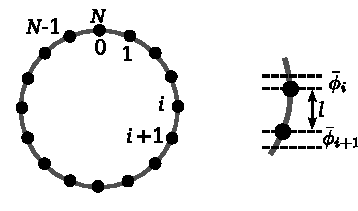
\includegraphics{cuerda} %noinstiki
  \caption{Modelo Cuerda} %noinstiki
  \label{fig:1string} %noinstiki
\end{figure} %noinstiki<div id="fig:1string">Figura cuerda: Modelo cuerda</div>
%noinstiki![cuerda](http://gfif.udea.edu.co/figfs/cuerda.png)
%noinstiki
De acuerdo a la figura 
\ref{fig:1string}, %noinstiki([cuerda](#fig:1string)),
si $\bar{\phi_i}=\bar{\phi}(z_i,t)$ es el
desplazamiento de la $i$--esima masa desde su posici\'on de equilibrio,
entonces el Lagrangiano del sistema de $N$ particulas y resortes es:
\begin{align}
  \label{eq:1strLsum} %noinstiki
  L&=\frac{1}{2}m\sum_{i=0}^{N-1}
  \left(
\frac{\partial\bar\phi_i}{\partial t}
  \right)^2-\frac{1}{2}k\sum_{i=0}^{N-1}
  \left(
\bar\phi_{i+1}-\bar\phi_{i}
  \right)^2,\\
  \label{eq:1strLsumdot} 
&=\frac{1}{2}m\sum_{i=0}^{N-1}
  \left(
    \dot{\bar{\phi_i}}
  \right)^2-\frac{1}{2}k\sum_{i=0}^{N-1}
  \left(
\bar\phi_{i+1}-\bar\phi_{i}
  \right)^2.
\end{align}
Si $\mu$ es la densidad de la cuerda, $T$ la tensi\'on y $v$ la velocidad, entonces
\begin{align}
  \label{eq:micromacro}
  \mu&=\frac{m}{l}\nonumber\\
  T&=kl\\
  v^2&=\frac{T}{\mu}.\nonumber
\end{align}
(\ref{eq:micromacro})
En el l\'\i mite $l\to0$ y $N\to\infty$, tenemos
\begin{equation}
  \label{eq:barf}
  \bar\phi_i=\bar\phi(z_i,t)\to\bar\phi(z,t),
\end{equation}
que representa la funci\'on de campo del desplazamiento de una masa
infinitesimal de su posici\'on de equilibrio. Entonces
\begin{align}
L&=\frac{1}{2}\sum_{i=0}^{N-1}\frac{m}{l}l
  \left(
    \dot{\bar{\phi_i}}
  \right)^2-\frac{1}{2}\sum_{i=0}^{N-1}(k l) l
  \left(
\frac{\bar\phi_{i+1}-\bar\phi_{i}}{l}
  \right)^2.\nonumber\\
&=\frac{1}{2}\sum_{i=0}^{N-1}\mu
  \left(
    \dot{\bar{\phi_i}}
  \right)^2l-\frac{1}{2}\sum_{i=0}^{N-1}T
  \left(
\frac{\bar\phi_{i+1}-\bar\phi_{i}}{l}
  \right)^2l.
\label{eq:1strLsumm}
\end{align}
En el l\'\i mite continuo $\sum(\cdots)\,l\to\int(\cdots)\,dz$, entonces 
\begin{equation}
\label{eq:238}
  L=\int_0^L\frac{1}{2}
\left[
  \mu\left(\frac{\partial\bar\phi}{\partial t}\right)^2- T\left(\frac{\partial\bar\phi}{\partial z}\right)^2
\right]dz=\int_0^L\mathcal{L}dz,
\end{equation}
con
\begin{equation}
  \label{eq:call1}
  \mathcal{L}=\frac{1}{2}
\left[
  \mu\left(\frac{\partial\bar\phi}{\partial t}\right)^2- T\left(\frac{\partial\bar\phi}{\partial z}\right)^2
\right],
\end{equation}
y
\begin{equation}
  \label{eq:Scall}
  S=\int\mathcal{L}\,dtdz.
\end{equation}
Definiendo
\begin{equation}
  \label{eq:barff}
  \phi=\sqrt{T}\bar\phi,
\end{equation}
tenemos
\begin{align}
  \label{eq:call2}
  \mathcal{L}(\partial\phi/\partial t,\partial\phi/\partial z)=&
\frac{1}{2}
\left[
  \frac{\mu}{T}\left(\frac{\partial\phi}{\partial t}\right)^2- \frac{T}{T}\left(\frac{\partial\phi}{\partial z}\right)^2
\right]\nonumber\\
=&\frac{1}{2}
\left[
  \frac{1}{v^2}\left(\frac{\partial\phi}{\partial t}\right)^2-\left(\frac{\partial\phi}{\partial z}\right)^2
\right],
\end{align}
Note que:
\begin{align}
  \label{eq:dcalt}
  \frac{\partial}{\partial t}
  \left[
    \frac{\partial\mathcal{L}}{\partial
      (\partial\phi/\partial t)}
  \right]&=    \frac{1}{v^2}\frac{\partial^2\phi}{\partial t^2}\\
  \label{eq:dcalz} %noinstiki
  \frac{\partial}{\partial z}
  \left[
    \frac{\partial\mathcal{L}}{\partial
      (\partial\phi/\partial z)}
  \right]&= -\frac{\partial^2\phi}{\partial z^2}
\end{align}


Si en la ec.~\eqref{eq:1strLsumdot}, tomamos como coordenadas
generalizadas las $N$ $\dot{\bar{\phi_i}}$ y $\bar\phi_i$, entonces, podemos
obtener las ecuaciones de movimiento a partir de las ecuaciones de
Euler-Lagrange \eqref{eq:eel}:
\begin{equation}
  \label{eq:eelfi}
   \frac{d}{dt} \left ( \frac{\partial L}{\partial\dot{\bar{\phi_i}}} \right ) -
   \frac{\partial L}{\partial \bar\phi_i} = 0,
\qquad \text{$i=0$ hasta $N-1$}.
\end{equation}
En el l\'\i mite $l\to0$ y $N\to\infty$, y usando las ecs.~\eqref{eq:dcalt} 
y \eqref{eq:dcalz}, %noinstiki
\begin{align}
  \label{eq:emov1}
  \frac{d}{dt} \left( \frac{\partial L}{\partial\dot{\bar{\phi_i}}} \right)
  &=\frac{d}{dt} \left( m\dot{\bar{\phi_i}} \right)
= m\frac{\partial^2\bar{\phi_i}}{\partial t^2} \nonumber\\
&= T l\left(\frac{\mu}{T}\frac{\partial^2\bar{\phi_i}}{\partial t^2} \right)\nonumber\\
  &\to
  l\sqrt{T}
  \left(
    \frac{1}{v^2}\frac{\partial^2\phi}{\partial t^2}
  \right)\\
  \label{eq:eecalt} %noinstiki
  &=l\sqrt{T}\frac{\partial}{\partial t}
  \left[
    \frac{\partial\mathcal{L}}{\partial
      (\partial\phi/\partial t)}
  \right].
\end{align}
Para el segundo t\'ermino de la ec.~(\ref{eq:eelfi}) n\'otese que
\begin{align}
- \sum_{i=0}^{N-1}\left(\bar\phi_{i+1}-\bar\phi_{i}\right)^2= 
 &-\left(\bar\phi_{1}-\bar\phi_{0}\right)^2-\left(\bar\phi_{2}-\bar\phi_{1}\right)^2-\cdots
-\left(\bar\phi_{(i-1)+1}-\bar\phi_{i-1}\right)^2-\left(\bar\phi_{i+1}-\bar\phi_{i}\right)^2-\cdots\nonumber\\
 =&-\left(\bar\phi_{1}-\bar\phi_{0}\right)^2-\left(\bar\phi_{2}-\bar\phi_{1}\right)^2-\cdots
 -\left(\bar\phi_{i}-\bar\phi_{i-1}\right)^2-\left(\bar\phi_{i+1}-\bar\phi_{i}\right)^2-\cdots\nonumber\\
\end{align}
Entonces
\begin{align}
-\frac{\partial}{\partial\bar\phi_i}  \sum_{i=0}^{N-1}\left(\bar\phi_{i+1}-\bar\phi_{i}\right)^2
=&-2\left(\bar\phi_{i}-\bar\phi_{i-1}\right)-2\left(\bar\phi_{i+1}-\bar\phi_{i}\right)\times(-1)\nonumber\\
=&2l\left[\frac{\bar\phi_{i+1}-\bar\phi_{i}}{l}-\frac{\bar\phi_{i}-\bar\phi_{i-1}}{l}\right].\nonumber
\end{align}
Si $\bar{z}_i$ es el punto medio del intervalo entre $z_{i-1}$ y $z_i$, entonces en el l\'\i mite de $l\to0$,
\begin{align}
  -\frac{\partial}{\partial\bar\phi_i}  \sum_{i=0}^{N-1}\left(\bar\phi_{i+1}-\bar\phi_{i}\right)^2
  =&2l^2\left\{\frac{[\bar\phi(z_{i+1},t)-\bar\phi(z_{i},t)]/l}{l}-\frac{[\bar\phi(z_{i},t)-\bar\phi(z_{i-1},t)]/l}{l}\right\}\nonumber\\
&2l^2\left[\frac{\partial\bar\phi(\bar z_{i+1},t)/\partial z}{l}-\frac{\partial\bar\phi(\bar z_{i},t)/\partial z}{l}\right]\nonumber\\
  =&2l^2\frac{\partial^2\bar\phi}{\partial z^2}\nonumber\\
  \label{eq:129}
  \to&\frac{2l^2}{\sqrt{T}}\frac{\partial^2\phi}{\partial z^2}.
\end{align}
Usando las ecs.~(\ref{eq:129}) (\ref{eq:micromacro}), tenemos

\begin{align}
  \label{eq:emov2}
  \frac{\partial L}{\partial\bar{\phi_i}}
&=\frac{1}{2}k
\left[-\frac{\partial}{\partial\bar{\phi_i}}\sum_{i=0}^{N-1}\left(\bar\phi_{i+1}-\bar\phi_{i}\right)^2\right]
\nonumber\\
&\to\frac{1}{2}k\left(\frac{2l^2}{\sqrt{T}}\right)\frac{\partial^2\phi}{\partial z^2}
\nonumber\\
&\to  l\sqrt{T}
      \frac{\partial^2\phi}{\partial z^2}\\
  \label{eq:eecalz}
  &=-l\sqrt{T}\frac{\partial}{\partial z}
  \left[
    \frac{\partial\mathcal{L}}{\partial
      (\partial\phi/\partial z)}
  \right].
\end{align}
De las ecuaciones \eqref{eq:emov1} y \eqref{eq:emov2}, obtenemos la
ecuaci\'on de movimiento para el campo $\phi(z,t)$:
\begin{equation}
  \label{eq:econda1}
    \frac{1}{v^2}\frac{\partial^2\phi}{\partial t^2}-\frac{\partial^2\phi}{\partial z^2}=0,
\end{equation}
que corresponde a la ecuaci\'on de onda en una dimensi\'on. En tres
dimensiones obtendr\'\i amos:
\begin{equation}
  \label{eq:econda3}
    \frac{1}{v^2}\frac{\partial^2\phi}{\partial t^2}-\nabla^2\phi=0.
\end{equation}
De otro lado, de las ecuaciones 
\eqref{eq:eecalt} %noinstiki\eqref{eq:emov1}
y \eqref{eq:eecalz}, %noinstiki\eqref{eq:emov2},
obtenemos las ecuaciones de Euler-Lagrange para la densidad Lagrangiana
\begin{equation}
  \label{eq:eelcalls1}
\frac{\partial}{\partial t}
  \left[
    \frac{\partial\mathcal{L}}{\partial
      (\partial\phi/\partial t)}
  \right]+  \frac{\partial}{\partial z}
  \left[
    \frac{\partial\mathcal{L}}{\partial
      (\partial\phi/\partial z)}
  \right]=0.
\end{equation}
En tres dimensiones:
\begin{equation}
  \label{eq:eelcalls1m}
\frac{\partial}{\partial t}
  \left[
    \frac{\partial\mathcal{L}}{\partial
      (\partial\phi/\partial t)}
  \right]+\frac{\partial}{\partial x}
  \left[
    \frac{\partial\mathcal{L}}{\partial
      (\partial\phi/\partial x)}
  \right]+\frac{\partial}{\partial y}
  \left[
    \frac{\partial\mathcal{L}}{\partial
      (\partial\phi/\partial y)}
  \right]+\frac{\partial}{\partial z}
  \left[
    \frac{\partial\mathcal{L}}{\partial
      (\partial\phi/\partial z)}
  \right]=0.
\end{equation}
Definiendo
\begin{equation}
  \label{eq:xmu}
  x^\mu=(x^0,x^i)=(x^0,x^1,x^2,x^3)=(t,x,y,z) \qquad \mu=0,1,2,3,\quad i=1,2,3\,,
\end{equation}
podemos expresar las ecuaciones de Euler-Lagrange que satisface
$\mathcal{L}(\partial\phi/\partial x^\mu)$, como
\begin{align*}
 \sum_\mu\frac{\partial}{\partial x^\mu}
  \left[
    \frac{\partial\mathcal{L}}{\partial
      (\partial\phi/\partial x^\mu)}
  \right]&=0\\
 \frac{\partial}{\partial x^\mu}
  \left[
    \frac{\partial\mathcal{L}}{\partial
      (\partial\phi/\partial x^\mu)}
  \right]&=0,
\end{align*}
donde, en la \'ultima ecuaci\'on se ha usado la convenci\'on de suma sobre
\'\i ndices repetidos. 

Si la densidad Lagrangiana depende tambi\'en directamente de $\phi$,
$\mathcal{L}(\partial\phi/\partial x^\mu,\phi)$, entonces la ecuaci\'on de Euler-Lagrange para
las coordenadas generalizadas  $\partial\phi/\partial x^\mu$ y $\phi$, es
\begin{equation}
\label{eq:eelcallf}
 \frac{\partial}{\partial x^\mu}
  \left[
    \frac{\partial\mathcal{L}}{\partial
      (\partial\phi/\partial x^\mu)}
  \right]-\frac{\partial\mathcal{L}}{\partial\phi}=0.
\end{equation}
\'Esta \'ultima ecuaci\'on se deducir\'a usando m\'etodos variacionales en la
siguiente secci\'on.

\section{Principio de M\'\i nima Acci\'on para $\mathcal{L}$}
\label{sec:principio-de-minima-call}
\subsection{Ecuaciones de Euler-Lagrange}

Definamos
\begin{equation}
  \label{eq:dmu}
  \partial_\mu=\frac{\partial}{\partial x^\mu},
  \end{equation}
En tres dimensiones, la acci\'on de la ec.~\eqref{eq:Scall}, queda
\begin{equation}
  \label{eq:Scall3d}
  S[\phi,\partial_\mu\phi]=\int_{R}d^4x\mathcal{L}(\phi,\partial_\mu\phi)
\end{equation}
donde $d^4x=d t\,d x\, d y\,d z$.  Considere primero una variaci\'on s\'olo de
los campos, tal que ($x=x^\mu)$
\begin{equation}
  \label{eq:deltaphi}
  \delta\phi(x)=\phi'(x)-\phi(x)
\end{equation}
De otro lado, con $\delta x=x'-x$, la expansi\'on de Taylor para $f(x+\delta x)$ es
\begin{equation}
  f(x+\delta x)=f(x)+\frac{\partial f}{\partial x}\delta x+\cdots 
\end{equation}
Para $\mathcal{L}$, tenemos de la ec.~\eqref{eq:deltaphi}
\begin{align}
  \mathcal{L}(\phi',\partial_\mu\phi')&=\mathcal{L}(\phi+\delta\phi,\partial_\mu\phi+\partial_\mu(\delta\phi))\nonumber\\
  &=\mathcal{L}+\frac{\partial\mathcal{L}}{\partial\phi}\delta\phi+\frac{\partial\mathcal{L}}{\partial(\partial_\mu\phi)}\partial_\mu(\delta\phi)
\end{align}
Entonces, de imponer que $\delta S=0$, tenemos
\begin{align}
  \delta S&=S'-S=\int_{R}d^4x\,\mathcal{L}(\phi',\partial_\mu\phi')-\int_{R}d^4x\,\mathcal{L}(\phi,\partial_\mu\phi)\nonumber\\
&=\int_{R}d^4x\,
\left[
\frac{\partial\mathcal{L}}{\partial\phi}\delta\phi+\frac{\partial\mathcal{L}}{\partial(\partial_\mu\phi)}\partial_\mu(\delta\phi)
\right]\nonumber\\
 &=\int_{R}d^4x\,
  \left\{ 
    \frac{\partial\mathcal{L}}{\partial\phi}-\left[\partial_\mu\left(
      \frac{\partial\mathcal{L}}{\partial(\partial_\mu\phi)}
    \right)\right]
  \right\}\delta\phi+\int_{R}d^4x\,
    \partial_\mu\left[
      \frac{\partial\mathcal{L}}{\partial(\partial_\mu\phi)}\delta\phi
    \right]\nonumber\\
\label{eq:1}
\delta S&=\int_{R}d^4x\,
  \left\{ 
    \frac{\partial\mathcal{L}}{\partial\phi}-    
    \left[\partial_\mu\left(
      \frac{\partial\mathcal{L}}{\partial(\partial_\mu\phi)}
    \right)\right]
  \right\}\delta\phi+\int_{\sigma}\left[
      \frac{\partial\mathcal{L}}{\partial(\partial_\mu\phi)}\delta\phi
    \right]\,d\sigma_\mu=0.
\end{align}
Donde hemos aplicado el Teorema de Gauss
\begin{equation}
\int_V\boldsymbol{\nabla}\cdot\mathbf{A}\,d^3x=
 \int_S\mathbf{A}\cdot d\mathbf{S}\,
\end{equation}
generalizado a cuatro dimensiones. Como la variaci\'on de $\delta\phi$ es cero sobre la hipersuperficie $\sigma$ resulta 
\begin{equation}
  \int_{R}d^4x\,
  \left\{ 
    \frac{\partial\mathcal{L}}{\partial\phi}-
   \left[\partial_\mu\left(
      \frac{\partial\mathcal{L}}{\partial(\partial_\mu\phi)}
    \right)\right]
  \right\}\delta\phi=0.
\end{equation}
Como $\delta\phi$ es cualquier posible variaci\'on entre las fronteras de la hipersuperficie, el integrando debe anularse y resultan las ecuaciones de Euler-Lagrange:
\begin{equation}
\label{eq:eelcallfmu}
 \partial_\mu
  \left[
    \frac{\partial\mathcal{L}}{\partial
      (\partial_\mu\phi)}
  \right]-\frac{\partial\mathcal{L}}{\partial\phi}=0.
\end{equation}
La densidad Lagrangiana
\begin{align}
  \mathcal{L}'=\mathcal{L}+\partial_\mu(\eta(x))
\end{align}
donde $\eta(x)$ es cualquier funci\'on de los campos de la densidad Lagrangiana original, da lugar a la Acci\'on
\begin{align}
  S'=\int_{R}d^4x\,\mathcal{L}'=&\int_{R}d^4x\,\mathcal{L}+\int_R d^4x\,\partial_\mu\eta\nonumber\\
  =&\int_{R}d^4x\,\mathcal{L}+\int_\sigma \eta d\sigma^\mu\nonumber\\
  =&S\,,
\end{align}
para una hipersuperficie suficientemente grande. De modo que dos densidades lagrangianas que difieran solo en derivadas totales dan lugar a la misma Acci\'on.

Usando el principio de m\'\i nima acci\'on en t\'erminos del campo $\phi$, tenemos que para la densidad Lagrangiana~\eqref{eq:call2}
\begin{align}
  \mathcal{L}=&\frac{1}{2}  \left[
  \frac{1}{v^2}\left(\frac{\partial\phi}{\partial t}\right)^2-\left(\frac{\partial\phi}{\partial z}\right)^2
\right],
\end{align}
las ecuaciones de Euler-Lagrange~\eqref{eq:eelcallfmu}
\begin{align}
  \partial_0\left[\frac{\partial\mathcal{L}}{\partial(\partial_0\phi)}\right]+
\partial_3\left[\frac{\partial\mathcal{L}}{\partial(\partial_3\phi)}\right]
-\frac{\partial\mathcal{L}}{\partial\phi}=&0\nonumber\\
  \frac{\partial}{\partial t}\left[\frac{\partial\mathcal{L}}{\partial(\partial\phi/\partial t)}\right]+
\frac{\partial}{\partial z}\left[\frac{\partial\mathcal{L}}{\partial(\partial\phi/\partial z)}\right]
=&0\nonumber\\
 \frac{1}{v^2}\frac{\partial}{\partial t}\left[\frac{\partial\phi}{\partial t}\right]
-\frac{\partial}{\partial z}\left[\frac{\partial\phi}{\partial z}\right]=&0\nonumber\\
 \frac{1}{v^2}\frac{\partial^2\phi}{\partial t^2}-\frac{\partial^2\phi}{\partial z^2}=&0\,,
\end{align}
que corresponde a la ec.~\eqref{eq:econda1}.

Generalizando a tres dimensiones vemos que la ecuaci\'on para una onda propagandose a una velocidad $v$, eq.~\eqref{eq:econda3},  
\begin{equation}
     \frac{1}{v^2}\frac{\partial^2\phi}{\partial t^2}-\nabla^2\phi=0\,,
\end{equation}
proviene de una densidad Lagrangiana (hasta derivadas totales)
\begin{align}
    \label{eq:ls3d}
    \mathcal{L}=&\frac{1}{2}\left[
  \left(
\frac{1}{v^2}\frac{\partial\phi}{\partial t}
  \right)^2-\boldsymbol{\nabla}\phi\cdot\boldsymbol{\nabla}\phi \right]\nonumber\\
    =&\frac{1}{2}\left[
      \frac{1}{v^2}{\partial_0\phi}\,{\partial_0\phi}-\sum_i{\partial_i\phi}\,{\partial_i\phi}
   \right]\,.
\end{align}
\subsection{Teorema de Noether para simetr\'\i as internas}
Para un campo complejo la ec.~(\ref{eq:Scall3d}) se generaliza a
\begin{equation}
  S[\phi,\phi^*,\partial_\mu\phi,\partial_\mu\phi^*]=\int_{R}d^4x\,\mathcal{L}(\phi,\phi^*,\partial_\mu\phi,\partial_\mu\phi^*)
\end{equation}
Usando el mismo procedimiento, se obtiene
\begin{align}
  \label{eq:130}
   \delta S=&\int_{R}d^4x\,
  \left\{ 
    \frac{\partial\mathcal{L}}{\partial\phi}-
  \left[\partial_\mu\left(
      \frac{\partial\mathcal{L}}{\partial(\partial_\mu\phi)}
    \right)\right]
  \right\}\delta\phi
+\int_{R}d^4x\,
  \left\{ 
    \frac{\partial\mathcal{L}}{\partial\phi^*}-
  \left[\partial_\mu\left(
      \frac{\partial\mathcal{L}}{\partial(\partial_\mu\phi^*)}
    \right)\right]
  \right\}\delta\phi^*\nonumber\\
&+\int_{R}d^4x\,
    \partial_\mu\left[
      \frac{\partial\mathcal{L}}{\partial(\partial_\mu\phi)}\delta\phi+
      \delta\phi^*\frac{\partial\mathcal{L}}{\partial(\partial_\mu\phi^*)}
    \right]=0.
\end{align}
Usando de nuevo el Teorema de Gauss resultan las ecuaciones de Euler Lagrange para $\phi$ y $\phi^*$
\begin{equation}
\label{eq:132}
  \partial_\mu
  \left[
    \frac{\partial\mathcal{L}}{\partial
      (\partial_\mu\phi)}
  \right]-\frac{\partial\mathcal{L}}{\partial\phi}=0, \qquad
  \partial_\mu
  \left[
    \frac{\partial\mathcal{L}}{\partial
      (\partial_\mu\phi^*)}
  \right]-\frac{\partial\mathcal{L}}{\partial\phi^*}=0.
\end{equation}
De otro lado, si asumimos que $\phi$ y $\phi^*$ satisfacen las ecuaciones de Euler--Lagrange, en lugar de asumir que $\delta\phi$ y $\delta\phi^*$ se anulan sobre la hipersuperficie, los dos primeros t\'erminos de la ec.~(\ref{eq:130}) se anulan y tendremos que para que $\delta S=0$:
\begin{equation}
  \label{eq:jmu}
  \int_{R}d^4x\,(\partial_\mu J^\mu)=0,
\end{equation}
donde,
\begin{equation}
  \label{eq:jmuphi}
 J^\mu= \left[
      \frac{\partial\mathcal{L}}{\partial(\partial_\mu\phi)}
    \right]\delta\phi+\delta\phi^*\left[
      \frac{\partial\mathcal{L}}{\partial(\partial_\mu\phi^*)}
    \right]
\end{equation}
Entonces $J^\mu$ satisface la ecuaci\'on de continuidad:
\begin{align}
  \label{eq:conti}
  \partial_\mu J^\mu&=0\\
\frac{\partial J^0}{\partial t}+\boldsymbol{\nabla}\cdot\mathbf{J}&=0
\end{align}
Integrando con respecto al volumen
\begin{align}
  &\int_V\frac{\partial J^0}{\partial t}\,d^3x+\int_V\boldsymbol{\nabla}\cdot\mathbf{J}\,d^3x=0,\nonumber\\
  &\int_V\frac{\partial J^0}{\partial t}\,d^3x+\int_S\mathbf{J}\cdot d\mathbf{S}=0,
\end{align}
Escogiendo una superficie suficientemente grande que abarque toda la fuente de densidad $\rho=J^0$, de la corriente $\mathbf{J}$, el segundo integrando es cero y
\begin{equation}
  \frac{d}{dt}\int_V\rho\,d^3x=0.
\end{equation}
Este resultado es conocido como Teorema de Noether. \'Este establece que para
toda transformaci\'on continua del tipo \eqref{eq:deltaphi}, debe
existir una cantidad conservada, $dQ/dt=0$, que en este caso corresponde a
\begin{equation}
  \label{eq:qcons}
  Q=\int_V \rho\,d^3x.
\end{equation}
\subsection{Teorema de Noether para simetr\'\i as externas}
Para el caso de una simetr\'\i a externas, por ejemplo la correspondiente a una traslaci\'on espacio--temporal
\begin{align}
  x^\mu\to{x'}^\mu=&x^\mu+\delta a^\mu\nonumber\\
  \delta x^\mu=&\delta a^\mu
\end{align}

tenemos
\begin{align}
  \phi'(x')&=\phi'(x+\delta a)\\
  &\approx\phi'(x)+\frac{\partial\phi'(x)}{\partial x^\mu}\delta a^\mu\\
  &=[\phi(x)+\delta\phi(x)]+\frac{\partial}{\partial x^\mu}[\phi(x)+\delta\phi(x)]\delta a^\mu\\
  &\approx\phi(x)+\delta\phi(x)+\frac{\partial\phi(x)}{\partial x^\mu}\delta a^\mu,
\end{align}
donde, por simplicidad, $\phi$ es de nuevo un campo real. Entonces,
\begin{equation}
  \label{eq:Deltaf}
  \Delta\phi(x)\equiv\phi'(x')-\phi(x)=\delta\phi(x)+\frac{\partial\phi(x)}{\partial x^\mu}\delta a^\mu.
\end{equation}
Para una traslaci\'on, $\Delta\phi(x)=0$, ver figura 
\ref{fig:trasla}. %noinstiki([trasla](#fig:trasla)).
De modo que
\begin{equation}
  \label{eq:dmuxmu}
  \delta\phi=-(\partial_\mu\phi)\delta a^\mu,
\end{equation}
y la transformaci\'on del campo $\phi$ como consecuencia de la traslaci\'on es
\begin{align}
  \phi(x)\to\phi'(x)=\phi(x)-\delta\phi(x)=\phi(x)+(\partial_\mu\phi(x))\delta a^\mu\,.
\end{align}
%noinstiki

\begin{figure} %noinstiki
  \centering %noinstiki
  \includegraphics{trasla} %noinstiki
  \caption{Traslaci\'on de funci\'on y coordenadas en una dimensi\'on: $\phi(x)=\phi'(x')$ } %noinstiki
  \label{fig:trasla} %noinstiki
\end{figure} %noinstiki<div id="fig:trasla">Figura trasla:Traslaci\'on de funci\'on y coordenadas $\phi(x)=\phi(x')$ </div>
%noinstiki![trasla](http://gfif.udea.edu.co/figfs/trasla.png)
%noinstiki
Si $a^\mu$ es constante (un an\'alisis m\'as general es hecho en \cite{r})
\begin{equation}
  d^4x'=d^4x
\end{equation}
En este caso, asumiendo que el campo satisface las ecuaciones de
Euler-Lagrange y usando la ec.~\eqref{eq:dmuxmu} y (\ref{eq:eelcallfmu}) tenemos
\begin{align}
  \delta S&=\int_{R}d^4x\,\mathcal{L}(\phi',\partial_\mu\phi',x')-\int_{R}d^4x\,\mathcal{L}(\phi(x),\partial_\mu\phi(x),x)\nonumber\\
  &=\int_{R}d^4x\,\mathcal{L}(\phi+\delta\phi,\partial_\mu\phi+\partial_\mu(\delta\phi),x+\delta a)-\int_{R}d^4x\,\mathcal{L}\nonumber\\
  &\approx\int_{R}d^4x\,
  \left[\mathcal{L}+
    \frac{\partial\mathcal{L}}{\partial\phi}\delta\phi+\frac{\partial\mathcal{L}}{\partial(\partial_\mu\phi)}\partial_\mu(\delta\phi)+
    (\partial_\mu\mathcal{L})\delta a^\mu\right]-\int_{R}d^4x\,\mathcal{L}\nonumber\\
  &=\int_{R}d^4x\,
  \left[
    \frac{\partial\mathcal{L}}{\partial\phi}\delta\phi+\frac{\partial\mathcal{L}}{\partial(\partial_\mu\phi)}\partial_\mu(\delta\phi)+
    (\partial_\mu\mathcal{L})\delta a^\mu\right]\nonumber\\
  &=\int_{R}d^4x\,
  \left\{ 
    \left[\partial_\mu\left(\frac{\partial\mathcal{L}}{\partial(\partial_\mu\phi)}
    \right)\right]\delta\phi+\frac{\partial\mathcal{L}}{\partial(\partial_\mu\phi)}\partial_\mu(\delta\phi)+
    (\partial_\mu\mathcal{L})\delta a^\mu\right\}\nonumber\\
  &=\int_{R}d^4x\left\{ 
    \partial_\mu\left[\frac{\partial\mathcal{L}}{\partial(\partial_\mu\phi)}\delta\phi\right]
  +(\partial_\mu\mathcal{L})\delta a^\mu\right\}\nonumber\\
  &=\int_{R}d^4x\,
    \partial_\mu\left[
      -\frac{\partial\mathcal{L}}{\partial(\partial_\mu\phi)}(\partial_\nu\phi)
      +\delta^\mu_\nu\mathcal{L}
    \right]\delta a^\nu\nonumber\\
    \label{eq:2}
  &=\int_{R}d^4x\,
  \left(
    \partial_\mu T^\mu_\nu
  \right)\delta a^\nu=0.
\end{align}
Y por consiguiente
\begin{equation}
  \label{eq:131}
  \partial_\mu T^\mu_\nu=0,
\end{equation}
donde
\begin{equation}
  \label{eq:tmunu}
    T^\mu_\nu=\frac{\partial\mathcal{L}}{\partial(\partial_\mu\phi)}(\partial_\nu\phi)
      -\delta^\mu_\nu\mathcal{L}
\end{equation}
El tensor $T^\mu_\nu$ proviene de asumir la homogeneidad del espacio y el tiempo y es llamado el tensor de momentum--energ\'\i a. 
La densidad Hamiltonina se obtiene de $T^0_0$
\begin{align}
  \label{eq:3}
\mathcal{H}&=T^0_0=\frac{\partial\mathcal{L}}{\partial\dot{\phi}}\dot{\phi}
      -\mathcal{L}\\
      &=\pi(x)\frac{\partial\phi(x)}{\partial t}-\mathcal{L}.
\end{align}
Comparando con la expresi\'on correspondiente en la formulaci\'on
Lagrangiana de la Mec\'anica Cl\'asica, tenemos que si $\phi(x)$ es la
variable can\'onica, la variable can\'onica conjugada es $\pi(x)$
\begin{equation}
  \label{eq:4}
  \pi(x)=\frac{\partial\mathcal{L}}{\partial(\partial\phi(x)/\partial t)}.
\end{equation}
El teorema de Noether en este caso establece que la invarianza de la Acci\'on bajo traslaciones temporales da lugar a la ecuaci\'on de continuidad (\ref{eq:131}) para $\nu=0$
\begin{align}
\label{eq:122}
  \partial_\mu T^\mu_0=0
\end{align}
cuya carga conservada corresponde a la energ\'\i a
\begin{align}
  H=\int_V d^3x\, T^0_0=\int_V d^3x\,\mathcal{H}.
\end{align}
De igual forma la invarianza bajo traslaciones espaciales de lugar a ecuaciones de continuidad para cada componente $\nu=i$
 ($i=1,2,3$)
 \begin{align}
   \label{eq:235}
   \partial_\mu T^\mu_i=0,
 \end{align}
cuyas densidad de cargas conservadas, $T^0_i$, que en forma vectorial escribiremos como $\mathbf{T}^0$, dan lugar a la conservaci\'on del momentum
\begin{align}
  \mathbf{P}=\int_V d^3x\,\mathbf{T}^0\,.
\end{align}
Generalizando a un campo complejo
\begin{equation}
  \label{eq:138}
     T^\mu_\nu=\frac{\partial\mathcal{L}}{\partial(\partial_\mu\phi)}(\partial_\nu\phi)+(\partial_\nu\phi^*)\frac{\partial\mathcal{L}}{\partial(\partial_\mu\phi^*)}
      -\delta^\mu_\nu\mathcal{L}
\end{equation}

\section{Aplicaci\'on a Mec\'anica Cu\'antica}
\label{sec:aplic-mecan-cuant}

Haciendo $\hbar=1$, el Lagrangiano que da lugar a la ecuaci\'on de Schr\"odinger es
\begin{align}
\label{eq:5}
  \mathcal{L}(\psi,\psi^*,\partial_\mu\psi,\partial_\mu\psi^*)&=\frac{1}{2m}\boldsymbol{\nabla}\psi^*\cdot\boldsymbol{\nabla}\psi-\frac{i}{2}
  \left(
\psi^*\frac{\partial\psi}{\partial t}-\frac{\partial\psi^*}{\partial t}\psi
  \right)+\psi^*V\psi\\
&=\frac{1}{2m}\partial_i\psi^*\partial_i\psi-\frac{i}{2}
  \left(\psi^*\partial_0\psi-\partial_0\psi^*\psi\right)+\psi^*V\psi.\nonumber
\end{align}
Aplicando las ecuaciones de Euler-Lagrange (\ref{eq:132}) para
la funci\'on de onda $\psi^*$ obtenemos la ecuaci\'on de Scr\"odinger con $\hbar=1$:
\begin{equation}
  \label{eq:137}
    0=\partial_\mu\left[\frac{\partial\mathcal{L}}{\partial(\partial_\mu\psi^*)}\right]-\frac{\partial\mathcal{L}}{\partial\psi^*}=
  \partial_0\left[\frac{\partial\mathcal{L}}{\partial(\partial_0\psi^*)}\right]+  
\partial_i\left[\frac{\partial\mathcal{L}}{\partial(\partial_i\psi^*)}\right]-\frac{\partial\mathcal{L}}{\partial\psi^*}.
\end{equation}
Como
\begin{align}
  \label{eq:136}
  &\frac{\partial\mathcal{L}}{\partial(\partial_0\psi)}=-\frac{i}{2}\psi^*&&\frac{\partial\mathcal{L}}{\partial(\partial_0\psi^*)}=\frac{i}{2}\psi\nonumber\\
  &\frac{\partial\mathcal{L}}{\partial(\partial_i\psi)}=\frac{1}{2m}\partial_i\psi^*&&\frac{\partial\mathcal{L}}{\partial(\partial_i\psi^*)}=\frac{1}{2m}\partial_i\psi\\
  &\frac{\partial\mathcal{L}}{\partial\psi}=\frac{i}{2}\partial_0\psi^*+\psi^*V&&\frac{\partial\mathcal{L}}{\partial\psi^*}=-\frac{i}{2}\partial_0\psi+V\psi.\nonumber
\end{align}
Entonces, reemplazando la ec.~(\ref{eq:136}) en la ec.~(\ref{eq:137}), tenemos
\begin{align}
 0=\partial_\mu\left[\frac{\partial\mathcal{L}}{\partial(\partial_\mu\psi^*)}\right]-\frac{\partial\mathcal{L}}{\partial\psi^*}
 &=\partial_0\left(\frac{i}{2}\psi\right)+\partial_i\left(\frac{1}{2m}\partial_i\psi\right)
  -\left(-\frac{i}{2}\partial_0\psi+V\psi\right)\nonumber\\
  &=\frac{i}{2}\partial_0\psi+\frac{1}{2m}\partial_i\partial_i\psi+\frac{i}{2}\partial_0\psi-V\psi.
\end{align}

Que puede escribirse como
\begin{equation}
  \label{eq:133}
  i\frac{\partial}{\partial t}\psi=
  \left(
    -\frac{1}{2m}\nabla^2+V
  \right)\psi.
\end{equation}

El Lagrangiano en ec~(\ref{eq:5}), y por consiguiente la Acci\'on, es invariante bajo una transformaci\'on de fase
\begin{equation}
  \label{eq:6}
  \psi\to\psi'=e^{i\theta}\psi.
\end{equation}
Por consiguiente, de acuerdo al Teorema de Noether, debe existir una cantidad conservada. La corriente conservada se obtine de la ec.~(\ref{eq:jmuphi}). Para los campos $\psi$ y $\psi^*$, tenemos
\begin{align}
  \delta\psi=\psi'-\psi=(e^{i\theta}-1)\psi&\approx i\theta\psi\\
  \delta\psi^*&\approx-i\theta\psi.
\end{align}
Usando adem\'as la ec.~(\ref{eq:136}) en la definici\'on de $J^0$ dada por la ec.~(\ref{eq:jmuphi}), tenemos
\begin{align}
  \label{eq:135}
  J^0&=\left[\frac{\partial\mathcal{L}}{\partial(\partial_0\psi)}\right]\delta\psi
  +\delta\psi^*\left[\frac{\partial\mathcal{L}}{\partial(\partial_0\psi^*)}\right]\nonumber\\
  &=-\frac{i}{2}\psi^*(i\theta\psi)+(-i\theta\psi^*)\frac{i}{2}\psi\nonumber\\
  &=\theta\psi^*\psi,
\end{align}
y
\begin{align}
  \label{eq:134}
  J^i&=\left[\frac{\partial\mathcal{L}}{\partial(\partial_i\psi)}\right]\delta\psi
  +\delta\psi^*\left[\frac{\partial\mathcal{L}}{\partial(\partial_i\psi^*)}\right]\nonumber\\
  &=\frac{1}{2m}\partial_i\psi^*(i\theta\psi)+(-i\theta\psi^*)\frac{1}{2m}\partial_i\psi\nonumber\\
  &=\frac{i\theta}{2m}\left(\partial_i\psi^*\psi-\psi^*\partial_i\psi \right).
\end{align}
Entonces, normalizando apropiadamente la corriente escogiendo $\theta=1$, tenemos
\begin{align}
  \label{eq:7}
  J^0&=\psi^*\psi\\
  \mathbf{J}&=\frac{i}{2m}
  \left(
    \psi\boldsymbol{\nabla}\psi^*-\psi^*\boldsymbol{\nabla}\psi
  \right).
\end{align}
De acuerdo a la ec.~(\ref{eq:7}), la cantidad conservada corresponde a la probabilidad de la funci\'on de onda y normalizando apropiadamente la ec.~(\ref{eq:qcons})
\begin{equation}
  \label{eq:57}
Q_\rho=  \int_V \psi^*\psi \,d^3x=1.
\end{equation}


En cuanto a las simetr\'\i as externas, tenemos de la ec.~(\ref{eq:tmunu}) que
da lugar a las ecuaciones de continuidad (\ref{eq:122})(\ref{eq:235})
\begin{align}
  \partial_\mu T^\mu_0&=0,\nonumber\\
\partial_\mu{T}^\mu_i&=0
\end{align}
Las cargas conservadas se pueden obtener de las densidades de carga
$T^0_0$ y $T^0_i$. 

\subsection{Conservación del moméntum}
Comencemos con las densidades de carga asociadas a
la conservación del moméntum lineal.
Usando  las ecs.~(\ref{eq:136}) en la ec.~(\ref{eq:138})
\begin{align}
  T^0_i=&\frac{\partial\mathcal{L}}{\partial(\partial_0\psi)}(\partial_i\psi)
  +(\partial_i\psi^*)\frac{\partial\mathcal{L}}{\partial(\partial_0\psi^*)}\nonumber\\
  T^0_i=&-\frac{i}{2}\psi^*(\partial_i\psi)+\frac{i}{2}(\partial_i\psi^*)\psi
\end{align}
Entonces, definiendo
\begin{equation}
   \mathbf{T}^0=\frac{i}{2}
  \left(
    \psi\boldsymbol{\nabla}\psi^*-\psi^*\boldsymbol{\nabla}\psi
  \right)
\end{equation}
Procedemos ahora a reemplazar $\psi\boldsymbol{\nabla}\psi^*$ por la
derivada total
\begin{align}
 \mathbf{T}^0&=\frac{i}{2}
  \left[\left( 
    \boldsymbol{\nabla}(\psi^*\psi)-\psi^*\boldsymbol{\nabla}\psi \right)-\psi^*\boldsymbol{\nabla}\psi
  \right]\nonumber\\
&=-i\psi^*\boldsymbol{\nabla}\psi+\frac{i}{2}\boldsymbol{\nabla}(\psi^*\psi)\,.
\end{align}
Integrando en el volumen
\begin{equation}
  \int_V \mathbf{T}^0\, d^3x=-i\int_V \psi^*\boldsymbol{\nabla}\psi\, d^3x+\frac{i}{2}\boldsymbol{\nabla}\int_V\psi^*\psi\,d^3x
\end{equation}
De acuerdo a la ec.~(\ref{eq:57}), la \'ultima integral es una constante y
\begin{align}
  \label{eq:140}
  \int_V \mathbf{T}^0\, d^3x=-i\int_V \psi^*\boldsymbol{\nabla}\psi d^3x\nonumber\\
\langle\widehat{\mathbf{p}}\rangle=\int_V \psi^*\widehat{\mathbf{p}}\psi d^3x
\end{align}
De modo que $\langle\widehat{\mathbf{p}}\rangle$ son las cargas conservadas asociadas al valor esperado el operador de momentum
\begin{equation}
  \widehat{\mathbf{p}}=-i\boldsymbol{\nabla}\,.
\end{equation}
En general, el valor esperado de un operador $ \widehat{\cal O}$, se define en mecánica cuántica como
\begin{align*}
  \langle\widehat{\cal O}\rangle=\int_V d^3x\,\psi^{*}\widehat{\cal O}\psi\,.
\end{align*}

\subsection{Conservación de la energía}
De otro lado
\begin{align}
  T^0_0&=\frac{\partial\mathcal{L}}{\partial(\partial_0\psi)}{\partial_0\psi}+{\partial_0\psi^*}\frac{\partial\mathcal{L}}{\partial(\partial_0\psi^*)}-\mathcal{L}\nonumber\\
  &=-\frac{i}{2}\psi^*\partial_0\psi+\frac{i}{2}\partial_0\psi^*\psi-\frac{1}{2m}\partial_i\psi^*\partial_i\psi+\frac{i}{2}
  \left(\psi^*\partial_0\psi-\partial_0\psi^*\psi\right)-\psi^*V\psi\nonumber\\
  &=-\frac{1}{2m}\partial_i\psi^*\partial_i\psi-\psi^*V\psi
\end{align}
Como las corrientes solo est\'an determinadas hasta un factor de proporcionalidad, definimos
\begin{align}
  \label{eq:139}
   \mathcal{H}&\equiv-T^0_0=\frac{1}{2m}\boldsymbol{\nabla}\psi^*\cdot\boldsymbol{\nabla}\psi+\psi^*V\psi\nonumber\\
   &=\frac{1}{2m}\boldsymbol{\nabla}\cdot(\psi^*\boldsymbol{\nabla}\psi)-\frac{1}{2m}\psi^*\nabla^2\psi+\psi^*V\psi.
\end{align}
Integrando sobre el volumen y usando la ec.~(\ref{eq:140})
\begin{align}
 \int_V\mathcal{H}\,d^3x&=\frac{1}{2m}\int_V\boldsymbol{\nabla}\cdot(\psi^*\boldsymbol{\nabla}\psi)
+\int_V\psi^*\left(-\frac{1}{2m}\nabla^2+V\right)\psi\,d^3x\nonumber\\
&=\frac{1}{2m}\boldsymbol{\nabla}\cdot\int_V(\psi^*\boldsymbol{\nabla}\psi)
+\int_V\psi^*\left(-\frac{1}{2m}\nabla^2+V\right)\psi\,d^3x\nonumber\\
&=\frac{i}{2m}\boldsymbol{\nabla}\cdot\langle\widehat{\mathbf{p}}\rangle
+\int_V\psi^*\left(-\frac{1}{2m}\nabla^2+V\right)\psi\,d^3x\nonumber\\
&=\int_V\psi^*\left(-\frac{1}{2m}\nabla^2+V\right)\psi\,d^3x\,.
\end{align}

Entonces
\begin{align}
\label{eq:141}
H&\equiv \int_V\mathcal{H}\,d^3x=\int_V\psi^*\left(-\frac{1}{2m}\nabla^2+V\right)\psi\,d^3x\nonumber\\
&=\int_{V} d^3x\,\psi^*\widehat{H}\psi=\langle\widehat{H}\rangle.
\end{align}
Que es un resultado bien conocido de la mec\'anica cu\'antica.

Como
\begin{equation}
  \widehat H=\frac{1}{2m}\hat p^2+\widehat V,
\end{equation}
podemos escribir la ec.~(\ref{eq:133}) como
\begin{equation}
  i\frac{\partial}{\partial t}\psi=\widehat H \psi\,.
\end{equation}
Podemos identificar entonces los operadores de energ\'\i a y momentum.
\begin{equation}
  \label{eq:151}
  \widehat H=i\frac{\partial}{\partial t},\qquad \hat{\mathbf{p}}=-i\,\boldsymbol{\nabla}.
\end{equation}

Retornando a la ec.~(\ref{eq:140}), tenemos que para la soluci\'on de part\'\i cula libre de la ecuaci\'on de Schr\"odinger 
\begin{equation}
  \psi=A\,e^{-i\mathbf{k}\cdot\mathbf{x}},
\end{equation}
la condici\'on de normalizaci\'on en ec.~\eqref{eq:57} implica que $|A|^2=1/L^3$, y
\begin{align}
  \int_V \mathbf{T}^0\, d^3x&=\mathbf{k}.
\end{align}

\begin{itemize}
\item[\textbf{Ejercicio:}]  De la ec.~(\ref{eq:141}) obtenega la densidad Hamiltoniana, y usando la ec.~(\ref{eq:3}) encontrar la densidad Lagrangiana~\eqref{eq:5}.
\end{itemize}


\section{Invarianza de fase local del Lagrangiano de  Scrödinger's}

%Trasladar el material de sección 3.4 aquí. 

When we discuss the wave function $\psi(x)$, $x$ represents the point in space at which we want to know the value of the wave function. Since complex numbers are, well, complex, you can't represent them by a position on a simple number line. Instead, the have to be represented by a point in a two--dimensional plot. 

In addition the length of the arrow pointing to the complex number we also need an angle to specify exactly how to draw the arrow pointing to the complex number. The observable is encoded into the length of the arrow representing the value of the complex valued wave function at that point of the space--time. Its angle is unobservable.

The complex number $\psi(x)$ in the Scrödinger equation is just the number whose square is the relative probability of finding the object at that point.

Now, suppose that you arbitrarily decide to make a change of phase of the wave function --to change, at every point in space, the angle $\theta$ of the complex number $\psi$ makes with the real axis. Here is the critical point: Is this change phase is \emph{global}, if the phase that you change the phase angle $\theta$ is the same everywhere in space, the this change of phase will not destroy the delicate and essential balance between the kinetic and potential energy in the Scrödinger equation.

However, in the view implemented by Einstein's relativity, the need to require that quantum--mechanical systems be unaltered only by global changes of phase seemed to be very unnatural. Once you choose the phase of the wave function at one space-time point, the requirement of global phase invariance fixes it at all other space-time points:


  \begin{quote}
\small
    As usually conceived however, this arbitrariness is subject to the following  limitation: once one choose [the phase of the wave function] at one space--time point, one is then not free to make any choices at other space--time points.

It seems that it is not consistent with the localized field concept that underlies the usual physical theories. In the present paper we wish to explore the possibility of requiring all the interactions to be invariant under independent [change of phases] at all space-time points.
  \end{quote}
  \begin{flushright}
    Yang-Mills, \emph{Physical Review}, 1954
  \end{flushright}

This is similar to what happens in electromagnetic theory expressed in terms of scalar and vector potentials. The can be changed by arbitrary functions in a such way that the measured electric and magnetic fields remain invariant. As we will see, this feature is deeply connected with the local conservation of electric charge. 

We start again with the Scrödinger Lagrangian as written in eq.~\eqref{eq:5qft}: but without the interaction term

\begin{align}
  \mathcal{L}(\psi,\psi^*,\partial_\mu\psi,\partial_\mu\psi^*)&=\frac{1}{2m}\boldsymbol{\nabla}\psi^*\cdot\boldsymbol{\nabla}\psi-\frac{i}{2}
  \left(
\psi^*\frac{\partial\psi}{\partial t}-\frac{\partial\psi^*}{\partial t}\psi
  \right)+\cancel{\psi^*V\psi}\\
\mathcal{L}_{\text{free}}&=\frac{1}{2m}\partial_i\psi^*\partial_i\psi-\frac{i}{2}
  \left(\psi^*\partial_0\psi-\partial_0\psi^*\psi\right).\nonumber
\end{align}
This Lagrangian is not invariant under local phase changes of the wave function: 
\begin{align}
  \partial_\mu \psi\to\partial_\mu \psi'=&\partial_\mu \left(e^{i\theta(x)}\psi\right)\nonumber\\
  =&\left(\partial_\mu e^{i\theta(x)}\right)\psi+e^{i\theta(x)}\partial_\mu\psi\nonumber\\
  =&e^{i\theta(x)}\left(i\partial_\mu \theta(x)\right)\psi+e^{i\theta(x)}\partial_\mu\psi\nonumber\\
  =&e^{i\theta(x)}\left[i\partial_\mu \theta(x)+\partial_\mu\right]\psi\,.
\end{align}
In order to have a new Lagrangian invariant under local phase changes, or local gauge transformations, we need to introduce a new term to compensate for the term arising from the derivate of $e^{i\theta(x)}$:
\begin{align}
\label{eq:165qft}
   \mathcal{D}_\mu \psi\to\mathcal{D}_\mu' \psi'=&(\partial_\mu+X'_\mu) \left(e^{i\theta(x)}\psi\right)\nonumber\\
   =&e^{i\theta(x)}\left[i\partial_\mu \theta(x)+\partial_\mu\right]\psi+X'_\mu \left(e^{i\theta(x)}\psi\right)\nonumber\\
   =&e^{i\theta(x)}\left[i\partial_\mu \theta(x)+\partial_\mu+X'_\mu \right]\psi\,.
\end{align}
The transformation condition of the new term $X_\mu$, in order to compensate for the term arising from the derivative of the local phase, $i\partial_\mu\theta(x)$, is just that
\begin{align}
\label{eq:169qft}
X_\mu\to  X'_\mu=X_\mu-i\partial_\mu\theta(x)\,.
\end{align}
Replacing back in Eq.~\eqref{eq:165qft} we have
\begin{align}
    \mathcal{D}_\mu \psi\to\left(\mathcal{D}_\mu \psi\right)'=\mathcal{D}_\mu' \psi'=&(\partial_\mu+X'_\mu) \left(e^{i\theta(x)}\psi\right)\nonumber\\
=&e^{i\theta(x)}\left[i\partial_\mu \theta(x)+\partial_\mu+X_\mu-i\partial_\mu\theta(x) \right]\psi\nonumber\\
=&e^{i\theta(x)}\left[\partial_\mu+X_\mu\right]\psi\nonumber\\
=&e^{i\theta(x)}\left(\mathcal{D}_\mu\psi\right)\,.
\end{align}
Note that $\mathcal{D}_\mu\psi$ transforms like the field $\psi$, and because of this is called the \emph{covariant derivative} of $\psi$.
Similarly
\begin{align}
    (\mathcal{D}_\mu \psi)^*\to{\left(\mathcal{D}_\mu \psi\right)'}^*=&(\partial_\mu+{X'_\mu}^*) \left(\psi^*e^{-i\theta(x)}\right)\nonumber\\
=&\left[-i\partial_\mu \theta(x)+\partial_\mu+X_\mu^*+i\partial_\mu\theta(x) \right]\psi^*e^{-i\theta(x)}\nonumber\\
=&\left[\partial_\mu+X_\mu^*\right]\psi^*e^{-i\theta(x)}\nonumber\\
=&\left(\mathcal{D}_\mu\psi\right)^*e^{-i\theta(x)}\,.
\end{align}

It is convenient to redefine $X_\mu$ in terms of $A_\mu$:
\begin{align}
  A_\mu\equiv\frac{1}{i q}X_\mu\,,
\end{align}
such that the covariant derivative can be conveniently written as
\begin{align}
\label{eq:170qft}
  \mathcal{D}_\mu=\partial_\mu+i q A_\mu\,.
\end{align}
The transformation properties of $A_\mu$ can be obtained from the $X_\mu$ transformation in eq.~\eqref{eq:169qft}: 
\begin{align}
\label{eq:159qft}
 i q A_\mu\to& i q A_\mu'=i q A_\mu-i \partial_\mu\theta(x)\nonumber\\
  A_\mu\to&  A_\mu'= A_\mu-\frac{1}{q} \partial_\mu\theta(x)\,.
\end{align}


We define \emph{local gauge invariance} as an arbitrary way of choosing the complex phase factor of a charged field\footnote{like the electron field as described by the usual Scrödinger equation.} at all space time points.

In this way, we can change the original Lagrangian for a new one which is invariant under local phase transformations:
\begin{align}
   \mathcal{L}(\psi,\psi^*,\partial_\mu\psi,\partial_\mu\psi^*,A_\mu)
=\frac{1}{2m}\left(\mathcal{D}_i\psi\right)^*\mathcal{D}_i\psi-\frac{i}{2}
  \left[\psi^*\mathcal{D}_0\psi-\left(\mathcal{D}_0\psi\right)^*\psi\right].
\end{align}
where
\begin{align}
\label{eq:167qft}
  A_\mu\to A'_\mu=A_\mu-\frac{1}{q}\partial_\mu\theta(x)\,.
\end{align}
This is just the gauge transformation which left the Electromagnetic fields invariant. In fact, the new Lagrangian is now invariant under the local phase transformations
\begin{align}
  \mathcal{L}\to \mathcal{L}'=&
\frac{1}{2m}{\left(\mathcal{D}_i\psi\right)'}^*\left(\mathcal{D}_i\psi\right)'
-\frac{i}{2}\left[{\psi'}^*\left(\mathcal{D}_0\psi\right)'-{\left(\mathcal{D}_0\psi\right)'}^*\psi'\right]\nonumber\\
=&
\frac{1}{2m}{\left(\mathcal{D}_i\psi\right)}^*e^{-i\theta(x)}e^{i\theta(x)}\left(\mathcal{D}_i\psi\right)\nonumber\\
&-\frac{i}{2}\left[{\psi}^*e^{-i\theta(x)}e^{i\theta(x)}\left(\mathcal{D}_0\psi\right)
-{\left(\mathcal{D}_0\psi\right)}^*e^{-i\theta(x)}e^{i\theta(x)}\psi\right].\nonumber\\
=&\mathcal{L}\,.
\end{align}

To preserve invariance one notices that it is necessary to counteract the variation of $\theta$ with $x$, $y$, $z$, and $t$ by introducing the electromagnetic field $A_\mu$. In this way, the electromagnetic interaction is obtained as the result of impose local gauge invariance under $U(1)$ (local phase transformations). To fully implement the gauge principle, i.e, the paradigm to obtain the interactions as the result of the gauge invariance, we need to introduce some concepts of special relativity to be developed below.



\section{Ecuación de Scrödinger en presencia de un campo electromagnético}

The expansion of the Lagrangian in terms of the field $\psi$, $\psi^*$, and $A_\mu$ is 
\begin{align}
\label{eq:178qft}
   \mathcal{L}
=&\frac{1}{2m}\sum_i\left(\partial_i\psi+i q A_i\psi\right)^*\left(\partial_i\psi+i q A_i\psi\right)-\frac{i}{2}
  \left[\psi^*\left(\partial_0\psi+i q A_0\psi\right)-\left(\partial_0\psi+i q A_0\psi\right)^*\psi\right] 
\nonumber\\
=&\frac{1}{2m}\sum_i\left(\partial_i\psi^*-i q A_i\psi^*\right)\left(\partial_i\psi+i q A_i\psi\right)-\frac{i}{2}
  \left[\psi^*\left(\partial_0\psi+i q A_0\psi\right)-\left(\partial_0\psi^*-i q A_0\psi^*\right)\psi\right]
\nonumber\\
 =&\frac{1}{2m}\sum_i\left(\partial_i\psi^*\partial_i\psi-i q \psi^*A_i\partial_i\psi+i q \partial_i\psi^*A_i\psi+q^2A_i A_i \psi^*\psi\right)\nonumber\\
 &-\frac{i}{2}
  \left[\psi^*\partial_0\psi+i q \psi^*A_0\psi-(\partial_0\psi^*)\psi+i q A_0\psi^*\psi\right]\nonumber\\
 =&\frac{1}{2m}\sum_i\left(\partial_i\psi^*\partial_i\psi-i q \psi^*A_i\partial_i\psi+i q \partial_i\psi^*A_i\psi+q^2A_i A_i \psi^*\psi\right)\nonumber\\
 &-\frac{i}{2}
  \left[\psi^*\partial_0\psi-(\partial_0\psi^*)\psi+2 i q \psi^*A_0\psi\right]\,.
 \end{align}

Then we have
\begin{align}
  \mathcal{L}=&\frac{1}{2m}\sum_i\partial_i\psi^*\partial_i\psi
-\frac{i}{2}
  \left[\psi^*\partial_0\psi-(\partial_0\psi^*)\psi\right] \nonumber\\
&+\frac{1}{2m}\sum_i\left[ -i q \psi^*A_i\partial_i\psi+i q \left(\partial_i\psi^*\right) A^i\psi+q^2A_i A_i \psi^*\psi\right]\nonumber\\
 &+ q \psi^*A_0\psi\,.
 \end{align}

From this we can obtain the Euler-Lagrange equation for each field.

In the following developments we will heavily the following notation for vectors, which is going to be explained in next section
\begin{align*}
  \mathbf{A}=\left( A^1,A^2,A^3\right)=-\left( A_1,A_2,A_3\right)\,.
\end{align*}

\subsection{Euler-Lagrange equation for $\psi^*$}
In particular for $\psi^*$ we have
\begin{align}
  \partial_\mu\left[\frac{\partial\mathcal{L}}{\partial(\partial_\mu\psi^*)}\right]-\frac{\partial\mathcal{L}}{\partial\psi^*}=&0\nonumber\\
  \partial_0\left[\frac{\partial\mathcal{L}}{\partial(\partial_0\psi^*)}\right]+\partial_i\left[\frac{\partial\mathcal{L}}{\partial(\partial_i\psi^*)}\right]-\frac{\partial\mathcal{L}}{\partial\psi^*}=&0\nonumber\\
  \frac{i}{2}\partial_0\psi-\frac{1}{2m}\partial_i\left[\partial^i\psi+i q A^i\psi\right]
-\left[-\frac{1}{2m}\left(-i q A_i\partial^i\psi+q^2A_iA^i\psi\right)
-\frac{i}{2}\left(\partial_0\psi+2 i q A_0\psi\right)\right]=&0\nonumber\\
  i\partial_0\psi-q A_0\psi-\frac{1}{2m}\left[\partial_i\left(\partial^i\psi+i q A^i\psi\right)
+i q A_i\left(\partial^i\psi+i q A^i\psi\right)\right]
=&0\nonumber\\
  i(\partial_0+i q A_0)\psi-\frac{1}{2m}(\partial_i+i q A_i)(\partial^i\psi+i q A^i\psi)
=&0\nonumber\\
   i\mathcal{D}_0\psi
  +\frac{1}{2m}\sum_i\mathcal{D}_i\mathcal{D}_i\psi=&0\,,
\end{align}

If we define
\begin{align}
  \boldsymbol{\mathcal{D}}\equiv\boldsymbol{\nabla}-i q \mathbf{A}\,.
\end{align}
we have in components:
\begin{align}
    \boldsymbol{\mathcal{D}}_i=\partial_i-i q A^i\nonumber\\
    \boldsymbol{\mathcal{D}}_i=\partial_i+i q A_i\,.
\end{align}

Then we have the new wave equation:
\begin{align}
  i\mathcal{D}_0\psi=&-\frac{1}{2m}\boldsymbol{\mathcal{D}}\cdot\boldsymbol{\mathcal{D}}\psi\nonumber\\
i\mathcal{D}_0\psi=&-\frac{1}{2m}\boldsymbol{\mathcal{D}}^2\psi\,,
\end{align}

que corresponde a la ecuación de Scrödinger con la derivada normal reemplazada por la derivada covariante.



Expandiendo esta ecuación tenemos 
\begin{align}
\label{eq:175qft}
   i\left(\frac{\partial}{\partial t}+iqA_0\right)\psi
&=-\frac{1}{2m}\sum_i(\partial_i+i q A_i)^2\psi\nonumber\\
   \left(i\frac{\partial}{\partial t}-qA_0\right)\psi
 &=-\frac{1}{2m}\sum_i(\partial_i-i q A^i)^2\psi\nonumber\\
   \left(i\frac{\partial}{\partial t}-q\phi\right)\psi
&=-\frac{1}{2m}(\boldsymbol{\nabla}-i q \mathbf{A})^2\psi\nonumber\\
   \left(\widehat{H}-q\phi\right)\psi
&=-\frac{-i^2}{2m}(\boldsymbol{\nabla}-i q \mathbf{A})^2\psi\nonumber\\
&=\frac{1}{2m}(i\boldsymbol{\nabla}+ q \mathbf{A})^2\psi\nonumber\\
&=\frac{1}{2m}(-i\boldsymbol{\nabla}- q \mathbf{A})^2\psi\nonumber\\
&=\frac{1}{2m}(\widehat{\mathbf{p}}- q \mathbf{A})^2\psi\,.
\end{align}
In this way, the Scrödinger equation in presence of the electromagnetic field, can be obtained from the original Scrödinger equation but with the \emph{minimum substitution}:
\begin{align}
  \widehat{H}\to& \widehat{H}-q\phi & \widehat{\mathbf{p}}\to&\widehat{\mathbf{p}}-q\mathbf{A}\,.
\end{align}



De la ecuación (\ref{eq:175qft}) podemos obtener la ecuación de Schödinger en presencia de un campo electromagnético
\begin{align}
\label{eq:176qft}
 i\frac{\partial}{\partial t}\psi&=\left[\frac{1}{2m}(-i\mathbf{\nabla}-q\mathbf{A})^2+qA_0\right]\psi\,.
\end{align}
 Para que la mecánica cuántica sea consistente con las ecuaciones de Maxwell es necesario que las transformaciones gauge (\ref{eq:159qft}) de los potenciales de Maxwell estén acompañados por una transformación de la función de onda, $\psi\to\psi'$, donde $\psi'$ satisface la ecuación
\begin{align}
  \label{eq:160qft}
   i{\mathcal{D}'}^0\psi'&=-\frac{1}{2m}{\boldsymbol{\mathcal{D}}'}^2\psi'\nonumber\\
 i\frac{\partial}{\partial t}\psi'&=\left[\frac{1}{2m}(-i\mathbf{\nabla}-q\mathbf{A}')^2+q{A'}_0\right]\psi'\,.
\end{align}
Como la forma de la ecuación (\ref{eq:160qft}) es exactamente la misma que la forma de~\eqref{eq:176qft} entonces ambas describen la misma física. Se dice que  la ec.~\eqref{eq:176qft} es covariante gauge, lo que significa que mantiene la misma forma bajo una transformación gauge. 

\begin{itemize}
\item \textbf{Ejemplo:}\\ 
Demuestre que la ec.~\eqref{eq:160qft} es covariante:



Como 
\begin{align}
  \psi\to \psi'=e^{i\theta(x)}\psi
\end{align}
Entonces
\begin{align}
  \boldsymbol{\mathcal{D}}'\psi'&=\left[(\boldsymbol{\nabla}-iq\mathbf{A})-i\boldsymbol{\nabla}\theta\right]e^{i\theta(x)}\psi\nonumber\\
  &=i(\boldsymbol{\nabla}\theta)e^{i\theta(x)}\psi+e^{i\theta(x)}\boldsymbol{\nabla}\psi-iq\mathbf{A}e^{i\theta(x)}\psi-i(\boldsymbol{\nabla}\theta) e^{i\theta(x)}\psi\nonumber\\
  &=e^{i\theta(x)}(\boldsymbol{\nabla}-iq\mathbf{A})\psi\nonumber\\
  &=e^{i\theta(x)}(\boldsymbol{\mathcal{D}}\psi)
\end{align}
y
\begin{align}
  {\boldsymbol{\mathcal{D}}'}^2\psi'&=\boldsymbol{\mathcal{D}}'(\boldsymbol{\mathcal{D}}'\psi')\nonumber\\
  &=\left[(\boldsymbol{\nabla}-iq\mathbf{A})-i\boldsymbol{\nabla}\theta\right]e^{i\theta(x)}(\boldsymbol{\mathcal{D}}\psi)\nonumber\\
  &=i(\boldsymbol{\nabla}\theta)e^{i\theta(x)}(\boldsymbol{\mathcal{D}}\psi)+e^{i\theta(x)}\boldsymbol{\nabla}(\boldsymbol{\mathcal{D}}\psi)
  -iq\mathbf{A}e^{i\theta(x)}(\boldsymbol{\mathcal{D}}\psi)-i\boldsymbol{\nabla}\theta e^{i\theta(x)}(\boldsymbol{\mathcal{D}}\psi)\nonumber\\
  &=e^{i\theta(x)}(\boldsymbol{\nabla}-iq\mathbf{A})(\boldsymbol{\mathcal{D}}\psi)\nonumber\\
  &=e^{i\theta(x)}(\boldsymbol{\mathcal{D}}^2\psi)
\end{align}

De la misma manera
\begin{equation}
  {\mathcal{D}'}^0\psi'=e^{i\theta(x)}(\mathcal{D}^0\psi)
\end{equation}
De modo que
\begin{equation}
  \mathcal{D}^\mu\psi\to {\mathcal{D}'}^\mu\psi'=e^{i\theta(x)}(\mathcal{D}^\mu\psi)
\end{equation}
y la derivada covariante del campo transforma como el campo. Tenemos entonces que 
\begin{align}
  \label{eq:225qft}
     i{\mathcal{D}'}^0\psi'&=-\frac{1}{2m}{\boldsymbol{\mathcal{D}}'}^2\psi'\nonumber\\
     ie^{i\theta(x)}{\mathcal{D}}^0\psi&=-\frac{1}{2m}e^{i\theta(x)}{\boldsymbol{\mathcal{D}}}^2\psi\nonumber\\
     i{\mathcal{D}}^0\psi&=-\frac{1}{2m}{\boldsymbol{\mathcal{D}}}^2\psi
\end{align}
\end{itemize}

En resumen, para 
\begin{equation}
  \mathcal{D}^\mu=\partial^\mu+iqA^\mu
\end{equation}
y reemplazando $\theta\to q\theta$ tenemos
\begin{align}
   A^\mu&\to{A^\mu}'=A^\mu-\partial^\mu\theta(x)\nonumber\\
   \psi&\to \psi'=e^{iq\theta(x)}\psi\nonumber\\
  \mathcal{D}^\mu\psi&\to {\mathcal{D}'}^\mu\psi'=e^{iq\theta(x)}(\mathcal{D}^\mu\psi)\,.
\end{align}
En esta convención $q$ corresponde al \emph{generador} de la transformación y $\theta$ al parámetro de la transformación.
%\left(\right)


\subsection{Conserved currents}
The 4-current can be obtained directly from the Noether's Theorem:

\begin{align}
  J^\mu=&\frac{\partial\mathcal{L}}{\partial_\mu\psi}\delta\psi+\delta\psi^*\frac{\partial\mathcal{L}}{\partial_\mu\psi^*}\nonumber\\
=&\begin{cases}
  \frac{\partial\mathcal{L}}{\partial_0\psi}\delta\psi+\delta\psi^*\frac{\partial\mathcal{L}}{\partial_0\psi^*}&\mu=0\\
  \frac{\partial\mathcal{L}}{\partial_i\psi}\delta\psi+\delta\psi^*\frac{\partial\mathcal{L}}{\partial_i\psi^*}&\mu=i
\end{cases}.
\end{align}

\begin{align}
  J^0=&-\frac{i}{2}\psi^*(iq\theta)\psi-iq\theta\psi^*\frac{i}{2}\psi\nonumber\\
  =&q\theta\psi^*\psi\,,
\end{align}
\begin{align}
  J^i=&\frac{1}{2m}\left[\left(\partial_i-iqA_i\right)\psi^*iq\theta\psi-iq\theta\psi^*\left(\partial_i+iqA_i\right)\psi\right]\nonumber\\
  J^i=&\frac{iq\theta}{2m}\left[\left(\mathcal{D}_i\psi\right)^*\psi-\psi^*\left(\mathcal{D}_i\psi\right)\right]\,.
  \end{align}

When $\theta$ is fixed to 1 as in ec.~\eqref{eq:135qft} to define the probability, we get eq.~\eqref{eq:85qft}.

It is worth to notice that for $T^0_0$, and $T^0_i$ we should obtain
\begin{align}
  \widehat{H}=& i\frac{\partial}{\partial t}-q\phi & \widehat{\mathbf{p}}=&-i\boldsymbol{\nabla}-q\mathbf{A}\,.
\end{align}

The approach to change the Action for a new one invariant under local phase  transformations, is that the electron cannot be longer considered as an isolated \emph{naked} particle. The electron must be always surrounded by some cloud of virtual particles associated with the electromagnetic field in order to guarantee the conservation of the energy and momentum of the system. In general the wave function of the electron can be represented as the exponential of $iEt$ and $i \mathbf{p}\cdot \mathbf{x}$, so that a local phase transformation will change the energy $E$ and the momentum $\mathbf{p}$ of the electron. This changes must be compensated with the corresponding changes in $A_{\mu}$.

Moreover, to be consistent, we could start with the free Lagrangian before the change of the normal derivative by the covariant derivative. The interactions are not longer imposed by hand but a consequence of the improved Action. 


Si modificamos el Lagrangiano en ec.~\eqref{eq:call2}, para incluir un
t\'ermino adicional ($v=c=1$)
\begin{equation}
  \label{eq:14}
  \mathcal{L}(\partial\phi/\partial t,\partial\phi/\partial z)=\frac{1}{2}
\left[
  \left(\frac{\partial\phi}{\partial t}\right)^2-\left(\frac{\partial\phi}{\partial z}\right)^2-m^2\phi^2
\right].
\end{equation}
entonces, la ec.~\eqref{eq:12} es soluci\'on a la ecuaci\'on resultante de
aplicar las ecuaciones de Euler-Lagrange:
\begin{align}
\label{eq:150}
      \frac{\partial^2\phi}{\partial t^2}-\frac{\partial^2\phi}{\partial z^2}+m^2\phi=&0\nonumber\\
      \left(\frac{\partial^2}{\partial t^2}-\frac{\partial^2}{\partial z^2}+m^2
      \right)\phi=&0,
\end{align}
si
\begin{equation}
  \omega^2=k^2+m^2.
\end{equation}
De este modo $m$ puede interpretarse como la masa de la part\'\i cula. 

Generalizando a 3 dimensiones tenemos el Lagrangiano de Klein-Gordon
\begin{align}
  \label{eq:15}
  \mathcal{L}=&\frac{1}{2}
  \left(
\frac{\partial\phi}{\partial t}
  \right)^2-\tfrac{1}{2}\boldsymbol{\nabla}\phi\cdot\boldsymbol{\nabla}\phi-\tfrac{1}{2}m^2\phi^2,
\end{align}
que dan lugar a la ecuaci\'on de Klein-Gordon

\begin{equation}
\label{eq:152}
  \left(
\frac{\partial^2}{\partial t^2}-\nabla^2+m^2
  \right)\phi=0.
\end{equation}

\section{Problemas}
\label{sec:problemas-2}
\renewcommand{\labelenumi}{\thechapter.\theenumi} %noinstiki
\begin{enumerate}
\item Obtenga el Hamiltoniano a partir de Lagrangiano en\eqref{eq:238} y encuentre la expresi\'on para la densidad Lagrangiana en t\'erminos de $\phi$.
\label{item:pch1.0} %noinstiki
\item Demuestre las ecuaciones (\ref{eq:237})(\ref{eq:236}).
\label{item:pch1.1} %noinstiki

\item \textquestiondown Que cambios se requieren al Lagrangiano de la ecuaci\'on de Dirac para que la Acci\'on sea invariante bajo transformaciones Gauge Locales?. Ver secci\'on \ref{sec:aplic-la-mecan}.



\label{item:pch1.3} %noinstiki

\item A partir del Lagrangiano de la Mec\'anica Cu\'antica invariante bajo transformaciones de fase local encuentre la ecuaci\'on de Schr\"odinger en presencia del campo electromagn\'etico. Ver secci\'on \ref{sec:aplic-la-mecan}.
 



\item Calcule $T^i_0$ para el Lagrangiano de Schr\"odinger
  \begin{align}
    T^i_0=&\frac{\partial\mathcal{L}}{\partial(\partial_i \psi)}\partial_0\psi+\partial_0\psi^*\frac{\partial\mathcal{L}}{\partial(\partial_i \psi^*)}\nonumber\\
    =&\frac{1}{2m}\left(\partial_i\psi^*\partial_0\psi+\partial_0\psi^*\partial_i\psi \right)
  \end{align}
De modo que $T^0_i\neq T^i_0$.

\end{enumerate}


\renewcommand{\labelenumi}{\theenumi} %noinstiki
% \left(\right)
%%% Local Variables: 
%%% mode: latex
%%% TeX-master: "fullnotes"
%%% ispell-local-dictionary: "castellano8"
%%% End: 

%instiki:category: FisicaSubatomica
%http://localhost:2500/wiki/show/Cap%C3%ADtulo+II
\chapter{Campos bosónicos}
\label{cha:campos-vectoriales} %noinstiki
%instiki:
%instiki:***
%instiki:
%instiki:[[NotasFS|Tabla de Contenidos]]
%instiki:
%instiki:***
%generated with html2itexTOC instiki_source.html
%instiki:
%instiki:* [Unidades Naturales](#NU)
%instiki:
%instiki:* [Notaci\'on relativista](#srn)
%instiki:
%instiki:  * [Ejemplos de cuadrivectores](#ejemplos_de_cuadrivectores)
%instiki:
%instiki:  * [Ecuaciones covariantes](#ecuac-covar)
%instiki:
%instiki:* [Ecuaciones de Maxwell en notaci\'on covariante](#maxeqs)
%instiki:
%instiki:  * [Lagrangiano Electromagn\'etico](#lagr-electr)
%instiki:
%instiki:  * [Energ\'\i a del campo electromagn\'etico](#energa_del_campo_electromagntico)
%instiki:
%instiki:  * [Fijaci\'on del gauge](#fijacion-del-gauge)
%instiki:
%instiki:* [Ecuaciones de Proca](#ecuacion-de-proca)
%instiki:
%instiki:* [Problemas](#problemas2)
%instiki:
%instiki:***
%instiki:

Se hará un repaso de las nociones de relatividad especial para mostrar como se transforman los campos escalares y vectoriales bajo transformaciones de Lorentz. Se mostrará como la invarianza de la Acción bajo este tipo de transformación es el punto de partida en la construcción de densidades Lagrangianas únicas.


\section{Unidades Naturales}
\label{sec:NU}
Las \emph{unidades naturales} son unidades f\'\i sicas de medida definidas en t\'erminos de constantes f\'\i sicas universales~\cite{NU}. El primer conjunto consiste de unidades naturales, las \emph{unidades de Planck}~\cite{PU},  fue formulado por el propio Planck despu\'es de establecer la \'ultima constante universal, que lleva su nombre.  En palabras de Planck
\begin{quotation} %noinstiki

  ...ihre Bedeutung f\"ur alle Zeiten und f\"ur alle, auch au\ss erirdische und au\ss ermenschliche Kulturen notwendig behalten und welche daher als \guillemotright nat\"urliche Ma\ss einheiten bezeichnet werden k\"onnen... %noinstiki

...These necessarily retain their meaning for all times and for all civilizations, even extraterrestrial and non-human ones, and can therefore be designated as 
``natural units''... %noinstiki
%instiki: natural units
\end{quotation} %noinstiki
%instiki:
De este modo, estas unidades son naturales debido a que el origen de su definici\'on proviene solo de propiedades de la naturaleza y no de alguna construcci\'on humana. A diferencia de otros conjuntos de unidades naturales las unidades de Planck donde
\begin{equation}
\label{eq:144}
  G_N=1,\qquad \hbar=1,\qquad c=1,\qquad K=\frac{1}{4\pi\epsilon_0}=1,\qquad k=1,
\end{equation}
est\'an basadas s\'olo en las propiedades del espacio libre, y no en las propiedades (tales como carga, masa, tama\~no o radio) de alg\'un objeto o part\'\i cula elemental.

Las constantes f\'\i sicas que suelen normalizarse se escogen del conjunto dado por la ec.~\eqref{eq:144} y
\begin{equation}
  \label{eq:145}
  e,\qquad m_e,\qquad m_p.
\end{equation}
Teniendo en cuenta que $1\,\text{eV}=1.602\;176\;487(40)\times10^{-19}\,\text{J}$.
\begin{align}
  10^{-9}\,\text{GeV}=&1.602\;176\;487(40)\times10^{-19}\,\text{J}\nonumber\\
  1\,\text{GeV}=&1.602\;176\;487(40)\times10^{-10}\,\text{J}\nonumber\\
\end{align}

\begin{example}
  Calcule la energ\'\i a cinetica de un mosquito de $2\,$mg, moviendos a $1.6\,$Km/h
\begin{verbatim}
V = 1.6 x 10-19 Joules

1 TeV = 1.6 x 10-19 x 1012 Joules = 1.6 x 10-7 Joules

1/2 m v2 = 1.6 x 10-7 Joules,  m = 2 x 10-6 kg therefore v = 0.4 m/s  = 1.4 kph
\end{verbatim}


\end{example}

Teniendo en cuenta que \cite{PDG}
\begin{equation}
    c=299\;792\;450\,\text{m}\,\text{s}^{-1}\qquad\text{(exact)}\,,
\end{equation}
podemos obtener la relaci\'on entre longitud y energ\'\i a a partir de
\begin{align}
  \hbar c=&1.054\;571\;68(53)\times10^{-34}\,\text{J}\,\text{s}\times299\;792\;450\,\text{m}\,\text{s}^{-1} \nonumber\\
  \approx&3.161\;526\;28\times10^{-26}\,\text{J}\,\text{m}\nonumber\\
  \approx&3.161\;526\;28\times10^{-26}\,{\text{J}}\frac{1\,\text{GeV}}{1.602\;176\;487\times10^{-10}\,\text{J}}\,\text{m}\nonumber\\
  =&1.973\;269\;631(49)\times10^{-16}\,\text{GeV}\,\text{m}.
\end{align}
Entonces $\hbar c =0.1973\;269\;631(49)\,\text{GeV}\,\text{fm}$.
\begin{example}
  Calcule la energ\'\i a potencial de Coulomb para una par de protones (o electrones) separados una distancia $l=\hbar\,c/\text{GeV}$ $=0.1973\;269\;631\,\text{fm}$
  \begin{align}
    \label{eq:240}
    V=\frac{k e^2}{l}=&\frac{e^2}{4\pi\epsilon_0(\hbar c)\,\text{GeV}^{-1}}\nonumber\\
    =&\frac{e^2}{4\pi\epsilon_0\hbar c}\text{GeV}\,.
  \end{align}
\end{example}
Como $V$ tiene unidades de energ\'\i a, de la ec.~(\ref{eq:240})  resulta entonces la constante adimensional 
conocida como la constante de estructura fina
\begin{equation}
  \alpha=\frac{e^2}{4\pi\epsilon_0\hbar c},
\end{equation}
que no puede tomar un valor num\'erico diferente  sin importar el sistema de unidades que se use. De modo que no se puede tener un sistema de unidades que normalice todas las contanstes f\'\i sicas presentes en $\alpha$. S\'olo 3 de las cuatro constantes $e$, $\hbar$, $\epsilon_0$ y $c$ pueden ser normalizadas, y la otra queda dependiendo del valor de $\alpha$.

El prop\'osito de las unidades naturales es simplificar las expresiones algebraicas que aparecen en las leyes f\'\i sicas. 

El sistema de unidades naturales que usaremos es el de las Unidades de Planck Modificadas (MPU)
\begin{equation}
  G_N=1,\qquad \hbar=1 \qquad c=1,\qquad \epsilon_0=1,\qquad k=1,
\end{equation}
de modo que
\begin{equation}
  e=\sqrt{4\pi\alpha},\qquad\text{or}\qquad \alpha=\frac{e^2}{4\pi}.
\end{equation}
podemos obtener la relaci\'on entre el tiempo y la energ\'\i a de
\begin{equation}
  \hbar\equiv\frac{h}{2\pi}=1.054\;571\;68(53)\times10^{-34}\,\text{J}\,\text{s}
  =6.582\;118\;99(16)\times10^{-25}\,\text{GeV}\,\text{s},
\end{equation}
Similarmente para la relaci\'on entre temperatura y energ\'\i a, tenemos de la constante de Boltzman
\begin{equation}
  k=1.380\;6504(24)\times10^{-23}\,\text{J}\,\text{K}^{-1}=8.617\;343(15)\times10^{-14}\,\text{GeV}\,\text{K}^{-1}.
\end{equation}

La relaci\'on ente masa y energ\'\i a se puede obtener a partir de 
\begin{equation}
  G_N=6.674\;28(67)\times10^{-11}\text{m}^3\text{kg}^{-1}\,\text{s}^{-2}=6.70881(65)\times10^{-39}\hbar c(\text{GeV}/c^2)^{-2}
\end{equation}
entonces\footnote{o de una masa bien medida, por ejemplo
  $m_p=0.938\;272\;013(23)\,\text{GeV}/c^2=1.672\;621\;637(83)^{-27}\,\text{kg}.$
}
\begin{equation}
  M_p\equiv\sqrt{\frac{\hbar c}{G_N}}=1.2209\times10^{19}\text{GeV}/c^2=2.1765\times10^{-8}\,\text{kg}\,
\end{equation}
y
\begin{align}
  \label{eq:242}
  G_N=\frac{\hbar\,c}{M_p^2}\,.
\end{align}

La energ\'\i a de Planck es entonces $M_p c^2$, e igual a la masa en unidad naturales.
Los factores de conversi\'on del sistema MKS a MPU est\'an dados en la Tabla~\ref{tab:mks2mpu} despu\'es de hacer $\hbar=c=k=1$

\begin{table} %noinstiki
  \centering %noinstiki
  \begin{tabular}{c|c} %noinstiki
%instiki:
$6.582\;118\;99(16)\times10^{-25}\,\text{s}$ & $ {\hbar}\,\text{GeV}^{-1}$\\\hline
%instiki:
$1.973\;269\;631(49)\times10^{-16}\,\text{m}$ & $ {\hbar c}\,\text{GeV}^{-1} $\\ \hline
%instiki:
1\,kg& $5.609\;589\;12(42)\times10^{26}\,\text{GeV}/c^2$ \\ \hline
%instiki:
1\,K & $8.617\;343(15)\times10^{-14}/k\,\text{GeV}$\,\\ \hline
$299\;792\;450\,\text{m}\,\text{s}^{-1}$&$c$\\ \hline
%instiki:
m\,kg&$2.842\;278\,859\times10^{-16}\hbar\,c^{-1}$\\ \hline
%instiki:
  \end{tabular} %noinstiki
  \caption{MKS $\leftrightarrow$ MPU} %noinstiki
  \label{tab:mks2mpu} %noinstiki
\end{table} %noinstiki

De los factores de conversi\'on de la tabla vemos que masa$\times$longitud tiene las mismas unidades que $\hbar/c$, de modo que podemos definir la longitud de Planck tal que
\begin{align}
  L_p\,M_p\equiv&\frac{\hbar}{c}\nonumber\\
  L_p=&\frac{\hbar}{c\,M_p}=\frac{\hbar}{c}\sqrt{\frac{G_N}{\hbar c}}=\sqrt{\frac{\hbar\, G_N}{c^3}}\nonumber\\
  &\approx8.1907\times10^{-20}\frac{\hbar}{c\,\text{GeV}} \approx1.6163\times10^{-35}\,\text{m}
\end{align}

Este an\'alisis dimensional muestra que la longitud de Planck corresponde a una escala a la cual los efectos gravitacionales llegan a ser importantes, es decir, que la intensidad del potencial gravitacional es del orden de la masa de la part\'\i cula que lo genera\footnote{This is shown using dimensional analysis, much in the same
way as the Bohr radius, beyond which the full quantum mechanical
description of the Hydrogen atom cannot be neglected. Note that the
Bohr radius was derived before a modern quantum mechanical treatment
of Hydrogen became available. A similar statement can be made about
the Planck length \cite{andim}.}
\begin{equation}
  \label{eq:241}
  V_{\text{gravity}}=G_N\frac{M_p^2}{L_p}=M_pc^2
\end{equation}


Finalmente, el tiempo de Planck es
\begin{equation}
  t_P\equiv\frac{L_p}{c}=\sqrt{\frac{\hbar\, G_N}{c^5}}\approx8.1907\times10^{-20}\frac{\hbar}{c^2\,\text{GeV}}\approx5.3912\times10^{-44}\,\text{s}\,,
\end{equation}
y la temperatura de Planck es
\begin{equation}
  T_p\equiv\frac{M_p c^2}{k}=\sqrt{\frac{\hbar c^5}{G_N\,k^2}}=1.4168\times10^{32}\,\text{K}\,.
\end{equation}
Teniendo en cuenta la condici\'on en (\ref{eq:241}), podemos tambi\'en definir la carga de Planck tal que la intensidad de Potencial de Coulomb para dos masas de Planck separadas por la longitud de Planck sea igual a la energ\'\i a de Planck
\begin{align}
  V_{\text{Coulomb}}=\frac{1}{4\pi\epsilon_0}\frac{Q_p^2}{L_p}=&M_pc^2\nonumber\\
  \frac{1}{4\pi\epsilon_0}\frac{Q_p^2}{\hbar/(c\,M_p)}=&M_p\,c^2\nonumber\\
  \frac{Q_p^2}{4\pi\epsilon_0\hbar c}=&1\nonumber\\
  Q_p=&\frac{e}{\sqrt{\alpha}}\approx1.8756\times10^{-18}\,\text{C}.
\end{align}
Entonces la constante de estructura fina puede pensarse como el cuadrado del cociente de la carga elemental a la carga de Planck
\begin{align}
  \alpha=\left(\frac{e}{Q_p}\right)^2\,.
\end{align}
Estos resultados est\'an resumidos en la Tabla~\ref{tab:PU}
\begin{table} %noinstiki
  \centering %noinstiki
  \begin{tabular}{c|c|c} %noinstiki
%instiki:
$M_p$&$\sqrt{\hbar c/G_N}$&$2.1765\times10^{-8}\,\text{kg}$\\
%instiki:
$L_p$&$\sqrt{{\hbar\, G_N}/{c^3}}$&$1.6163\times10^{-35}\,\text{m}$\\
%instiki:
$t_P$&$\sqrt{{\hbar\, G_N}/{c^5}}$&$5.3912\times10^{-44}\,\text{s}$\\
%instiki:
$T_p$&$\sqrt{{\hbar c^5}/(G_N\,k^2)}$&$1.4168\times10^{32}\,\text{K}$\\
%instiki:
$Q_p$&${e}/{\sqrt{\alpha}}$&$1.8756\times10^{-18}\,\text{C}$\\
%instiki:
  \end{tabular} %noinstiki
  \caption{Unidades de Planck $G_N=\hbar=c=\epsilon_0=k=1$} %noinstiki
  \label{tab:PU} %noinstiki
\end{table} %noinstiki

\begin{example}
  C\'alcule el potencial gravitacional para un par de protones separados una distancia  $L_{\text{proton}}=\hbar/(c\, m_{\text{proton}})\approx2.1\times10^{-16}\,\text{m}$
\begin{equation}
    V_{\text{gravity}}=G_N\frac{m_p^2}{L_{\text{proton}}}=G_N m_p^3\frac{c}{\hbar}=\frac{G_N}{\hbar c}m_p^3c^2=\frac{m_p^2}{M_p^2}m_pc^2\approx10^{-38}m_pc^2
\end{equation}
En este caso la energ\'\i a potencial gravitacional es mucho menor que la escala de energ\'\i a correspondiente
\end{example}
\begin{example}
Compare la intensidad gravitacional con la Coulomb para un prot\'on, y para una part\'\i cula de Planck.

Usando la ec.~(\ref{eq:242})
\begin{align}
\frac{V_{\text{gravity}}}{V_{\text{Coulomb}}}=&\frac{G_N\,m_{\text{X}}^2}{(1/4\pi\epsilon_0)e^2}\nonumber\\
=&(4\pi\epsilon_0\hbar\,c/e^2)\frac{m_{\text{X}}^2}{M_p^2}\nonumber\\
=&\frac{1}{\alpha}\left(\frac{m_{\text{X}}}{M_p}\right)^2\nonumber\\
\sim&
\begin{cases}
  10^{-36}&m_{\text{X}}=m_{\text{proton}}\\
  10^{2}&m_{\text{X}}=M_{\text{p}}\\
\end{cases}
\end{align}
\end{example}


\begin{example}
De la constante de Fuerza electrost\'atica $K=1/(4\pi\epsilon_0)$, podemos obtener el valor de la constante de estructura fina electromagn\'etica $\alpha=e^2/(4\pi\epsilon_0\hbar c)$

\begin{align*}
  K=\frac{1}{4\pi\epsilon_0}\approx&\frac{1}{4\pi\times8.854\times10^{-12}}\text{C}^{-2}\text{Nm}^2
  =\frac{1}{4\pi\times8.854\times10^{-12}}\text{C}^{-2}\text{Kg}\,\text{m}^3\text{s}^{-2}\\
  \approx&\frac{1}{4\pi\times8.854\times10^{-12}}\text{C}^{-2}\times5.6096\times10^{26}\text{GeV}
  \times(5.068\times10^{15}\text{GeV}^{-1})^3\\
  &\times(1.519\times10^{-24}\text{GeV}^{-1})^{-2}\times\frac{(\hbar c)^3\hbar^{-2}}{c^2}\\
  \approx&2.84\times10^{35}\text{C}^{-2}\hbar c\\
  \approx&2.84\times10^{35}\text{C}^{-2}\times
  \left(
    \frac{1.602\times10^{-19}}{e^2}
  \right)^2\hbar c\\
  =&\frac{7.296\times10^{-3}}{e^2}\hbar c
\end{align*}
Definimos la cantidad adimensional $\alpha$, como
\begin{equation*}
  \alpha\equiv\frac{e^2}{4\pi\epsilon_0\hbar c}
\approx7.296\times10^{-3}\approx\frac{1}{137}
\end{equation*}
  
\end{example}


\section{Notaci\'on relativista}
\label{sec:srn}
Las transformaciones de Lorentz se definen como la transformaciones que dejan invariante al producto escalar en el espacio de Minkowski definido como
\begin{equation}
  \label{eq:146}
  a^2=g_{\mu\nu}a^\mu a^\nu\equiv a_\nu a^\nu={a^0}^2-a^i a^i={a^0}^2-\mathbf{a}\cdot\mathbf{a}
\end{equation}
donde $\mu,\nu=0,1,2,3$, $i=1,2,3$ y se asume suma sobre \'\i ndices repetidos. Adem\'as
\begin{equation}
\label{eq:149}
  a_\nu\equiv g_{\mu\nu}a^\mu
\end{equation}
 Finalmente la m\'etrica usada se define como
\begin{equation}
  \label{eq:gmunu}
  \left\{ g_{\mu\nu} \right\}=
  \begin{pmatrix}
    1&0&0&0\\
    0&-1&0&0\\
    0&0&-1&0\\
    0&0&0&-1
  \end{pmatrix}
\end{equation}
donde $\left\{ g_{\mu\nu} \right\}$ denota la forma matricial del tensor $g_{\mu\nu}$.  

El producto de dos cuadrivectores se define en forma similar como
\begin{equation}
\label{eq:157}
  a_\nu b^\nu=g_{\mu\nu}a^\mu b^\nu=a^0b^0-\mathbf{a}\cdot\mathbf{b}
\end{equation}
El inverso de la m\'etrica es
\begin{equation}
  \left\{ g^{\mu\nu} \right\}\equiv\left\{ g_{\mu\nu} \right\}^{-1}=\left\{ g_{\mu\nu} \right\}
\end{equation}
tal que
\begin{equation}
  g^{\mu\alpha}g_{\alpha\nu}=\delta^\mu_\nu\qquad\text{and}\qquad a^\mu=g^{\mu\nu}a_\nu
\end{equation}

Bajo una transformaci\'on de Lorentz.
\begin{equation}
  a^\mu\to {a'}^\mu={\Lambda^\mu}_{\nu}a^\nu.
\end{equation}
La invarianza del producto escalar en ec.~\eqref{eq:157}
\begin{equation}
  {a'}^\mu{b'}_\mu=a^\mu b_\mu
\end{equation}
da lugar a
\begin{equation}
  \label{eq:lrinv}
  g_{\mu\nu}={\Lambda^\alpha}_{\mu}g_{\alpha\beta}{\Lambda^\beta}_{\nu}\qquad\text{or}\qquad 
\left\{g_{\mu\nu}\right\}=\left\{{\Lambda_{\mu}}^{\alpha}\right\}^{\text{T}}\left\{g_{\alpha\beta}\right\}\left\{{\Lambda^\beta}_{\nu}\right\}.
\end{equation}
En notaci\'on matricial
\begin{align}
 g=\Lambda^T g \Lambda\,. 
\end{align}

\begin{english}
From eq.~\eqref{eq:lrinv} we also have  
\end{english}
\begin{spanish}
De la ec.~\eqref{eq:lrinv} tenemos que
\end{spanish}

\begin{align}
  g^{\rho\mu}g_{\mu\nu}=&g^{\rho\mu}{\Lambda^\alpha}_{\mu}g_{\alpha\beta}{\Lambda^\beta}_{\nu}\nonumber\\
  \delta^\rho_\nu=&{\Lambda_\beta}^\rho{\Lambda^\beta}_{\nu}\,,
\end{align}
\begin{english}
or  
\end{english}
\begin{spanish}
o
\end{spanish}
\begin{align}
  {\Lambda_\alpha}^\mu{\Lambda^\alpha}_{\nu}=\delta^\mu_\nu\,.
\end{align}
\begin{english}
Since
\end{english}
\begin{spanish}
Ya que
\end{spanish}
\begin{align}
  {\left(\Lambda^{-1}\right)^\mu}_\alpha{\Lambda^\alpha}_{\nu}=\delta^\mu_\nu\,
\end{align}
\begin{english}
the inverse of $\Lambda$ is
\end{english}
\begin{spanish}
el inverso de $\Lambda$ es
\end{spanish}
\begin{align}
  {\left(\Lambda^{-1}\right)^\mu}_\alpha={\Lambda_\alpha}^\mu\,,
\end{align}
\begin{english}
or  
\end{english}
\begin{spanish}
o
\end{spanish}
\begin{align}
\label{eq:lambdainv}
  {\left(\Lambda^{-1}\right)^\mu}_\nu={\Lambda_\nu}^\mu\,,
\end{align}
\begin{itemize}
\item
\begin{english}
\textbf{Example:} Lorentz invariance    
\end{english}
\begin{spanish}
\textbf{Ejemplo:} Invarianza de Lorentz
\end{spanish}
  \begin{align}
    a_\mu b^\mu\to a'_\mu{b'}^\mu=&{\Lambda_\mu}^\nu a_\nu{\Lambda^\mu}_\rho b^p \nonumber\\
    =&{\Lambda_\mu}^\nu a_\nu{\Lambda^\mu}_\rho b^p \nonumber\\
    =&{\left(\Lambda^{-1}\right)^\nu}_\mu{\Lambda^\mu}_\rho a_\nu b^p \nonumber\\
    =&\delta^\nu_\rho a_\nu b^p \nonumber\\
    =&a_\nu b^\nu \nonumber\,.
  \end{align}

\end{itemize}

Como un ejemplo de Transformaci\'on de Lorentz considere un desplazamiento a lo largo del eje $x$
\begin{equation}
\label{eq:147}
  \left\{x^\mu\right\}=\begin{pmatrix}
    t\\
    x\\
    y\\
    z
  \end{pmatrix}\to
  \begin{pmatrix}
    t'\\
    x'\\
    y'\\
    z'
  \end{pmatrix}=
  \begin{pmatrix}
    \frac{t+vx}{\sqrt{1-v^2}}\\
    \frac{x+vt}{\sqrt{1-v^2}}\\
    y\\
    z
  \end{pmatrix}=
  \begin{pmatrix}
    \cosh\xi&\sinh\xi&0&0\\
    \sinh\xi&\cosh\xi&0&0\\
    0     &  0  &1&0\\
    0     &  0  &0&1
  \end{pmatrix}
  \begin{pmatrix}
    t\\
    x\\
    y\\
    z
  \end{pmatrix}=\left\{{\Lambda^\mu}_{\nu}\right\}\left\{x^\nu\right\},
\end{equation}
donde
\begin{equation}
  \cosh\xi=\gamma\qquad\sinh\xi=v\gamma,\qquad\text{and}\qquad \gamma=\frac{1}{\sqrt{1-v^2}}.
\end{equation}
y, por ejemplo:
\begin{align}
  t\cosh{\xi}+x\sinh\xi=\gamma(t+v x)=\frac{t+v x}{\sqrt{1-v^2}}\,.
\end{align}
El ${\Lambda^\mu}_{\nu}$ definido en la ec.~\eqref{eq:147} satisface la condici\'on en ec.~\eqref{eq:lrinv}, 
\begin{align}
  \Lambda^T g \Lambda=&\begin{pmatrix}
    \cosh\xi&\sinh\xi&0&0\\
    \sinh\xi&\cosh\xi&0&0\\
    0     &  0  &1&0\\
    0     &  0  &0&1
  \end{pmatrix}
  \begin{pmatrix}
    1 & 0  & 0 &0\\
    0 & -1 & 0 &0\\
    0 & 0  & -1&0\\
    0 & 0  & 0 &-1\\
  \end{pmatrix}
  \begin{pmatrix}
    \cosh\xi&\sinh\xi&0&0\\
    \sinh\xi&\cosh\xi&0&0\\
    0     &  0  &1&0\\
    0     &  0  &0&1
  \end{pmatrix}\nonumber\\
  =&\begin{pmatrix}
       \cosh\xi&-\sinh\xi&0&0\\
    \sinh\xi&-\cosh\xi&0&0\\
    0     &  0  &-1&0\\
    0     &  0  &0&-1
  \end{pmatrix}
 \begin{pmatrix}
    \cosh\xi&\sinh\xi&0&0\\
    \sinh\xi&\cosh\xi&0&0\\
    0     &  0  &1&0\\
    0     &  0  &0&1
  \end{pmatrix}\nonumber\\
  =&\begin{pmatrix}
       \cosh^2\xi-\sinh^2\xi&\cosh\xi\sinh\xi-\cosh\xi\sinh\xi&0&0\\
    \cosh\xi\sinh\xi-\cosh\xi\sinh\xi&\sinh^2\xi-\cosh^2\xi&0&0\\
    0     &  0  &-1&0\\
    0     &  0  &0&-1
  \end{pmatrix}\nonumber\\
=&g
\end{align}

Denotaremos los cuadrivectores con \'\i ndices arriba como
\begin{equation}
  \label{eq:upindx}
  a^\mu=(a^0,a^1,a^2,a^3)=(a^0,\mathbf{a})
\end{equation}
Entonces el correspondiente cuadrivector con \'\i ndices abajo, usando la ec.~\eqref{eq:149}, es
\begin{equation}
  a_\mu=(a_0,a_1,a_2,a_3)=(a^0,-a^1,-a^2,-a^3)=(a^0,-\mathbf{a}).
\end{equation}
Con esta notaci\'on, el producto escalar de cuadrivectores puede expresarse como el producto escalar de los dos vectores de cuatro componente $a^\mu$ y $a_\mu$.
\subsection{Ejemplos de cuadrivectores}
%instiki:
\begin{align}
    x^\mu=&(x^0,x^1,x^2,x^3)=(t,x,y,z)=(t,\mathbf{x})\\
  p^\mu=&(p^0,p^1,p^2,p^3)=(E,p_x,p_y,p_z)=(E,\mathbf{p})
\end{align}
De la relatividad especial tenemos que
\begin{align}
  E=&\gamma m \nonumber\\
  \mathbf{p}=&\gamma m\mathbf{v}\,.
\end{align}
Por lo tanto, ya que $v^2=\mathbf{v}^2=|\mathbf{v}|^2$
\begin{align}
  E^2-\mathbf{p}^2=\gamma^2m^2(1-v^2)=m^2\,.
\end{align}
El invariante de Lorentz asociado a $p^\mu$ corresponde a la ecuaci\'on de momento energ\'\i a una vez se identifica la masa de una part\'\i cula con su cuadrimomentum
\begin{equation}
  p^2=p_\mu p^\mu=m^2=E^2-\mathbf{p}^2
\end{equation}
De \cite{uslhcblog}
\begin{quote}
  The intuitive understanding of this equation is that the energy of a particle is partially due to its motion and partially due to the intrinsic energy of its mass.  The application to particle detectors is that if you know the mass of a particular particle, or if it’s going so fast that its energy and momentum are both huge so that the mass can be roughly ignored, then knowing the energy tells you the momentum and vice versa
\end{quote}

Para $\mathbf{p}=0$, es decir cuando la part\'\i cula est\'a en reposo se reduce a la famosa ecuaci\'on.

Del electromagnetismo tenemos
\begin{equation}
  \label{eq:cv_jmu}
  J^\mu=(J^0,\mathbf{J})=(\rho,\mathbf{J})
\end{equation}
\begin{equation}
  \label{eq:cv_phia}
  A^\mu=(A^0,\mathbf{A})=(\phi,\mathbf{A})
\end{equation}
Del c\'alculo vectorial
\begin{align}
  \partial^\mu\equiv\frac{\partial}{\partial x_\mu}=&
  \left(
    \frac{\partial}{\partial x_0},\frac{\partial}{\partial x_1},\frac{\partial}{\partial x_2},\frac{\partial}{\partial x_3}
  \right)=\left(
    \frac{\partial}{\partial x^0},-\frac{\partial}{\partial x^1},-\frac{\partial}{\partial x^2},-\frac{\partial}{\partial x^3}
  \right)\nonumber\\
  =&\left(
    \frac{\partial}{\partial t},-\frac{\partial}{\partial x},-\frac{\partial}{\partial y},-\frac{\partial}{\partial z}
  \right)\nonumber\\
  =&(\partial_0,-\boldsymbol{\nabla})=(\partial^0,-\boldsymbol{\nabla})\\
  \partial_\mu=\frac{\partial}{\partial x^\mu}=&\left(
    \frac{\partial}{\partial t},\frac{\partial}{\partial x},\frac{\partial}{\partial y},\frac{\partial}{\partial z}
  \right)
  =(\partial_0,\boldsymbol{\nabla})
\end{align}
Por consiguiente:
\begin{equation}
  \label{eq:nabla}
  \boldsymbol{\nabla}=\frac{\partial}{\partial\mathbf{x}}
\end{equation}
Producto escalar:
\begin{equation}
  a_\mu b^\mu=g_{\mu\nu}a_\mu b^\nu=a^0b^0-a^1b^1-a^2b^2-a^3b^3=a^0b^0-a^i b^i=a^0b^0-\mathbf{a}\cdot \mathbf{b}
\end{equation}
Entonces
\begin{equation}
  \partial_\mu a^\mu=\frac{\partial a^0}{\partial t}+\boldsymbol{\nabla}\cdot\mathbf{a}
\end{equation}
La ecuaci\'on de continuidad $\partial_\mu J^\mu=0$ es un invariante de Lorentz.
El operador cuadr\'atico es, usando la ec.~\eqref{eq:146}
\begin{equation}
  \label{eq:dalambertian}
  \Box\equiv \partial_\mu\partial^\mu=\partial^0\partial^0-\nabla^2 =\frac{\partial^2}{\partial t^2}-\frac{\partial^2}{\partial x^2}-\frac{\partial^2}{\partial y^2}-\frac{\partial^2}{\partial z^2}=
\end{equation}
Por consiguiente la ecuaci\'on de onda en ec.~\eqref{eq:150} es invariante de Lorentz

Los operadores de energ\'\i a y momentum de la mec\'anica cu\'antica tambi\'en forma un cuadrivector
\begin{equation}
  \hat p^\mu=({\hat p}^0,\hat{\mathbf{p}})=(\widehat H,\hat{\mathbf{p}})
\end{equation}
con $\widehat H$, y $\hat{\mathbf{p}}$ dados en la ec.~\eqref{eq:151}. Entonces
\begin{equation}
  \label{eq:cv_hatpmu}
  \hat{p}^\mu=i\partial^\mu=i(\partial^0,\partial^i)=i(\frac{\partial}{\partial t},-\boldsymbol{\nabla})
\end{equation}
Del problema \ref{chap:tcc}.~\ref{item:pch1.3} se han definido las derivadas covariantes
\begin{align}
   \mathcal{D}_0=&\partial_0+i q A_0\nonumber\\
  \boldsymbol{\mathcal{D}}=&\boldsymbol{\nabla}-i q \mathbf{A}\nonumber\\
\end{align}
Podemos definir el cuadrivector
\begin{align}
  \mathcal{D}_\mu=&(\mathcal{D}_0,\boldsymbol{\mathcal{D}})\nonumber\\
=&(\partial_0,\boldsymbol{\nabla})+i q(A_0,-\mathbf{A})\nonumber\\
=&(\partial_0,\partial_i)+i q(A_0,-A^i)\nonumber\\
=&(\partial_0,\partial_i)+i q(A_0,A_i)\nonumber\\
=&(\partial_0+i q A_0,\partial_i+i A_i)\nonumber\\
=&(\mathcal{D}_0,\mathcal{D}_i)\nonumber\\
=&(\mathcal{D}_0,\mathcal{D}_i)\,,
\end{align}
donde hemos definido
\begin{align}
  \mathcal{D}_i=\partial_i+i q A_i\,.
\end{align}
Adem\'as $A^\mu$ tiene la transformaci\'on gauge
\begin{align}
  \mathbf{A}&\to\mathbf{A}'=\mathbf{A}+\boldsymbol{\nabla}\chi&
  A_0&\to A_0'=A_0-\frac{\partial\chi}{\partial t} 
\end{align}
En notaci\'on de cuadrivectores
\begin{align}
\label{eq:166qft}
  A^\mu\to {A'}^\mu=&\left(A^0-\frac{\partial\chi}{\partial t},\mathbf{A}+\boldsymbol{\nabla}\chi
  \right)\nonumber\\
  =&\left(A^0-\frac{\partial\chi}{\partial t},A^{i}+\partial_i\chi
  \right)\nonumber\\
  =&\left(A^0-\partial^0\chi,A^{i}-\partial^{i}\chi
  \right)\nonumber\\
  =&\left(A^0,A^{i}
  \right)-
  \left(
    \partial^0\chi,\partial^{i}\chi
  \right)\nonumber\\
  A^\mu\to {A'}^\mu=&A^\mu-\partial^\mu\chi\,.
\end{align}

\begin{english}
Note that the eq.~\eqref{eq:166qft} can be written as  
\end{english}
\begin{spanish}
Note que la ec.~\eqref{eq:166qft} se puede escribir como
\end{spanish}

\begin{align}
\label{eq:168qft}
  A_\mu\to A'_\mu=A_\mu-\partial_\mu\chi(x)
\end{align}
\begin{english}
which is just the transformation obtained in eq.~\eqref{eq:159qft}.  
\end{english}
\begin{spanish} %commments cannot use UTF8 characters
qu\'e es justamente la ecuaci\'on de transformaci\'on obtenida en la ec.~\eqref{eq:159qft}.  
\end{spanish}


\begin{example}
  Calcule la fracci\'on de la velocidad a la que puede ser acelerado un prot\'on en el LHC
Recuperando los factores de $c$
  \begin{align*}
  E=&\gamma m c^2&  \gamma=&\frac{1}{\sqrt{1-\beta^2}}
\end{align*}
\begin{align*}
  \beta=\frac{v}{c}=\sqrt{1-\frac{m^2 c^4}{E^2}}
\end{align*}
$m_p=938.272013(23) {\text{MeV}}/{c^2}$, and $E=7\,$TeV
\begin{align*}
  v=0.999999991\,c
\end{align*}
La longitud de un objeto esta definida tal que $t'=0$, de modo que $t=v x/c^2$, entonces
\begin{align}
  x'=\gamma(x-v t)=\gamma(x-v^2 x/c^2)=\sqrt{1-v^2/c^2}x.
\end{align}
Similarmente para la dilataci\'on temporal $x=0$ y
\begin{align}
  t'=\gamma t\,.
\end{align}
Por lo tanto observamos al prot\'on contra\'\i do en un factor de $1\times10^{-8}$
\end{example}

\begin{example}
  La amplitud de decaimiento del mu\'on es
    \begin{align}
      \Gamma_\mu=\left(\frac{G_F}{\sqrt{2}}\right)^2\frac{m_\mu^5}{96\pi^3}I\left(x\right)\,,
    \end{align}
    con $x=m_e/m_\mu$, e $I(x)=1-8x^2-24x^4\ln(x)+8x^6-x^8$.
    Entonces
    \begin{align}
      \Gamma_\mu=3.00867837568648 \times 10^{- 19} \; \text{GeV}
    \end{align}
    El tiempo de vida media del mu\'on se define como
    \begin{align}
      \tau_\mu=\frac{1}{\Gamma_\mu}=&3.32371850737231\times10^{18}\,\text{GeV}^{-1}\nonumber\\
      =&3.32371850737231\times10^{18}\times6.582\;118\;99\times10^{-25}\,\text{s}\nonumber\\
      =&2.197\;03(4)\times10^{-6}\,\text{s}\,.
    \end{align}
La longitud de decaimiento se define como
\begin{align}
  L_\mu=\frac{1}{\Gamma_\mu}=c\,\tau_\mu\approx658.65\,\text{m}\,.
\end{align}
El tiempo de vida media se refiere al tiempo de decaimiento para una part\'\i cula en reposo. Si $v=0.86\,c$, entonces
\begin{align}
  \tau_\mu'=\gamma\tau_\mu=\frac{\tau_\mu}{\sqrt{1-v^2}}\approx4.31\times10^{-6}\,\text{s}
\end{align}
el doble de cuando est\'a en reposo. 
\begin{align}
  L_\mu'=c\tau_\mu'=1290.74\,\text{m}\,.
\end{align}
A medida que el mu\'on se acerca m\'as a la velocidad de la luz, $L_\mu'$ coincide m\'as con la distancia recorrida por el mu\'on antes de decaer. De hecho se estima que despu\'es de ser producidos en la atm\'osfera de rayos c\'osmicos, a la superficie de la Tierra llegan unos 10000 muones por metro cuadrado cada minuto~\cite{muon}.
%examen: calcular la fracci\'on de la velocidad de la luz del muon para llegar a la superficie de la Tierra.
\end{example}




%\subsection{Transformaciones de Lorentz}
%\label{sec:transf-de-lorentz}

\subsection{Ecuaciones covariantes}
\label{sec:ecuac-covar}
Con el cuadrivector \eqref{eq:cv_hatpmu} podemos construir la
siguiente ecuaci\'on
\begin{align}
  \hat{p}_\mu\hat{p}^\mu\phi&=m^2\phi\nonumber\\
  i\partial_\mu i\partial^\mu\phi&=m^2\phi\nonumber\\
  -\partial_\mu\partial^\mu\phi&=m^2\phi\nonumber\\
  \label{eq:waveec}
  \left(\frac{\partial^2}{\partial t^2}-\nabla^2+m^2\right)\phi&=0.
\end{align}
Que corresponde a la ecuaci\'on de Klein-Gordon \eqref{eq:152}. Una expresi\'on escrita en t\'erminos de productos escalares de Lorentz se dice que esta en \emph{forma covariante}. El Lagrangiano covariante que da lugar a
\'esta ecuaci\'on es (ver ec. \eqref{eq:150}
\eqref{eq:15}). %noinstiki[in Cap. I](/wiki/show/Cap%C3%ADtulo+I#eq:15)). 

\begin{equation}
  \label{eq:wavelagtrue}
  \mathcal{L}=\frac{1}{2}\partial_\mu\phi\partial^\mu\phi-\frac{1}{2}m^2\phi^2
\end{equation}
El Lagrangiano m\'as general posible para el campo $\phi$ es en general bastante arbitrario:
\begin{equation}
  \mathcal{L}=\frac{1}{2}\partial_\mu\phi\partial^\mu\phi+f(\phi)\,,
\end{equation}
donde $f(\phi)$ es una función de campos escalar real $\phi$. Si $f(\phi)$ es una función polinómica del campo $\phi$, tenemos por ejemplo.
\begin{equation}
  \label{eq:wavelag}
  \mathcal{L}=\frac{1}{2}\partial_\mu\phi\partial^\mu\phi-\frac{1}{2}m^2\phi^2+\frac{1}{4}\lambda\phi^4+a\phi+b\phi^3.
\end{equation}
Un t\'ermino de la forma $\partial_\mu\partial^\mu\phi$ puede reabsorverse en la
ec.~\eqref{eq:wavelag} como una derivada total. Un posible t\'ermino
$J_\mu\partial^\mu\phi$, con $J_\mu$ constante, tambi\'en puede reescribirse como una
derivada total. Un t\'ermino constante
no afecta las ecuaciones de movimiento. Imponer la simetr\'\i a $\phi\to-\phi$
anula los dos \'ultimos t\'erminos. Potencias de $\phi$ mayores de cuatro
dar\'\i a lugar a una Teor\'\i a Cu\'antica de Campos no renormalizable. 

La dimensi\'on del campo $\phi$ puede obtenerse usando que la acci\'on es adimensional
\begin{equation}
  [S]\supset\left[\int d^4x\,m^2\phi^2\right]=E^{-4}E^2[\phi]^2\to [\phi]=E^1
\end{equation}
Diremos entonces que la dimensi\'on de $\phi$ es 1 (en unidades de energ\'\i a). Similarmente
\begin{equation}
  [S]\supset\left[\int d^4x\,\partial_\mu\phi\partial^\mu\phi\right]=E^{-4}[\partial_\mu]^2E^2\to [\partial_\mu]=E^1
\end{equation}
Como era de esperarse debido a que la derivada tiene unidades de longitud inversa.

Si hacemos $\lambda=a=b=0$ en la ec.~\eqref{eq:wavelag}, y usando las
ecuaciones de Euler-Lagrange \eqref{eq:eelcallfmu}, se obtiene
\begin{align}
  (\hat{p}_\mu\hat{p}^\mu-m^2)\phi&=0\nonumber\\
  \label{eq:k-gpmu} %noinstiki
(\hat{E}^2-\hat{\mathbf{P}}^2-m^2)\phi&=0\\
\label{eq:kg} 
  (\Box+m^2)\phi&=0,
\end{align}
donde
\begin{equation}
  \label{eq:dalambertiano}
  \Box\equiv\partial_\mu\partial^\mu=\frac{\partial^2}{\partial t^2}-\nabla^2. 
\end{equation}
Es el D'Alembartiano~\cite{daelembertiano}. 
Ec.~\eqref{eq:k-gpmu} %noinstikiEc.~\eqref{eq:kg}
corresponde a la forma de operadores de la
ecuaci\'on de energ\'\i a-momentum relativista. La
ec.~\eqref{eq:kg} se conoce como la ecuaci\'on de Klein-Gordon, con
Lagrangiano
\begin{equation}
  \label{eq:kglag}
  \mathcal{L}=\frac{1}{2}\partial_\mu\phi\partial^\mu\phi-\frac{1}{2}m^2\phi^2, 
\end{equation}
Una expresi\'on escrita en t\'erminos de productos escalares de
Lorentz se dice que esta en \emph{forma covariante}. Por lo tanto la
ecuaci\'on de Klein--Gordon y su correspondiente Lagrangiano est\'an
en forma covariante. Tambi\'en tienen la simetr\'\i a
$\phi\to-\phi$. A $\phi$ se le denomina \emph{campo escalar}.


\subsection{Lorentz tranformation for fields}

The scalar field is defined by their properties under Lorentz transformation. In section \ref{sec:teorema-de-noether} we study the behavior of one scalar field under a space--time translation. Under a general Lorentz transformation
\begin{align}
\label{eq:179qft}
  x^\mu\to {x'}^\mu={\Lambda^\mu}_\nu x^\nu\,,
\end{align}
Now we will study the effect of a Lorentz tranformation on the field $\phi(x)$, for example under a boost. By definition the scalar field does not change by the Lorentz transformation, the functional form is unaltered
the scalar field still satisfy
\begin{align}
  \phi(x)\to \phi'(x')=\phi(x)\,.
\end{align}
By using eq.~\eqref{eq:179qft} we have
\begin{align}
    \phi'(x')=\phi(\Lambda^{-1}x')\,.
\end{align}
Therefore, for an arbitrary space-time point we have that the scalar field transforms under a Lorentz transformation as
\begin{align}
  \label{eq:scalarlorentz}
   \phi(x)\to \phi'(x)=\phi(\Lambda^{-1}x)\,.
\end{align}

In order to check the Lorentz invariance of the scalar we need to obtain the Lorentz transformation properties for $\partial_\mu$. It is convinient to invert eq.~\eqref{eq:179qft}
\begin{align}
  {\left(\Lambda^{-1}\right)^\mu}_\alpha{x'}^\alpha=&{\left(\Lambda^{-1}\right)^\mu}_\alpha{\Lambda^\alpha}_\nu x^\nu\nonumber\\
=&\delta^\mu_\nu x^\nu\nonumber\\
=&x^\mu\,,
\end{align}
\begin{align}
  \frac{1}{{x'}^\nu}= {\left(\Lambda^{-1}\right)^\mu}_\nu\frac{1}{x^\mu}\,,
\end{align}
or
\begin{align}
  \label{eq:183qft}
    \frac{1}{{x'}^\mu}= {\left(\Lambda^{-1}\right)^\nu}_\mu\frac{1}{x^\nu}\,,
\end{align}
and the defintion of the Lorentz transformation itself:
\begin{align}
\label{eq:lrinvinv}
  g^{\mu\nu}={\left(\Lambda^{-1}\right)^\mu}_\rho\,g^{\rho\sigma}{\left(\Lambda^{-1}\right)^\nu}_\sigma\,.
\end{align}

From eq.~\eqref{eq:183qft} we can obtain the Lorentz transformation for $\partial_\mu=\partial/\partial x^\mu$:
\begin{align}
  \label{dmulrtran}
   \frac{\partial}{{\partial x'}^\mu}=& {\left(\Lambda^{-1}\right)^\nu}_\mu\frac{\partial}{\partial x^\nu}\nonumber\\
   {\partial\,}'_\mu=& {\left(\Lambda^{-1}\right)^\nu}_\mu\partial_\nu\,,
\end{align}
Podemos ahora demostrar que la Acción obtenida del Lagrangiano en la ec.\eqref{eq:kglag} es invariante bajo transformaciones de Lorentz
\begin{align}
  \mathcal{L}(x)\to  \mathcal{L}'(x)=& \frac{1}{2}\partial'_\mu\phi'\partial^{'\mu}\phi-\frac{1}{2}m^2\phi^{'2}, \nonumber\\
  =&{\left(\Lambda^{-1}\right)^\nu}_\mu g^{\mu \rho}{\left(\Lambda^{-1}\right)^\sigma}_\rho \partial_\nu\phi(\Lambda^{-1}x) \partial_\sigma \phi(\Lambda^{-1}x) -\frac{1}{2}m^2\phi^{2}(\Lambda^{-1}x)\nonumber\\
  =& g^{\nu \sigma}\partial_\nu\phi(\Lambda^{-1}x) \partial_\sigma \phi(\Lambda^{-1}x) -\frac{1}{2}m^2\phi^{2}(\Lambda^{-1}x)\nonumber\\
  =& \partial_\nu\phi(\Lambda^{-1}x) \partial^{\nu} \phi(\Lambda^{-1}x) -\frac{1}{2}m^2\phi^{2}(\Lambda^{-1}x)\nonumber\\
  =&\mathcal{L}(\Lambda^{-1}x)\,.
\end{align}
Since the Action involves the integration over all the points, it is invariant under the Lorentz transformation.




The field $A^\mu(x)$ transforms simultaneously as field and as vector under Lorentz transformation
\begin{align}
  A^\mu(x)\to {A'}^\mu(x')={\Lambda^\mu}_\nu A^\nu(\Lambda^{-1}x)\,.
\end{align}

\section{Campos escalares complejos}
Entre más simetrías posea una Acción menos arbitraría es. Podemos
ilustrar esta afirmación si consideramos una Acción para un campo escalar
complejo que además de ser invariante de Lorentz, se además invariante
bajo transformaciónes de fase.

En ese caso la Acción, y la correspondiente densidad Lagrnagian son
únicas y están dadas por una función polinómica de $\phi^{*}\phi$
\begin{align}
  \mathcal{L}=\partial_{\mu}\phi^{*} \partial^{\mu}\phi-m^2\phi^{*}\phi+\lambda \left(\phi^{*}\phi \right)^2\,.
\end{align}
Términos de orden superior se pueden obtener a partir de esa
Lagrangiana única y por eso no se consideran. 


De las ecuaciones de Euler-Lagrange para $\phi^*$, usando el Lagrangiano en ec.~(\ref{eq:41qft})
\begin{align}
  \partial_\mu\left[
      \frac{\partial\mathcal{L}}{\partial(\partial_\mu\phi^*)}\right]-\frac{\partial\mathcal{L}}{\partial\phi^*}&=0\nonumber\\
    \partial_\mu\partial^\mu\phi+m^2\phi&=0\nonumber\\
    \label{eq:43qft}
    (\Box+m^2)\phi&=0,
\end{align}
y de la ecuaciones de Euler-Lagrange para $\phi$,
\begin{equation}
  \label{eq:44qft}
    (\Box+m^2)\phi^*=0.
\end{equation}
De este modo tanto $\phi$, como $\phi^*$, satisfacen la ecuación de Klein-Gordon. Cada campo además corresponde a una partícula de masa $m$ como en el caso de $\phi_1$ y $\phi_2$

Estamos ahora interesado en las simetrías internas del Lagrangiano. Entonces la corriente conservada puede definida en la sección~\ref{sec:principio-de-minima-call}, eq.~\eqref{eq:jmuphi}
\begin{align}
  J^\mu=&\frac{\partial\mathcal{L}}{\partial(\partial_\mu\phi)}\delta\phi+\delta\phi^*\frac{\partial\mathcal{L}}{\partial(\partial_\mu\phi^*)}\nonumber\\
  \label{eq:45qft}
  J^\mu=&\partial^\mu\phi^*\delta\phi+\delta\phi^*\partial^\mu\phi.
\end{align}
Además de la invarianza de Lorentz, el Lagrangiano en ec,~(\ref{eq:41qft}) también es invariante bajo el grupo de transformaciones U(1) definido en las sección~\ref{sec:lagr-electr}, pero con una fase constante
\begin{equation*}
  U=e^{i\theta}\approx1+i\theta.
\end{equation*}
Entonces
\begin{align}
  \phi\overset{U}{\longrightarrow}\phi'&=e^{i\theta}\phi\approx(1+i\theta)\phi\nonumber\\
  &=\phi+i\theta\phi.
\end{align}
Entonces,
\begin{align}
  \delta\phi&=i\theta\phi\\
  \delta\phi^*&=-i\theta\phi^*.
\end{align}
Reemplazando en ec.~(\ref{eq:45qft})
\begin{equation}
\label{eq:46qft}
  J^\mu\propto -i\theta(\phi\partial^\mu\phi^*-\phi^*\partial^\mu\phi),
\end{equation}
y
\begin{equation}
\label{eq:47qft}
  \rho=J^0\propto-i\theta(\phi\frac{\partial\phi^*}{\partial t}-\phi^*\frac{\partial\phi}{\partial t}).
\end{equation}
Definimos $J^\mu$ como
\begin{equation}
  \label{eq:48qft}
   J^\mu= i(\phi^*\partial^\mu\phi-\phi\partial^\mu\phi^*),
\end{equation}
Como $\rho$ puede ser negativo no puede interpretarse como una
probalidad, como se hizo con la función de onda de la ecuación de
Scrödinger. Esto presentó un obstaculo en la interpretación inicial de
la ecuación de Klein-Gordon. Sin embargo una vez se cuantiza el
campo escalar la probabilidad de los estados cuánticos queda bien
definida \cite{Gross}. 



\section{Ecuaciones de Maxwell en notaci\'on covariante }
\label{sec:maxeqs}
Ecuaciones homog\'eneas:
\begin{align}
  \label{eq:hom_m_eq}
  \boldsymbol{\nabla}\cdot\mathbf{B}&=0,&\boldsymbol{\nabla}\times\mathbf{E}+\frac{\partial\mathbf{B}}{\partial t}&=0
\end{align}
Ecuaciones inhomog\'eneas:
\begin{align}
  \label{eq:inhom_m_eq}
  \boldsymbol{\nabla}\cdot\mathbf{E}&=\rho,&\boldsymbol{\nabla}\times\mathbf{B}-\frac{\partial\mathbf{E}}{\partial t}&=\mathbf{J}.
\end{align}
La primera ecuaci\'on establece la ausencia de cargas magn\'eticas, la segunda corresponde a la Ley de Faraday y la tercera a la Ley de Gauss. La cuarta sin el t\'ermino de desplazamiento el\'ectrico introducido por Maxwell corresponde a la Ley de Amp\`ere
\begin{equation}
   \boldsymbol{\nabla}\times\mathbf{B}=\mathbf{J}.
\end{equation}
Tomando la divergencia en esta expresi\'on tenemos
\begin{equation}
  \boldsymbol{\nabla}\cdot\mathbf{J}=0,
\end{equation}
que corresponde a la ecuaci\'on de continuidad \eqref{eq:conti} para $\rho$ constante
\begin{equation}
  \label{eq:153}
  \frac{\partial \rho}{\partial t}+\boldsymbol{\nabla}\cdot\mathbf{J}=0.
\end{equation}
De este modo la Ley de Amp\`ere da lugar a la conservaci\'on de carga el\'ectrica pero solo a nivel global:  una perdida de carga el\'ectrica en un punto del universo puede ser compensada por la aparici\'on instant\'anea de carga el\'ectrica en otro lugar del universo. La conservaci\'on global podr\'\i a necesitar la propagaci\'on instant\'anea de se\~nales, y esto est\'a en conflicto con la relatividad especial.


Tomando la divergencia de la Ley de Amp\`ere modificada por Maxwell
\begin{equation}
   \boldsymbol{\nabla}\times\mathbf{B}-\frac{\partial\mathbf{E}}{\partial t}=\mathbf{J},
\end{equation}
obtenemos la ecuaci\'on de continuidad \eqref{eq:153}. Dicha ecuaci\'on establece que la raz\'on de decrecimiento de la carga en un volumen arbitrario $V$ es debido precisa y \'unicamente al flujo de la corriente fuera de su superficie; de modo que la carga no puede ser creada ni destruida dentro de $V$.  Ya que $V$ puede ser arbitrariamente peque\~no esto significa que la carga el\'ectrica debe conservarse localmente.   El t\'ermino extra introducido por Maxwell est\'a motivado por un requerimiento de conservaci\'on local. 

A la luz del teorema de Noether la conservaci\'on local de la carga el\'ectrica debe provenir de una transformaci\'on continua y \emph{local} que deje invariante a la ecuaciones de Maxwell. Las invarianza gauge de la ecuaciones de Maxwell juegan este papel. Las cargas conservadas localmente pueden determinarse a partir de la din\'amica del sistema  \cite{Aitchison:2003tq}, adem\'as del uso de cargas conocidas que participen en alguna reacci\'on. Por ejemplo se puede estudiar la forma como responde una part\'\i cula de carga desconocida a campos electromagn\'eticos para determinar su carga. 

El principio gauge local, que pretendemos formular, va m\'as all\'a del teorema de Noether estableciendo una relaci\'on entre las simetr\'\i as, las leyes de conservaci\'on y la din\'amica. Este se constituye en el paradigma para estudiar las interacciones relevantes en f\'\i sica de part\'\i culas.

Para mostrar la invarianza gauge que exhiben las ecuaciones de Maxwell, es conveniente reescribirlas en forma covariante. Para ello es conveniente usar el potencial escalar el\'ectrico $\phi$ y el potencia vectorial magn\'etico $\mathbf{A}$.

%to_en:The following equations are equivalent to the two homogenous Maxwell equations
Las siguientes ecuaciones son equivalentes a las ecuaciones homog\'eneas de Maxwell
\begin{align}
  \label{eq:phia}
  \mathbf{E}&=-\boldsymbol{\nabla}\phi-\frac{\partial\mathbf{A}}{\partial t}&
  \mathbf{B}&=\boldsymbol{\nabla}\times\mathbf{A}.
\end{align}
Ya que
\begin{align*}
  \boldsymbol{\nabla}\times\mathbf{E}&=-\boldsymbol{\nabla}\times\boldsymbol{\nabla}\phi-\frac{\partial}{\partial t}\boldsymbol{\nabla}\times\mathbf{A}\\
  &=-\frac{\partial\mathbf{B}}{\partial t},
\end{align*}
y
\begin{align*}
  \boldsymbol{\nabla}\cdot\mathbf{B}&=\boldsymbol{\nabla}\cdot(\boldsymbol{\nabla}\times\mathbf{A})\\
  &=0
\end{align*}
Usando el cuadrivector en ec.~(\ref{eq:cv_phia}) y
expandiendo la ec.~(\ref{eq:phia}), tenemos
\begin{align}
  E^i&=-(\frac{\partial A^0}{\partial x^{i}}+\frac{\partial A^{i}}{\partial x^0})\nonumber\\
  &=(\frac{\partial A^0}{\partial x_i}-\frac{\partial A^{i}}{\partial x_0})\nonumber\\
  &=\partial^{i}A^0-\partial^0 A^{i}\nonumber\\
  \label{eq:Efmunu}
  &=\partial^\mu A^\nu-\partial^\nu A^\mu,
  \qquad 
  \mu=i,\quad \nu=0\\
  \label{eq:E_Fi0} %noinstiki
  E^{i}&=F^{i0}
\end{align}
donde hemos definido el Tensor de intensidad electrom\'agnetica como:
\begin{equation}
  \label{eq:fmunu}
    F^{\mu\nu}=\partial^\mu A^\nu-\partial^\nu A^\mu.
\end{equation}
A $A^\mu$ se le denomina \emph{campo vectorial}. Similarmente
\begin{align}
  B^k&=\epsilon_{ijk}\frac{\partial A^j}{\partial x^{i}}\nonumber\\
  \epsilon_{lmk}B^k&=\epsilon_{lmk}\epsilon_{ijk}\frac{\partial A^j}{\partial x^{i}}\nonumber\\
  &=(\delta_{li}\delta_{mj}-\delta_{lj}\delta_{mi})\frac{\partial A^j}{\partial x^{i}}\nonumber\\
  &=\frac{\partial A^m}{\partial x^l}-\frac{\partial A^l}{\partial x^m}\nonumber\\
  &=-\frac{\partial A^m}{\partial x_l}+\frac{\partial A^l}{\partial x_m}\nonumber\\
  &=\partial^m A^l-\partial^l A^m\nonumber\\
  \label{eq:Bfmunu}
  &=\partial^\mu A^\nu-\partial^\nu A^\mu,
  \qquad 
  \mu=m,\quad \nu=l.\\
  \label{eq:BFij}
\epsilon_{lmk}B^k&=F^{ml}
\end{align}
Por consiguiente la ec.~(\ref{eq:fmunu}) es tambi\'en equivalente a las
dos ecuaciones homog\'eneas de Maxwell. En forma matricial,
\begin{align}
  F^{\mu\nu}&=
  \begin{pmatrix}
    0       &\partial^0A^1-\partial^1A^0&\partial^0A^2-\partial^2A^0&\partial^0A^3-\partial^3A^0\\
    \partial^1A^0-\partial^0A^1&0       &\partial^1A^2-\partial^2A^1&\partial^1A^3-\partial^3A^1\\
    \partial^2A^0-\partial^0A^2&\partial^2A^1-\partial^1A^2&0       &\partial^2A^3-\partial^3A^2\\
    \partial^3A^0-\partial^0A^3&\partial^3A^1-\partial^1A^3&\partial^3A^2-\partial^2A^3&0\\
  \end{pmatrix}\nonumber\\
  &=
  \begin{pmatrix}
    0 &-E^1   &-E^2   &-E^3   \\    
    E^1&0     &\epsilon_{213}B^3&\epsilon_{312}B^2\\
    E^2&\epsilon_{123}B^3&0     &\epsilon_{321}B^1\\
    E^3&\epsilon_{132}B^2&\epsilon_{231}B^1&0\\
  \end{pmatrix}\nonumber\\
  &=
\label{eq:matrixfmunu}
  \begin{pmatrix}
    0 &-E^1&-E^2&-E^3   \\    
    E^1&0  &-B^3&B^2\\
    E^2&B^3 &0  &-B^1\\
    E^3&-B^2&B^1 &0\\
  \end{pmatrix}.
\end{align}

La ec.~(\ref{eq:fmunu}) satisface la identidad,
\begin{equation}
  \label{eq:homME3}
  \partial^\lambda F^{\mu\nu}+\partial^\mu F^{\nu\lambda}+\partial^\nu F^{\lambda\mu}=0
\end{equation}
Definiendo el tensor dual como
\begin{equation*}
  \tilde{F}^{\mu\nu}=\frac{1}{2}\epsilon^{\mu\nu\rho\sigma}F_{\rho\sigma},
\end{equation*}
la ec.~(\ref{eq:homME3}) puede escribirse como
\begin{equation}
  \label{eq:homEM4}
  \partial_\mu\tilde{F}^{\mu\nu}=0.
\end{equation}

Para reescribir las ecuaciones de Maxwell inhomog\'enas en forma
covariante usaremos adem\'as el cuadrivector $J^\mu$ de la
ec.~\eqref{eq:cv_jmu}.  Usando la ec.~\eqref{eq:Efmunu}, la primera
ecuaci\'on de Maxwell inhomog\'enea~\eqref{eq:inhom_m_eq} puede escribirse
como
\begin{align}
  \label{nohomME21}
    \frac{\partial E^{i}}{\partial x^{i}}&=J^0\nonumber\\
    \frac{\partial}{\partial x^{i}}F^{i0}&=J^0\nonumber\\
    \partial_iF^{i0}&=J^0\nonumber\\
    \partial_\mu F^{\mu0}&=J^0\,.
\end{align}
Usando las ecs.~\eqref{eq:Efmunu}, \eqref{eq:Bfmunu}, la segunda
ecuaci\'on de Maxwell inhomog\'enea~\eqref{eq:inhom_m_eq} puede escribirse
como
\begin{align}
  \epsilon_{ijk}\frac{\partial B^j}{\partial x^{i}}-\frac{\partial E^k}{\partial t}&=J^k\nonumber\\
  -\frac{\partial (\epsilon_{ikj}B^j)}{\partial x^{i}}-\frac{\partial E^k}{\partial t}&=J^k\nonumber\\
-\partial_iF^{ki}-\partial_0F^{k0}&=J^k\nonumber\\
\partial_iF^{ik}+\partial_0F^{0k}&=J^k\nonumber\\
\label{nohomME22}
\partial_\mu F^{\mu k}&=J^k
\end{align}

Las ecuaciones \eqref{nohomME21},
\eqref{nohomME22} pueden escribirse en forma compacta como
\begin{align}
\label{eq:nohomME2}
  \partial_\mu F^{\mu\nu}&=J^\nu\\
&=
\begin{cases}
  \partial_\mu(\partial^\mu A^0-\partial^0A^{i})=J^0&\text{para $\nu=0$}\\
  \partial_\mu(\partial^\mu A^{i}-\partial^{i}A^\mu)=J^{i}&\text{para $\nu=i$}
\end{cases}\nonumber
\end{align}


Los resultados sobre la notaci\'on covariante de la ecuaciones de Maxwell est\'an resumidos en la Tabla~\ref{tab:eqmax} %noinstiki
\begin{table} %noinstiki
  \begin{center} %noinstiki
  \begin{tabular}{l|l|l|l} %noinstiki
            &$\mathbf{E}$, $\mathbf{B}$&$A^\mu$            &$F^{\mu\nu}$\\\hline %noinstiki
Homog\'eneas  &Ec.~(\ref{eq:hom_m_eq})   &~(\ref{eq:phia})&~(\ref{eq:fmunu}) \'o (\ref{eq:homME3}) \'o (\ref{eq:homEM4})\\\hline %noinstiki
Inhomog\'eneas& (\ref{eq:inhom_m_eq})    &                &~\eqref{eq:nohomME2} \\ %noinstiki
  \end{tabular} %noinstiki
  \end{center} %noinstiki
  \caption{Ecuaciones de Maxwell} %noinstiki
  \label{tab:eqmax} %noinstiki
\end{table} %noinstiki
De la parte izquierda de la ecuaci\'on \eqref{eq:nohomME2}, podemos ver que
\begin{align*}
  \partial_\nu\partial_\mu F^{\mu\nu}&=0
\end{align*}
Por consiguiente, la cuadricorriente $J^\mu$ es conservada:
\begin{equation}
  \label{eq:consvjmu}
  \partial_\mu J^\mu=0
\end{equation}


\subsection{Lagrangiano Electromagn\'etico}
\label{sec:lagr-electr}
%to_en:Eq.~(\ref{eq:phia}) is invariant under the following transformations
La ec.~(\ref{eq:phia}) es invariante bajo las siguientes transformaciones
\begin{align}
  \label{eq:phia_transf}
  \mathbf{A}&\to\mathbf{A}'=\mathbf{A}+\boldsymbol{\nabla}\chi&
  \phi&\to\phi'=\phi-\frac{\partial\chi}{\partial t} 
\end{align}
%to_en:Since
Ya que
\begin{equation}
  \label{eq:Etrans}
  \mathbf{E}\to\mathbf{E}'= -\boldsymbol{\nabla}\phi+\frac{\partial}{\partial t}\boldsymbol{\nabla}\chi
  -\frac{\partial\mathbf{A}}{\partial t}-\frac{\partial}{\partial t}\boldsymbol{\nabla}\chi=\mathbf{E}
\end{equation}
\begin{equation}
  \label{eq:btransf}
  \mathbf{B}\to\mathbf{B}'= \boldsymbol{\nabla}\times\mathbf{A}+
  \underbrace{\boldsymbol{\nabla}\times\boldsymbol{\nabla}\chi}_{\displaystyle =0}=\mathbf{B}
\end{equation}
%to_en:This imply that different observers in different space points, using different calibrations for their measures, get the same fields. 
Esto implica que diferentes observadores en diferentes puntos del espacio, usando diferentes calibraciones para sus medidas, obtienen los mismos campos. Las  ecs.~\eqref{eq:phia_transf}, corresponden a \emph{transformaciones gauge locales}

%to_en:In covariant notation
En notaci\'on de cuadrivectores
\begin{align}
  A^\mu\to {A'}^\mu=&\left(\phi-\frac{\partial\chi}{\partial t},\mathbf{A}+\boldsymbol{\nabla}\chi
  \right)\nonumber\\
  =&\left(\phi-\frac{\partial\chi}{\partial t},A^{i}+\partial_i\chi
  \right)\nonumber\\
  =&\left(\phi-\partial^0\chi,A^{i}-\partial^{i}\chi
  \right)\nonumber\\
  =&\left(\phi,A^{i}
  \right)-
  \left(
    \partial^0\chi,\partial^{i}\chi
  \right)\nonumber\\
  \label{eq:aphicov}
  A^\mu\to {A'}^\mu=&A^\mu-\partial^\mu\chi
\end{align}
%to_en: Let $U$ an element of the Transformation Group $U(1)$:
Sea  $U$ un elemento del Grupo de Transformaciones  $U(1)$:
\begin{equation}
  \label{eq:u1ele}
  U=e^{i\theta(x)}\in U(1)
\end{equation}
%to_en: The Group is defined by the infinity set of elements $U_i=e^{i\theta(x_i)}$. Then
El Grupo est\'a definido por el conjunto infinito de elementos $U_i=e^{i\theta(x_i)}$. Entonces
\begin{itemize} %noinstiki
%instiki:
\item Producto de Grupo 
  \begin{equation*}
      U_1\cdot U_2=e^{i[\theta(x_1)+\theta(x_2)]}\equiv e^{i\theta(x_3)}\in U(1)
  \end{equation*}
\item Identidad: 
  \begin{equation*}
  \theta(x)=0\qquad \text{tal que}\qquad U_I=1  
  \end{equation*}
\item Inverso 
  \begin{equation*}
      \theta(-x)=-\theta(x)\qquad \text{tal que}\qquad U^{-1}=e^{-i\theta(x)}
  \end{equation*}
\end{itemize} %noinstiki
Note que si
\begin{equation}
  \label{eq:amutransf}
  A^\mu\to{A'}^\mu=A^\mu-\frac{i}{e}(\partial^\mu U)U^{-1}
\end{equation}
%to_en:(If $\theta(x)=$cte, $ A^\mu={A^\mu}'$, phase invariance). If $\theta$ is sufficiently small
(Si $\theta=$cte, $ A^\mu={A'}^\mu$, invarianza de fase). Si $\theta$ es suficientemente peque\~no
\begin{align}
  \label{eq:Uinf}
  U=e^{i\theta(x)}&\approx1+i\theta(x)+\mathcal{O}(\theta^2)&U^{-1}=e^{-i\theta(x)}&\approx1-i\theta(x)+\mathcal{O}(\theta^2)
\end{align}
Entonces
\begin{align}
  \label{eq:checkinft}
  {A^\mu}'=&-\frac{1}{e}(i\partial^\mu\theta(8x))[1+i\theta(x)+\mathcal{O}(\theta^2)][1-i\theta(x)+\mathcal{O}(\theta^2)]
  +A^\mu[1+i\theta(x)+\mathcal{O}(\theta^2)][1-i\theta(x)+\mathcal{O}(\theta^2)]\nonumber\\
  =&A^\mu+\frac{1}{e}\partial^\mu\theta(x)+\mathcal{O}(\theta^2)
\end{align}
%to_en:Therefore, if $\chi(x)=-(1/e)\theta(x)$, then eq.~(\ref{eq:aphicov}) is the infinitesimal version of the $U(1)$ transformation in eq.~(\ref{eq:amutransf})
Por consiguiente, si $\chi(x)=-(1/e)\theta(x)$, entonces la ec.~(\ref{eq:aphicov}) es la versi\'on infinitesimal de la transformaci\'on $U(1)$  en ec.~(\ref{eq:amutransf}). Del Teorema de Noether debe existir una carga conservada corresponde a la carga el\'ectrica, asociada la corriente $J^\mu$, de la cual a\'un no hemos especificado su origen. 

%to_en:Under this transformation
Bajo esta transformaci\'on
\begin{align}
  \label{eq:fmunutrans}
  F^{\mu\nu}\to{F'}^{\mu\nu}=&(\partial^\mu{A'}^\nu-\partial^\nu{A'}^\mu)\nonumber\\
  =&\partial^\mu A^\nu-\partial^\mu\partial^\nu\chi-\partial^\nu A^\mu+\partial^\nu\partial^\mu\chi\nonumber\\
  =&\partial^\mu A^\nu-\partial^\nu A^\mu-\partial^\mu\partial^\nu\chi+\partial^\mu\partial^\nu\chi\nonumber\\
  =&F^{\mu\nu}
\end{align}
%to_en:In this way the homogeneous part of Maxwell equations corresponds to a Gauge Theory!. This was a curiosity until 1950's. 
De este modo las ecuaciones homog\'eneas de Maxwell \eqref{eq:fmunu} son invariantes gauge. Como la transformaci\'on gauge solo afecta al campo $A^\mu$, las ecuaciones inhomog\'eneas de Maxwell \eqref{eq:nohomME2} tambi\'en son invariantes gauge. 
De esta forma las ecuaciones de Maxwell corresponde a una Teor\'\i a Gauge!. Esto fue una curiosidad hasta los 1950. 

Para ilustrar la relaci\'on entre la conservaci\'on local de la carga el\'ectrica y la transformaci\'on gauge, que no es una conexi\'on simple, considere las ecuaciones de Maxwell
\begin{equation}
    \partial_\mu F^{\mu\nu}=J^\nu,
\end{equation}
que autom\'aticamente incluyen la conservaci\'on local de carga, expresada por la ecuaci\'on de continuidad
\begin{equation}
  \partial_\mu J^\mu=0.  
\end{equation}
Adem\'as las ecuaciones de Maxwell permanecen invariantes bajo la transformaci\'on gauge
\begin{equation}
   A^\mu\to {A'}^\mu=A^\mu-\partial^\mu\chi,
\end{equation}
ya que dicha transformaci\'on deja invariante a $F^{\mu\nu}$. De aqu\'\i{} la sugerencia de la invarianza gauge esta relacionada de alguna manera a la conservaci\'on de la carga. De hecho la acci\'on m\'as general posible para el campo $A^\mu$ compatible tanto con la invarianza de Lorentz y la invarianza gauge local corresponde a la acci\'on que da lugar a las ecuaciones de Maxwell.



\section{Vector field Lagrangian}

We are now are in position to answer the following question: What is the most general Lagrangian for a the four--components field $A^\mu$ compatible with Lorentz invariance and the gauge transformation
\begin{align}
\label{eq:172qft}
  A^\mu\to{A'}^\mu=A^\mu-\partial^\mu\chi(x)\;?
\end{align}




Definiendo
\begin{align*}
  F^{\mu\nu}&=\partial^\mu A^\nu-\partial^\nu A^\mu\\
  G^{\mu\nu}&=\partial^\mu A^\nu+\partial^\nu A^\mu\\
\end{align*}
El Lagrangiano que da lugar a una Acción invariante de Lorentz para el cuadrivector $A^\mu$
es, hasta derivadas totales y potencias en los campos de hasta dimensión 4:
\begin{align}
  \mathcal{L}=&-\frac{1}{4}F^{\mu\nu}F_{\mu\nu}-\frac{1}{4}G^{\mu\nu}G_{\mu\nu}-J^\mu A_\mu+
 \frac{1}{2}m^2A^\mu A_\mu +\lambda_1\partial_\nu A^\nu(x) A_\mu(x) A^\mu(x)+\lambda_2 A^\mu A_\mu A^\nu A_\nu\nonumber\\
&+\lambda_3 F^{\mu\nu}(x)A_\mu(x) A_\nu(x)+\lambda_4G^{\mu\nu}(x)A_\mu(x) A_\nu\,,\,.
  \label{eq:lagAmu}
\end{align}
\begin{itemize}
\item \textbf{Ejercicio:} Show that terms like $\partial^\mu A^\nu(x)\partial_\mu A_\nu(x)$, and hence $F^{\mu\nu}F_{\mu\nu}$, transforms as
  \begin{align}
    \partial^\mu A^\nu\left(\Lambda^{-1}x\right)\partial_\mu A_\nu\left(\Lambda^{-1}x\right)
  \end{align}
Hint: use the Lorentz transformation properties of $\partial_\mu$ in eq.~\eqref{dmulrtran}.
\end{itemize}
In the case of $J^\mu A_\mu$:
\begin{align}
  J^\mu(x)A_\mu(x)\to g_{\mu\nu}{J'}^\mu(x){A'}^\nu(x)=& g_{\mu\nu}{\Lambda^\mu}_\rho J^\rho\left(\Lambda^{-1}x\right){\Lambda^\nu}_\sigma A^\sigma\left(\Lambda^{-1}x\right)\nonumber\\
=& {\Lambda^\mu}_\rho g_{\mu\nu}{\Lambda^\nu}_\sigma J^\rho\left(\Lambda^{-1}x\right)A^\sigma\left(\Lambda^{-1}x\right)\nonumber\\
=& g_{\rho\sigma}J^\rho\left(\Lambda^{-1}x\right)A^\sigma\left(\Lambda^{-1}x\right)\,,
\end{align}
in the case $\partial_\nu A^\nu(x) A_\mu(x) A^\mu(x)$:
\begin{align}
   \partial_\nu A^\nu(x) A_\mu(x) A^\mu(x)\to {\partial'}_\nu{A'}^\nu(x') {A'}_\mu(x') {A'}^\mu(x')=& {\left(\Lambda^{-1}\right)^\sigma}_\nu{\Lambda^\nu}_\rho\partial_\sigma A^\rho\left(\Lambda^{-1}x\right) A_\mu\left(\Lambda^{-1}x\right) A^\mu\left(\Lambda^{-1}x\right)\nonumber\\
=& \delta^\sigma_\rho\partial_\sigma A^\rho\left(\Lambda^{-1}x\right) A_\mu\left(\Lambda^{-1}x\right) A^\mu\left(\Lambda^{-1}x\right)\nonumber\\
=& \partial_\rho A^\rho\left(\Lambda^{-1}x\right) A_\mu\left(\Lambda^{-1}x\right) A^\mu\left(\Lambda^{-1}x\right)\,,\nonumber\\
\end{align}
and similarly for the other terms. Under a Lorentz transformation the full Lagrangian transform as
\begin{align}
  \mathcal{L}(x)\to\mathcal{L}'(x)=\mathcal{L}(\Lambda^{-1}x) 
\end{align}
Since the Action involves the integration over all the points, it is invariant under the Lorentz transformation. The $J^\mu(x)$ does not involves the introduction a new vector field, because it will be identified later as the 4--current.


Terms like
\begin{align}
  K_\nu A^\nu(x) A_\mu(x) A^\mu(x)\,,
\end{align}
(for $K_\nu$ constant) are not Lorentz invariant:
\begin{align}
  K_\nu A^\nu(x) A_\mu(x) A^\mu(x)\to K_\nu{A'}^\nu(x) {A'}_\mu(x) {A'}^\mu(x)=& K_\nu{\Lambda^\nu}_\rho A^\rho\left(\Lambda^{-1}x\right) A_\mu\left(\Lambda^{-1}x\right) A^\mu\left(\Lambda^{-1}x\right)\,.
\end{align}
$K_\nu(x)A^\nu(x)A_\mu(x)A^\mu(x)$ is Lorentz covariant but not gauge-invariant (see below).

%to_en:Under this transformation
Bajo la transformación gauge \eqref{eq:168qft}
\begin{align}
  \label{eq:fmunutrans}
  F^{\mu\nu}\to{F'}^{\mu\nu}=&(\partial^\mu{A'}^\nu-\partial^\nu{A'}^\mu)\nonumber\\
  =&\partial^\mu A^\nu-\partial^\mu\partial^\nu\chi-\partial^\nu A^\mu+\partial^\nu\partial^\mu\chi\nonumber\\
  =&\partial^\mu A^\nu-\partial^\nu A^\mu-\partial^\mu\partial^\nu\chi+\partial^\mu\partial^\nu\chi\nonumber\\
  =&F^{\mu\nu}
\end{align}

Si queremos que la Acción refleja las simetrías de las ecuaciones de
Maxwell debemos mantener sólo los términos del Lagrangiano para $A^\mu$
en \eqref{eq:lagAmu} que sean invariantes hasta una derivada total. Bajo una transformación gauge, cada
uno de los términos
\begin{equation*}
  -\frac{1}{4}G^{\mu\nu}G_{\mu\nu}+
  \frac{1}{2}m^2A^\mu A_\mu+\lambda_1\partial_\mu A^\mu A_\nu A^\nu+\lambda_2 A^\mu A_\mu A^\nu A_\nu+\lambda_3F^{\mu\nu}A_\mu A_\nu+\lambda_4G^{\mu\nu}A_\mu A_\nu
+K_\nu(x) A^\nu A_\mu A^\mu
\end{equation*}
dan lugar a un $\delta\mathcal{L}\neq\partial_\mu(\text{algo})$ y la Acción no es
invariante bajo la transformación gauge. Para los 
términos restantes
\begin{align}
    \mathcal{L}=-\frac{1}{4}F^{\mu\nu}F_{\mu\nu}-J^\mu A_\mu\,,
\end{align}

 usando la ec.~\eqref{eq:consvjmu}, tenemos
\begin{align}
  \delta\mathcal{L}=\mathcal{L}'-\mathcal{L}=&
-\frac{1}{4}{F'}^{\mu\nu}F'_{\mu\nu}-J^\mu A'_\mu+\frac{1}{4}F^{\mu\nu}F_{\mu\nu}+J^\mu A_\mu\nonumber\\
=&-J^\mu A_\mu+J^\mu\partial_\mu\theta(x)-J^\mu A_\mu\nonumber\\
=&\partial_\mu(J^\mu\chi)-(\partial_\mu J^\mu)\theta(x)
\end{align}
For the action
\begin{align}
  \delta S=&\int d^4x \left[\partial_\mu(J^\mu\chi)-(\partial_\mu J^\mu)\theta(x)\right]\nonumber\\
=&-\int d^4x (\partial_\mu J^\mu)\theta(x)\nonumber\\
=&-\int d^3x\int_{-\infty}^\infty dt (\partial_\mu J^\mu)\theta(x)\,.
\end{align}
In order to have $\delta S=0$ we need to assume for the while that $\partial_\mu J^\mu=0$. However we will see that this is just a self-consistent condition.

In summary, if the electromagnetic current is conserved, then the Lagrangian is invariant under the gauge transformation \eqref{eq:172qft}. Note that the Lagrangian density is not locally gauge invariant. However, the action (and hence the theory) is gauge invariant.

Por lo tanto, el Lagrangiano
\begin{equation}
  \label{eq:lagAmum}
  \mathcal{L}=-\frac{1}{4}F^{\mu\nu}F_{\mu\nu}-J^\mu A_\mu
\end{equation}
es el más general que da lugar a una Acción invariante de Lorentz e invariante gauge
local. 



The definition of $F^{\mu\nu}$ already includes the homogeneous Maxwell equations. To see this we note first that the only non-zero $F^{\mu\nu}$ components are
\begin{align}
  F^{\mu\nu}=  \begin{cases}
    F^{\mu0}=F^{i0} & \text{$\nu=0$}\\
    F^{\mu l}=F^{ml} & \text{$\nu=l$}\\
  \end{cases}
\end{align}
For $\nu=0$ we have
\begin{align}
F^{i0}  &=\partial^{i}A^0-\partial^0 A^{i}\nonumber\\
  &=(\frac{\partial A^0}{\partial x_i}-\frac{\partial A^{i}}{\partial x_0})\nonumber\\
&=-(\frac{\partial A^0}{\partial x^{i}}+\frac{\partial A^{i}}{\partial x^0})\nonumber\\
&=E^i
\end{align}
where
\begin{align}
\label{eq:173qft}
   \mathbf{E}&=-\boldsymbol{\nabla}\phi-\frac{\partial\mathbf{A}}{\partial t}\,.
\end{align}
while for $\nu=l$ we have
\begin{align}
F^{ml}  &=\partial^m A^l-\partial^l A^m\nonumber\\
  &=(\delta_{lj}\delta_{mi}-\delta_{li}\delta_{mj}){\partial^iA^j}\nonumber\\
  &=-(\delta_{lj}\delta_{mi}-\delta_{li}\delta_{mj}){\partial_iA^j}\nonumber\\
  &=(\delta_{li}\delta_{mj}-\delta_{lj}\delta_{mi}){\partial_iA^j}\nonumber\\
  &=(\delta_{li}\delta_{mj}-\delta_{lj}\delta_{mi})\frac{\partial A^j}{\partial x^{i}}\nonumber\\
    &=\epsilon_{lmk}\epsilon_{ijk}\frac{\partial A^j}{\partial x^{i}}\nonumber\\
&=\epsilon_{lmk}\left(\boldsymbol{\nabla}\times  \mathbf{A}\right)^k\nonumber\\
&=\epsilon_{lmk}B^k\,,
\end{align}
where
\begin{align}
\label{eq:174qft}
  \mathbf{B}&=\boldsymbol{\nabla}\times \mathbf{A}\,.
\end{align}
Then we have
\begin{align}
  \{F^{\mu\nu}\}  &=
  \begin{pmatrix}
    0 &-E^1   &-E^2   &-E^3   \\    
    E^1&0     &\epsilon_{213}B^3&\epsilon_{312}B^2\\
    E^2&\epsilon_{123}B^3&0     &\epsilon_{321}B^1\\
    E^3&\epsilon_{132}B^2&\epsilon_{231}B^1&0\\
  \end{pmatrix}\nonumber\\
  &=
\label{eq:matrixfmunu}
  \begin{pmatrix}
    0 &-E^1&-E^2&-E^3   \\    
    E^1&0  &-B^3&B^2\\
    E^2&B^3 &0  &-B^1\\
    E^3&-B^2&B^1 &0\\
  \end{pmatrix}.
\end{align}


From eqs.~\eqref{eq:173qft}, and \eqref{eq:174qft}
\begin{align*}
  \boldsymbol{\nabla}\times \mathbf{E}&=-\boldsymbol{\nabla}\times \boldsymbol{\nabla}\phi-\frac{\partial}{\partial t}\boldsymbol{\nabla}\times \mathbf{A}\\
  &=-\frac{\partial\mathbf{B}}{\partial t},
\end{align*}
and
\begin{align*}
  \boldsymbol{\nabla}\cdot\mathbf{B}&=\boldsymbol{\nabla}\cdot(\boldsymbol{\nabla}\times \mathbf{A})\\
  &=0
\end{align*}
which are just the homogeneous Maxwell equations. Therefore the expression
 \begin{equation}
  \label{eq:fmunu}
    F^{\mu\nu}=\partial^\mu A^\nu-\partial^\nu A^\mu.
\end{equation}
with the $\{F^{\mu\nu}\}$ given in \eqref{eq:matrixfmunu}, is just an equivalent form for the homogeneous Maxwell equations. The remaining Maxwell equations can be obtained from the Euler-Lagrange equations for $A^\nu$:


Con miras a calcular  las ecuaciones de Euler-Lagrange para el Lagrangiano en
ec.~\eqref{eq:lagAmum}, tenemos
\begin{align}
F^{\rho\sigma}F_{\rho\sigma}=&(\partial^\rho A^\sigma-\partial^\sigma A^\rho)(\partial_\rho A_\sigma-\partial_\sigma A_\rho)\nonumber\\
=&\partial^\rho A^\sigma\partial_\rho A_\sigma-\partial^\rho A^\sigma\partial_\sigma A_\rho-\partial^\sigma A^\rho\partial_\rho A_\sigma+\partial^\sigma A^\rho\partial_\sigma
A_\rho\nonumber\\
=&g^{\rho\alpha}g^{\sigma\beta}(\partial_\alpha A_\beta\partial_\rho A_\sigma-\partial_\alpha A_\beta\partial_\sigma A_\rho-\partial_\beta A_\alpha\partial_\rho A_\sigma+\partial_\beta A_\alpha\partial_\sigma A_\rho).\nonumber
\end{align}
Entonces
\begin{align}
  \frac{\partial}{\partial(\partial_\mu A_\nu)}F^{\rho\sigma}F_{\rho\sigma}=&g^{\rho\alpha}g^{\sigma\beta}(\delta_{\alpha\mu}\delta_{\beta\nu}\partial_\rho
  A_\sigma+\partial_\alpha A_\beta\delta_{\rho\mu} \delta_{\sigma\nu}-\delta_{\alpha\mu}\delta_{\beta\nu}\partial_\sigma A_\rho-\partial_\alpha A_\beta\delta_{\sigma\mu}\delta_{\rho\nu}\nonumber\\
&-\delta_{\beta\mu}\delta_{\alpha\nu}\partial_\rho A_\sigma-\partial_\beta A_\alpha\delta_{\rho\mu}\delta_{\sigma\nu}+\delta_{\beta\mu}\delta_{\alpha\nu}\partial_\sigma A_\rho+\partial_\beta
A_\alpha\delta_{\sigma\mu}\delta_{\rho\nu}).\nonumber\\
=&  g^{\rho\mu}g^{\sigma\nu}\partial_\rho A_\sigma+g^{\mu\alpha}g^{\nu\beta}\partial_\alpha A_\beta-g^{\rho\mu}g^{\sigma\nu}\partial_\sigma A_\rho-g^{\nu\alpha}g^{\mu\beta}\partial_\alpha A_\beta\nonumber\\
 &-g^{\rho\nu}g^{\sigma\mu}\partial_\rho A_\sigma-g^{\mu\alpha}g^{\nu\beta}\partial_\beta A_\alpha+g^{\rho\nu}g^{\sigma\mu}\partial_\sigma A_\rho+g^{\nu\alpha}g^{\mu\beta}\partial_\beta A_\alpha\nonumber\\
=&  \partial^\mu A^\nu+\partial^\mu A^\nu-\partial^\nu A^\mu-\partial^\nu A^\mu-\partial^\nu A^\mu-\partial^\nu A^\mu+\partial^\mu A^\nu+\partial^\mu A^\nu\nonumber\\
=&4(\partial^\mu A^\nu-\partial^\nu A^\mu) \nonumber\\
\label{eq:dddmufmunu2}
\frac{\partial}{\partial(\partial_\mu A_\nu)}F^{\rho\sigma}F_{\rho\sigma}&=4F^{\mu\nu}
\end{align}

Usando la ec.~\eqref{eq:dddmufmunu2}, tenemos
\begin{align}
\label{eq:177qft}
  \partial_\mu\left[
    \frac{\partial\mathcal{L}}{\partial(\partial_\mu A_\nu)}  
  \right]-\frac{\partial\mathcal{L}}{\partial A_\nu}&=0\nonumber\\
  -\frac{1}{4}\partial_\mu\left[
    \frac{\partial}{\partial(\partial_\mu A_\nu)}(F^{\rho\sigma}F_{\rho\sigma})  
  \right]+J^\rho\frac{\partial A_\rho}{\partial A_\nu}&=0\nonumber\\
  -\partial_\mu F^{\mu\nu}+J^\rho\delta_{\rho\nu}&=0\nonumber\\
  \partial_\mu F^{\mu\nu}&=J^\nu.
\end{align}
Como era de esperarse una Acción invariante de Lorentz e invariante
gauge local, expresada en términos del Lagrangiano \eqref{eq:lagAmum},
da lugar a la Teoría Electromagnética. 
 
Tomando la derivada con respecto a $\nu$ en ambos lados tenemos
\begin{align}
   \partial_\nu\partial_\mu F^{\mu\nu}&=\partial_\nu J^\nu.
\end{align}
De la parte izquierda de ésta ecuación tenemos
\begin{align*}
  \partial_\nu\partial_\mu F^{\mu\nu}&=\tfrac{1}{2}\left(\partial_\nu\partial_\mu F^{\mu\nu}+\partial_\nu\partial_\mu F^{\mu\nu}  \right)\nonumber\\
&=\tfrac{1}{2}\left(\partial_\nu\partial_\mu F^{\mu\nu}+\partial_\mu\partial_\nu F^{\nu\mu}  \right)
&&\text{intercambiando índices mudos}\nonumber\\
&=\tfrac{1}{2}\left(\partial_\nu\partial_\mu F^{\mu\nu}+\partial_\nu\partial_\mu F^{\nu\mu}  \right)
&&\text{conmutando derivadas}\nonumber\\
&=\tfrac{1}{2}\left(\partial_\nu\partial_\mu F^{\mu\nu}-\partial_\nu\partial_\mu F^{\mu\nu}  \right)
&&\text{usando antisimetría de $F^{\mu\nu}$}\nonumber\\
&=0\,,
\end{align*}
Por consiguiente, la cuadricorriente $J^\mu$ es conservada:
\begin{equation}
  \label{eq:consvjmu}
  \partial_\mu J^\mu=0\,.
\end{equation}


Again, for $\nu=0$, we have
\begin{align}
  \label{nohomME21}
    \partial_\mu F^{\mu0}&=J^0\nonumber\\
    \partial_iF^{i0}&=J^0\nonumber\\
    \frac{\partial}{\partial x^{i}}F^{i0}&=J^0\nonumber\\
    \frac{\partial E^{i}}{\partial x^{i}}&=J^0\,,
\end{align}
and therefore
\begin{align}
   \boldsymbol{\nabla}\cdot\mathbf{E}&=\rho\,.
\end{align}
while for $\nu=k$ we have

\begin{align}
\partial_\mu F^{\mu k}&=J^k\nonumber\\
\partial_iF^{ik}+\partial_0F^{0k}&=J^k\nonumber\\
-\partial_iF^{ki}-\partial_0F^{k0}&=J^k\nonumber\\
  -\frac{\partial (\epsilon_{ikj}B^j)}{\partial x^{i}}-\frac{\partial E^k}{\partial t}&=J^k\nonumber\\
\epsilon_{ijk}\frac{\partial B^j}{\partial x^{i}}-\frac{\partial E^k}{\partial t}&=J^k\nonumber\\
(\boldsymbol{\nabla}\times \mathbf{B})^k-\frac{\partial E^k}{\partial t}&=J^k.\,.
\end{align}
and therefore
\begin{align}
  \boldsymbol{\nabla}\times \mathbf{B}-\frac{\partial\mathbf{E}}{\partial t}&=\mathbf{J}\,.
\end{align}
In this way the expression
\begin{align}
   \partial_\mu F^{\mu\nu}&=J^\nu& \text{where}\quad    F^{\mu\nu}=\partial^\mu A^\nu-\partial^\nu A^\mu\,,
\end{align}
is completely equivalent to the full set of Maxwell equations:
\begin{align}
  \label{eq:hom_m_eq}
  \boldsymbol{\nabla}\cdot\mathbf{B}&=0,&\boldsymbol{\nabla}\times \mathbf{E}+\frac{\partial\mathbf{B}}{\partial t}&=0\\
  \label{eq:inhom_m_eq}
  \boldsymbol{\nabla}\cdot\mathbf{E}&=\rho,&\boldsymbol{\nabla}\times \mathbf{B}-\frac{\partial\mathbf{E}}{\partial t}&=\mathbf{J}\,.
\end{align}


%%%%%%%%%%%%%%%%%%%%%%%%%%%




De este modo las ecuaciones de Maxwell se pueden derivar del requerimiento de que la teor\'\i a, adem\'as de ser invariante de Lorentz, pueda expresarse en t\'erminos de potenciales de una forma que sea invariante gauge en esos potenciales. Si un cuadrivector potencial $A^\mu$ es postulado, y se impone que la teor\'\i a involucre este solamente, de una forma que sea insensible a a cambios de la forma \eqref{eq:aphicov}, se es conducido naturalmente a la idea de que los campos f\'\i sicos entran \'unicamente v\'\i a la cantidad $F^{\mu\nu}$, que es invariante bajo la ec. \eqref{eq:aphicov}. De aqu\'\i{} se puede conjeturar la ecuaci\'on de campo en base a la covarianza de Lorentz. 

Esto no corresponde ciertamente a una prueba de las ecuaciones de Maxwell. A pesar de eso, la idea que la din\'amica (en este caso la completa interconexi\'on entre los efectos el\'ectricos y magn\'eticos) pueda estar \'\i ntimamente relacionada a un requerimiento de invarianza local se ha convertido en algo muy fruct\'\i fero. 

En t\'erminos de transformaciones globales, se puede mostrar \cite{Aitchison:2003tq} que el cambio por una constante del potencial escalar ($\chi=at$, $A_0\to A_0'=A_0-a$, $\mathbf{A}\to \mathbf{A}'=\mathbf{A}$ en ec.\eqref{eq:phia_transf}), m\'as la conservaci\'on de energ\'\i a, da lugar a la conservaci\'on local de la carga. La conservaci\'on local en este contexto requiere que el cambio por una funci\'on del potencial escalar en en \eqref{eq:phia_transf} sea compensado por el correspondiente cambio en el vector potencial magn\'etico $A$. En general, cuando una cierta invarianza global es generalizada a una local, se requiere la existencia de un nuevo campo que compensa, interactuando de una manera espec\'\i fica. La teor\'\i as que dan lugar al Modelo Est\'andar y que describen las interacciones fuertes, d\'ebiles y electromagn\'eticas, son ejemplos de teor\'\i as din\'amicas derivadas desde un requerimiento de invarianza local.

Una de las principales razones
de porque la f\'\i sica de part\'\i culas se formula en t\'erminos de
lagrangianos, es que $\mathcal{L}$ debe ser escalar en cada espacio
relevante, e invariante bajo las transformaciones (hasta derivadas
totales), ya que la acci\'on es invariante. Haciendo el Lagrangiano
covariante de Lorentz por ejemplo, garantiza que todas las
predicciones son invariantes de Lorentz.



\subsection{Energ\'\i a del campo electromagn\'etico}
Necesitamos la expresi\'on para $F_{\mu\nu}$,
\begin{equation}
  \label{eq:16}
  F_{\mu\nu}=g_{\mu\rho}g_{\nu\eta}F^{\rho\eta}\Rightarrow
  \begin{cases}
    F_{0i}=F_{0\nu}=g_{00}g_{ij}F^{0j}=-F^{0i} &\text{para $\mu=0$}\\
    F_{ij}=F_{i\nu}=g_{ik}g_{jl}F^{kl}=F^{ij} &\text{para $\mu=i$}
  \end{cases}
\end{equation}
De la ec.~\eqref{eq:tmunu}, se tiene
\begin{align}
  T^\mu_\nu&=\frac{\partial\mathcal{L}}{\partial(\partial_\mu A_\lambda)}(\partial_\nu A_\lambda)
  -\delta^\mu_\nu\mathcal{L}\nonumber\\
  &=-F^{\mu\lambda}(\partial_\nu A_\lambda)-\delta^\mu_\nu\mathcal{L}
\end{align}
La energ\'\i a del campo, corresponde a la componente $T^0_0$:
\begin{align}
\label{eq:17}
  T^0_0&=-F^{0\lambda}(\partial_0A_\lambda)-\mathcal{L}\nonumber\\
  &=-F^{0\lambda}(\partial_0A_\lambda)+\frac{1}{4}F^{\mu\nu}F_{\mu\nu}+J^\mu A_\mu\nonumber
\end{align}
Usando las ecuaciones 
\eqref{eq:E_Fi0}, %noinstiki\eqref{eq:Efmunu},
\eqref{eq:BFij}, \eqref{eq:16}

\begin{align}
T^0_0 &=-F^{0\lambda}(\partial_0A_\lambda)+\frac{1}{4}F^{\mu\nu}F_{\mu\nu}+J^\mu A_\mu\nonumber\\
  &=-F^{0\mu}(\partial_0A_\mu)+\frac{1}{4}\overbrace{F^{\mu0}F_{\mu0}}^{\nu=0}+\frac{1}{4}\overbrace{F^{\mu i}F_{\mu i}}^{\nu=i}+J^\mu A_\mu\nonumber\\
  &=-F^{0\mu}\partial_\mu A_0-F^{\mu0}F_{\mu0}+\frac{1}{4}F^{\mu0}F_{\mu0}+\frac{1}{4}F^{\mu i}F_{\mu i}+J^\mu A_\mu\,.
\end{align}
Tenemos dos partes
\begin{align}
  -F^{\mu0}F_{\mu0}+\frac{1}{4}F^{\mu0}F_{\mu0}+\frac{1}{4}F^{\mu i}F_{\mu i}
  &=-F^{i0}F_{i0}+\frac{1}{4}F^{i0}F_{i0}+\frac{1}{4}\overbrace{F^{0i}F_{0i}}^{\mu=0}+\frac{1}{4}\overbrace{F^{ji}F_{ji}}^{\mu=j}\nonumber\\
  &=-F^{i0}F_{i0}+\frac{1}{4}F^{i0}F_{i0}+\frac{1}{4}{F^{i0}F_{i0}}+\frac{1}{4}{F^{ji}F_{ji}}\nonumber\\
  &=-\frac{1}{2}{F^{i0}F_{i0}}+\frac{1}{4}{F^{ji}F_{ji}}\,.
\end{align}
Adem\'as
\begin{align}
  -F^{0\mu}\partial_\mu A_0+J^\mu A_\mu=&-\partial_\mu(A_0 F^{0\mu})+A_0\partial_\mu F^{0\mu}+J^\mu A_\mu\nonumber\\
  =&-\partial_\mu(A_0 F^{0\mu})-A_0\partial_\mu F^{\mu0}+J^\mu A_\mu\nonumber\\
  =&-\partial_\mu(A_0 F^{0\mu})-A_0 J^0+J^\mu A_\mu\nonumber\\
  =&-\partial_i(A_0 F^{0i})-\mathbf{J}\cdot\mathbf{A}\,.
\end{align}
Entonces
\begin{align}
  T^0_0&=-\partial_i(A_0F^{0i})-\frac{1}{2}F^{i0}F_{i0}+\frac{1}{4}F^{ji}F_{ji}-\mathbf{J}\cdot\mathbf{A}\nonumber\\
 &=-\partial_i(A_0F^{0i})+\frac{1}{2}F^{i0}F^{i0}+\frac{1}{4}F^{ji}F^{ji}-\mathbf{J}\cdot\mathbf{A},\qquad\text{suma tambi\'en sobre $i,j$}\nonumber\\
  &=\frac{1}{2}E^{i}E^{i}+\frac{1}{4}\epsilon_{ijk}B^k\epsilon_{ijl}B^l+\partial_i(A_0E^{i})-\mathbf{J}\cdot\mathbf{A},\qquad\text{suma tambi\'en sobre $i,j$}\nonumber\\
  &=\frac{1}{2}\mathbf{E}^2+\frac{1}{2}\delta_{kl}B^k B^l+\boldsymbol{\nabla}\cdot(A^0\mathbf{E})-\mathbf{J}\cdot\mathbf{A}\nonumber\\
  &=\frac{1}{2}\mathbf{E}^2+\frac{1}{2}\mathbf{B}^2+\boldsymbol{\nabla}\cdot(A^0\mathbf{E})-\mathbf{J}\cdot\mathbf{A}
\end{align}

Entonces, en ausencia de corrientes
\begin{align}
  \mathcal{H}=&\frac{1}{2}\mathbf{E}^2+\frac{1}{2}\mathbf{B}^2+\boldsymbol{\nabla}\cdot(A^0\mathbf{E})\,.
\end{align}
Similarmente la densidad Lagrangiano puede escribirse como
\begin{align}
   \mathcal{L}=-\frac{1}{4}F^{\mu\nu}F_{\mu\nu}=\frac{1}{2}\left(\mathbf{E}^2-\mathbf{B}^2\right)
\end{align}
En vista a la ec.~\eqref{eq:17}, ya que la densidad Lagrangiana est\'a definida hasta una derivada total, como $\boldsymbol{\nabla}\cdot(A^0\mathbf{E})=\partial_\mu(A_0F^{\mu0})$, la densidad Hamiltoniana tambi\'en estar\'a definida hasta una derivada total. De hecho,
el Hamiltoniano es 
\begin{align}
  H&=\frac{1}{2}\int_Vd^3x\,(\mathbf{E}^2+\mathbf{B}^2)+ \int_Vd^3x\,\boldsymbol{\nabla}\cdot(A^0\mathbf{E})\nonumber\\
  \label{eq:18}
  &=\frac{1}{2}\int_Vd^3x\,(\mathbf{E}^2+\mathbf{B}^2),
\end{align}
y corresponde a la expresi\'on conocida para la energ\'\i a del campo electromagn\'etico. Hemos usado el hecho que en ausencia de corrientes todo lo que entra a un volum\'en debe salir y por consiguiente las integrales sobre el volumen de la divergencia de cualquier vector es cero.

Similarmente el momentum total del
campo, en ausencia de corrientes, corresponde al vector de Pointing:
%examen
\begin{align}
  T^0_i=&\frac{\partial\mathcal{L}}{\partial(\partial_0 A_\nu)}\partial_i A_\nu\nonumber\\
  =&-F^{0\nu}\partial_i A_\nu\nonumber\\
  =&-F^{0j}(\partial_i A_j-\partial_j A_i)-F^{0j}\partial_j A_i\nonumber\\
  =&-F^{0j}F_{ij}-F^{0j}\partial_j A_i\nonumber\\
  =&-F^{0j}F^{ij}-\partial_j (F^{0j}A_i)+(\partial_jF^{0j}) A_i\nonumber\\
  =&E^{j}\epsilon_{jik}B^k+\partial_j (E^jA_i)+(J^0) A_i\nonumber\\
  =&-(\mathbf{E}\times\mathbf{B})^i-\boldsymbol{\nabla}\cdot(A^i\mathbf{E})-\rho A^i\,
\end{align}
En ausencia de cargas y corrientes

\begin{align}
 P^i=-\int_Vd^3x\,T_{i}^0&=\int_Vd^3x\,(\mathbf{E}\times\mathbf{B})^i+\int_Vd^3x\,\boldsymbol{\nabla}\cdot(A^i\mathbf{E})\nonumber\\
 \label{eq:19}
 \mathbf{P}&=\int_Vd^3x\,(\mathbf{E}\times\mathbf{B})\,.
\end{align}

\subsection{Fijaci\'on del gauge}
\label{sec:fijacion-del-gauge}
%ver secci\'on 4.4 de Cottingan
Para obtener una soluci\'on definitiva a las ecuaciones del campo
electromagn\'etico, se debe remover la arbitrariedad asociada con la
libertad gauge de la ec.~\eqref{eq:aphicov}. De este modo los campos
quedan especificados un\'\i vocamente en todas partes. De hecho, de las
cuatro componentes del campo $A^\mu$, solo dos son independientes y
corresponden a los estados de polarizaci\'on de las ondas
electromagn\'eticas~\cite{Gross} (Cap\'\i tulo 2). A \'este proceso se le
denomina fijar el gauge, y consiste en imponer restricciones sobre los
campos que fijan la funci\'on  $\chi$ y remueven la libertad gauge. 

Nosotros usaremos el Gauge de Lorentz, definido por la condici\'on
\begin{equation}
  \label{eq:20}
  \partial_\mu A^\mu=0
\end{equation}
Si inicialmente $\partial_\mu A^\mu\neq0$, se realiza una transformaci\'on gauge tal
que $\partial_\mu A'^\mu=0$. De acuerdo a la ec.~\eqref{eq:aphicov}, esto da lugar
a la ecuaci\'on de onda inhomog\'enea
\begin{equation*}
\Box\chi=\partial_\mu A^\mu   
\end{equation*}
que puede solucionarse mediante las t\'ecnicas usuales. 

Es importante resaltar que la f\'\i sica queda inafectada por la escogencia
del gauge. El resultado final para cualquier observable f\'\i sico debe
ser independiente del gauge usado para calcularlo.

Las ecuaciones de Maxwell \eqref{eq:nohomME2} pueden escribirse como
\begin{align}
   \partial_\mu F^{\mu\nu}&=J^\nu\nonumber\\
  \partial_\mu(\partial^\mu A^\nu-\partial^\nu A^\mu)&=J^\nu\nonumber\\
  \partial_\mu\partial^\mu A^\nu-\partial_\mu\partial^\nu A^\mu&=J^\nu\nonumber\\
\label{eq:21}
  \partial_\mu\partial^\mu A^\nu-\partial^\nu(\partial_\mu A^\mu)&=J^\nu.
 \end{align}

Apliquemos ahora el gauge de Lorentz, ec.~(\ref{eq:20}) a las
ecuaciones inhomog\'eneas de Maxwell \eqref{eq:21}
\begin{equation}
  \label{eq:22} 
  \Box A^\nu=\partial_\mu\partial^\mu A^\nu=J^\nu.
\end{equation}
De este modo, cada componente del campo $A^\mu$ satisface la ecuaci\'on de
onda (\ref{eq:waveec}), o la ecuaci\'on de Klein-Gordon (\ref{eq:kg})
para masa cero. En ausencia de corrientes el campo $A^\mu$ puede ser
expandido en ondas planas con dos grados independientes de
polarizaci\'on~\cite{Gross}, de forma similar a como se hizo en la
secci\'on~\ref{sec:aplicacion-la-cuerda} para el campo $\phi$. Una vez
cuantizada la teor\'\i a, $A^\mu$ corresponde al fot\'on, y solo queda con dos
grados de libertad independientes que corresponden a los modos
transversales de la onda electromagn\'etica~\cite{Gross} (cap\'\i tulo 2).

La ec.~(\ref{eq:lagAmum}), with $J^\mu=0$, en el Gauge de Lorentz puede escribirse como
\begin{align}
  \label{eq:laglorgauge}
  \mathcal{L}=&-\frac{1}{4}F^{\mu\nu}F_{\mu\nu}\nonumber\\
  =&-\frac{1}{4}(\partial^\mu A^\nu-\partial^\nu A^\mu)(\partial_\mu A_\nu-\partial_\nu A_\mu)\nonumber\\
  =&-\frac{1}{4}(\partial^\mu A^\nu\partial_\mu A_\nu-\partial^\mu A^\nu\partial_\nu A_\mu-\partial^\nu A^\mu\partial_\mu A_\nu+\partial^\nu A^\mu\partial_\nu A_\mu)\nonumber\\
  =&-\frac{1}{4}[\partial^\mu A^\nu\partial_\mu A_\nu-\partial^\mu(A^\nu\partial_\nu A_\mu)+A^\nu\partial_\nu(\partial^\mu A_\mu)-\partial^\nu(A^\mu\partial_\mu A_\nu)+A^\mu\partial_\mu(\partial^\nu A_\nu)+\underbrace{\partial^\nu A^\mu\partial_\nu A_\mu}_{\mu\leftrightarrow\nu}]\nonumber\\
  =&-\frac{1}{4}[2\partial^\mu A^\nu\partial_\mu A_\nu-\partial^\mu(2A^\nu\partial_\nu A_\mu)]\nonumber\\
  =&-\frac{1}{2}\partial^\mu A^\nu\partial_\mu A_\nu
\end{align}
Incluyendo el t\'ermino con corrientes, y usando el hecho de que un signo global no afecta las ecuaciones de movimiento, tenemos
%to_en:Including the term with currents, and using the fact that a global sign will not affect the motion equations, we have
\begin{align}
  \label{eq:laglorgauugefin}
  \mathcal{L}=&\frac{1}{2}\partial^\mu A^\nu\partial_\mu A_\nu+J_\mu A^\mu
\end{align}

\section{Ecuaciones de Proca}
\label{sec:ecuacion-de-proca}
Consideraremos ahora el efecto de adicionar un t\'ermino de masa a la teor\'\i a de
Maxwell. Los campos vectoriales masivos juegan un papel importante en
f\'\i sica. Campos como $W^\mu$, $Z^\mu$ que median las interacciones d\'ebiles
son ejemplos de campos de este tipo. Las implicaciones de una masa
finita para el fot\'on pueden inferirse de un conjunto de postulados que
hacen de las ecuaciones de Proca la \'unica generalizaci\'on posible de
las ecuaciones de Maxwell \cite{Goldhaber:1971mr}. 

Teniendo en cuenta s\'olo el t\'ermino de masa en la ec.~(\ref{eq:lagAmum})
\begin{equation}
  \label{eq:23}
  \mathcal{L}=-\frac{1}{4}F^{\mu\nu}F_{\mu\nu}+\frac{1}{2}m^2A^\mu A_\mu-J^\mu A_\mu.
\end{equation}
Usando las ecuaciones de Euler-Lagrange, tenemos
\begin{align}
-\frac{1}{4}\partial_\mu
  \left[
\frac{\partial}{\partial(\partial_\mu A_\nu)}F^{\rho\eta}F_{\rho\eta}
  \right]-
\frac{\partial}{\partial A_\nu}
\left(
\frac{1}{2}m^2A^\rho A_\rho-J^\rho A_\rho
\right)&=0\nonumber\\
\label{eq:24}
\partial_\mu F^{\mu\nu}+m^2A^\nu&=J^\nu.
\end{align}
Tomando la cuadridivergencia a ambos lados de la ecuaci\'on y usando la
ec.~(\ref{eq:21}), tenemos
\begin{align}
 &\partial_\nu\partial_\mu\partial^\mu A^\nu-\partial_\nu\partial^\nu\partial_\mu A^\mu+m^2\partial_\nu A^\nu=\partial_\nu J^\nu\nonumber\\
 &\partial_\nu\partial_\mu\partial^\mu A^\nu-\partial_\mu\partial^\mu\partial_\nu A^\nu+m^2\partial_\nu A^\nu=\partial_\nu J^\nu\nonumber\\
\label{eq:25}
 &m^2\partial_\nu A^\nu=\partial_\nu J^\nu
\end{align}
De este modo, en ausencia de corrientes, la ecuaciones de Proca dan
lugar a la condici\'on de Lorentz. De otro lado, si asumimos que la
corriente se conserva, la condici\'on de Lorentz tambi\'en aparece. Por
consiguiente, si la masa de campo vectorial es diferente de cero, la
condici\'on de Lorentz, ec.~(\ref{eq:20}), emerge como una restricci\'on
adicional que debe ser siempre tomada en cuenta. De este modo la
libertad gauge de las ecuaciones de Maxwell se pierde completamente en
la ecuaciones de Proca, que sin perdida de generalidad se pueden
reescribir, usando $\partial_\mu A^\mu=0$ y las ecs.~(\ref{eq:21}),~(\ref{eq:24}),  como:
\begin{equation}
  \label{eq:26}
   (\Box+m^2)A^\nu=J^\nu
\end{equation}
En ausencia de corrientes, cada una de las componentes del campo
vectorial satisface la ecuaci\'on de Klein-Gordon~(\ref{eq:kg}). Por
consiguiente $m$ corresponde a la masa del campo vectorial
$A^\mu$. 

Aplicando la condici\'on de Lorentz a la ec.~(\ref{eq:23}), obtenemos el
Lagrangiano de la Ecuaci\'on de Proca (\ref{eq:26})
\begin{equation}
  \label{eq:27}
  \mathcal{L}=\frac{1}{2}\partial_\mu A^\nu\partial_\mu A^\nu-\frac{1}{2} m^2A^\nu A_\nu+J^\nu A_\nu,
\end{equation}
donde hemos reabsorbido un signo global que no afecta las ecuaciones
de movimiento. El primer t\'ermino que incluye s\'olo derivadas de los
campos es llamado \emph{t\'ermino cin\'etico} y dependen s\'olo del esp\'\i n de
las part\'\i culas. El t\'ermino cuadr\'atico en
los campos corresponde al \emph{t\'ermino de masa}, y el \'ultimo
corresponde a la interacci\'on del campo con una corriente. Cuando un
Lagrangiano contiene s\'olo t\'erminos cin\'eticos y de masa diremos que el
campo que da lugar al Lagrangiano es libre de interacciones, o
simplemente que es un \emph{campo libre}. Las otras partes del
Lagrangiano ser\'an llamadas \emph{Lagrangiano de Interacci\'on}. De este
modo podemos reescribir el Lagrangiano \eqref{eq:27} como
\begin{equation*}
\mathcal{L}=\mathcal{L}_{\text{free}}+\mathcal{L}_{\text{int}},  
\end{equation*}
donde,
\begin{align}
\mathcal{L}_{\text{free}}&=\frac{1}{2}\partial_\mu A^\nu\partial_\mu A^\nu-\frac{1}{2} m^2A^\nu A_\nu\nonumber\\
\label{eq:28}
\mathcal{L}_{\text{int}}&=J^\nu A_\nu.
\end{align}

Debido a que la teor\'\i a masiva ya no es invariante gauge, la condici\'on
de Lorentz aparece autom\'aticamente como la \'unica restricci\'on apropiada
sobre el campo vectorial.

Una vez se toma en cuenta la condici\'on de Lorentz el campo masivo
libre puede expandirse en ondas planas con tres grados de libertad
independientes de polarizaci\'on. Dos de estos corresponden a los dos
estados transversos que aparecen en las ondas electromagn\'eticas
($A^1$, $A^2$), y el tercero ($A^3$) corresponde a un estado
longitudinal en la direcci\'on del momento de la part\'\i cula \cite{Gross}.

Aunque hemos hecho el an\'alisis de la ecuaci\'on de Proca permitiendo un
t\'ermino de masa para el fot\'on, las implicaciones experimentales de una
teor\'\i a de este tipo dan lugar a restricciones muy fuertes sobre la
masa del fot\'on\cite{Goldhaber:1971mr}. El l\'\i mite actual sobre la masa
del fot\'on es $m\lt 6\times10^{-17}\,$eV ($1.1\times10^{-52}\,$Kg)
\cite{Yao:2006px}. Debido al principio gauge local, desde el punto
te\'orico se espera que la masa del fot\'on sea exactamente cero. En
general, los campos vectoriales puede ser generados a partir de otras
cargas no electromagn\'eticas y pueden ser masivos. El reto durante
varias d\'ecadas fue entender como las masa de los campos vectoriales de
la interacci\'on d\'ebil podr\'\i a hacerse compatible con el principio gauge
local.  






\section{Lorentz transformation of the fields}

Note again, that a term like
\begin{align}
\label{eq:nolor}
  \phi^*(x)a^\mu\partial_\mu\phi(x)\,,
\end{align}
does not left the Action invariant. To have a proper formulation of the quantum mechanics through the general equation
\begin{align}
  i\frac{\partial}{\partial t}\psi=\hat{H} \psi\,,  
\end{align}
with some, to be determined, relativistic Hamiltonian operator $\widehat{H}$, we should be able to build a Lagrangian with temporal derivatives of order one. Therefore, the Lorentz invariant requires all the derivatives of order one.  

Consider spinor fields, which transforms as
\begin{align}
\label{eq:184qft}
  \psi_a(x)\to\psi'_a(x)=S_{ab}(\Lambda)\psi_b(\Lambda^{-1}x)\,, 
\end{align}
where $S(\Lambda)$ is some spinorial representation of the Lorentz Group. We will check in next section if a Action with a term like
\begin{align}
  \psi^*_a(x)a^\mu_{ab}\partial_\mu\psi_b(x)
\end{align}
could be invariant under Lorentz transformations, for some internal representation of the Lorentz Group.

In summary we have the following Lorentz's transformation properties for the fields
\begin{align}
   \phi(x)\to \phi'(x')=&\phi(x) && \text{Scalar field,}\nonumber\\
   A^\mu(x)\to {A'}^\mu=&{\Lambda^\mu}_\nu A^\nu(\Lambda^{-1}x)&&\text{Vector field,}\nonumber\\
   \psi(x)\to\psi'(x)=&S(\Lambda)\psi(\Lambda^{-1}x)&&\text{Spinor field.}
\end{align}

\section{Dirac's Action}
\label{sec:dirac-equation}
The Scrodinger equation can be written as
\begin{align}
    i\frac{\partial}{\partial t}\psi=\hat{H}_{S} \psi\,,  
\end{align}
where
\begin{align}
  \hat{H}_{S}=
\end{align}


In order to have a well defined probabilty in relativistic quantum mechanics it is necessary that Lagrangian be linear in the time derivative, in order to obtain the general Sccödinger equation:
\begin{align}
  i\frac{\partial}{\partial t}\psi=\hat{H} \psi\,,  
\end{align}
like the Scrödinger Lagrangian. However, this automatically imply that the Lagrangian will be also linear in the spacial derivatives. A pure scalar field cannot involve a Lorentz invariant term of only first derivatives (see eq.~\eqref{eq:nolor}). Therefore the proposed field must have some internal structure associated with some representation of the Lorentz Group. Therefore we build the Lagrangian for a field of several components
\begin{align}
  \psi=  \begin{pmatrix}
\psi_1\\
\psi_2\\
\vdots\\
\psi_n    
  \end{pmatrix}
\end{align}

\subsection{Lorentz transformation}

If the field is to describe the electron. it must have spin and in this way it must transform under some spin representation of the Lorentz Group
\begin{align}
  \psi(x)\to \psi'(x)=S(\Lambda)\psi\left(\Lambda^{-1}x\right)\,.
\end{align}
One possible invariant could be the term $\psi^\dagger(x)\psi(x)$. However, under a Lorentz transformation we should have $\psi^\dagger S^\dagger S\psi$. As we cannot assume that $S(\Lambda)$ is unitary, the solution is to define the \emph{adjoint} spinor
\begin{align}
  \overline{\psi}=\psi^\dagger b\,.
\end{align}
which transforms as
\begin{align}
  \overline{\psi}(x)\to  \overline{\psi}'(x)&=
{\psi'}^\dagger(x)b=
\psi^\dagger\left(\Lambda^{-1}x\right)S^\dagger(\Lambda)b\,,
\end{align}
and,

\begin{align}
  \overline{\psi}(x)\psi(x)\to  \overline{\psi}'(x)\psi'(x)&=
\psi^\dagger\left(\Lambda^{-1}x\right)S^\dagger(\Lambda)b S(\Lambda)\psi\left(\Lambda^{-1}x\right)
\end{align}
The condition that must be fulfilled for Lorentz invariance of the Action is 
\begin{align}
  \label{eq:ltrinscal}
  S^\dagger(\Lambda)bS(\Lambda)=&b\,,
\end{align}
and therefore, 
\begin{align}
  \overline{\psi}(x)\psi(x)\to  \overline{\psi}'(x)\psi'(x)&=
\overline{\psi}\left(\Lambda^{-1}x\right)\psi\left(\Lambda^{-1}x\right)\,,
\end{align}
and:
\begin{align}
  \overline{\psi}(x)\to  \overline{\psi}'(x)&=
\psi^\dagger\left(\Lambda^{-1}x\right)b S^{-1}(\Lambda)\nonumber\\
&=\overline{\psi}\left(\Lambda^{-1}x\right)S^{-1}(\Lambda)\,.
\end{align}


A Action with a Lagrangian term linear in the derivatives, could be Lorentz invariant if, taking into account:
 \begin{align}
   \overline{\psi}(x)\gamma^\mu\partial_\mu\psi(x)\to  \overline{\psi'}(x)\gamma^\mu\partial_\mu\psi'(x)&=
 \overline{\psi}_a\left(\Lambda^{-1}x\right)S^{-1}_{ab}(\Lambda)\gamma^\mu_{bc}{\left(\Lambda^{-1}\right)^\rho}_\mu\partial_\rho S_{cd}(\Lambda)\psi_d\left(\Lambda^{-1}x\right)\nonumber\\
   &=
\overline{\psi} \psi\left(\Lambda^{-1}x\right){\left(\Lambda^{-1}\right)^\rho}_\mu \left(S^{-1}(\Lambda)\gamma^\mu S(\Lambda)\right)\partial_\rho\psi\left(\Lambda^{-1}x\right)\nonumber\\
&=\overline{\psi}(x)\gamma^\mu\partial_\mu\psi(x)\,,
 \end{align}
if the following condition is satisfied:
\begin{align}
\label{eq:ltrincond}
  S^{-1}(\Lambda)\gamma^\mu S(\Lambda)={\Lambda^\mu}_\sigma\gamma^\sigma\,.
\end{align}




the most general Lagrangian for this field is
\begin{align}
   \mathcal{L}&=i \overline{\psi} \gamma^\mu\partial_\mu\psi-m\overline{\psi} \psi\,,
\end{align}
Where the coefficients have been already fixed by convenience. Since the Action is real, it is convenient to rewrite this as
\begin{align}
   \mathcal{L}&=i \overline{\psi} \gamma^\mu\partial_\mu\psi-m\overline{\psi} \psi\nonumber\\
&=-\frac{1}{2}\partial_\mu\left(i \overline{\psi} \gamma^\mu\psi\right)+i \overline{\psi} \gamma^\mu\partial_\mu\psi-m\overline{\psi} \psi\nonumber\\
  &=-\frac{i}{2}(\partial_\mu \overline{\psi}) \gamma^\mu\psi-\frac{i}{2} \overline{\psi} \gamma^\mu\partial_\mu\psi+i \overline{\psi} \gamma^\mu\partial_\mu\psi-m\overline{\psi} \psi\nonumber\\
  &=\frac{i}{2} \overline{\psi} \gamma^\mu\partial_\mu\psi-\frac{i}{2}(\partial_\mu \overline{\psi}) \gamma^\mu\psi-m\overline{\psi} \psi\,.
\end{align}
 
Para que este nuevo Lagrangiano sea real se requiere que,
\begin{align}
  \label{eq:185qft}
  b^\dagger&=b\nonumber\\
  b^2&=I\nonumber\\
  b \gamma_\mu^\dagger b&=\gamma_\mu
\end{align}
ya que
\begin{align*}
  \mathcal{L}^\dagger&=\left(\frac{i}{2}\psi^\dagger \gamma_\mu^\dagger b \partial_\mu\psi-\frac{i}{2}\partial_\mu\psi^\dagger \gamma_\mu^\dagger b\psi\right)-m\psi^\dagger  b \psi\\
  &=\left(\frac{i}{2}\psi^\dagger b^2 \gamma_\mu^\dagger b \partial_\mu\psi-\frac{i}{2}\partial_\mu\psi^\dagger b^2 \gamma_\mu^\dagger b\psi\right)-m\psi^\dagger b \psi\\
  &=\left(\frac{i}{2}\bar{\psi} b \gamma_\mu^\dagger b \partial_\mu\psi-\frac{i}{2}\partial_\mu\bar{\psi}b \gamma_\mu^\dagger b\psi\right)-m\bar{\psi} \psi\\
  &=\left(\frac{i}{2}\bar{\psi} \gamma_\mu \partial_\mu\psi-\frac{i}{2}\partial_\mu\bar{\psi}\gamma_\mu \psi\right)-m\bar{\psi} \psi
\end{align*}

\subsection{Corriente conservada y Lagrangiano de Dirac}
\label{sec:corriente-conservada}
De la ec.~\eqref{eq:197qft}
\begin{align}
  J^0&=\left[\frac{\partial\mathcal{L}}{\partial\left(\partial_0\psi\right)}\right]\delta\psi+\delta\overline{\psi}\left[\frac{\partial\mathcal{L}}{\partial\left(\partial_0\overline{\psi}\right)}\right]\nonumber\\
  &=i\overline{\psi} \gamma^0 \delta\psi
\end{align}
El Lagrangiano es invariante bajo transformaciones de fase globales, $U(1)$
\begin{equation}
  \psi\to\psi'=e^{-i\alpha}\psi\approx\psi-i\alpha\psi,
\end{equation}
de modo que
\begin{equation}
  \delta\psi=-i\alpha\psi.
\end{equation}
Por consiguiente
\begin{equation}
  J^0=\alpha\overline{\psi} \gamma^0 \psi 
\end{equation}
Para que $J^0$ pueda interpretarse como una densidad de probabilidad, se debe cumplir
\begin{equation}
  \label{eq:bgamma0}
  b \gamma^0=I
\end{equation}


La  densidad de corriente es
\begin{align}
  J^0&\propto \psi^\dagger\psi\,.
\end{align}
Que podemos interpretar como una densidad de probabilidad.

De la ec.~\eqref{eq:bgamma0}, ya que la inversa de es única:
\begin{align}
  b=\gamma^0\,.
\end{align}
 
$\overline{\psi}$ se define como la \emph{adjunta} de $\psi$:
 \begin{align}
   \overline{\psi}=\psi^\dagger\gamma^0\,.
 \end{align}

It is convenient at this point to summarize the properties for $\gamma^0$:
\begin{align}
  \label{eq:cft77}
  {\gamma^0}^\dagger=&\gamma^0 & \left(\gamma^0\right)^2=&1 & \gamma^0{\gamma^\mu}^\dagger\gamma^0=&\gamma^\mu\nonumber\\
 &&   S^\dagger(\Lambda)\gamma^0S(\Lambda)=&\gamma^0\,. &&
\end{align}



En general
\begin{align}
   J^\mu&\propto\left[\frac{\partial\mathcal{L}}{\partial\left(\partial_\mu\psi\right)}\right]\delta\psi+\delta\bar{\psi}\left[\frac{\partial\mathcal{L}}{\partial\left(\partial_\mu\bar{\psi}\right)}\right]\nonumber\\
   &\propto i\bar{\psi}\gamma^\mu(-i\alpha\psi)\nonumber\\
   &\propto i\bar{\psi}\gamma^\mu(-i\alpha\psi)\nonumber\\
   &=\bar{\psi}\gamma^\mu\psi
\end{align}
y
\begin{equation}
     J^\mu=\psi^\dagger b \gamma^\mu\psi\,.
\end{equation}

\subsection{Tensor momento-energía}
\label{sec:tens-momento-energi}
\begin{align}
  T^0_0&=\frac{\partial\mathcal{L}}{\partial\left(\partial_0\psi\right)}\partial_0\psi+\partial_0\bar{\psi}\frac{\partial\mathcal{L}}{\partial\left(\partial_0\bar{\psi}\right)}-\mathcal{L}\nonumber\\
  &=i\bar{\psi}\gamma^0\partial_0\psi-\mathcal{L}\nonumber\\
  &=-i\bar{\psi}\gamma^i\partial_i\psi+m\bar{\psi} \psi,\nonumber\\
  &=\bar{\psi}(\boldsymbol{\gamma}\cdot\mathbf{p}+m)\psi,\nonumber\\
  &=\psi^\dagger \gamma^0(\boldsymbol{\gamma}\cdot\mathbf{p}+m)\psi,\nonumber\\
  \label{eq:118qft}
  &=\psi^\dagger\hat{H} \psi,
\end{align}
donde
\begin{equation}
  \label{eq:denshal}
  \hat{H}= \gamma^0(\boldsymbol{\gamma}\cdot\mathbf{p}+m)
\end{equation}
la ecuación de Scröndinger de validez general es entonces:
\begin{equation}
  i\frac{\partial}{\partial t}\psi=\hat{H} \psi
\end{equation}
y, como en mecánica clásica usual
\begin{equation}
  \label{eq:99qft}
  \langle\hat{H}\rangle=\int \psi^\dagger\hat{H} \psi\,d^3x.
\end{equation}


Además
\begin{align}
    T^0_i&=\frac{\partial\mathcal{L}}{\partial\left(\partial_0\psi\right)}\partial_i\psi+\partial_i\bar{\psi}\frac{\partial\mathcal{L}}{\partial\left(\partial_0\bar{\psi}\right)}\nonumber\\
    &=i\bar{\psi}\gamma^0 \partial_i\psi\nonumber\\
    &=-\psi^\dagger(-i\partial_i)\psi
\end{align}
de modo que
\begin{equation}
  \langle\hat{\mathbf{p}}\rangle=\int\psi^\dagger\hat{\mathbf{p}}\psi\,d^3 x
\end{equation}
\subsection{Ecuaciones de Euler-Lagrange}
\label{sec:ecuaciones-de-euler}
Queremos que el Lagrangiano de lugar a la ecuación de Scröndinger de validez general
\begin{equation}
  \label{eq:grlsch}
  i\frac{\partial}{\partial t}\psi=\hat{H} \psi
\end{equation}
con el Hamiltoniano dado en la ec.~(\ref{eq:99qft}), que corresponde a un Lagrangiano de sólo derivadas de primer orden y covariante, en lugar del Hamiltoniano para el caso no relativista. 

De hecho, aplicando las ecuaciones de Euler-Lagrange para el campo $\bar{\psi}$ al Lagrangiano en ec.~(\ref{eq:100qft}) ,tenemos
\begin{align}
  \partial_\mu\left[\frac{\partial\mathcal{L}}{\partial\left(\partial_\mu\bar{\psi}\right)}\right]-\frac{\partial\mathcal{L}}{\partial\bar{\psi}}&=0\nonumber\\
  \frac{\partial\mathcal{L}}{\partial\bar{\psi}}&=0\nonumber\\
  \label{eq:114qftm}
  i\gamma^\mu\partial_\mu\psi-m\psi&=0.
\end{align}
Expandiendo
\begin{align*}
  i\gamma^0\partial_0\psi+i\gamma^i\partial_i\psi-m\psi&=0\\
  i\gamma^0\partial_0\psi-\boldsymbol{\gamma}\cdot(-i\boldsymbol{\nabla})\psi-m\psi&=0,\\
  i\gamma^0\partial_0\psi&=(\boldsymbol{\gamma}\cdot\hat{\mathbf{p}}+m)\psi,
\end{align*}
de donde
\begin{equation}
    i{\gamma^0}^2\frac{\partial}{\partial t}\psi=\gamma^0(\boldsymbol{\gamma}\cdot\mathbf{p}+m)\psi.
\end{equation}
 tenemos que
\begin{align}
  \label{eq:gamma02}
  \left(\gamma^0\right)^2=1.
\end{align}
De la ec.~(\ref{eq:denshal})
\begin{equation}
  \label{eq:186qft}
  \hat{H}= \gamma^0(\boldsymbol{\gamma}\cdot\mathbf{p}+m),
\end{equation}
A este punto, sólo nos queda por determinar los parámetros $\gamma^\mu$. 

La ec.~(\ref{eq:grlsch}) puede escribirse como
\begin{equation}
  \left(i\frac{\partial}{\partial t}-\hat{H}\right)\psi=0.
\end{equation}
El campo $\psi$ también debe satisfacer la ecuación de Klein-Gordon. Podemos derivar dicha ecuación aplicando el operador
\begin{equation*}
  \left(-i\frac{\partial}{\partial t}-\hat{H}\right)
\end{equation*}
De modo que, teniendo en cuenta que $\partial\hat H/\partial t=0$,
\begin{align}
  \label{eq:105qft}
 \left(-i\frac{\partial}{\partial t}-\hat{H}\right)\left(i\frac{\partial}{\partial t}-\hat{H}\right)\psi&=0\nonumber\\
 \left(-i\frac{\partial}{\partial t}-\hat{H}\right)\left(i\frac{\partial\psi}{\partial t}-\hat{H}\psi\right)&=0\nonumber\\
 \frac{\partial^2\psi}{\partial t^2}+i\left(\frac{\partial\hat{H}}{\partial t}\right)\psi
 +i\hat{H}\frac{\partial\psi}{\partial t}-i\hat{H}\frac{\partial\psi}{\partial t}+\hat{H}^2\psi&=0\nonumber\\
 \left(\frac{\partial^2}{\partial t^2}+\hat{H}^2\right)\psi&=0.
\end{align}
% 
De la ec.~(\ref{eq:186qft}), y usando la condición en ec.~(\ref{eq:gamma02}), tenemos
\begin{align}
\label{eq:106qft}
\hat{H}^2&=(\gamma_0\boldsymbol{\gamma}\cdot\mathbf{p}+\gamma_0\,m)(\gamma_0\boldsymbol{\gamma}\cdot\mathbf{p}+\gamma_0\,m)\nonumber\\
&=(\gamma_0\boldsymbol{\gamma}\cdot\mathbf{p})(\gamma_0\boldsymbol{\gamma}\cdot\mathbf{p})+m\gamma_0\boldsymbol{\gamma}\cdot\mathbf{p}\gamma_0+m\gamma_0^2\boldsymbol{\gamma}\cdot\mathbf{p}+m^2
\end{align}
Sea
\begin{align}
  \beta&=\gamma^0\nonumber\\
  \alpha^i&=\beta\gamma^i\nonumber\\
  \gamma^i&=\beta\alpha^i
\end{align}
\begin{align}
  \hat{H}^2&=(\boldsymbol{\alpha}\cdot\mathbf{p})(\boldsymbol{\alpha}\cdot\mathbf{p})
  +m\boldsymbol{\alpha}\cdot\mathbf{p}\beta+m\beta\boldsymbol{\alpha}\cdot\mathbf{p}+m^2\nonumber\\
  &=(\boldsymbol{\alpha}\cdot\mathbf{p})(\boldsymbol{\alpha}\cdot\mathbf{p})
  +m(\boldsymbol{\alpha}\beta+\beta\boldsymbol{\alpha})\cdot\mathbf{p}+m^2
\end{align}
Sea $A$ una matriz y $\theta$ en un escalar. Entonces tenemos la identidad
\begin{align}
  \label{eq:206qft}
  (\mathbf{A}\cdot\boldsymbol{\theta})^2=\sum_i {A^i}^2 {\theta^i}^2+\sum_{i\lt j}\left\{A^i,A^j  \right\}\theta^i \theta^j 
\end{align}
\begin{itemize}
\item \textbf{Demostración}
  \begin{align}
    \left[\left(\mathbf{A}\cdot\boldsymbol{\theta}\right)\right]_{\alpha\beta}
    =&\sum_{i j}\sum_\gamma A^i_{\alpha\gamma}\theta^iA^j_{\gamma\beta}\theta^j\nonumber\\    
    =&\sum_{i j}\theta^i\theta^j\sum_\gamma A^i_{\alpha\gamma}A^j_{\gamma\beta}\nonumber\\    
    =&\sum_\gamma \sum_{i j}\theta^i\theta^jA^i_{\alpha\gamma}A^j_{\gamma\beta}\nonumber\\    
    =&\sum_\gamma \left(\sum_{i}{\theta^i}^2A^i_{\alpha\gamma}A^i_{\gamma\beta}+\sum_{i<j}\theta^i\theta^jA^i_{\alpha\gamma}A^j_{\gamma\beta}+\sum_{i>j}\theta^i\theta^jA^i_{\alpha\gamma}A^j_{\gamma\beta}\right)\nonumber\\    
    =&\sum_\gamma \left(\sum_{i}{\theta^i}^2A^i_{\alpha\gamma}A^i_{\gamma\beta}+\sum_{i<j}\theta^i\theta^jA^i_{\alpha\gamma}A^j_{\gamma\beta}+\sum_{j>i}\theta^j\theta^iA^j_{\alpha\gamma}A^i_{\gamma\beta}\right)\nonumber\\    
    =&\sum_\gamma \left[\sum_{i}{\theta^i}^2A^i_{\alpha\gamma}A^i_{\gamma\beta}+\sum_{i<j}\theta^i\theta^j\left(A^i_{\alpha\gamma}A^j_{\gamma\beta}+A^j_{\alpha\gamma}A^i_{\gamma\beta}\right)\right]\nonumber\\    
    =&\left[\sum_{i}{\theta^i}^2\left(A^iA^i\right)_{\alpha\beta}+\sum_{i<j}\theta^i\theta^j\left\{ A^i,A^j\right\}_{\alpha\beta}\right]\nonumber\\    
    =&\left[\sum_{i}{\theta^i}^2{A^i}^2+\sum_{i<j}\theta^i\theta^j\left\{ A^i,A^j\right\}\right]_{\alpha\beta}\,.
  \end{align}

\end{itemize}
Entonces
\begin{align}
  \hat{H}^2=&\alpha_i^2p_i^2+\sum_{i\lt j}\left\{\alpha_i,\alpha_j\right\}p_i p_j+m(\alpha_i \beta+\beta\alpha_i)p_i+m^2
\end{align}
(suma sobre índices repetidos). Si
\begin{align}
  \label{eq:107qft}
  \alpha_i^2&=1\nonumber\\
  \left\{\alpha_i,\alpha_j\right\}&=0\qquad i\neq j\nonumber\\
  \alpha_i \beta+\beta\alpha_i&=0
\end{align}
\begin{equation}
  \hat{H}^2=-\boldsymbol{\nabla}^2+m^2
\end{equation}
y reemplazando en la ec.~\eqref{eq:105qft} llegamos a la ecuación de Klein-Gordon para $\psi$
\begin{align}
   \left(\frac{\partial^2}{\partial t^2}-\boldsymbol{\nabla}^2+m^2\right)\psi&=0\nonumber\\
   \left(\Box+m^2\right)\psi&=0
\end{align}
En términos de las matrices $\gamma^\mu$ las condiciones en ec.~\eqref{eq:107qft} son
\begin{align}
  \label{eq:108qft}
  \left({\gamma^0}\right)^2&=1\nonumber\\
  \left({\alpha^i}\right)^2=1\to\gamma^0\gamma^i \gamma^0\gamma^i=-\left({\gamma^i}\right)^2=1\to\left({\gamma^i}\right)^2&=-1\nonumber\\
  \gamma^i \gamma^0+\gamma^0\gamma^i=\left\{\gamma^i,\gamma^0\right\}&=0
\end{align}
De modo que
\begin{align}
  \label{eq:198qft}
\left\{\alpha^i,\alpha^j\right\}=\gamma^0\gamma^i \gamma^0\gamma^j+\gamma^0\gamma^j \gamma^0\gamma^i&=0\qquad i\neq j\nonumber\\
-\gamma^0\gamma^0\gamma^i \gamma^j-\gamma^0\gamma^0\gamma^j \gamma^i&=0\qquad i\neq j\nonumber\\
\gamma^i \gamma^j+\gamma^j \gamma^i&=0\qquad i\neq j\nonumber\\
\left\{\gamma^i,\gamma^j\right\}&=0\qquad i\neq j
\end{align}
Las ecuaciones \eqref{eq:108qft}\eqref{eq:198qft} pueden escribirse como
\begin{equation}
  \label{eq:109qft}
  \left\{\gamma^\mu,\gamma^\nu\right\}\equiv\gamma^\mu\gamma^\nu+\gamma^\nu\gamma^\mu=2g^{\mu\nu}\mathbf{1}
\end{equation}
donde
\begin{align}
  \gamma^\mu=(\gamma^0,\gamma^i)
\end{align}
Además, de la ec.~\eqref{eq:cft77}
\begin{equation}
  \label{eq:112qft}
   \gamma^0{\gamma^\mu}^\dagger \gamma^0=\gamma^\mu.
\end{equation}
Cualquier conjunto de matrices que satisfagan el álgebra en ec.~\eqref{eq:109qft} y la condición en ec.~\eqref{eq:112qft}, se conocen como matrices de Dirac. A $\psi$ se le llama espinor de Dirac.

En términos de la matrices $\gamma^\mu$, el Lagrangiano de Dirac y la ecuación de Dirac, son respectivamente de las ecs.~(\ref{eq:100qft}) y (\ref{eq:114qft})
\begin{equation}
  \label{eq:115qft}
  \mathcal{L}=\bar{\psi}\left(i\gamma^\mu\partial_\mu-m\right)\psi,
\end{equation}
\begin{equation}
  \label{eq:116qft}
  i\gamma^\mu\partial_\mu\psi-m\psi=0,
\end{equation}
donde
\begin{equation}
  \bar{\psi}=\psi^\dagger\gamma^0.
\end{equation}





\subsection{Propiedades de las matrices de Dirac}
\label{sec:propiedades-de-las}
De la ec.~(\ref{eq:112qft})
\begin{equation}
  {\gamma^\mu}^\dagger=\gamma^0\gamma^\mu\gamma^0\Rightarrow  
  \begin{cases}
    {\gamma^0}^\dagger=\gamma^0&\mu=0\\
    {\gamma^i}^\dagger=-{\gamma^0}^2\gamma^i=-\gamma^i&\mu=i
  \end{cases}.
\end{equation}
Definiendo
\begin{equation}
\label{eq:117qft}
  \gamma_5=i\gamma_0\gamma_1\gamma_2\gamma_3,
\end{equation}
entonces,
\begin{align}
  \gamma_5^2=&-\gamma_0\gamma_1\gamma_2\gamma_3\gamma_0\gamma_1\gamma_2\gamma_3\nonumber\\
  \gamma_5^2=&+\gamma_0^2\gamma_1\gamma_2\gamma_3\gamma_1\gamma_2\gamma_3\nonumber\\
  \gamma_5^2=&+\gamma_1\gamma_2\gamma_3\gamma_1\gamma_2\gamma_3\nonumber\\
  \gamma_5^2=&-\gamma_2\gamma_3\gamma_2\gamma_3\nonumber\\
  \gamma_5^2=&\gamma_2\gamma_2\gamma_3\gamma_3\nonumber\\
  \gamma_5^2=&\mathbf{1}\,.
\end{align}

\begin{equation}
  \gamma_5^2=\mathbf{1},
\end{equation}
Teniendo en cuenta que $\gamma_\mu^2\propto\mathbf{1}$ y conmuta con las demás matrices, tenemos por ejemplo
\begin{align}
  \gamma_5\gamma_3=&i\gamma_0\gamma_1\gamma_2\gamma_3^2=\gamma_3^2i\gamma_0\gamma_1\gamma_2=-\gamma_3i\gamma_0\gamma_1\gamma_2\gamma_3=-\gamma_3\gamma_5\nonumber\\
  \gamma_5\gamma_2=&-i\gamma_0\gamma_1\gamma_2^2\gamma_3=-\gamma_2^2i\gamma_0\gamma_1\gamma_3=-\gamma_2i\gamma_0\gamma_1\gamma_2\gamma_3=-\gamma_2\gamma_5\nonumber\\
  \gamma_5\gamma_1=&i\gamma_0\gamma_1^2\gamma_2\gamma_3=\gamma_1^2i\gamma_0\gamma_2\gamma_3=-\gamma_1i\gamma_0\gamma_1\gamma_2\gamma_3=-\gamma_1\gamma_5\nonumber\\
  \gamma_5\gamma_0=&i\gamma_0\gamma_1\gamma_2\gamma_3\gamma_0=-\gamma_0^2i\gamma_1\gamma_2\gamma_3=-\gamma_0\gamma_5\,.
\end{align}
De modo que
\begin{equation}
  \label{eq:218qft}
  \left\{\gamma_\mu,\gamma_5\right\}=0. 
\end{equation}
Expandiendo el anticonmutador tenemos
\begin{align}
  \gamma_\mu\gamma_5=-\gamma_5\gamma_\mu\nonumber\\
  \gamma_5\gamma_\mu\gamma_5=-\gamma_\mu\nonumber\\
\operatorname{Tr}\left(\gamma_5\gamma_\mu\gamma_5\right)=-\operatorname{Tr}\gamma_\mu\nonumber\\
\operatorname{Tr}\left(\gamma_5\gamma_5\gamma_\mu\right)=-\operatorname{Tr}\gamma_\mu\nonumber\\
\operatorname{Tr}\gamma_\mu=-\operatorname{Tr}\gamma_\mu,
\end{align}
y por consiguiente
\begin{equation}
  \operatorname{Tr}\gamma_\mu=0.
\end{equation}


De otro lado, si
\begin{equation}
  \tilde{\gamma_\mu}\equiv U\gamma_\mu U^\dagger,
\end{equation}
para alguna matriz unitaria $U$, entonces $\tilde{\gamma_\mu}$ corresponde a otra representación de álgebra de Dirac en ec.~(\ref{eq:109qft}), ya que
\begin{align}
  \left\{\tilde\gamma^\mu,\tilde\gamma^\nu\right\}&=\left\{U\gamma^\mu U^\dagger,U\gamma^\nu U^\dagger\right\}\nonumber\\
  &=U\left\{\gamma^\mu,\gamma^\nu\right\}U^\dagger\nonumber\\
  &=2g^{\mu\nu}UU^\dagger\nonumber\\
  &=2g^{\mu\nu}\mathbf{1}.
\end{align}
Claramente, la condición en ec.~(\ref{eq:112qft}) se mantiene para la nueva representación. Como $\gamma_0$ es hermítica, siempre es posible escoger una representación tal que $\tilde{\gamma_0}\equiv U\gamma_0U^\dagger$ sea diagonal. Como $\gamma_0^2=1$, sus entradas en la diagonal deben ser $\pm1$, y como $\operatorname{Tr}\tilde\gamma_0=0$, debe existir igual número de $+1$ que de $-1$. Por lo tanto la dimensión de $\gamma_0$ (y de $\gamma_\mu$) debe ser par: $2,4,\ldots$. Para un fermion sin masa
\begin{align}
  \mathcal{L}=i\psi^\dagger\gamma^0\gamma^0\partial_0\psi+i\psi^\dagger\gamma^0\gamma^i\partial_i\psi=i\psi^\dagger\partial_0\psi+i\psi^\dagger\alpha^i\partial_i\psi\,,
\end{align}
solo se requieren tres matrices $2\times 2$ que satisfacen
\begin{align}
  \left\{\alpha^i,\alpha^j\right\} =2\delta^{ij}\,,
\end{align}
y por lo tanto pueden identificarse con las tres matrices de Pauli. 
Como en general tenemos 4 matrices independientes, su dimensión mínima debe ser 4.

Como $\tilde\gamma^i=\gamma^0\gamma^i\gamma^0={\gamma^i}^\dagger=-\gamma^i$, podemos definir la \emph{representación de paridad}
\begin{align}
\label{eq:parityrep}
\tilde\gamma^0=&\gamma^0,\qquad\tilde\gamma^i=-\gamma^i\,,&\text{para}\qquad U=&\gamma^0   
\end{align}




\begin{inprogress}
  \subsection{Dirac representation}
The set of $4\times 4$ matrices
\begin{align}
  S^{\mu\nu}=\frac{i}{4}\left[\gamma^\mu,\gamma^\nu\right]\,,
\end{align}
also satisfy the commutations relations \eqref{eq:lrtalg}, and constitute a new matrix representation of the Lorentz Group. The subgroup of rotation group has the generators $S^{ij}$. We define the spin matrices:
\begin{align}
  \Sigma^i=\epsilon^{ijk}S_{jk}\,,
\end{align}
taking into account that
\begin{align}
  \gamma_0\gamma_i\gamma_5=-\epsilon_{0ijk}S^{jk}\,,
\end{align}
Taking th convention $\epsilon_{0ijk}=\epsilon_{ijk}$, we have
\begin{align}
  \Sigma_{i}=-\gamma_0\gamma_i\gamma_5\,.
\end{align}
With this form, it is easy to show that
\begin{align}
  \left\{\Sigma_i,\Sigma_j\right\}=2\delta_{ij}\,, 
\end{align}
so that 
\begin{align}
  \left[\frac{\Sigma^i}{2},\frac{\Sigma^j}{2} \right]=i\,\epsilon_{ijk}\frac{\Sigma^k}{2}
\end{align}
\end{inprogress}


\subsection{Lorentz Group}
We must build a representation of the Lorentz Group in the Dirac space of $n$ dimensions. First, let us consider a simpler group, corresponding to the rotation group in tree dimensions. The generators are the angular momentum operators $J^i$, which satisfy the commutation relations
\begin{align}
\label{eq:rotgr}
  \left[J^i,J^j\right]=i\epsilon^{ijk}J^k\,.
\end{align}
The Pauli matrices are set of matrices satisfying this commutation relations:
\begin{equation}
  \label{eq:paulialg}
  \left[\frac{\tau^i}{2},\frac{\tau^j}{2} \right]=i\,\epsilon_{ijk}\frac{\tau^k}{2}
\end{equation}
donde $\tau^i$ 
\begin{equation}
  \label{eq:paulimatr}
  \tau_1=
  \begin{pmatrix}
    0&1\\
    1&0
  \end{pmatrix} \qquad
 \tau_2=
  \begin{pmatrix}
    0&-i\\
    i&0
  \end{pmatrix}\qquad 
 \tau_3=
  \begin{pmatrix}
    1&0\\
    0&-1
  \end{pmatrix}
 \end{equation}
dividas por dos, corresponden a los generadores del Grupo. Las constantes de estructura del Grupo corresponden a $\epsilon_{ijk}$. Como los generadores no conmutan, $SU(2)$ es un Grupo de Lie no Abeliano. Definiendo los generadores de $SU(2)$ como
\begin{equation}
  T^i=\frac{\tau_i}{2},
\end{equation}
un elemento del Grupo puede escribirse como
\begin{equation}
  \label{eq:63qft}
  U=e^{iT^i \theta_i }\approx1+iT^i\theta_i=1+i\frac{\tau^i}{2}\theta_i\,.
\end{equation}
Como antes, $\theta_i$ es el parámetro de la transformación. 

Las matrices de Pauli y por consiguiente $T_i$ satisfacen 
\begin{align}
  \tau_i^\dagger&=\tau_i\nonumber\\
  \operatorname{Tr}  \left(
    \tau_i
  \right)&=0
\end{align}
Además
\begin{align}
  \label{eq:64qft}
  \det
  \left(
    \tau_i
  \right)&=-1\nonumber\\
  \left\{ 
    \tau_i,\tau_j
  \right\}&=2\delta_{ij}\cdot I\Rightarrow\tau_i^2=I\nonumber \\
\operatorname{Tr} \left(\tau^i\tau^j\right)&=2\delta^{ij}\nonumber\\
\tau_i\tau_j&=i\epsilon_{ijk}\tau_k+\delta_{ij}
\end{align}
In \cite{Peskin}:
\begin{quote}
  It is generally true that one can find matrix representations of a continuous group by finding matrix representations of the generators of the group (which must satisfy the proper commutation relations), then exponentiating these infinitesimal representations. 

For our present problem, we need to know the commutation relations of the generators of the group of Lorentz transformations. For the rotation group, one can work the commutation relations by writing the generators as differential operators; from the expression
\begin{align}
  \mathbf{J}=\mathbf{x}\times \mathbf{p}=\mathbf{x}\times (-i\boldsymbol{\nabla})\,,
\end{align}
the angular momentum commutation relations \eqref{eq:rotgr} follow straightforwardly. 
\end{quote}
The last equation can be written as (summation of repeated indices)
\begin{align}
  J^k=\left[\mathbf{x}\times (-i\boldsymbol{\nabla})\right]^k=&
-i\epsilon_{ijk}x^i\partial_j=i\epsilon_{ijk}x^i\partial^j
\end{align}
\begin{align}
  J^{l m}\equiv\epsilon_{lmk}J^k=&i\epsilon_{lmk}\epsilon_{ijk}x^i\partial^j\nonumber\\
=&i(\delta_{li}\delta_{mj}-\delta_{lj}\delta_{mi})x^i\partial^j\nonumber\\
=&i(x^l\partial^m-x^m\partial^l)\,.
\end{align}
Involving three generators. The generalization to four-dimensions give to arise three further generators $J^{0i}$:
\begin{align}
  J^{\mu\nu}=i(x^\mu\partial^\nu-x^\nu\partial^\mu)\,.
\end{align}
The six generators $J^{\mu\nu}$ satisfy the algebra
\begin{align}
\label{eq:lrtalg}
  \left[J^{\mu\nu},J^{\rho\sigma}\right]=&
i(g^{\nu\rho}J^{\mu\sigma}-g^{\mu\rho}J^{\nu\sigma}-g^{\nu\sigma}J^{\mu\rho}+g^{\mu\sigma}J^{\nu\rho})\,.
\end{align}
From \cite{Peskin}:
\begin{quote}
  Any matrices that are to represent this algebra must obey these same commutation rules. 
\end{quote}

The exponentiation of the generators give to arise to group elements
\begin{align}
  \Lambda=\exp\left(-i\omega_{\mu\nu}\frac{J^{\mu\nu}}{2}\right)
\end{align}


To find a representation of the usual boosts and rotations, 
consider a boost
\begin{equation}
  \left\{x^\mu\right\}=\begin{pmatrix}
    t\\
    x\\
    y\\
    z
  \end{pmatrix}\to
  \begin{pmatrix}
    t'\\
    x'\\
    y'\\
    z'
  \end{pmatrix}=
  \begin{pmatrix}
    \frac{t+vx}{\sqrt{1-v^2}}\\
    \frac{x+vt}{\sqrt{1-v^2}}\\
    y\\
    z
  \end{pmatrix}=
  \begin{pmatrix}
    \cosh\xi&\sinh\xi&0&0\\
    \sinh\xi&\cosh\xi&0&0\\
    0     &  0  &1&0\\
    0     &  0  &0&1
  \end{pmatrix}
  \begin{pmatrix}
    t\\
    x\\
    y\\
    z
  \end{pmatrix}=\left\{{\Lambda^\mu}_{\nu}\right\}\left\{x^\nu\right\},
\end{equation}
Since
\begin{align}
  \cosh\xi=&\sum_{n=0}^{\infty}\frac{\xi^{2n}}{2n!}\approx 1+\mathcal{O}(\xi^2)\nonumber\\
  \sinh\xi=&\sum_{n=0}^{\infty}\frac{\xi^{2n+1}}{(2n+1)!}\approx \xi+\mathcal{O}(\xi^2)\,,
\end{align}
one infinitesimal boost along $x$ is
\begin{align}
  \left\{{\Lambda^\mu}_{\nu}\right\}_{x-\text{boost }}\approx
  \begin{pmatrix}
    1&\xi&0&0\\
    \xi&1&0&0\\
    0&0&1&0\\
    0&0&0&1
  \end{pmatrix}.
\end{align}
Similarly a rotation by an infinitesimal angle $\theta=\theta_3$ along $xy$--plane (or about the $z$--axis)
\begin{align}
  \left\{{\Lambda^\mu}_{\nu}\right\}_{xy-\text{rotation }}\approx
  \begin{pmatrix}
    1&0&0&0\\
    0&1&\theta&0\\
    0&-\theta&1&0\\
    0&0&0&1
  \end{pmatrix}.
\end{align}
In general we define the six independent Lorentz--Group parameters:
\begin{align}
  \omega_{0i}=-\omega_{i0}\equiv&\xi_i \nonumber\\
  \omega_{12}=-\omega_{21}\equiv&\theta_3 &   \omega_{32}=-\omega_{23}\equiv&-\theta_2 &   \omega_{13}=-\omega_{31}\equiv&\theta_1\,.
\end{align}
The $4\times 4$ matrices
\begin{align}
  \left(J^{\mu\nu}\right)_{\alpha\beta}=i\left({\delta^\mu}_\alpha{\delta^\nu}_\beta-{\delta^\nu}_\beta{\delta^\mu}_\alpha\right)\,,
\end{align}
where $\mu$ and $\nu$ label which of the six matrices we want, while $\alpha$ and $\beta$ label components of the matrices. These matrices satisfy the commutations relations \eqref{eq:lrtalg}, and generate the three boosts and three rotations of the ordinary Lorentz 4-vectors:
\begin{align}
  {\Lambda^\alpha}_\beta\approx{\delta^\alpha}_\beta-\frac{i}{2}\omega_{\mu\nu}{\left(J^{\mu\nu}\right)^\alpha}_\beta
\end{align}
%ver programa mathematica
\begin{align}
\label{eq:lorentzrep}
  \Lambda=1+\xi_ib^i+\frac{1}{2}\theta_i\epsilon_{i j k}r^{jk}\,,
\end{align}
\begin{align}
 b^i=&-i J^{i0} & r^{jk}=-i J^{j k}\,.
\end{align}

\subsection{Lorentz invariance of the Dirac Action}
We need to satisfy the following conditions
\begin{align}
  S^{-1}(\Lambda) \gamma^\mu S(\Lambda)=&{\Lambda^\mu}_\nu\gamma^\nu\nonumber\\
  S^\dagger(\Lambda) \gamma^0 S(\Lambda)=&\gamma^0\qquad\text{or}\quad S^\dagger(\Lambda) \gamma^0= \gamma^0S^{-1}(\Lambda)\, .
\end{align}

In order to find a representation of the Lorentz Group in terms of the Dirac matrices we propose
  \begin{align}
    \label{eq:diraclorentzrep}
  S(\Lambda)=1+\xi_iB^i+\frac{1}{2}\theta_i\epsilon_{i j k}R^{jk}\,.
\end{align}
Instead of show the Lorentz invariance of the Dirac Action, we use the conditions derived from the invariance, to find a representation in terms of the Dirac matrices for $B^i$ and $R^{jk}$. As a consistency check, the resulting representation would satisfy the Lorentz algebra. In this way, by using eq.~\eqref{eq:lorentzrep} and \eqref{eq:diraclorentzrep}, we obtain from 
\begin{align}
  S^{-1}(\Lambda)\gamma^\mu S(\Lambda)={\Lambda^\mu}_\nu\gamma^\nu\,,
\end{align}
that
\begin{align}
  B^i=\frac{1}{2}\gamma^0\gamma^i\nonumber\\
  R^{jk}=&\frac{1}{2}\gamma^j\gamma^k\,,
\end{align}
which can be written in covariant form if we define
\begin{align}
  \mathcal{S}^{\mu\nu}=\frac{i}{4}\left[\gamma^\mu,\gamma^\nu\right]\,.
\end{align}
In fact, the six set of non-zero independently generators are
\begin{align}
  \mathcal{S}^{0i}=&\frac{i}{4}\left(\gamma^0\gamma^i-\gamma^i\gamma^0\right)=\frac{i}{2}\gamma^0\gamma^i= i B^i\nonumber\\
  \mathcal{S}^{i j}=&\frac{i}{4}\left(\gamma^i\gamma^j-\gamma^j\gamma^i\right)=\frac{i}{2}\gamma^i\gamma^j= i R^{i j}\,.
\end{align}
It is worth notices that in fact $\mathcal{S}^{\mu\nu}$ satisfy the Lorentz algebra, and therefore are the generators of the Lorentz group elements:
\begin{align}
  S(\Lambda)=&\exp\left(-i \omega_{\mu\nu}\frac{\mathcal{S}^{\mu\nu}}{2}\right)\nonumber\\
  \approx&1-\frac{i}{2} \omega_{\mu\nu}{\mathcal{S}^{\mu\nu}}\,.
\end{align}
Another consistency check is
\begin{align}
  S^\dagger(\Lambda)\gamma^0S(\Lambda)=&\gamma^0\,,
\end{align}
or equivalently
\begin{align}
S^\dagger(\Lambda)\gamma^0=&\gamma^0S^{-1}(\Lambda)\nonumber\\
\left(1+\frac{i}{2} \omega_{\mu\nu}{\mathcal{S}^{\mu\nu}}^\dagger \right)\gamma^0=&\gamma^0\left(1+\frac{i}{2} \omega_{\mu\nu}{\mathcal{S}^{\mu\nu}}\right)\nonumber\\
{\mathcal{S}^{\mu\nu}}^\dagger \gamma^0=&\gamma^0{\mathcal{S}^{\mu\nu}}\,.
\end{align}
Taking into account that
\begin{align}
  {\gamma^\mu}^\dagger{\gamma^\nu}^\dagger\gamma^0=\left(\gamma^0\right)^2{\gamma^\mu}^\dagger\left(\gamma^0\right)^2{\gamma^\nu}^\dagger\gamma^0=\gamma^0\gamma^\mu\gamma^\nu\,,
\end{align}
we have
\begin{align}
  {\mathcal{S}^{\mu\nu}}^\dagger \gamma^0=&-\frac{i}{4}\left[\gamma^\mu,\gamma^\nu\right]^\dagger\gamma^0\nonumber\\
=&-\frac{i}{4}\left[{\gamma^\nu}^\dagger,{\gamma^\mu}^\dagger\right]\gamma^0\nonumber\\
=&\frac{i}{4}\left[{\gamma^\mu}^\dagger,{\gamma^\nu}^\dagger\right]\gamma^0\nonumber\\
=&\frac{i}{4}\left[{\gamma^\mu},{\gamma^\nu}\right]\gamma^0\nonumber\\
=&\gamma^0\mathcal{S}^{\mu\nu}\nonumber\\
\end{align}


\subsection{Dirac's Lagrangian}
\label{sec:diracs-lagrangian}

Para una matriz de $n$ dimensiones existen $n^2$ matrices hermíticas (o anti--hermíticas) independientes. Si se sustrae la identidad quedan $n^2-1$ matrices hermíticas (o anti--hermíticas) independientes de traza nula. En el caso $n=2$ corresponden a las 3 matrices de Pauli. En el caso de la ecuación de Dirac se requieren 4 matrices independientes, por lo tanto deben ser matrices $4\times 4$. En efecto para $n=4$ existen 15 matrices independientes de traza nula dentro de las cuales podemos acomodar sin problemas las 4 $\gamma^\mu$. 

De \cite{Gross:1993}:
\begin{quote}
  All Dirac matrix elements will now be written in the form
  \begin{align}
    \overline{\psi}(x)\Gamma\psi(x)\,,
  \end{align}
where $\Gamma$ is a $4\times 4$ complex matrix. The most general such matrix can always be expanded in terms of 16 independent $4\times 4$ matrices multiplied by complex coefficients. In short the matrices $\Gamma$ can be regarded as a \emph{16--dimensional complex vector space} spanned by 16 matrices.

It is convenient to choose the 16 matrices, $\Gamma_i$, so that they have well defined transformation properties under the Lorentz Transformations. Since the $\gamma^\mu$'s have such properties, we are lead to choose the following 16 matrices for this basis:
\end{quote}


En la Tabla~\ref{tab:Gamma} se muestran las matrices de traza nula con sus propiedades de transformación bajo el Grupo de Lorentz. En la última se muestra el correspondiente escalar en el espacio de Dirac $\bar\psi\Gamma\psi$.
%instiki:
\begin{table} %noinstiki
  \centering %noinstiki
  \begin{tabular}{l|l|l|l} %noinstiki
Matriz $\Gamma$&Transformación&Número&Escalar en Dirac\\\hline{}
%instiki:
$\mathbf{1}$&Escalar (S)&1&$\bar\psi\psi$\\
%instiki:
$\gamma_5$&Pseudoescalar (P)&1&$\bar\psi\gamma_5\psi$\\
%instiki:
$\gamma_\mu$&Vector (V)&4&$\bar\psi\gamma_\mu\psi$\\
%instiki:
$\gamma_\mu\gamma_5$ &Vector axial (A)&4&$\bar\psi\gamma_\mu\gamma_5\psi$\\
%instiki:
$\sigma_{\mu\nu}=\frac{i}{2}\left[\gamma_\mu,\gamma_\nu\right]$&Tensor antisimétrico (T)&6&$\bar\psi\sigma_{\mu\nu}\psi$\\\hline{}
%instiki:
&&16&\\
  \end{tabular} %noinstiki
  \caption{Matrices $\Gamma_i$.} %noinstiki
\label{tab:Gamma} %noinstiki
\end{table} %noinstiki
%instiki:
Demostración
\begin{align}
J^\mu(x)\equiv  \bar\psi(x)\gamma^\mu\psi(x)\to&\bar\psi(\Lambda^{-1}x)S^{-1}(\Lambda)\gamma^\mu S(\Lambda)\psi(\Lambda^{-1}x) \nonumber\\
=&{\Lambda^\mu}_\nu\bar\psi(\Lambda^{-1}x) \gamma^\nu\psi(\Lambda^{-1}x) \nonumber\\
=&{\Lambda^\mu}_\nu J^\nu(\Lambda^{-1}x)\,.
\end{align}
In \cite{Gross:1993}: Problem 5.4: 
\begin{align}
  \overline{\psi}\gamma_5\psi\to\overline{\psi}S^{-1}(\Lambda)\gamma^5S(\Lambda)\psi =(\det\Lambda)\overline{\psi}\gamma_5\psi
\end{align}
The solution is in Appendix C. of Burgess book, by using
\begin{align}
  \gamma^5=\frac{i}{24}\epsilon_{\mu\nu\alpha\beta}\gamma^\mu\gamma^\nu\gamma^\alpha\gamma^\beta
\end{align}
and
\begin{align}
  \det \Lambda=\epsilon_{\mu\nu\alpha\beta}{\Lambda^\mu}_1{\Lambda^\nu}_2{\Lambda^\alpha}_3{\Lambda^\beta}_4\,.
\end{align}




\section{Problemas}
\label{sec:problemas2}
\renewcommand{\labelenumi}{\thechapter.\theenumi} %noinstiki

\begin{enumerate} %noinstiki
\item Muestre que
  \begin{equation*}
    {\Lambda^{\mu}}_{\nu}{\Lambda_\mu}^{\rho}={\Lambda_{\mu}}^{\nu}{\Lambda^{\mu}}_{\rho}=\delta^\rho_\nu
  \end{equation*}
Compruebe esta identidad para la transformaci\'on de Lorentz de la ec.~\eqref{eq:147}
\label{item:pch2.1} %noinstiki

\item Muestre que el Lagrangiano electromagn\'etico en ausencia de corrientes
  \begin{equation}
    \mathcal{L}=-\frac{1}{4}F^{\mu\nu}F_{\mu\nu}=\frac{1}{2}\left(\mathbf{E}^2-\mathbf{B}^2\right)
  \end{equation}
\label{item:pch2.2} %noinstiki

\item Calcule el rango de la interacci\'on d\'ebil mediada por la part\'\i cula $W^{-}$ de masa
  \begin{equation}
    m_W\approx80\;GeV
  \end{equation}
\label{item:pch2.3} %noinstiki
\end{enumerate} %noinstiki
\renewcommand{\labelenumi}{\theenumi} %noinstiki
%%% Local Variables: 
%%% mode: latex
%%% TeX-master: "fullnotes"
%%% End: 


%instiki:category: FisicaSubatomica
\chapter{Fermiones}
\label{cha:princ-gauge-local} %noinstiki
%instiki:
%instiki:***
%instiki:
%instiki:[[NotasFS|Tabla de Contenidos]]
%instiki:
%instiki:***
%instiki:
%instiki:* [Ecuaci\'on de klein-Gordon](#ecuacion-de-klein)
%instiki:
%instiki:* [Campos escalares complejos](#camp-escal-compl)
%instiki:
%instiki:* [Invarianza gauge local abeliana](#invar-gauge-local)
%instiki:
%instiki:* [Aplicaci\'on a la mec\'anica cu\'antica](#aplic-la-mecan)
%instiki:
%instiki:* [Invarianza gauge local no abeliana](#invar-gauge-local-2)
%instiki:
%instiki:* [Invarianza gauge local para un grupo semisimple](#invar-gauge-local-1)
%instiki:
%instiki:* [$\Phi$ como un triplete de $SU(2)$](#phi-como-un)
%instiki:
%instiki:* [Problemas](#problemas-3)
%instiki:
%instiki:***
%instiki:

\section{Preliminares}

\subsection{Representaciones de grupos}

\subsubsection{$SO(2)$ y $U(1)$}
Considere el grupo de rotaciones de dos ejes reales $SO(2)$. Una representación matricial corresponde al Grupo de matrices $2\times 2$ ortogonales de determinante 1
\begin{align*}
  R(\theta)=
  \begin{pmatrix}
  \cos\theta &\sin\theta\\  
  -\sin\theta&\cos\theta\\  
  \end{pmatrix},
\end{align*}
donde
\begin{align*}
  \det[R(\theta)]=\cos^2\theta+\sin^2\theta=1\,.
\end{align*}

Para generar esta matriz, podemos usar la matriz de traza nula y hermítica ($n$ entrero)
\begin{align*}
  \tau=&
  \begin{pmatrix}
   0 &-i\\ %0 &-i\\
   i &0\\  %i &0\\ 
  \end{pmatrix},&\tau^{2n}=&  \begin{pmatrix}
   1 &0\\
   0 &1\\ 
  \end{pmatrix},&\tau^{2n+1}=&  \begin{pmatrix}
   0 &-i\\
   i &0\\ 
  \end{pmatrix}.
\end{align*}
Entonces
\begin{align}
\label{eq:so2}
  R(\theta)=\exp \left( i \theta\tau \right)=&\sum_{n=0}^{\infty}\frac{\left(i \theta\tau \right)^{n}}{n!}\nonumber\\
=&\sum_{n=0}^{\infty}(i)^{2n}\frac{\left( \theta\tau \right)^{2n}}{2n!}+\sum_{n=0}^{\infty}(i)^{2n+1}\frac{\left( \theta\tau \right)^{2n+1}}{(2n+1)!}\nonumber\\
  =&\sum_{n=0}^{\infty}(-1)^{n}\frac{\theta^{2n}}{2n!}
  \begin{pmatrix}
    1 & 0\\
    0 & 1\\
  \end{pmatrix}
+\sum_{n=0}^{\infty}i(-1)^{n}\frac{ \theta^{2n+1}}{(2n+1)!}
\begin{pmatrix}
  0 & -i \\
  i & 0
\end{pmatrix}
\nonumber\\
    =&
  \begin{pmatrix}
    \cos\theta & 0\\
    0 & \cos\theta \\
  \end{pmatrix}
+
\begin{pmatrix}
  0 & \sin\theta \\
  -\sin\theta & 0
\end{pmatrix}
\nonumber\\
    =&
  \begin{pmatrix}
    \cos\theta & \sin\theta\\
     -\sin\theta& \cos\theta \\
  \end{pmatrix}
\end{align}
Este grupo es Abeliano, ya que
\begin{align}
  R(\theta_1)R(\theta_2)=R(\theta_2)R(\theta_1)
\end{align}
De otro lado el Grupo $U(1)$ corresponde a las rotaciones de un eje complejo y tiene elementos
\begin{align}
  U(\theta)=e^{i \theta Y}\,,
\end{align}
donde $Y$ es el generador de los elementos del Grupo y su representación es un número real. 

Estos dos grupos son isomorfos: para un elemento complejo $U(\theta)$ el correspondiente elemento en $SO(2)$ es la rotación por el ángulo el cual es el argumento de $U(\theta)$
\subsubsection{$S0(3)$ y $SU(2)$}
\begin{english}
First, let us consider a simpler group, corresponding to the rotation group in tree dimensions. The generators are the angular momentum operators $J^i$, which satisfy the commutation relations
\end{english}
\begin{spanish}
Consideremos primero un grupo más simple, el correspondiente a las rotaciones en tres dimensiones. 
\end{spanish}
Para conocer las relaciones de conmutación de los generadores del grupo de rotaciones, podemos escribir los generadores como operadores diferenciales; de la expresión 
\begin{align}
  \mathbf{J}=&\mathbf{r}\times \mathbf{p}=\mathbf{r}\times (-i\boldsymbol{\nabla})
\end{align}
o en componentes
\begin{align}
\label{eq:rxpi}
  J^k=\left[\mathbf{x}\times (-i\boldsymbol{\nabla})\right]^k=&
-i\sum_j\epsilon_{ijk}x^i\partial_j=i\epsilon_{ijk}x^i\partial^j\,.
\end{align}

Las relaciones de conmutación del momento angular \eqref{eq:rotgr} se obtienen de forma directa
\begin{align*}
  \left[ J^i,J^j \right]\psi=&-\left[ \epsilon_{ilm}x^{l}\partial_m ,\epsilon_{jpq}x^{p}\partial_q \right]\psi \nonumber\\
=&-\epsilon_{ilm}\epsilon_{jpq}\left[ x^{l}\partial_m ,x^{p}\partial_q \right]\psi \nonumber\\
=&-\epsilon_{ilm}\epsilon_{jpq}\left[ x^{l}\partial_m \left(x^{p}\partial_q\psi  \right)-x^{p}\partial_q \left( x^{l}\partial_m\psi \right) \right] \nonumber\\
   =&-\epsilon_{ilm}\epsilon_{jpq}\left( x^{l}\delta_{mp}\partial_q\psi +x^{l}x^{p}\partial_m \partial_q\psi  -x^{p}\delta_{ql}\partial_m\psi-x^{p}  x^{l}\partial_q\partial_m\psi \right)\,,
\end{align*}
cancelando las derivadas cruzadas
\begin{align*}
\phantom{\left[ J^i,J^j \right]\psi}   =&-\epsilon_{ilm}\epsilon_{jpq}\left( x^{l}\delta_{mp}\partial_q\psi   -x^{p}\delta_{ql}\partial_m\psi \right) \nonumber\\
   =&-\epsilon_{ilm}\epsilon_{jpq} x^{l}\delta_{mp}\partial_q\psi +i\epsilon_{ilm}\epsilon_{jpq}x^{p}\delta_{ql}\partial_m\psi \nonumber\\
   =&-\epsilon_{ilm}\epsilon_{jmq} x^{l}\partial_q\psi +i\epsilon_{ilm}\epsilon_{jpl}x^{p}\partial_m\psi \nonumber\\
   =&-\epsilon_{ilm}\epsilon_{jmq} x^{l}\partial_q\psi +i\epsilon_{iml}\epsilon_{jqm}x^{q}\partial_l\psi \qquad (l\leftrightarrow m)\ \text{in 2nd term}\nonumber\\
   =&-\epsilon_{ilm}\epsilon_{jmq} x^{l}\partial_q\psi +i\epsilon_{imq}\epsilon_{jlm}x^{l}\partial_q\psi  \qquad (l\leftrightarrow q)\ \text{in 2nd term}\,,
\end{align*}
y finalmente
\begin{align*}
  \left[ J^i,J^j \right]\psi  =& \left(-\epsilon_{ilm}\epsilon_{jmq}+\epsilon_{imq}\epsilon_{jlm}  \right) x^{l}\partial_q\psi \nonumber\\
   =& \left(\epsilon_{ilm}\epsilon_{jqm}-\epsilon_{iqm}\epsilon_{jlm}  \right) x^{l}\partial_q\psi \nonumber\\
   =& \left(\cancel{\delta_{ij}\delta_{lq}}-\delta_{iq}\delta_{lj}-\cancel{\delta_{ij}\delta_{ql}}+\delta_{il}\delta_{qj}  \right) x^{l}\partial_q\psi \nonumber\\
  =& \left(\delta_{il}\delta_{qj}-\delta_{iq}\delta_{lj}  \right) x^{l}\partial_q\psi \nonumber\\
  =& \epsilon_{kij}\epsilon_{klq} x^{l}\partial_q\psi \nonumber\\
  =&i \epsilon_{kij}\left(-i\epsilon_{klq} x^{l}\partial_q  \right)\psi \nonumber\\
  =&i \epsilon_{kij}J^{k}\psi \,.
\end{align*}

Por consiguiente, Los generadores son los operadores de momento angular $ J^i$, que satisfacen las relaciones de conmutación
\begin{align}
\label{eq:rotgr}
  \left[J^i,J^j\right]=i\epsilon_{ijk}J^k\,.
\end{align}
donde $\epsilon_{ijk}$ son las constantes de estructura del Grupo $SU(3)$

Una representación matricial de esta álgebra se puede obtener con la llamada representación adjunta del Grupo de rotaciones en 3 dimensiones, $SO(3)$, definida a partir de las constantes de estructura \cite{Veltman}
\begin{align}
  (L^i)_{jk}=-i\epsilon_{ijk}\,.
\end{align}
Explícitamente
\begin{align*}
  L^1=&
  \begin{pmatrix}
   0 & 0 & 0\\
   0 & 0 & -i\\
   0 & i & 0 \\
  \end{pmatrix}&
 L^2=&
 \begin{pmatrix}
  0 & 0  & i \\ 
  0 & 0  & 0 \\
 -i & 0  & 0 \\
 \end{pmatrix}&
 L^3=&
 \begin{pmatrix}
   0 & -i & 0\\
   i & 0  & 0\\
   0 & 0 & 0\\
 \end{pmatrix}
\end{align*}

Estos generan los elementos de $SO(3)$
\begin{align}
  R(\boldsymbol{\theta})=&\exp(i \theta_j L^{j})\nonumber\\
                        =&\exp(i\theta_1 L_1+i\theta_2 L_2+i\theta_3 L_3)\nonumber\\
                        =&R(\theta_1)R(\theta_2)R(\theta_3)
\end{align}
donde, haciendo los mismos pasos que para $SO(2)$ en \eqref{eq:so2},
\begin{align}
  R(\boldsymbol{\theta})=
  \begin{pmatrix}
   1 &   0        &0\\
   0 &\cos\theta_1  & \sin\theta_1\\
   0 & -\sin\theta_1& \cos\theta_1\\
  \end{pmatrix}
  \begin{pmatrix}
     \cos\theta_2 &0& -\sin\theta_2\\
     0          &1& 0          \\
    \sin\theta_2  &0&  \cos\theta_2\\
  \end{pmatrix}
  \begin{pmatrix}
     \cos\theta_3 & \sin\theta_3&0\\
     -\sin\theta_3& \cos\theta_3&0\\
      0         &     0     &1\\
  \end{pmatrix}
\end{align}
Claramente, el Grupo $SO(3)$ es no Abeliano, es decir
\begin{align*}
  R(\boldsymbol{\theta}_1)R(\boldsymbol{\theta}_2)\ne R(\boldsymbol{\theta}_2)R(\boldsymbol{\theta}_1)
\end{align*}


La representación matricial isomorfa a $SO(3)$ pero con matrices $2\times$ corresponde al Grupo $SU(2)$ de rotaciones de dos ejes complejos.
\begin{english}
  The Pauli matrices are set of matrices satisfying this commutation relations:
\end{english}
\begin{spanish}
Las matrices de Pauli son un conjunto de matrices que satisfacen estas mismas condiciones de conmutación: 
\end{spanish}
\begin{equation}
  \label{eq:paulialg}
  \left[\frac{\tau^i}{2},\frac{\tau^j}{2} \right]=i\,\epsilon_{ijk}\frac{\tau^k}{2}
\end{equation}
donde $\tau^i$ 
\begin{equation}
  \label{eq:paulimatr}
  \tau_1=
  \begin{pmatrix}
    0&1\\
    1&0
  \end{pmatrix} \qquad
 \tau_2=
  \begin{pmatrix}
    0&-i\\
    i&0
  \end{pmatrix}\qquad 
 \tau_3=
  \begin{pmatrix}
    1&0\\
    0&-1
  \end{pmatrix}
 \end{equation}
dividas por dos, corresponden a los generadores del Grupo. Las constantes de estructura del Grupo corresponden a $\epsilon_{ijk}$. Como los generadores no conmutan, $SU(2)$ es un Grupo de Lie no Abeliano. Definiendo los generadores de $SU(2)$ como
\begin{equation}
  T^i=\frac{\tau_i}{2},
\end{equation}

Las matrices de Pauli y por consiguiente $T_i$ satisfacen 
\begin{align}
  \tau_i^\dagger&=\tau_i\nonumber\\
  \operatorname{Tr}  \left(
    \tau_i
  \right)&=0
\end{align}
Además
\begin{align}
  \label{eq:64qft}
  \det
  \left(
    \tau_i
  \right)&=-1\nonumber\\
  \left\{ 
    \tau_i,\tau_j
  \right\}&=2\delta_{ij}\cdot I\Rightarrow\tau_i^2=I\nonumber \\
\operatorname{Tr} \left(\tau^i\tau^j\right)&=2\delta^{ij}\nonumber\\
\tau_i\tau_j&=i\epsilon_{ijk}\tau_k+\delta_{ij}\,.
\end{align}

Un elemento del Grupo puede escribirse como
\begin{equation}
  \label{eq:63qft}
  U(\boldsymbol{\theta})=e^{iT^i \theta_i }\approx1+iT^i\theta_i=1+i\frac{\tau^i}{2}\theta_i\,.
\end{equation}
Como antes, $\theta_i$ son los parámetros de la transformación.  Usando las propiedades $T_i$, podemos mostrar que la representación matricial $2\times 2$, $U(\boldsymbol{\theta})$, satisface
\begin{enumerate}
\item Unitariedad: $U^{-1}(\boldsymbol{\theta})=U^{\dagger}(\boldsymbol{\theta})$. En efecto
  \begin{align*}
    U^{\dagger}(\boldsymbol{\theta})U(\boldsymbol{\theta})=&e^{-i{T^i}^{\dagger} \theta_i }e^{iT^i \theta_i }\nonumber\\
=&e^{-i T^i \theta_i }e^{iT^i \theta_i } \nonumber\\
=&e^{\mathbf{0}}\nonumber\\
=&\mathbf{1}\,,
  \end{align*}
la identidad $2\times 2$.
\item Especial (Special): Usando la formula de Jacobi para la exponencial de una matrix, $A$, $e^{A}=e^{\operatorname{Tr}A}$, tenemos que
  \begin{align*}
   \det[U(\boldsymbol{\theta})]=&\det\left\{\exp\left[  i \operatorname{Tr}\left( T^i \right)\theta_i \right]  \right\}\nonumber\\
                           =&e^{0}\nonumber\\
                           =&1\,.
  \end{align*}
\end{enumerate}
De esta manera $T_i$ genera el grupo de matrices $2\times 2$ unitarias y de determinante 1: $SU(2)$. 

El grupo $SU(2)$ de rotaciones de dos ejes complejos, es isomorfo al Grupo $SO(3)$ de rotaciones sobre tres ejes reales.

\subsubsection{$SU(N)$}


En general, si $N^{2}-1$ generadores $\Lambda_i$, satisfacen el álgebra
\begin{align}
  \left[ \Lambda_a,\Lambda_b \right]=f_{abc}\Lambda_{c}\,,
\end{align}
con
\begin{align}
  \Lambda^{\dagger}=&\Lambda\,, & \operatorname{Tr}(\Lambda)=0\,,
\end{align}
entonces las matrices $N\times N$  
\begin{align}
  U(\boldsymbol{\theta})=\exp\left( i \Lambda_{a}\theta_{a} \right)
\end{align}
son unitarias y de determinante 1, y constituyen la representación fundamental de $SU(N)$.

En el caso de $U(1)$, el único generador conmutativo satisface trivialmente el álgebra y da lugar al elemento de grupo
\begin{align}
  U(\theta)=e^{i\Lambda \theta}
\end{align}
que automáticamente tienen norma 1
\begin{align*}
|U(\theta)|^2= U^{*}(\theta)U(\theta)=1\,.
\end{align*}


\section{Grupo de Lorentz }
Para estudiar otros posibles tipos de campos además de los escalares y vectoriales, debemos explorar las representaciones del Grupo de Lorentz en $n$ dimensiones. 

Seguiremos el mismo método de encontrar representaciones matriciales a partir del algebra  de los generadores del Grupo (los cuales deben satisfacer la relaciones de conmutación apropiadas) para luego exponenciar estas representaciones infinitesimales.

Para el presente problema, necesitamos conocer las relaciones de conmutación de los generadores del grupo de transformaciones de Lorentz. Hemos mostrado en la ec.~ \eqref{eq:rotgr}  que, a partir de la relación (haciendo expícito el caracter de operadores)
\begin{align}
\label{eq:rxp}
  \widehat{\mathbf{J}}=&\widehat{\mathbf{r}}\times \widehat{\mathbf{p}}=
\widehat{\mathbf{r}}\times (-i\boldsymbol{\nabla})
\end{align}
la parte correspondiente al grupo de rotaciones es
\begin{align*}
  \left[\widehat{J}^i,\widehat{J}^j\right]=i\epsilon_{ijk}\widehat{J}^k\,.
\end{align*}

La ecuación \eqref{eq:rxp} en términos de componentes esta dada en~\eqref{eq:rxpi} y corresponde a
\begin{align}
  \widehat{J}^k=i\epsilon_{ijk}x^i\partial^j
\end{align}
Definimos una representación matricial de los operadores de momento angular como
\begin{align}
  \widehat{J}^{l m}\equiv\epsilon_{lmk}\widehat{J}^k=&i\epsilon_{lmk}\epsilon_{ijk}x^i\partial^j\nonumber\\
=&i(\delta_{li}\delta_{mj}-\delta_{lj}\delta_{mi})x^i\partial^j\nonumber\\
=&i(x^l\partial^m-x^m\partial^l)\,.
\end{align}
\begin{spanish}
  Que involucran tres generadores. La generalización a cuatro dimensiones da lugar a generadores adicionales $\widehat{J}^{0i}$:
\end{spanish}
\begin{english}
  Involving three generators. The generalization to four-dimensions give to arise three further generators $\widehat{J}^{0i}$:
\end{english}
\begin{align}
  \widehat{J}^{\mu\nu}=i(x^\mu\partial^\nu-x^\nu\partial^\mu)\,.
\end{align}
\begin{spanish}
Los seis generadores satisfacen el álgebra
\end{spanish}
\begin{english}
  The six generators $\widehat{J}^{\mu\nu}$ satisfy the algebra
\end{english}
\begin{align}
\label{eq:lrtalg}
  \left[\widehat{J}^{\mu\nu},\widehat{J}^{\rho\sigma}\right]=&
i(g^{\nu\rho}\widehat{J}^{\mu\sigma}-g^{\mu\rho}\widehat{J}^{\nu\sigma}-g^{\nu\sigma}\widehat{J}^{\mu\rho}+g^{\mu\sigma}\widehat{J}^{\nu\rho})\,.
\end{align}
%From \cite{Peskin}:
Cualquier representación matricial de estos operadores que vaya a representar esta álgebra debe obedecer las mismas reglas de conmutación.

\begin{spanish}
  La exponenciación de los generadores da lugar al grupo de elementos 
\end{spanish}
\begin{english}
  The exponentiation of the generators give to arise to group elements
\end{english}
\begin{align}
  \widehat{\Lambda}=\exp\left(-i\omega_{\mu\nu}\frac{\widehat{J}^{\mu\nu}}{2}\right)
\end{align}
\begin{spanish}
  Para encontrar una representación matricial de los boosts y las rotaciones usuales, 
  consideremos un boost
\end{spanish}
\begin{english}
  To find a representation of the usual boosts and rotations, 
consider a boost
\end{english}
\begin{equation}
  \left\{x^\mu\right\}=\begin{pmatrix}
    t\\
    x\\
    y\\
    z
  \end{pmatrix}\to
  \begin{pmatrix}
    t'\\
    x'\\
    y'\\
    z'
  \end{pmatrix}=
  \begin{pmatrix}
    \frac{t+vx}{\sqrt{1-v^2}}\\
    \frac{x+vt}{\sqrt{1-v^2}}\\
    y\\
    z
  \end{pmatrix}=
  \begin{pmatrix}
    \cosh\xi&\sinh\xi&0&0\\
    \sinh\xi&\cosh\xi&0&0\\
    0     &  0  &1&0\\
    0     &  0  &0&1
  \end{pmatrix}
  \begin{pmatrix}
    t\\
    x\\
    y\\
    z
  \end{pmatrix}=\left\{{\Lambda^\mu}_{\nu}\right\}\left\{x^\nu\right\},
\end{equation}
\begin{spanish}
  Ya que
\end{spanish}
\begin{english}
  Since
\end{english}
\begin{align}
  \cosh\xi=&\sum_{n=0}^{\infty}\frac{\xi^{2n}}{2n!}\approx 1+\mathcal{O}(\xi^2)\nonumber\\
  \sinh\xi=&\sum_{n=0}^{\infty}\frac{\xi^{2n+1}}{(2n+1)!}\approx \xi+\mathcal{O}(\xi^2)\,,
\end{align}
\begin{spanish}
  Un boost infinitesimal a lo largo de $x$ es
\end{spanish}
\begin{english}
  one infinitesimal boost along $x$ is
\end{english}
\begin{align}
  \left\{{\Lambda^\mu}_{\nu}\right\}_{x-\text{boost }}\approx
  \begin{pmatrix}
    1&\xi&0&0\\
    \xi&1&0&0\\
    0&0&1&0\\
    0&0&0&1
  \end{pmatrix}=\exp \left( i\xi  K \right),
\end{align}
donde el generador de boost es
\begin{align}
 K= \begin{pmatrix}
    0 & -i & 0 & 0\\
   -i & 0  & 0 & 0\\
   0 & 0 &  0 & 0\\
    0 & 0 &  0 & 0\\ 
  \end{pmatrix}.
\end{align}

\begin{spanish}
  Similarmente una rotación por un ángulo infinitesimal $\theta=\theta_3$ alrededor del plano $xy$ (o sobre el eje $z$)
\end{spanish}
\begin{english}
  Similarly a rotation by an infinitesimal angle $\theta=\theta_3$ along $xy$--plane (or about the $z$--axis)
\end{english}
\begin{align}
  \left\{{\Lambda^\mu}_{\nu}\right\}_{xy-\text{rotation }}\approx
  \begin{pmatrix}
    1&0&0&0\\
    0&1&\theta&0\\
    0&-\theta&1&0\\
    0&0&0&1
  \end{pmatrix}.
\end{align}
Que como hemos visto, puede obtenerse a partir de los generadores del Grupo de rotaciones $SO(3)$, generalizados a matrices $4\times4$
\begin{align}
  \{L^{i}\}\equiv
  \begin{pmatrix}
    1 & 0 & 0& 0\\
    0 &   &  &  \\
    0 &   & L^i_{3\times3}  &  \\
    0 &   &  &  \\
  \end{pmatrix}
\end{align}
\begin{align*}
  L^1_{3\times3}=&
  \begin{pmatrix}
   0 & 0 & 0\\
   0 & 0 & -i\\
   0 & i & 0 \\
  \end{pmatrix}&
 L^2_{3\times3}=&
 \begin{pmatrix}
  0 & 0  & i \\ 
  0 & 0  & 0 \\
 -i & 0  & 0 \\
 \end{pmatrix}&
 L^3_{3\times3}=&
 \begin{pmatrix}
   0 & -i & 0\\
   i & 0  & 0\\
   0 & 0 & 0\\
 \end{pmatrix}
\end{align*}.


In general we define the six independent Lorentz--Group parameters:
\begin{align}
  \omega_{i0}=-\omega_{0i}\equiv&\xi_{i} \nonumber\\
  \omega_{12}=-\omega_{21}\equiv&2\theta^3 &   \omega_{32}=-\omega_{23}\equiv&-2\theta^2 &   \omega_{13}=-\omega_{31}\equiv&2\theta^1\,.
\end{align}
Por lo tanto
\begin{align}
\xi^i=&\omega^{i0}=-\omega^{0i}&\theta^i=&\frac{1}{2}\epsilon^{ijk}\omega_{jk}\,.  
\end{align}

The $4\times 4$ matrices
\begin{align}
   \left(J^{\mu\nu}\right)_{\alpha\beta}=&i\epsilon^{\mu\nu\rho\sigma}\epsilon_{\rho\sigma\alpha\beta}\nonumber\\
   \left(J^{\mu\nu}\right)^{\alpha}_{\beta}=g^{\gamma\alpha}\left(J^{\mu\nu}\right)_{\gamma\beta}= &i\epsilon^{\mu\nu\rho\sigma}\epsilon_{\rho\sigma\gamma\beta}g^{\gamma\alpha}\nonumber\\
\end{align}
\begin{align}
  \left(J^{\mu\nu}\right)_{\alpha\beta}  =&i\left({\delta^\mu}_\alpha{\delta^\nu}_\beta-{\delta^\mu}_\beta{\delta^\nu}_\alpha\right)\nonumber\\
 {\left(J^{\mu\nu}\right)^{\alpha}}_{\beta}=&ig^{\gamma\alpha}\left({\delta^{\mu}}_{\gamma}{\delta^\nu}_\beta-{\delta^\mu}_\beta{\delta^{\nu}}_\gamma\right) \nonumber\\
 =&i\left(g^{\mu\alpha}{\delta^\nu}_\beta-{\delta^\mu}_\beta g^{\nu\alpha}\right)\nonumber\\
{\left(J^{\mu\nu}\right)^{\alpha\beta}}=&i \left( g^{\mu\alpha}g^{\nu\beta}-g^{\mu\beta}g^{\nu\alpha} \right)
\end{align}
where $\mu$ and $\nu$ label which of the six matrices we want, while $\alpha$ and $\beta$ label components of the matrices. These matrices satisfy the commutations relations \eqref{eq:lrtalg}, and generate the three boosts and three rotations of the ordinary Lorentz 4-vectors:
\begin{align}
  {\Lambda^\alpha}_\beta\approx{\delta^\alpha}_\beta-\frac{i}{2}\omega_{\mu\nu}{\left(J^{\mu\nu}\right)^\alpha}_\beta\,.
\end{align}
%ver programa mathematica
En particular
\begin{align*}
  (J^{ij})_{lm}=&i\epsilon^{ij\rho\sigma}\epsilon_{\rho\sigma lm}\\
             =&i\epsilon^{ij\rho 0}\epsilon_{\rho 0 lm}\\
             =&-i\epsilon^{ijk}\epsilon_{klm}\\
             =&\epsilon^{ijk}(L_{k})_{lm}
\end{align*}
o, en términos matriciales
\begin{align}
  L^{i}=\tfrac{1}{2}\epsilon^{ijk}J_{jk}
\end{align}
De modo que
\begin{align}
\label{eq:klkl}
  i\sum_i \theta^{i}L^{i}=-&i\theta^iL_i\nonumber\\
=&- \frac{i}{2}\epsilon^{ikl}\omega_{kl}\frac{1}{2}\epsilon_{imn}J^{mn}\nonumber\\
=&- \frac{i}{4}(\delta^k_m\delta^l_n-\delta^k_n\delta^l_m)\omega_{kl}J^{mn}\nonumber\\
=&- \frac{i}{4}(\omega_{kl}J^{kl}-\omega_{kl}J^{lk})\nonumber\\
=&- \frac{i}{4}(\omega_{kl}J^{kl}+\omega_{kl}J^{kl})\nonumber\\
=&- \frac{i}{2}\omega_{kl}J^{kl}\,.
\end{align}

usando la notación de \cite{0812.1594}, definimos también
\begin{align}
  K^i\equiv J^{0i}=-J^{i0}\,,
\end{align}
Entonces
\begin{align}
-i\omega_{\mu\nu}\frac{\widehat{J}^{\mu\nu}}{2} =&-i\omega_{0\nu}\frac{\widehat{J}^{0\nu}}{2}
-i\omega_{i\nu}\frac{\widehat{J}^{i\nu}}{2}\nonumber\\
=&-i\omega_{0i}\frac{\widehat{J}^{0i}}{2}
-i\omega_{i0}\frac{\widehat{J}^{i0}}{2}
-i\omega_{ij}\frac{\widehat{J}^{ij}}{2}\nonumber\\
=&  -i\omega_{i0}\widehat{J}^{i0}
-i\omega_{ij}\frac{\widehat{J}^{ij}}{2}\nonumber\\
=&  i\omega_{i0}\widehat{J}^{0i}
-i\omega_{ij}\frac{\widehat{J}^{ij}}{2}\,,
\end{align}
y usando \eqref{eq:klkl}
\begin{align}
=&  -i\xi_{i}K^{i}-i\omega_{ij}\frac{\widehat{J}^{ij}}{2}\nonumber\\
=&\sum_i \left(i\xi^i K^i+i\theta^i L^i  \right)\,.
\end{align}
Entonces
\begin{align}
  \{\Lambda\}=\exp\left(-i\omega_{\mu\nu}\frac{\widehat{J}^{\mu\nu}}{2}\right)=
\exp\left( i\boldsymbol{\xi}\cdot\mathbf{K}+i\boldsymbol{\theta}\cdot\mathbf{L} \right)\,.
\end{align}


%ver programa mathematica




\section{Lorentz transformation of the fields}

Note again, that a term like
\begin{align}
\label{eq:nolor}
  \phi^*(x)a^\mu\partial_\mu\phi(x)\,,
\end{align}
does not left the Action invariant. To have a proper formulation of the quantum mechanics through the general equation
\begin{align}
  i\frac{\partial}{\partial t}\psi=\hat{H} \psi\,,  
\end{align}
with some, to be determined, relativistic Hamiltonian operator $\widehat{H}$, we should be able to build a Lagrangian with temporal derivatives of order one. Therefore, the Lorentz invariant requires all the derivatives of order one.  

Consider spinor fields, which transforms as
\begin{align}
\label{eq:184qft}
  \psi_\alpha(x)\to\psi'_\alpha(x)={\left[ S(\Lambda) \right]_\alpha}^\beta\psi_\beta(\Lambda^{-1}x)\,, 
\end{align}
where $S(\Lambda)$ is some spinorial representation of the Lorentz Group. In matricial form, if $\Psi(x)$ is a two-component column vector, 
\begin{align*}
  \Psi=
  \begin{pmatrix}
   \psi_1\\
   \psi_2\\
  \end{pmatrix}
\end{align*}
then, one representation $2\times2$ of the Lorentz Group, denoted with $(\frac{1}{2},0)$, can be written as
\begin{align}
  \Psi(x)\to \Psi'(x)=S\Psi \left(\Lambda^{-1}x  \right).
\end{align}
In such a case, $S^{*}$ is another independent $2\times2$ representation of the Lorentz Group. It is denoted by $\left( 0,\frac{1}{2}\right)$, and, in order to emphasize the difference, it is convenient to denote their components with dotted indices $\dot{\alpha},\dot{\beta},\cdots$. We can get $S^{*}$ from $S^{\dagger}$. In fact, writing out the fields without arguments to avoid clutter, 
\begin{align}
    \Psi^{\dagger}\to \Psi'^{\dagger}=\Psi^{\dagger}S^{\dagger}.
\end{align}
In components, and anticipating the dotted indices for $S^{*}$, we have
\begin{align}
  \left( \psi'_\alpha \right)^{\dagger}=&\left( \psi_\beta \right)^{\dagger}{\left( S^\dagger\right)^{\dot{\beta}}}_{\dot{\alpha}}\nonumber\\
=&\left( \psi_\beta \right)^{\dagger}{\left( S^*\right)_{\dot{\alpha}}}^{\dot{\beta}}\nonumber\\
=&\left( \psi_\beta \right)^{\dagger}{\left( S^*\right)_{\dot{\alpha}}}^{\dot{\beta}}\,,
\end{align}
If we interpret $\left( \psi_\beta \right)^{\dagger}$ as the components of a new column vector transforming under $S^{*}(\Lambda)$, with dotted components
\begin{align}
 \psi_{\dot{\alpha}}^{\dagger}\equiv \left( \psi_\beta \right)^{\dagger}
\end{align}
then we have
\begin{align}
  {\psi'}_{\dot{\alpha}}^{\dagger}=&{\left[ S^*(\Lambda)\right]_{\dot{\alpha}}}^{\dot{\beta}} \psi_{\dot{\beta}}^{\dagger}\,,
\end{align}
or in matricial form
\begin{align}
{{\Psi'}^{\dagger}}^{T}=S^{*}{{\Psi}^{\dagger}}^{T}
\end{align}
\begin{align}
  K=&\begin{pmatrix}
    0 & 1\\
    1 & 0\\
  \end{pmatrix}& K^2=&  K=&\begin{pmatrix}
    1 & 0\\
    0 & 1\\
  \end{pmatrix}
\end{align}


In summary we have the following Lorentz's transformation properties for the fields
\begin{align}
   \phi(x)\to \phi'(x')=&\phi(x) && \text{Scalar field,}\nonumber\\
   A^\mu(x)\to {A'}^\mu=&{\Lambda^\mu}_\nu A^\nu(\Lambda^{-1}x)&&\text{Vector field,}\nonumber\\
   \Psi(x)\to\Psi'(x)=&S(\Lambda)\Psi(\Lambda^{-1}x)&&\text{Spinor field.}\nonumber\\
   \Psi^{\dagger T}(x)\to{\Psi'}^{\dagger T}(x)=&S^{*}(\Lambda)\Psi^{\dagger T}(\Lambda^{-1}x)&&\text{Conjugate spinor field.}
\end{align}

In the following we use only the dotted and undotted components for
spinors but not the matricial form. There are two additional spin-1/2
irreducible representations of the Lorentz group. $\left( S^{-1}
\right)^T$ and $\left( S^{-1} \right)^{\dagger}$, but these are
equivalent to the $\left( \frac{1}{2},0 \right)$ and the $\left(
  0,\frac{1}{2}\right)$ representations repectively. The spinors that
  transform under these representations have raised spinor indices,
  $\psi^{\alpha}$ and $\psi^{\dagger\dot{\alpha}}$, with
  transformation laws
\begin{align}
  \psi^{\alpha}\to {\psi'}^{\alpha}=&{\left[ \left( S^{-1} \right)^T \right]^{\alpha}}_{\beta}\psi^{\beta}\nonumber\\
  \psi^{\dagger\dot{\alpha}}\to {\psi'}^{\dagger\dot{\alpha}}=&{\left[ \left( S^{-1} \right)^\dagger \right]^{\dot{\alpha}}}_{\dot{\beta}}\psi^{\dagger\dot{\beta}}
\end{align}
where
\begin{align}
  \psi^{\dagger\dot{\alpha}}\equiv \left( \psi^\alpha \right)^{\dagger}
\end{align}
If we interpret $\psi$ and $\psi^{\dagger}$ as two-component vectors in this internal space, we can define the scalar product by using the convention of \emph{descending} contracted indices and \emph{ascending} contracted dotted indices
\begin{align}
\label{eq:conven}
  {{}^{\alpha}}\,{}_{\alpha}\qquad \text{and}\qquad {{}_{\dot{\alpha}}}\,{}^{\dot{\alpha}}\,.
\end{align}
In this way the we can define the scalar product between two spinors as
\begin{align}
\psi\psi\equiv  \psi^{\alpha}\psi_{\alpha}\to {\psi'}^{\alpha}{\psi'}_{\alpha}=& {\left[ \left( S^{-1} \right)^T \right]^{\alpha}}_{\beta}\psi^{\beta} {S_\alpha}^\gamma\psi_\gamma \nonumber\\
 =& {\left( S^{-1} \right)_{\beta}}^{\alpha}{S_\alpha}^\gamma\psi^{\beta}\psi_\gamma \nonumber\\
  =& \delta_{\beta}^{\gamma}\psi^{\beta}\psi_\gamma \nonumber\\
  =& \psi^{\beta}\psi_\beta\,.
\end{align}
and similarly
\begin{align}
  \psi^{\dagger}\psi^{\dagger}\equiv {\psi}^{\dagger}_{\dot{\alpha}}{\psi}^{\dagger\dot{\alpha}}
\to &{\psi'}^{\dagger}_{\dot{\alpha}}{\psi'}^{\dagger\dot{\alpha}}\nonumber\\
=&\psi^{\dagger}\psi^{\dagger}\,.
\end{align}
To construct Lorentz invariant Lagrangians, one needs to first combine products of spinors to make objects that transforms as Lorentz tensors.
When constructing Lorentz  tensors from fermion fields the lowered indices must only be contracted with raised indices following the same convention established in eq.~(\ref{eq:conven}). A contravariant  Lorentz tensor of rank $(n\times n)$  in this space must have an index structure with $n$ undotted (dotted) indices follow by $n$ dotted (undotted) indices, as for example,   $\alpha_1\alpha_2\ldots\alpha_n\dot{\alpha}_1\dot{\alpha}_2\ldots\dot{\alpha}_n$.

\section{Lagrangian}
\label{sec:dirac-equation}
The Scrodinger equation can be written as
\begin{align}
    i\frac{\partial}{\partial t}\psi=\hat{H}_{S} \psi\,,  
\end{align}
where
\begin{align}
  \hat{H}_{S}=\frac{1}{2m}\hat p^2+\widehat V\,.
\end{align}


In order to have a well defined probabilty in relativistic quantum mechanics it is necessary that Lagrangian be linear in the time derivative, in order to obtain the general Sccödinger equation:
\begin{align}
  i\frac{\partial}{\partial t}\psi=\hat{H} \psi\,,  
\end{align}
like the Scrödinger Lagrangian. However, this automatically imply that the Lagrangian will be also linear in the spacial derivatives. A pure scalar field cannot involve a Lorentz invariant term of only first derivatives (see eq.~\eqref{eq:nolor}). Therefore the proposed field must have some internal structure associated with some representation of the Lorentz Group. Therefore we build the Lagrangian for a field of several components
\begin{align}
  \psi=  \begin{pmatrix}
\psi_1\\
\psi_2\\
\vdots\\
\psi_n    
  \end{pmatrix}
\end{align}

\subsection{Lorentz transformation}

If the field is to describe the electron. it must have spin and in this way it must transform under some spin representation of the Lorentz Group
\begin{align}
  \psi(x)\to \psi'(x)=S(\Lambda)\psi\left(\Lambda^{-1}x\right)\,.
\end{align}
We work in the simpler case of $2\times2$ representation of the
Lorentz Group. As the electron has both spin and electric charge, we
need at least 4 degrees of freedom to describe it, or equivalently two
complex numbers: We assume for the following discussion that $\psi$ is
one of this complex numbers.
 
Returning back to the space-time Lorentz transformation 
\begin{align}
\label{eq:4lt}
  \{\Lambda\}=\exp\left(-i\omega_{\mu\nu}\frac{\widehat{J}^{\mu\nu}}{2}\right)=
\exp\left( i\boldsymbol{\xi}\cdot\mathbf{K}+i\boldsymbol{\theta}\cdot\mathbf{L} \right)\,,
\end{align}
Here we focus on the simplest non-trivial irreducible representations of the Lorentz algebra. These are the two-dimensional (inequivalent) representations: $(\frac{1}{2},0)$ and $(0,\frac{1}{2})$. In the $(\frac{1}{2},0)$ representation, $\mathbf{L}=\boldsymbol{\sigma}/2$ and $\mathbf{K}=-i\boldsymbol{\sigma}/2$ in
Eq. \eqref{eq:4lt}, which yields
\begin{align}
\label{eq:SLet}
  S(\Lambda)_{\left( \frac{1}{2},0 \right)}\equiv S(\Lambda)=
\exp\left( \boldsymbol{\xi}\cdot \frac{\boldsymbol{\sigma}}{2}+i\boldsymbol{\theta}\cdot \frac{\boldsymbol{\sigma}}{2} \right)\,,
\end{align}
donde $\boldsymbol{\sigma}=(\sigma_1,\sigma_2,\sigma_3)$ are the Pauli matrices \eqref{eq:paulimatr}.

we could need a new representation acting in and internal space upon a
two-component field $\psi_a$ ($a=1,2$). An Action with a Lagrangian term linear in the derivatives, could be Lorentz invariant if, taking into account the convention in eq.~(\ref{eq:conven}) and the dotted-undotted structure of the tensor in this internal space, we have that if $a^{\mu}$ is to be a 2th rank tensor of the internal space, it must have components, e.g, $\left( a^{\mu} \right)^{\dot{\alpha}\beta}$. Therefore, a posible Lorentz invariant with a single derivative could be 
 \begin{align}
   {\psi}^{\dagger}a^\mu\partial_\mu\psi\to  {\psi'}^{\dagger}(x)a^\mu\partial'_\mu\psi'
&={\psi'}^{\dagger}_{\dot{\alpha}}a^{\mu\dot{\alpha}\gamma}{\left(\Lambda^{-1}\right)^\rho}_\mu\partial_\rho \psi'_{\gamma}\,,
\end{align}
with the first letters of the Greek alphabet are used to denote the indices of the internal Lorentz space, and the others the external one. 
\begin{align}
{\psi}^{\dagger}a^\mu\partial_\mu\psi\to  {\psi'}^{\dagger}(x)a^\mu\partial_\mu\psi'
&=
 {S^*_{\dot{\alpha}}}^{\dot{\beta}}{\psi}^{\dagger}_{\dot{\beta}}a^{\mu\dot{\alpha\gamma}}{\left(\Lambda^{-1}\right)^\rho}_\mu\partial_\rho \left( {S_{\gamma}}^{\delta}\psi_\delta \right)\,.
 \end{align} 
As the coordinates $\eta_i$ and $\theta_i$ in eq.~\eqref{eq:SLet} are in the internal Lorentz space, the corresponding Lorentz transformation is constant in the external Lorentz space and
\begin{align}
  {\psi}^{\dagger}a^\mu\partial_\mu\psi\to  {\psi'}^{\dagger}(x)a^\mu\partial_\mu\psi'&=
{\psi}^{\dagger}_{\dot{\beta}}{\left(\Lambda^{-1}\right)^\rho}_\mu {S^{\dagger\dot{\beta}}}_{\dot{\alpha}}a^{\mu\dot{\alpha\gamma}}{S_{\gamma}}^{\delta} \partial_\rho  \psi_\delta \nonumber\\
&=\psi^\dagger {\left(\Lambda^{-1}\right)^\rho}_\mu \left(S^\dagger a^\mu S\right)\partial_\rho\psi\nonumber\\
&=\psi^{\dagger}a^\rho\partial_\rho\psi\,,
\end{align}
if the following condition is satisfied:
\begin{align}
 {\left(\Lambda^{-1}\right)^\rho}_\mu  S^{\dagger}a^\mu S=a^\rho\,,
\end{align}
or
\begin{align}
\label{eq:ltrincond}
{\left(\Lambda\right)^\nu}_\rho{\left(\Lambda^{-1}\right)^\rho}_\mu   S^{\dagger}a^\mu S=&
{\left(\Lambda\right)^\nu}_\rho a^\rho\,,\nonumber\\
\delta^{\nu}_{\mu}   S^{\dagger}a^\mu S=&
{\left(\Lambda\right)^\nu}_\rho a^\rho \nonumber\\
S^{\dagger}a^\nu S=&{\left(\Lambda\right)^\nu}_\rho a^\rho\,,
\end{align}
The only solution is expressed in terms of the $2\times2$ identity and the Pauli matrices
   \begin{align} 
 a^{\mu}=\overline{\sigma}^{\mu}=& \left( \mathbf{1}_{2\times2},\overline{\boldsymbol{\sigma}} \right) \nonumber\\
 =& \left( \sigma^0,\overline{\boldsymbol{\sigma}} \right)\,, 
\end{align}
where
\begin{align}
\sigma^0=& \mathbf{1} & \overline{\boldsymbol{\sigma}}=&-\boldsymbol{\sigma}=\left(-\sigma^1,-\sigma^2,-\sigma^3\right)\,.
\end{align}

Therefore  the most general Lagrangian for two-component spinors contains at least
\begin{align}
    \mathcal{L}\supset&\frac{i}{2}{\psi}^{\dagger}_{\dot{\alpha}}\left(\overline{\sigma}^{\mu}\right)^{\dot{\alpha}\alpha}\partial_\mu\psi_{\alpha}-m\,\psi^{\alpha}\psi_{\alpha} \nonumber\\
\supset&\frac{i}{2}{\psi}^{\dagger}\overline{\sigma}^\mu\partial_\mu\psi-m\,\psi\psi
\end{align}
To guarantee that $\mathcal{L}^{\dagger}=\mathcal{L}$ so that the Action will be real, the easiest way is to add the hermitian conjugate (h.c) of each of the terms. So that, the most general Lagrangian for one left spinot field is
\begin{align*}
  \mathcal{L}=&\frac{i}{2}{\psi}^{\dagger}\overline{\sigma}^\mu\partial_\mu\psi-m\,\psi\psi+
\text{h.c} \nonumber\\
=&\frac{i}{2}{\psi}^{\dagger}\overline{\sigma}^\mu\partial_\mu\psi-m\,\psi\psi+
\left(\frac{i}{2} {\psi}^{\dagger}\overline{\sigma}^\mu\partial_\mu\psi \right)^{\dagger}-m \left(\psi\psi  \right)^{\dagger}\,,
\end{align*}
and the coefficients have been choosing before hand to give the proper equations of motion. Then,
\begin{align*}
  \mathcal{L}=&\frac{i}{2}{\psi}^{\dagger}\overline{\sigma}^\mu\partial_\mu\psi-\frac{i}{2} \partial_\mu\psi^{\dagger}{\overline{\sigma}^\mu}^{\dagger}\psi-m \left( \psi\psi+\psi^{\dagger}\psi^{\dagger} \right)
\end{align*}
Since
\begin{align}
{\overline{\sigma}^\mu}^{\dagger}=\overline{\sigma}^\mu
\end{align}
as expected to the going to be Pauli matrices, then
\begin{align}
\mathcal{L}=&\frac{i}{2}{\psi}^{\dagger}\overline{\sigma}^\mu\partial_\mu\psi-\frac{i}{2} \partial_\mu \left(  \psi^{\dagger} \overline{\sigma}^\mu\psi\right)
+\frac{i}{2}{\psi}^{\dagger}\overline{\sigma}^\mu\partial_\mu\psi
-m \left( \psi\psi+\psi^{\dagger}\psi^{\dagger} \right)\,,
\end{align}
and dropping out the total derivative, we have finally the most general Action for two-component spinors:
\begin{align}
  \mathcal{L}=&i{\psi}^{\dagger}\overline{\sigma}^\mu\partial_\mu\psi-
m \left( \psi\psi+\psi^{\dagger}\psi^{\dagger} \right)\,.
\end{align}
If $\psi$ have a continuos charge such that
\begin{align}
  \psi\to\psi'=e^{i\alpha}\psi
\end{align}
we can impose that the Lagrangian be invariant under changes of phase of $\psi$. In such a case the mass of the field must be zero and
\begin{align}
   \mathcal{L}=&i{\psi}^{\dagger}\overline{\sigma}^\mu\partial_\mu\psi.
\end{align}

The previos Lagrangian which is invariant under
\begin{align}
  \psi\to \psi'=e^{i\alpha}\psi\,,
\end{align}
is the most general one if $\psi$ have any conserved charge, and will be the one the will use in the subsequent discussions.



\subsection{Corriente conservada y Lagrangiano de Weyl}
\label{sec:corriente-conservada}
En general
\begin{align}
   J^\mu&\propto\left[\frac{\partial\mathcal{L}}{\partial\left(\partial_\mu\psi\right)}\right]\delta\psi+\delta\psi^\dagger\left[\frac{\partial\mathcal{L}}{\partial\left(\partial_\mu\psi^\dagger\right)}\right]\nonumber\\
   &\propto i\psi^\dagger \overline{\sigma}^\mu(-i\alpha\psi)\nonumber\\
   &\propto i\psi^\dagger \overline{\sigma}^\mu(-i\alpha\psi)\nonumber\\
   &=\psi^\dagger \overline{\sigma}^\mu\psi
\end{align}
y
\begin{equation}
     J^\mu=\psi^\dagger  \overline{\sigma}^\mu\psi\,.
\end{equation}
La  densidad de corriente es
\begin{align}
  J^0&\propto \psi^\dagger \sigma^0\psi=\psi^{\dagger}\psi\,.
\end{align}
Que podemos interpretar como una densidad de probabilidad. Por consiguiente, la ecuación de movimiento se puede interpretar directamente como una ecuación de una función de onda de la mecánica cuántica.
\subsection{Tensor momento-energía}
\label{sec:tens-momento-energi}
Usando $\sigma^{0}=\mathbf{1}$,
\begin{align}
  T^0_0&=\frac{\partial\mathcal{L}}{\partial\left(\partial_0\psi\right)}\partial_0\psi+\partial_0\psi^\dagger\frac{\partial\mathcal{L}}{\partial\left(\partial_0\psi^\dagger\right)}-\mathcal{L}\nonumber\\
  &=i\psi^\dagger\partial_0\psi-\mathcal{L}\nonumber\\
  &=-i\psi^\dagger \overline{\sigma}^i\partial_i\psi\nonumber\\
  &=-\psi^\dagger \sigma^i \left( -i \partial_i\right)\psi\nonumber\\
  &=-\psi^\dagger(\boldsymbol{\sigma}\cdot\widehat{\mathbf{p}})\psi,\nonumber\\
  \label{eq:118qft}
  &=\psi^\dagger\hat{H}_{W} \psi,
\end{align}
donde hemos definido el Hamiltoniano de Weyl como
\begin{equation}
  \label{eq:denshal}
  \hat{H}_W= -\boldsymbol{\sigma}\cdot\widehat{\mathbf{p}}
\end{equation}
Que corresponde a la proyección del espín en la dirección de movimiento. El signo menos justica la definción de $\psi_{\alpha}$ como un espinor de Weyl izquierdo. Como la ecuación de Scröndinger es de validez general, tenemos entonces que

\begin{equation}
  i\frac{\partial}{\partial t}\psi=\hat{H}_W \psi
\end{equation}
y, como en mecánica clásica usual
\begin{equation}
  \label{eq:99qft}
  \langle\hat{H}_W\rangle=\int \psi^\dagger\hat{H}_W \psi\,d^3x.
\end{equation}
Note que esta relación no es posible para el Hamiltoniado de Weyl con término de masa.

Además
\begin{align}
    T^0_i&=\frac{\partial\mathcal{L}}{\partial\left(\partial_0\psi\right)}\partial_i\psi+\partial_i\psi^\dagger\frac{\partial\mathcal{L}}{\partial\left(\partial_0\psi^\dagger\right)}\nonumber\\
    &=i\psi^\dagger\partial_i\psi\nonumber\\
    &=-\psi^\dagger(-i\partial_i)\psi
\end{align}

de modo que
\begin{align}
\langle\hat{\mathbf{p}}\rangle=\int\psi^\dagger\hat{\mathbf{p}}\psi\,d^3 x
\end{align}

\subsection{Rigth-handed fermion}

For the right handed two-component field ${\eta^{\dagger}}^{\dot{\alpha}}$ ($\dot{\alpha}=\dot{1},\dot{2}$). a posible Lorentz invariant with a single derivative could be 
 \begin{align}
   {\eta}a^\mu\partial_\mu\eta^{\dagger}\to  {\eta'}\left(a^\mu\right)\partial'_\mu{\eta^{\dagger}}'
&={\eta'}^{\alpha}\left( a^\mu \right)_{\alpha\dot{\alpha}}{\left(\Lambda^{-1}\right)^\nu}_\mu\partial_\nu \,{\eta'}^{\dagger\dot{\alpha}}\nonumber\\
&={\left[ \left( S^{-1} \right)^T \right]^{\alpha}}_{\beta}{\eta}^{\beta}\left( a^\mu \right)_{\alpha\dot{\alpha}}{\left(\Lambda^{-1}\right)^\nu}_\mu {\left[ \left( S^{-1} \right)^\dagger \right]^{\dot{\alpha}}}_{\dot{\beta}}\partial_\nu \,{\eta}^{\dagger\dot{\alpha}}\nonumber\\
&={\left(\Lambda^{-1}\right)^\nu}_\mu{\left[ \left( S^{-1} \right) \right]_{\beta}}^{\alpha}\left( a^\mu \right)_{\alpha\dot{\alpha}}{\left[ \left( S^{-1} \right)^\dagger \right]^{\dot{\alpha}}}_{\dot{\beta}} {\eta}^{\beta}\partial_\nu \,{\eta}^{\dagger\dot{\alpha}}\,.
\end{align}
if the following condition is satisfied:
\begin{align}
\label{eq:ltrincond}
S^{-1}a^\mu \left( S^{-1} \right)^{\dagger}=&{\left(\Lambda\right)^\mu}_\nu a^\nu\,,
\end{align}
The only solution is expressed in terms of the $2\times2$ identity and the Pauli matrices
   \begin{align} 
 a^{\mu}={\sigma}^{\mu} =& \left( \sigma^0,{\boldsymbol{\sigma}} \right)\,, 
\end{align}
and dropping out the total derivative, we have finally the most general Action for two-component spinors:
\begin{align}
  \mathcal{L}=&i{\eta}{\sigma}^\mu\partial_\mu\eta^{\dagger}-
m \left( \eta\eta+\eta^{\dagger}\eta^{\dagger} \right)\,.
\end{align}
con donde hemos definido el Hamiltoniano de Weyl como
\begin{equation}
  \label{eq:denshal}
  \hat{H}_W= \mathbf{\sigma}\cdot\widehat{\mathbf{p}}
\end{equation}
Que corresponde a la proyección del espín en la dirección de movimiento. El signo más justica la definción de $\eta^{\dot{\alpha}}$ como un espinor de Weyl derecho.


\subsection{Ecuaciones de Euler-Lagrange}
\label{sec:ecuaciones-de-euler}
Queremos que el Lagrangiano de lugar a la ecuación de Scröndinger de validez general
\begin{equation}
  \label{eq:grlsch}
  i\frac{\partial}{\partial t}\psi=\hat{H} \psi
\end{equation}
con el Hamiltoniano dado en la ec.~(\ref{eq:99qft}), que corresponde a un Lagrangiano de sólo derivadas de primer orden y covariante, en lugar del Hamiltoniano para el caso no relativista. 

De hecho, aplicando las ecuaciones de Euler-Lagrange para el campo $\psi^\dagger$ al Lagrangiano en ec.~(\ref{eq:100qft}) ,tenemos
\begin{align}
  \partial_\mu\left[\frac{\partial\mathcal{L}}{\partial\left(\partial_\mu\psi^\dagger\right)}\right]-\frac{\partial\mathcal{L}}{\partial\psi^\dagger}&=0\nonumber\\
  \frac{\partial\mathcal{L}}{\partial\psi^\dagger}&=0\nonumber\\
  \label{eq:114qftm}
  i a^\mu\partial_\mu\psi&=0.
\end{align}
Expandiendo
\begin{align*}
  i \sigma^0\partial_0\psi+i \sigma^i\partial_i\psi&=0\\
  i \sigma^0\partial_0\psi-\boldsymbol\sigma\cdot(-i\boldsymbol{\nabla})\psi&=0,\\
  i \sigma^0\partial_0\psi&=(\boldsymbol\sigma\cdot\hat{\mathbf{p}})\psi,
\end{align*}
Como $\sigma^0=\mathbf{1}$,
\begin{equation}
    i\frac{\partial}{\partial t}\psi=\boldsymbol\sigma\cdot\mathbf{p}\psi.
\end{equation}
De la ec.~(\ref{eq:denshal})
\begin{equation}
  \label{eq:186qft}
  \hat{H}= \boldsymbol\sigma\cdot\mathbf{p},
\end{equation}
A este punto, sólo nos queda por determinar los parámetros $a^\mu$. 

La ec.~(\ref{eq:grlsch}) puede escribirse como
\begin{equation}
  \left(i\frac{\partial}{\partial t}-\hat{H}\right)\psi=0.
\end{equation}
El campo $\psi$ también debe satisfacer la ecuación de Klein-Gordon. Podemos derivar dicha ecuación aplicando el operador
\begin{equation*}
  \left(-i\frac{\partial}{\partial t}-\hat{H}\right)
\end{equation*}
De modo que, teniendo en cuenta que $\partial\hat H/\partial t=0$,
\begin{align}
  \label{eq:105qft}
 \left(-i\frac{\partial}{\partial t}-\hat{H}\right)\left(i\frac{\partial}{\partial t}-\hat{H}\right)\psi&=0\nonumber\\
 \left(-i\frac{\partial}{\partial t}-\hat{H}\right)\left(i\frac{\partial\psi}{\partial t}-\hat{H}\psi\right)&=0\nonumber\\
 \frac{\partial^2\psi}{\partial t^2}+i\left(\frac{\partial\hat{H}}{\partial t}\right)\psi
 +i\hat{H}\frac{\partial\psi}{\partial t}-i\hat{H}\frac{\partial\psi}{\partial t}+\hat{H}^2\psi&=0\nonumber\\
 \left(\frac{\partial^2}{\partial t^2}+\hat{H}^2\right)\psi&=0.
\end{align}
% 
De la ec.~(\ref{eq:186qft}), y usando la condición en ec.~(\ref{eq:gamma02}), tenemos
\begin{align}
\label{eq:106qft}
\hat{H}^2&=(\boldsymbol\sigma\cdot\mathbf{p})(\boldsymbol\sigma\cdot\mathbf{p})\,.
\end{align}

Sea $A$ una matriz y $\theta$ en un escalar. Entonces tenemos la identidad
\begin{align}
  \label{eq:206qft}
  (\mathbf{A}\cdot\boldsymbol{\theta})^2=\sum_i {A^i}^2 {\theta^i}^2+\sum_{i\lt j}\left\{A^i,A^j  \right\}\theta^i \theta^j 
\end{align}
\begin{itemize}
\item \textbf{Demostración}
  \begin{align}
    \left[\left(\mathbf{A}\cdot\boldsymbol{\theta}\right)\right]_{\alpha\beta}
    =&\sum_{i j}\sum_\gamma A^i_{\alpha\gamma}\theta^iA^j_{\gamma\beta}\theta^j\nonumber\\    
    =&\sum_{i j}\theta^i\theta^j\sum_\gamma A^i_{\alpha\gamma}A^j_{\gamma\beta}\nonumber\\    
    =&\sum_\gamma \sum_{i j}\theta^i\theta^jA^i_{\alpha\gamma}A^j_{\gamma\beta}\nonumber\\    
    =&\sum_\gamma \left(\sum_{i}{\theta^i}^2A^i_{\alpha\gamma}A^i_{\gamma\beta}+\sum_{i<j}\theta^i\theta^jA^i_{\alpha\gamma}A^j_{\gamma\beta}+\sum_{i>j}\theta^i\theta^jA^i_{\alpha\gamma}A^j_{\gamma\beta}\right)\nonumber\\    
    =&\sum_\gamma \left(\sum_{i}{\theta^i}^2A^i_{\alpha\gamma}A^i_{\gamma\beta}+\sum_{i<j}\theta^i\theta^jA^i_{\alpha\gamma}A^j_{\gamma\beta}+\sum_{j>i}\theta^j\theta^iA^j_{\alpha\gamma}A^i_{\gamma\beta}\right)\nonumber\\    
    =&\sum_\gamma \left[\sum_{i}{\theta^i}^2A^i_{\alpha\gamma}A^i_{\gamma\beta}+\sum_{i<j}\theta^i\theta^j\left(A^i_{\alpha\gamma}A^j_{\gamma\beta}+A^j_{\alpha\gamma}A^i_{\gamma\beta}\right)\right]\nonumber\\    
    =&\left[\sum_{i}{\theta^i}^2\left(A^iA^i\right)_{\alpha\beta}+\sum_{i<j}\theta^i\theta^j\left\{ A^i,A^j\right\}_{\alpha\beta}\right]\nonumber\\    
    =&\left[\sum_{i}{\theta^i}^2{A^i}^2+\sum_{i<j}\theta^i\theta^j\left\{ A^i,A^j\right\}\right]_{\alpha\beta}\,.
  \end{align}

\end{itemize}
Entonces
\begin{align}
  \hat{H}^2=& \sigma_i^2p_i^2+\sum_{i\lt j}\left\{ \sigma_i, \sigma_j\right\}p_i p_j
\end{align}
(suma sobre índices repetidos). Si
\begin{align}
  \label{eq:107qft}
   \sigma_i^2&=\mathbf{1}\nonumber\\
  \left\{ \sigma_i, \sigma_j\right\}&=0\qquad i\ne j\,.
\end{align}
que se puede resumir en
\begin{align}
  \left\{ \sigma^i,\sigma^j \right\}=&2\delta_{ij} \mathbf{1}\,.
\end{align}
todo consistente con las propiedas de las matrices de Pauli en  \eqref{eq:64qft}. 
De modo que
\begin{equation}
  \hat{H}^2=-\boldsymbol{\nabla}^2\,,
\end{equation}
y reemplazando en la ec.~\eqref{eq:105qft} llegamos a la ecuación de Klein-Gordon para $\psi$
\begin{align}
   \left(\frac{\partial^2}{\partial t^2}-\boldsymbol{\nabla}^2\right)\psi&=0\nonumber\\
   \Box\psi&=0
\end{align}
Debido a la ambigüedad  en el signo, podemos construir dos cuadrivectores independientes
   \begin{align}
 \sigma^{\mu}=& \left( \mathbf{1}_{2\times2},\boldsymbol{\sigma} \right)&
 \overline{\sigma}^{\mu}=& \left( \mathbf{1}_{2\times2},\overline{\boldsymbol{\sigma}} \right)
\end{align}
donde
\begin{align}
  \overline{\boldsymbol{\sigma}}=-\boldsymbol{\sigma}=\left(-\sigma^1,-\sigma^2,-\sigma^3\right)\,.
\end{align}
Como hemos visto, las componentes en el espacio interno son
$\sigma^{\mu}_{\alpha\dot{\alpha}}$ y $\overline{\sigma}^{\mu\;\alpha\dot{\alpha}}$, de modo que  las matrices apropiadas son $\overline{\sigma}^\mu$, y el Lagrangiano  y la ecuación de Weyl, son respectivamente de las ecs.~(\ref{eq:100qft}) y (\ref{eq:114qft})
\begin{align}
  \label{eq:115qft}
  \mathcal{L}=&i\psi^\dagger\overline{\sigma}^\mu\partial_\mu\psi \nonumber\\
      =&i\psi^\dagger_{\dot{\alpha}}\overline{\sigma}^{\mu\; \alpha\dot{\alpha}}\partial_\mu\psi_{\alpha}\,,
\end{align}
que da lugar a la ecuación de movimiento
\begin{equation}
  \label{eq:116qft}
  i\overline{\sigma}^\mu\partial_\mu\psi=0,
\end{equation}
Si $\psi$ no tiene ninguna carga continua se puede adicionar un término de masa (con su correspondiente hermítico conjugado)
\begin{align}
  \mathcal{L}=& i\psi^\dagger\overline{\sigma}^\mu\partial_\mu\psi -m \left( \psi\psi+\psi^{\dagger}\psi^{\dagger} \right)\,.
\end{align}

\subsection*{Ejercicio}

Considere un espinor de Weyl que además tiene una carga continua $U(1)$
  \begin{align}
    \psi\to \psi'=e^{i\alpha}\psi\,,
  \end{align}
de modo que su término de masa esta prohíbido.

Escriba el Lagrangiano más general posible para el campo $\psi$ y un campo escalar complejo $\phi$ que transforma como
\begin{align}
  \phi\to \phi'=e^{-2i\alpha}\phi\,.
\end{align}
con un potencial escalar $V(\phi)$ con ruptura espontánea de la simetría continua $U(1)$. Especifique explícitamente las dimensiones y el carácter positivo o negativo de cada uno de los coeficientes. 

Ayuda: sólo hay un término de interacción posible entre los campos fermiónicos y el campo escalar (más el correspondiente hermítico conjugado).

\hrulefill{}$\blacksquare$

\subsection{Ejercicio}

Para el Lagrangiano del punto anterior, encuentre el espectro de partículas cuando la parte real del campo escalar complejo adquiera un valor esperado de vacío, $v$:
  \begin{align*}
    \phi=\frac{H(x)+v+i J(x)}{\sqrt{2}}
  \end{align*}
y especifique cuales son los campos masivos y cuales quedan sin masas. Note entonces que un fermión sin masa también puede adquirir una masa después de la ruptura espontánea de la simetría, como consecuencia de su interacción con un campo escalar.
\label{item:ssb}

\hrulefill{}$\blacksquare$


\subsection{Lorentz invariance of the Weyl Action}
To show that $S(\Lambda)$ is in fact a Lorentz transformation, it is convinient to write this in covariant form. If we define
\begin{align}
  \sigma^{\mu\nu}=\frac{i}{4}\left[\sigma^\mu,\overline{\sigma}^\nu\right]\,.
\end{align}
We can obtain the proper boost and rotations generators:
\begin{align*}
 \mathbf{K}= \sigma^{0i}=&-i\frac{\sigma}{2}\nonumber\\
 L_{i}=\frac{1}{2}\epsilon_{ijk}\sigma^{jk}=&-4\frac{i}{8}\epsilon_{ijk}\left[\frac{\sigma^j}{2},\frac{\sigma^k}{2}  \right]\nonumber\\
=&-\tfrac{i}{2}\epsilon_{ijk}i\epsilon^{jkl}\frac{\sigma_l}{2}\nonumber\\
=&\tfrac{1}{2}\delta_i^l\sigma_l\nonumber\\
=&\tfrac{1}{2}\sigma_i\,.
\end{align*}
% In fact, the six set of non-zero independently generators are
% \begin{align}
%   \mathcal{S}^{0i}=&\frac{i}{4}\left(\gamma^0\gamma^i-\gamma^i\gamma^0\right)=\frac{i}{2}\gamma^0\gamma^i= i B^i\nonumber\\
%   \mathcal{S}^{i j}=&\frac{i}{4}\left(\gamma^i\gamma^j-\gamma^j\gamma^i\right)=\frac{i}{2}\gamma^i\gamma^j= i R^{i j}\,.
% \end{align}
It is worth notices that in fact $\sigma^{\mu\nu}$ satisfy the Lorentz algebra, and therefore are the generators of the Lorentz group elements:
\begin{align}
  S(\Lambda)=&\exp\left(-i \omega_{\mu\nu}\frac{\sigma^{\mu\nu}}{2}\right)\nonumber\\
  \approx&1-\frac{i}{2} \omega_{\mu\nu}{\sigma^{\mu\nu}}\,.
\end{align}


\begin{english}
  We need to satisfy the following condition
\end{english}
\begin{spanish}
  Necesitamos satifacer la siguiente condición
\end{spanish}
\begin{align}
\label{eq:sss}
  S^\dagger\overline{\sigma}^\mu S=&{\Lambda^\mu}_\nu\overline{\sigma}^\nu
\end{align}
Ahora
\begin{align}
\label{eq:SLet}
  S(\Lambda)_{\left( \frac{1}{2},0 \right)}\equiv S(\Lambda)=
\exp\left( \boldsymbol{\xi}\cdot \frac{\boldsymbol{\sigma}}{2}+i\boldsymbol{\theta}\cdot \frac{\boldsymbol{\sigma}}{2} \right)\,,
\end{align}
y expandiendo \eqref{eq:sss}
\begin{align*}
\left(\mathbf{1}+\boldsymbol{\xi}\cdot \frac{\boldsymbol{\sigma}}{2} -i\boldsymbol{\theta}\cdot \frac{\boldsymbol{\sigma}}{2}  \right)
\overline{\sigma}^{\mu}
\left(\mathbf{1}+\boldsymbol{\xi}\cdot \frac{\boldsymbol{\sigma}}{2} +i\boldsymbol{\theta}\cdot \frac{\boldsymbol{\sigma}}{2}  \right)
=&\left[ \mathbf{1}+i\boldsymbol{\xi}\cdot \mathbf{K}+i\boldsymbol{\theta}\cdot \mathbf{L} \right]^{\mu}_{\ \nu}\overline{\sigma}^\nu \nonumber\\
\left(\overline{\sigma}^{\mu}+\boldsymbol{\xi}\cdot \frac{\boldsymbol{\sigma}}{2}\overline{\sigma}^{\mu} -i\boldsymbol{\theta}\cdot \frac{\boldsymbol{\sigma}}{2}\overline{\sigma}^{\mu}  \right)
\left(\mathbf{1}+\boldsymbol{\xi}\cdot \frac{\boldsymbol{\sigma}}{2} +i\boldsymbol{\theta}\cdot \frac{\boldsymbol{\sigma}}{2}  \right)
=&\left[ \mathbf{1}+i\boldsymbol{\xi}\cdot \mathbf{K}+i\boldsymbol{\theta}\cdot \mathbf{L} \right]^{\mu}_{\ \nu}\overline{\sigma}^\nu \,.
\end{align*}
Hasta primer orden en los parametros $\xi^i$ y $\theta^i$,
\begin{align*}
 \overline{\sigma}^{\mu}+\boldsymbol{\xi}\cdot \left(\overline{\sigma}^{\mu} \frac{\boldsymbol{\sigma}}{2} \right)  +i\boldsymbol{\theta}\cdot \left(\overline{\sigma}^{\mu} \frac{\boldsymbol{\sigma}}{2} \right)+\boldsymbol{\xi}\cdot \frac{\boldsymbol{\sigma}}{2}\overline{\sigma}^{\mu} -i\boldsymbol{\theta}\cdot \frac{\boldsymbol{\sigma}}{2}\overline{\sigma}^{\mu}
 =&\delta^{\mu}_{\nu}\overline{\sigma}^\nu+i\boldsymbol{\xi}\cdot {\mathbf{K}^{\mu}}_{\nu}\overline{\sigma}^\nu+i\boldsymbol{\theta}\cdot {\mathbf{L}^{\mu}}_{\nu}\overline{\sigma}^\nu \nonumber\\
   \overline{\sigma}^{\mu}+\boldsymbol{\xi}\cdot \left(\overline{\sigma}^{\mu}\frac{\boldsymbol{\sigma}}{2}+ \frac{\boldsymbol{\sigma}}{2}\overline{\sigma}^{\mu}\right)  +i\boldsymbol{\theta}\cdot \left(\overline{\sigma}^{\mu} \frac{\boldsymbol{\sigma}}{2}-\frac{\boldsymbol{\sigma}}{2}\overline{\sigma}^{\mu} \right)  
 =&\delta^{\mu}_{\nu}\overline{\sigma}^\nu+i\boldsymbol{\xi}\cdot {\mathbf{K}^{\mu}}_{\nu}\overline{\sigma}^\nu+i\boldsymbol{\theta}\cdot {\mathbf{L}^{\mu}}_{\nu}\overline{\sigma}^\nu \nonumber\\
  \boldsymbol{\xi}\cdot \left(\overline{\sigma}^{\mu}\frac{\boldsymbol{\sigma}}{2}+ \frac{\boldsymbol{\sigma}}{2}\overline{\sigma}^{\mu}\right)  +i\boldsymbol{\theta}\cdot \left(\overline{\sigma}^{\mu} \frac{\boldsymbol{\sigma}}{2}-\frac{\boldsymbol{\sigma}}{2}\overline{\sigma}^{\mu} \right)  
 =&i\boldsymbol{\xi}\cdot {\mathbf{K}^{\mu}}_{\nu}\overline{\sigma}^\nu+i\boldsymbol{\theta}\cdot {\mathbf{L}^{\mu}}_{\nu}\overline{\sigma}^\nu\,.
\end{align*}
Igualando coeficientes
\begin{align*}
\overline{\sigma}^{\mu}\frac{\boldsymbol{\sigma}}{2}+ \frac{\boldsymbol{\sigma}}{2}\overline{\sigma}^{\mu}  =&i{\mathbf{K}^{\mu}}_{\nu}\overline{\sigma}^\nu \nonumber\\
\overline{\sigma}^{\mu} \frac{\boldsymbol{\sigma}}{2}-\frac{\boldsymbol{\sigma}}{2}\overline{\sigma}^{\mu}=&
{\mathbf{L}^{\mu}}_{\nu}\overline{\sigma}^\nu
\end{align*}
La primera ecuación es
\begin{align*}
  \overline{\sigma}^{\mu}\frac{\sigma^i}{2} +\frac{\sigma^i}{2}\overline{\sigma}^{\mu}  =&i{\left[ K^i \right]^{\mu}}_{\nu}\overline{\sigma}^\nu \nonumber\\
 =&i{\left[ J^{0i} \right]^{\mu}}_{\nu}\overline{\sigma}^\nu \nonumber\\
  =&i{\left[ J^{0i} \right]^{\mu}}_{\nu}\overline{\sigma}^\nu \nonumber\\
  =&-\left(g^{0\mu}\delta^i_{\nu} -\delta^0_{\nu}g^{i\mu}  \right)\overline{\sigma}^\nu \nonumber\\
  =&-\left(g^{0\mu}\overline{\sigma}^i -g^{i\mu} \overline{\sigma}^0  \right)\,,
\end{align*}
para $\mu=0$
\begin{align*}
  \overline{\sigma}^{0}\frac{\sigma^i}{2} +\frac{\sigma^i}{2}\overline{\sigma}^{0}=&-\overline{\sigma}^i \nonumber\\
  \sigma^i=\sigma^i\,.
\end{align*}
Para $\mu=j$
\begin{align*}
  -\sigma^{j}\frac{\sigma^i}{2} -\frac{\sigma^i}{2}\sigma^j  =& +g^{ij}\sigma^0\nonumber\\
  -\delta^{ij}\mathbf{1}=-\delta^{ij}\mathbf{1}\,.
\end{align*}
La segunda ecuación es
\begin{align*}
\overline{\sigma}^{\mu} \frac{{\sigma^i}}{2}-\frac{{\sigma^i}}{2}\overline{\sigma}^{\mu}=&{\left(L^i  \right)^{\mu}}_{\nu}\overline{\sigma}^\nu \nonumber\\
 =&-{\left(L_i  \right)^{\mu}}_{\nu}\overline{\sigma}^\nu \nonumber\\
=&-\tfrac{1}{2}\epsilon_{ijk}{\left(J^{jk}  \right)^{\mu}}_{\nu}\overline{\sigma}^\nu \nonumber\\
 =&-\tfrac{i}{2}\epsilon_{ijk}\left(g^{j\mu}\delta^{k}_{\nu}-\delta^{j}_{\nu}g^{k\mu}  \right)\overline{\sigma}^\nu \nonumber\\
 =&-\tfrac{i}{2}\epsilon_{ijk}\left(g^{j\mu}\overline{\sigma}^k-g^{k\mu}\overline{\sigma}^j  \right) \nonumber\\
 =&\tfrac{i}{2}\epsilon_{ijk}\left(g^{j\mu}{\sigma}^k-g^{k\mu}{\sigma}^j  \right)\,.
\end{align*}
Para $\mu=0$
\begin{align*}
  \overline{\sigma}^{0} \frac{{\sigma^i}}{2}-\frac{{\sigma^i}}{2}\overline{\sigma}^{0}=& \frac{i}{2}\epsilon_{ijk}\left(g^{j0}{\sigma}^k-g^{k0}{\sigma}^j  \right)\nonumber\\
0=&0 \,.
\end{align*}
Para $\mu=l$
\begin{align*}
  \overline{\sigma}^l \frac{{\sigma^i}}{2}-\frac{{\sigma^i}}{2}\overline{\sigma}^l=&\frac{i}{2}\epsilon_{ijk}\left(g^{jl}{\sigma}^k-g^{kl}{\sigma}^j  \right)\nonumber\\
   \frac{{\sigma^i}}{2}{\sigma}^l -{\sigma}^l \frac{{\sigma^i}}{2}=&\frac{i}{2}\epsilon_{ijk}\left(-\delta^{jl}{\sigma}^k+\delta^{kl}{\sigma}^j  \right)\nonumber\\
  2\frac{\sigma^i}{2}\frac{\sigma^l}{2} -2\frac{\sigma^l}{2}\frac{\sigma^i}{2}=&\frac{i}{2}\left(-\epsilon_{ilk}{\sigma}^k+\epsilon_{ijl}{\sigma}^j  \right)\nonumber\\
 2\left[ \frac{\sigma^i}{2},\frac{\sigma^l}{2} \right]=&\frac{i}{2}\left(\epsilon_{lik}{\sigma}^k+\epsilon_{lik}{\sigma}^k  \right)\nonumber\\
 2i\epsilon_{lik}\frac{\sigma^{k}}{2}=&\frac{i}{2}\left(2\epsilon_{lik}  \sigma^{k}\right)\nonumber\\
 i\epsilon_{lik}{\sigma^{k}}=&i\epsilon_{lik}  \sigma^{k}\,.
\end{align*}


\section{Espinores de Dirac}

Para ir de un cuadrivector de spín barrado al sin barrar
   \begin{align}
 \overline{\sigma}^{\mu}=\left( \mathbf{1}_{2\times2},-{\boldsymbol{\sigma}} \right) \rightarrow
\sigma^{\mu}= \left( \mathbf{1}_{2\times2},\boldsymbol{\sigma} \right)
\end{align}
podemos usar la \emph{métrica de Weyl}
\begin{align}
  \left( \sigma^{\mu} \right)_{\alpha\dot{\alpha}}=&\epsilon_{\alpha\beta}\epsilon_{\dot{\alpha}\dot{\beta}}\overline{\sigma}^{\mu\ \dot{\beta}\beta} \nonumber\\
  \left( \overline{\sigma}^{\mu} \right)^{\mu\;\dot{\alpha}\alpha}=&\epsilon^{\alpha\beta}\epsilon^{\dot{\alpha}\dot{\beta}}{\sigma}^{\mu}_{\beta\dot{\beta}} \,,
\end{align}
Estas expresiones se pueden comprobar explicitamente. Por ejemplo, en el caso de la primera matriz de Pauli
\begin{align*}
  \overline{\sigma}^{1}=
  \begin{pmatrix}
   0 & 1\\
   1 & 0 
  \end{pmatrix}=
  \begin{pmatrix}
   0                                         &\left[\overline{\sigma}^1 \right]^{\dot{1}2}\\
 \left[\overline{\sigma}^1 \right]^{\dot{2}1}&0
  \end{pmatrix}=&
  \begin{pmatrix}
   0                                         &\left[\overline{\sigma}^1 \right]^{\dot{1}2}\\
 \left[\overline{\sigma}^1 \right]^{\dot{2}1}&0
  \end{pmatrix}\nonumber\\
=&\begin{pmatrix}
   0                                         &\epsilon^{2\beta}\epsilon^{\dot{1}\dot{\beta}}\left[\sigma^1 \right]_{\beta\dot{\beta}}\\
\epsilon^{1\beta}\epsilon^{\dot{2}\dot{\beta}} \left[\sigma^1 \right]_{\beta\dot{\beta}}&0
  \end{pmatrix}\nonumber\\
=&\begin{pmatrix}
   0                                         &\epsilon^{21}\epsilon^{\dot{1}\dot{2}}\left[\sigma^1 \right]_{1\dot{2}}\\
\epsilon^{12}\epsilon^{\dot{2}\dot{1}} \left[\sigma^1 \right]_{2\dot{1}}&0
  \end{pmatrix}\nonumber\\
=&\begin{pmatrix}
   0                                         &-\left[\sigma^1 \right]_{1\dot{2}}\\
-\left[\sigma^1 \right]_{2\dot{1}}&0
  \end{pmatrix}\nonumber\\
=&\begin{pmatrix}
   0                                         &-1\\
-1&0
  \end{pmatrix}\nonumber\\
=&-\sigma^1\,.
\end{align*}

Con esto podemos reescribir el siguiente producto de espinores  de Weyl que transforma como un vector en el espacio externo de Lorentz
\begin{align}
\label{eq:exxe}
  \xi^{\dagger}\overline{\sigma}^{\mu}\eta=& \xi^{\dagger}_{\dot{\alpha}}\overline{\sigma}^{\mu\;\dot{\alpha}\alpha}\eta_{\alpha}\nonumber\\
=&\xi^{\dagger}_{\dot{\alpha}}\epsilon^{\alpha\beta}\epsilon^{\dot{\alpha}\dot{\beta}}{\sigma}^{\mu}_{\beta\dot{\beta}} \eta_{\alpha}\nonumber\\
  =&\epsilon^{\dot{\alpha}\dot{\beta}}\xi^{\dagger}_{\dot{\alpha}}{\sigma}^{\mu}_{\beta\dot{\beta}} \epsilon^{\alpha\beta}\eta_{\alpha}\nonumber\\
  =&\xi^{\dagger\;\dot{\beta}}{\sigma}^{\mu}_{\beta\dot{\beta}} \eta^{\beta}\nonumber\\
  =&\pm\eta^{\beta}{\sigma}^{\mu}_{\beta\dot{\beta}}\xi^{\dagger\;\dot{\beta}} \nonumber\\
  =&\pm\eta\,{\sigma}^{\mu}\,\xi^{\dagger} \,,
\end{align}
donde el signo $+$ ($-$) es para campos clásicos (anticonmutantes).

Para describir completamente un electrón, que conserva carga eléctrica bajo $U(1)$, necesitamos todas las componentes detalladas en la Tabla~\ref{tab:electron}
\begin{table}
  \centering
  \begin{tabular}{llll}
    Nombre & Símbolo & Lorentz & $U(1)$\\\hline
    $e_L$: electrón izquierdo & $\xi_{\alpha}$ & ${\left[ S \right]_{\alpha}}^{\beta}$ & $e^{i\theta}$\\
   $\left( e_L \right)^{\dagger}=e^{\dagger}_R$: positrón derecho   & $\left( \xi_{\alpha} \right)^{\dagger}=\xi^{\dagger}_{\dot{\alpha}}$ & ${\left[{S^{*}}\right]_{\dot{\alpha}}}^{\dot{\beta}}$ & $e^{-i\theta}$\\
   $e_R$: electrón derecho   & $\left( \eta^{\alpha} \right)^{\dagger}=\eta^{\dagger\;\dot{\alpha}}$ & ${\left[ \left( S^{-1} \right)^\dagger \right]^{\dot{\alpha}}}_{\dot{\beta}}$& $e^{i\theta}$\\
   $\left( e_R \right)^{\dagger}=e^{\dagger}_L$: positrón izquierdo&$\eta^{\alpha}$& ${\left[ \left( S^{-1} \right)^T \right]^{\alpha}}_{\beta}$ & $e^{-i\theta}$\\\hline
  \end{tabular}
  \caption{Componentes del electrón}
  \label{tab:electron}
\end{table}


Podemos especificar el Lagrangiano completo para el electrón invariante bajo $U(1)$ sin perdidad de generalidad, usando los dos fermiones izquierdos de cargas opuestas, $\xi_{\alpha}$ y $\eta^{\alpha}$:
\begin{align}
  \xi\to\xi'=&e^{i\theta}\xi &   \eta\to\eta'=&e^{-i\theta}\eta &
\end{align}
como
\begin{align}
\label{eq:dwlag}
  \mathcal{L}=&i\xi^{\dagger}_{\dot{\alpha}}\overline{\sigma}^{\mu\;\dot{\alpha}\alpha}\partial_{\mu}\xi_{\alpha}+i\eta^{\alpha}\sigma^{\mu}_{\alpha\dot{\alpha}}\partial_{\mu}\eta^{\dagger\;\dot{\alpha}}
-m \left(\eta^{\alpha} \xi_{\alpha}+\xi^{\dagger}_{\dot{\alpha}} \eta^{\dagger\;\dot{\alpha}}\right)\nonumber\\
=&i\xi^{\dagger}\overline{\sigma}^{\mu}\partial_{\mu}\xi+i\eta\sigma^{\mu}\partial_{\mu}\eta^{\dagger}
-m \left(\eta\xi+\xi^{\dagger}\eta^{\dagger} \right)\,.
\end{align}
Definiendo el \emph{espinor de Dirac}  y su hermítico conjugado como
\begin{align}
\label{eq:psid}
  \Psi\equiv&  \begin{pmatrix}
   e_L\\
   e_R\\    
  \end{pmatrix}=
  \begin{pmatrix}
   \xi_{\alpha}\\
   \eta^{\dagger\;\dot{\alpha}}    
  \end{pmatrix}&  \Psi^{\dagger}=&
  \begin{pmatrix}
   \left( \xi_{\alpha} \right)^{\dagger} & \left( \eta^{\dagger\;\dot{\alpha}} \right)^{\dagger}    
  \end{pmatrix}=  \begin{pmatrix}
  \xi^{\dagger}_{\dot{\alpha}}& \eta^{\alpha}
  \end{pmatrix}
\end{align}
y usando \eqref{eq:exxe}, tenemos en primer lugar que
\begin{align}
\label{eq:psidm}
  \begin{pmatrix}
  \xi^{\dagger}_{\dot{\alpha}}& \eta^{\alpha}
  \end{pmatrix}
  \begin{pmatrix}
    0           &\mathbf{1}\\
    \mathbf{1} &0\\
  \end{pmatrix} \begin{pmatrix}
   \xi_{\alpha}\\
   \eta^{\dagger\;\dot{\alpha}}    
  \end{pmatrix}
=&
\begin{pmatrix}
  \eta^{\alpha} & \xi^{\dagger}_{\dot{\alpha}}
\end{pmatrix}
\begin{pmatrix}
   \xi_{\alpha}\\
   \eta^{\dagger\;\dot{\alpha}}    
  \end{pmatrix}
\nonumber\\
=&\eta^{\alpha}\xi_{\alpha} +\xi^{\dagger}_{\dot{\alpha}}\eta^{\dagger\;\dot{\alpha}}\nonumber\\
=&\eta\xi+\xi^{\dagger}\eta^{\dagger}\,,
\end{align}
mientras que para los términos cinéticos
\begin{align}
\label{eq:psidd}
  \begin{pmatrix}
  \xi^{\dagger}_{\dot{\alpha}}& \eta^{\alpha}
  \end{pmatrix}
 \begin{pmatrix}
    0           &\mathbf{1}\\
    \mathbf{1} &0\\
  \end{pmatrix}
  \begin{pmatrix}
    0           &\sigma^{\mu}_{\alpha\dot{\alpha}}\\
    \overline{\sigma}^{\mu\;\dot{\alpha}\alpha} &0\\
  \end{pmatrix} \begin{pmatrix}
   \partial_{\mu}\xi_{\alpha}\\
   \partial_{\mu}\eta^{\dagger\;\dot{\alpha}}    
  \end{pmatrix}
=&
 \begin{pmatrix}
  \xi^{\dagger}_{\dot{\alpha}}& \eta^{\alpha}
  \end{pmatrix}
  \begin{pmatrix}
    \overline{\sigma}^{\mu\;\dot{\alpha}\alpha}&0\\
     0                    &\sigma^{\mu}_{\alpha\dot{\alpha}}\\
  \end{pmatrix} \begin{pmatrix}
   \partial_{\mu}\xi_{\alpha}\\
   \partial_{\mu}\eta^{\dagger\;\dot{\alpha}}    
  \end{pmatrix}\nonumber\\
=&\xi^{\dagger}_{\dot{\alpha}}\overline{\sigma}^{\mu\;\dot{\alpha}\alpha}\partial_{\mu}\xi_{\alpha}+\eta^{\alpha}\sigma^{\mu}_{\alpha\dot{\alpha}}\partial_{\mu}\eta^{\dagger\;\dot{\alpha}}\nonumber\\
=&\xi^{\dagger}\overline{\sigma}^{\mu}\partial_{\mu}\xi+\eta\sigma^{\mu}\partial_{\mu}\eta^{\dagger}\,.
\end{align}
Definiendo las matrices de Dirac (en la representación quiral) como
\begin{align}
  \gamma^\mu= \begin{pmatrix}
    0           &\sigma^{\mu}\\
    \overline{\sigma}^{\mu} &0\\
  \end{pmatrix},
\end{align}
las cuales satifcen el algebra
\begin{align}
  \left\{ \gamma^{\mu},\gamma^{\nu} \right\}=2 g^{\mu\nu}\mathbf{1}\,.
\end{align}

tememos en particular que, 
\begin{align}
  \gamma^0= \begin{pmatrix}
    0           &\mathbf{1}\\
    \mathbf{1} &0\\
  \end{pmatrix}
\end{align}
tal que
\begin{align}
  \left( \gamma^{0} \right)^2=\mathbf{1}_{\text{4$\times 4$}}\,.
\end{align}
Usando (\ref{eq:psid}), (\ref{eq:psidm}) y (\ref{eq:psidd})
\begin{align}
  \mathcal{L}=&i\xi^{\dagger}\overline{\sigma}^{\mu}\partial_{\mu}\xi+i\eta\sigma^{\mu}\partial_{\mu}\eta^{\dagger}
-m \left(\eta\xi+\xi^{\dagger}\eta^{\dagger} \right)\nonumber\\
=&i\Psi^{\dagger}\gamma^{0}\gamma^{\mu}\partial_{\mu}\Psi-m\Psi^{\dagger}\gamma^{0}\Psi\,.
\end{align}
Definiendo finalmente el \emph{espinor de Dirac adjunto}
\begin{align}
  \overline{\Psi}=\Psi^{\dagger}\gamma^{0}\,,
\end{align}
podemos escribir finalmente el Lagrangiano para espinores de Dirac  como
\begin{align}
  \mathcal{L}=&i\overline{\Psi}\gamma^{\mu}\partial_{\mu}\Psi-m\overline{\Psi}\Psi\,.
\end{align}
En adelante para simplificar la notación nos referiremos al electrón de Dirac simplemente como $\psi$.

En términos de los campos de Weyl un escalar y un vector de espinores Dirac se escriben como
\begin{align}
\label{eq:mwd}
  \overline{\Psi}\Psi =& \left( e_R \right)^\dagger e_L+\left( e_L \right)^{\dagger}e_R \nonumber\\
  \overline{\Psi}\gamma^{\mu}\Psi=& (e_L)^{\dagger}\overline{\sigma}^{\mu}e_L+(e_R)^{\dagger}\sigma^{\mu}e_{R}\,,
\end{align}


Un tratamiento de la invarianza de Lorentz para la Acción de Dirac esta dado en el Apéndice~\ref{cha:dirac-action}. 

La ecuación de Dirac se obtiene facilmente de la ecuación de Euler Lagrange para el espinor adjunto $\overline{\Psi}$
\begin{align}
  \partial_{\mu}\left[ \frac{\partial\mathcal{L}}{\partial \left( \partial_{\mu} \overline{\Psi} \right)} \right]-\frac{\partial \mathcal{L}}{\partial \overline{\Psi}}=&0 \nonumber\\
-\frac{\partial \mathcal{L}}{\partial \overline{\Psi}}=&0 \nonumber\\
\left( i\gamma^{\mu}\partial_{\mu}-m \right)\Psi=0\,.
\end{align}
Escrito en la forma de la ecuación de Scrodinger general, da lugar al Hamiltoniando de Dirac
\begin{align}
  i\gamma^0 \partial_{0}\Psi=&\left[ \gamma^{i} \left( -i \partial_{i}\right)+m \right]\Psi \nonumber\\
  i \left( \gamma^0 \right)^2 \partial_{0}\Psi=&\gamma^0\left( \sum_i\gamma^{i} \widehat{p}\;^i +m \right)\Psi \nonumber\\
  i \frac{\partial}{\partial t}\Psi=&\gamma^0\left( \boldsymbol{\gamma}\cdot \widehat{\mathbf{p}} +m \right)\Psi \nonumber\\
  i \frac{\partial}{\partial t}\Psi=&\widehat{H}_D\Psi\,,
\end{align}
donde
\begin{align}
  \widehat{H}_D=\gamma^0\left( \boldsymbol{\gamma}\cdot \widehat{\mathbf{p}} +m \right)
\end{align}
Antes de intentar tomar el límite no relativista, y para ser consistentes con relatividad espacial, anse debe cambiar el Lagangiano por uno que tenga la invarianza de fase local. En tal caso el Hamiltoniano resultando se debe reducir al Hamiltoniano de  Sch\"odinger en presencia de un campo electrómagnético (ver Apéndice \ref{sec:limite-no-relat}).





%
%%% Local Variables: 
%%% mode: latex
%%% TeX-master: "fullnotes"
%%% ispell-local-dictionary: "castellano8"
%%% End:
%instiki:category: FisicaSubatomica
\chapter{Ruptura espont\'anea de simetr\'\i a}
\label{rupt-espont-de} %noinstiki
%instiki:
%instiki:***
%instiki:
%instiki:[[NotasFS|Tabla de Contenidos]]
%instiki:
%instiki:***
%instiki:
%instiki:* [Masa para el campo escalar](#masa-para-el)
%instiki:
%instiki:* [Bos\'on de Goldstone](#boson-de-goldstone)
%instiki:
%instiki:* [Masa para el bos\'on gauge](#masa-para-el-1)
%instiki:
%instiki:* [Mecanismo de Higgs en un caso no Abeliano](#mecanismo-de-higgs)
%instiki:
%instiki:***
%instiki:


\section{El resurgimiento del éter.}

Tomado de~\cite{restrepo2013resurgimiento}.

%slides in juevesdelaciencia.pdf pag. 35

  La superconductividad electromagnética puede usarse como una analogía bastante precisa para aclarar muchos aspectos del mecanismo de Higgs en las interacciones débiles y  entender la relevancia del descubrimiento de la nueva partícula encontrada recientemente en el Gran Acelerador de Hadrónes (LHC de sus siglas en inglés).  Dentro de un \emph{superconductor electromagnético} la luz se propaga a través de un éter del que se conoce su composición y propiedades. El universo en su totalidad puede entenderse como un enorme \emph{superconductor débil} del que estamos comenzando a dilucidar sus propiedades.


Existe una analogía muy precisa entre el mecanismo de Higgs y la superconductividad a bajas temperaturas. No en vano el propio mecanismo de Higgs surgió de explotar esa analogía (ver el artículo de D. Portillo en estas memorias). El descubrimiento reciente de una partícula con las propiedades esperadas para el Higgs, apunta al resurgimiento del concepto de  un éter que permea todo el universo asociado con las interacciones débiles, una de las cuatro interacciones fundamentales de la naturaleza~\cite{pi} responsable del decaimiento de los núcleos radiactivos. En este trabajo se explicará como incluso el escurridizo éter lumínico ha encontrado cabida en algunos rincones muy especiales de la naturaleza, donde se ha logrado obtener la superconductividad electromagnética.   

El éter lumínico había surgido de la necesidad mecanisista de dotar al universo de un medio a través del cual se pudiesen propagar las ondas electromagnéticas. Esta visión del mundo quedó poco a poco reemplazada por la visión más simple de la relatividad espacial basada en el postulado de que las leyes de la física deben ser las mismas para todos los observadores que se muevan a velocidad constante. Aunque en la formulación inicial de la relatividad especial no quedó para nada explícito, nuestro entendimiento actual de la naturaleza del espacio y el tiempo esta estrechamente ligado con la existencia de una velocidad límite que no puede ser superada por ningún cuerpo material ni por ningún tipo de información~\cite{0708.0929}. Una partícula sin masa viaja a dicha velocidad límite, independiente de la velocidad que tenga su observador. Así mismo, si se puede determinar con suficiente precisión que la velocidad de un cuerpo es la misma independiente de la velocidad del observador, entonces necesariamente ese cuerpo debe viajar a la velocidad límite. La identificación de la velocidad límite con la velocidad de la luz es un resultado experimental sujeto a constante verificación. Cualquier desviación experimental que se encuentre al respecto podría ser evidencia de que las partículas que componen la luz tienen alguna masa.

Como la masa ha resultado ser un concepto emergente en la física moderna, la posibilidad de que las partículas que componen la luz tengan o no masa, depende de la interacción de dichas partículas con el medio en el que se propagan. Contrario a lo que se suele establecer usualmente, el resultado negativo del experimento de Michelson y Morley \cite{EMM} no implica que no existe un éter; implica que de existir un éter, la luz no interacciona con él. La presencia de otros tipos de luz, asociadas con interacciones diferentes a la electromagnética, podría hacer manifiesta la presencia de ese éter.  Aún más, la existencia misma de un éter lumínico podría manifestarse bajo otras condiciones diferentes a la usuales, como por ejemplo, a temperaturas cercanas al cero absoluto y dentro de cierto tipo de materiales.

De hecho, el resurgimiento del éter sucedió casi de inmediato con el descubrimiento de la \emph{superconductividad electromagnética} en 1911. La superconductividad electromagnética es la desaparición de la resistencia eléctrica que ocurre en algunos materiales cuando se disminuye su temperatura por debajo de algún valor crítico. La conducción de corriente eléctrica a través de un alambre superconductor es mucho más eficiente y permite generar campos magnéticos mucho más intensos que los que se obtendrían con materiales conductores convencionales a partir de  la misma cantidad de energía. Además, un material superconductor tiene la propiedad de repeler los campos magnéticos externos a él. El piso de un vagón repleto de pasajeros hecho de un material superconductor, puede levitar sobre rieles imantados, como ocurre con los trenes de levitación magnética del tipo JR-Maglev en Japón~\cite{maglev}. 

El entender la superconductividad no fue inmediato porque es un proceso cuántico en el que convergen mucho conceptos teóricos desarrollados posteriormente. Un sistema cuántico como un núcleo, un átomo, una molécula, etc; tiene niveles de energía discretos que pueden ser ocupados secuencialmente dependiendo de si las partículas que interaccionan con el sistema son \emph{bosones} o \emph{fermiones}.  Los fermiones tienen una cantidad de movimiento angular intrínseco, llamado espín, en unidades semienteras de la constante de Planck reducida, denotada por $\hbar$ (la cual caracteriza los fenómenos cuánticos). Los bosones, de otro lado, tienen espín en unidades enteras de $\hbar$. La contraparte clásica del espín corresponde a la cantidad de movimiento angular de una esfera en rotación sobre un eje, determinada por el producto entre su momento de inercia\footnote{El momento de inercia de una esfera uniforme de radio $R$ y masa $M$, alrededor de un eje que pasa por su centro es $2MR^2/5$. El ``espín'' de la tierra es del orden de $10^{67}\hbar$.} y su velocidad angular. La forma en que los fermiones pueden ocupar los niveles de energía esta restringido por el principio de exclusión de Pauli, que establece que un mismo nivel de energía no puede ser ocupado por dos o más fermiones con los mismos números cuánticos. El fermión más simple es el electrón que tiene como números cuánticos la carga eléctrica (de menos uno en unidades de la propia carga del electrón) y el espín que puede ser $\hbar/2$ o $-\hbar/2$. El nivel de energía fundamental de un átomo de Helio puede ser ocupado a lo sumo por dos electrones de espines opuestos. Siguiendo toda la secuencia de átomos,  el Principio de exclusión de Pauli permite explicar la estructura de la tabla periódica de los elementos químicos. 

Se ha logrado establecer que un metal esta conformado por una estructura cristalina, la cual también exhibe niveles de energía cuánticos cerca a su superficie. Los electrones de valencia  de cada átomo, es decir los electrones del último nivel de energía atómico, pueden ocupar los niveles de energía del cristal moviéndose a través de toda su superficie. El movimiento colectivo de los electrones de valencia se comporta como un fluido de cierta profundidad que se llama mar de Fermi. Como en el mar, las profundidades son tranquilas y toda la activad sucede en la superficie del mar de Fermi. Un rayo de luz puede viajar a través del mar de Fermi sin prácticamente interaccionar con él, manteniendo una velocidad muy cercana a la velocidad límite de la relatividad especial.

Es bien conocido que dos cargas eléctricas de signos opuestos se atraen, mientras que cargas del mismo signo se repelen. Sin embargo, cuando un metal se enfría por debajo de una temperatura crítica, puede ocurrir el fenómeno sorprendente de que dos electrones se puedan atraer entre sí. A bajas temperaturas, las oscilaciones de la estructura cristalina se estabilizan y los átomos del metal empiezan a ocupar posiciones bastante fijas en el espacio. Cada átomo del metal es visto por un electrón de valencia como un ion de carga positiva y por consiguiente lo atrae creando una acumulación de carga positiva alrededor de él como se muestra en la Figura~\ref{fig:1}(a) adaptada de \cite{beamline}.  En la figura~\ref{fig:1}(b) se muestra  el efecto de polarización de la red cristalina que corresponde a una acumulación de carga positiva alrededor del punto donde se encuentra el electrón de valencia. Cuando otro electrón de valencia se acerca a la zona polarizada por el primer electrón,  siente una atracción neta hacía ese sitio. El efecto total es que dos electrones de espines opuestos se pueden atraer lo suficiente como para formar un estado ligado llamado par de Cooper. Al estar formado por pares de electrones de espines opuestos, el espín del par de Cooper es cero, y corresponde a un  bosón que ya no está restringido por el principio de exclusión de Pauli. El par de Cooper entonces se puede sumergir en las profundidades mar de Fermi hasta ocupar el nivel de energía fundamental. Al final, después de que todos los electrones de valencia se han apareado, todos ellos se \emph{condensan} en el nivel de energía fundamental.

\begin{figure}
  \centering
  \includegraphics{metalcristal1}\hspace{4cm}\includegraphics{metalcristal2}
  \caption{En la figura (a), los círculos con líneas a trazos representan las posiciones originales de los iones positivos en el cristal. Debido a la presencia del electrón de valencia, el cristal se polariza y se genera un exceso de carga positiva alrededor del electrón que resulta entonces apantallado. En la figura (b) se muestra como el exceso de carga positiva puede causar un efecto de atracción sobre otro electrón de valencia lo que permite la formación de un par de Cooper.}
  \label{fig:1}
\end{figure}

Este tipo de condensados de bosones, que ocurren por debajo de una cierta temperatura crítica, tiene todas las características de un éter lumínico: cuando la luz se propaga a través del condensado adquiere una masa emergente que hace que su velocidad sea menor que la velocidad límite de la relatividad especial. Esta nueva velocidad ya si depende de la velocidad del observador que la mida. Si se pudiese repetir el experimento de Michelson y Morley dentro de un superconductor: ¡daría un resultado positivo!

Pero, ¿cómo es posible que un fotón adquiera inercia?. Al tiempo en el que Clerk Maxwell estableció las ecuaciones del electromagnetismo, ya se conocía la Ley de Faraday que establece que los campos eléctricos en movimiento (las corrientes eléctricas) producen campos magnéticos. Usando principios de simetría, Maxwell completo las leyes electromagnéticas prediciendo que los campos magnéticos en movimiento producen también campos eléctricos. Como los campos eléctricos en movimiento producen campos magnéticos en movimiento, que a su vez producen de nuevo campos eléctricos en movimiento, entonces se genera un movimiento ondulatorio y las ecuaciones de Maxwell automáticamente predicen la existencia de ondas electromagnéticas. Una consecuencia inmediata es que la luz visible es simplemente un tipo especial de onda electromagnética en un rango de frecuencias determinado. Una onda electromagnética se puede representar entonces con un vector oscilante que representa el campo magnético, asociado con otro vector oscilante y perpendicular de campo eléctrico. La luz se propaga a la velocidad límite de la relatividad especial en una dirección perpendicular al plano definido por los dos vectores como se ilustra en la figura~\ref{fig:2}(a). Cuando la onda electromagnética se propaga dentro de un condensado sobre la superficie de un superconductor, una componente del par de Cooper se puede acoplar a los vectores magnético y eléctrico en la dirección de propagación de la onda, causando un efecto de frenado. En el lenguaje de la ruptura espontánea de simetría, que explica la formación del condensado por debajo de una temperatura crítica, se dice que fotón se come una componente del par de Cooper para así adquirir masa, como se muestra en la figura~\ref{fig:2}(b). Una vez la luz adquiere masa, las interacciones electromagnéticas se convierten en interacciones de rango finito. Es decir, que a partir de cierta separación entre las cargas eléctricas dentro de un superconductor, desaparecen las fuerzas eléctricas entre ellas. Aunque cuantitativamente estos efectos son pequeños pues la masa del fotón dentro de un superconductor es del orden de una billonésima de electron-voltio~\cite{beamline} (similar a las masas de neutrinos), cualitativamente el comportamiento cambia drásticamente: se pasa de una interacción de rango infinito mediada por fotones de masa cero, a una interacción de \emph{alcance restringido} mediada por fotones masivos. 

\begin{figure}
  \centering
  \includegraphics[scale=0.7]{ondaEM}
  \caption{En la figura (a), se representa los campos eléctricos y magnéticos de una onda electromagnética propagándose a la velocidad de la luz en una dirección entrando a la hoja. En  la figura (b) se muestra una onda electromagnética propagándose dentro de un condensado de pares de Cooper, en la dirección de la componente ilustrada del par de Cooper.}
  \label{fig:2}
\end{figure}


Cuando se calienta un superconductor metálico por encima de su temperatura crítica correspondiente a unos pocos grados kelvin sobre el cero absoluto, todo vuelve a la normalidad. El estado no superconductor es más simétrico porque los electrones del mar de Fermi están orientados en todas direcciones. El estado superconductor representa un estado menos simétrico pues todos los pares de Cooper están orientados formando un estado coherente en una dirección específica del espacio. Al formarse el condensado se da un fenómeno de \emph{ruptura espontánea de la simetría}: las simetrías iniciales que describen las interacciones del sistema se mantienen, pero el estado fundamental rompe la simetría.  

El electromagnetismo es la interacción mejor conocida de las cuatro interacciones fundamentales~\cite{pi}. Las interacciones fundamentales  entre partículas están mediadas por cierto conjunto de bosones.  Es así como la interacción electromagnética entre partículas cargadas, esta mediada por los fotones. Las interacción fuerte, que mantiene unidos de forma estable los componentes de los núcleos atómicos, está mediada por los gluones, los cuales tampoco requieren un medio para propagarse. La fuerza fuerte es en muchos otros aspectos similar a la fuerza electromagnética. 

Sin embargo, las interacciones débiles han resultados ser fuerzas de corto alcance, mediadas por nuevos fotones llamados $W$ y $Z$ que son bastante masivos: del orden de cien veces la masa del protón. La pregunta de si esas masas son reales o emergentes, se reduce a descubrir la existencia del éter a través del cual se propagan esas nuevas ondas débiles. Aunque no podemos acceder directamente a las componentes del condensado que se comen el $W$ y el $Z$ para adquirir masa, existe al menos otra componente del condensado que se debe materializar como partícula independiente y nueva: la partícula de Higgs. 

De confirmarse que la partícula recientemente descubierta en el Gran Acelerador de Hadrónes (LHC de sus siglas en inglés) corresponde al Higgs, significaría nada más y nada menos que el universo se encuentra en un estado de superconductividad débil (\emph{superconductividad electródebil para ser más exactos.}) El universo en su totalidad es un superconductor en el sentido de que las partículas que sólo tienen cargas débiles como los neutrinos, viajan por la materia sin mayor resistencia. De hecho nuestro cuerpo, e incluso el planeta entero, están siendo atravesados constantemente por neutrinos\footnote{Y por las supuestas partículas de materia oscura débilmente interactuantes, aunque estas aún no ha dejado trazas ni siquiera en los diversos experimentos de detección directa instalados en varios laboratorios subterráneos de la Tierra.}. Para hallar las excitaciones del éter débil, correspondientes a la partícula de Higgs, debemos calentar al menos una porción del universo por encima de la temperatura crítica de la ruptura espontánea de simetría electrodébil estimada en un cuadrillón de grados kelvin ($10^{15}\ $K). Eso es precisamente lo que se está haciendo el LHC en los puntos de colisión de los detectores ATLAS y CMS~\cite{quarknet}, de donde al parecer están emergiendo las primeras partículas de Higgs. 

 



\section{Campo escalar real}
\begin{frame}[fragile,allowframebreaks]
Escribamos el Lagrangiano para una part\'\i cula escalar real de masa $m$ como
\begin{equation}
\label{eq:83qft}
\mathcal{L}=\tfrac{1}{2}\partial^\mu\phi\partial_\mu\phi-V(\phi)
\end{equation}
con
\begin{equation}
  V(\phi)=\tfrac{1}{2}\mu^2\phi^2.
\end{equation}
Este Lagrangiano es simétrico bajo la transformación discreta $\phi\to-\phi$. 

Cuando $\mu^2\gt 0$, el campo tiene excitaciones alrededor del mínimo del potencial que cuestan energía y dicho término se interpreta como la masa de la partícula. Ver figura \ref{fig:x2}. En Teoría Cuántica de Campos al estado de mínima energía se le llama el vacío y las excitaciones alrededor del vació corresponden a las partículas.
%noinstiki
\begin{figure} %noinstiki
  \centering %noinstiki
  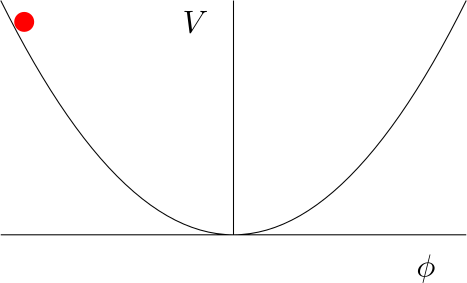
\includegraphics[scale=0.8]{vphi2}
  \caption{$V(\phi)=\frac{1}{2}\mu^2 \phi^2$ con $\mu^2\gt 0$} %noinstiki
  \label{fig:x2} %noinstiki
\end{figure} %noinstiki <div id="fig:x2">Figura: Un mínimo</div>
%noinstiki![cuerda](http://gfif.udea.edu.co/figfs/vphi2.png)
%noinstiki

Si $\mu^2\lt 0$, no existe un mínimo del potencial alrededor del cual el campo pueda oscilar. Además el alejamiento del campo del punto de simetría del potencial no cuesta energía. Por consiguiente en ese caso, el término de interacción
\begin{equation}
  V(\phi)=\tfrac{1}{2}\mu^2   \qquad 
  \mu^2\lt 0,
\end{equation}
no puede interpretarse como un término de masa en el Lagrangiano dado por la ec.~\eqref{eq:83qft}. 

Consideremos ahora el potencial
\begin{equation}
  V(\phi)=\tfrac{1}{2}\mu^2\phi^2+\tfrac{1}{4}\lambda\phi^4
  \qquad   \mu^2\lt 0,\ \lambda\gt 0
\end{equation}
que mantiene la simetría bajo la transformación discreta $\phi\to-\phi$. $\lambda\gt 0$ garantiza la aparición de los dos mínimos que se muestran el la figura \ref{fig:x2l}. Si la energía es suficientemente alta como se muestra en la figura~\ref{fig:x2l}, las excitaciones son simétricas con respecto al máximo del potencial y el término en $\mu^2$ no puede interpretarse como masa para la partícula escalar. 

%noinstiki
\begin{figure} %noinstiki
  \centering %noinstiki
  \includegraphics{vphi4}
  \caption{$V(\phi)=\frac{1}{2}\mu^2 \phi^2+\frac{1}{4}\lambda\phi^4$ con $\mu^2\lt 0$, y $\lambda\gt 0$. Simetría exácta} %noinstiki
  \label{fig:x2l} %noinstiki
\end{figure} %noinstiki <div id="fig:x2l">Figura: Mínimos degenerados</div>
%noinstiki![cuerda](http://gfif.udea.edu.co/figfs/vphi4.png)
%noinstiki
Sin embargo, si la energía es suficientemente baja como se muestra en la figura~\ref{fig:x2lm}, las excitaciones alrededor del mínimo dan lugar a la aparición de un término de masa para el campo escalar. Además, dichas excitaciones no respetan la simetrías $\phi\to-\phi$. En tal caso decimos que la simetría ha sido espontáneamente rota: aunque el Lagrangiano mantiene la simetría original, el vacío la rompe. 

%noinstiki
\begin{figure} %noinstiki
  \centering %noinstiki
  %noinstiki
  \includegraphics{vphi4m}
  \caption{$V(\phi)=\frac{1}{2}\mu^2 \phi^2+\frac{1}{4}\lambda\phi^4$ con $\mu^2\lt 0$, y $\lambda\gt 0$. Simetría espontáneamente rota.} %noinstiki
  \label{fig:x2lm} %noinstiki
\end{figure}  %noinstiki <div id="fig:x2lm">Figura: Simetría espontáneamente rota  </div>
%noinstiki![vphi4lm](http://gfif.udea.edu.co/figfs/vphi4lm.png)
%noinstiki

Para analizar cuantitativamente el espectro de partículas es necesario expandir el campo alrededor del mínimo y determinar las excitaciones. Establezcamos en primer lugar los mínimos del potencial. La $\partial V/\partial\phi=0$ da lugar a
\begin{align}
  \mu^2\phi+\lambda\phi^3&=0\\
  \phi(\mu^2+\lambda\phi^2)&=0,
\end{align}
con extremos $\phi_{\text{max}}=0$, y 
\begin{equation}
  \label{eq:90qft}
  \phi_{\text{min}}\equiv\langle\phi\rangle\equiv v=\pm\sqrt{\frac{-\mu^2}{\lambda}}.
\end{equation}
De hecho 
\begin{equation}
  \frac{\partial^2V}{\partial\phi^2}=\mu^2+3\lambda\phi^2.
\end{equation}
$\phi=0$ corresponde a un máximo, mientras que la segunda derivada para $\phi=\pm\sqrt{-\mu^2/\lambda}$ es $-2\mu^2\gt 0$ y corresponden a los mínimos. Expandiendo el campo alrededor del mínimo
\begin{equation}
  \phi(x)=H(x)+v
\end{equation}
\begin{align}
  V(\phi)=&\tfrac{1}{2}\mu^2 \phi^2+\tfrac{1}{4}\lambda\phi^4\nonumber\\
  =&\tfrac{1}{2}\mu^2 (H+v)^2+\tfrac{1}{4}\lambda(H+v)^4\nonumber\\
  =&\tfrac{1}{2}\mu^2 (H+v)^2+\tfrac{1}{4}\lambda(H+v)^4\nonumber\\
  =&\tfrac{1}{2}\mu^2 \left(H^2+2vH+v^2\right)+\tfrac{1}{4}\lambda\left(H^2+2vH+v^2\right)^2\nonumber\\
  =&\tfrac{1}{2}\mu^2 \left(H^2+2vH+v^2\right)+\tfrac{1}{4}\lambda\left[H^4+2H^2\left(2vH+v^2\right)+\left(2vH+v^2\right)^2\right]\nonumber\\
  =&\tfrac{1}{2}\mu^2 \left(H^2+2vH+v^2\right)+\tfrac{1}{4}\lambda\left[H^4+4vH^3+2H^2v^2+4v^2H^2+4v^3H+v^4\right]\nonumber\\
  =&\tfrac{1}{2}\mu^2 \left(H^2+2vH+v^2\right)+\tfrac{1}{4}\lambda\left[H^4+4vH^3+6H^2v^2+4v^3H+v^4\right]\nonumber\\
  =&\tfrac{1}{2}\mu^2H^2-\tfrac{3}{2}H^2\mu^2+\mu^2vH-\mu^2vH+\tfrac{1}{2}\mu^2v^2-\tfrac{1}{4}\mu^2v^2+\tfrac{1}{4}\lambda\left[H^4+4vH^3\right]\nonumber\\
\label{eq:84qft}
V(H)=&\tfrac{1}{2}\left(-2\mu^2\right)H^2+\lambda vH^3+\tfrac{1}{4}\lambda H^4+\tfrac{1}{4}\mu^2v^2,
\end{align}
y
\begin{equation}
  \label{eq:88qft}
  \mathcal{L}_H=\tfrac{1}{2}\partial^\mu H\partial_\mu H-\tfrac{1}{2}\left(-2\mu^2\right)H^2-\lambda vH^3-\tfrac{1}{4}\lambda H^4+\text{constant}.
\end{equation}
Entonces $H$ adquiere una masa $-2\mu^2$ y no es invariante bajo $H\to-H$. 

Otro método es usar las ecuaciones de mínimo $-\mu^2=\lambda v^2$, para eliminar un parámetro del potencial:
\begin{align}
  V(\phi)&=-\tfrac{1}{2}\lambda v^2\phi^2+\tfrac{1}{4}\lambda\phi^4\nonumber\\
  =&-\tfrac{1}{2}\lambda v^2 \left(H^2+2vH+v^2\right)+\tfrac{1}{4}\lambda\left[H^4+4vH^3+6H^2v^2+4v^3H+v^4\right]\nonumber\\
  =&\lambda v^2H^2+\lambda vH^3+\tfrac{1}{4}\lambda H^4+\text{constant}.
\end{align}
Podemos escribir el potencial en términos del  nuevo campo como
\begin{align}
\label{eq:higgspot}
  V(H)=\frac{1}{2}m_H^2H^2+\frac{1}{2}\frac{m_H^2}{v}H^3+\frac{1}{8}\frac{m_H^2}{v^2} H^4\,.
\end{align}
donde
\begin{equation}
\label{eq:higgsmass}
  m_H^2=2\left|\mu^2\right|=2\lambda v^2
\end{equation}

\subsection{Ausencia de taquiones}

Uno se podría preocupar por la presencia de un término de masa
imaginaria en el Lagrangiano, pero como estamos hablando de
transiciones de fase, estos porcesos deben suceder en presencia de
temperatura, por ejemplo la temperatura asociada al universo primitivo
durante las fases tempranas del Big Bang. En presencia de temperatura,
todas las partículas adquieren una masa térmica proporcional a la
temperatura como resultado de su interacción con el plasma. De este
modo, a altas temperaturas la masa de la partícula escalar esta
dominada por la temperatura y al ser positiva el potencial escalar
tiene un único mínimo simétrico. Cuando la temperatura baja lo
suficiente para que la masa al cuadrado negativa domine, el mínimo se
convierte en un máximo local altamente inestable y ocurre muy
rapidamente la transición de fase al nuevo mínimo no simétrico donde
la masa del escalar esta bien definida.

\subsection{Caso complejo}


Consideremos ahora un campo escalar complejo sin término de masa, pero con potencial:
\begin{equation}
  \label{eq:85qft}
  \mathcal{L}=\partial^\mu\phi^*\partial_\mu\phi-V(\phi)
\end{equation}
\begin{equation}
  V(\phi)=\mu^2\phi^*\phi+\lambda(\phi^*\phi)^2 
  \qquad 
  \mu^2\lt 0,\ \lambda\gt 0 
\end{equation}
La simetría del Lagrangiano corresponde a $U(1)$ global. Este potencial corresponde al ``sombrero mexicano'', como se ilustra en la Figura \ref{fig:mexicanhat}. Para una energía suficientemente baja de manera que el campo deba oscilar alrededor del mínimo aparecen dos tipos de excitaciones. Una sobre las paredes  que cuestan energía y corresponden a un campo escalar masivo como en el caso anterior, y otra a lo largo de la circunferencia de mínimo, que corresponde a una partícula escalar sin masa, y es llamada bosón del Golstone. 



\begin{figure}
  \centering
  \includegraphics[scale=0.5]{mexicanhat}
  \caption{Potential for complex scalar field}
  \label{fig:mexicanhat}
\end{figure}



El Lagrangiano escalar complejo es equivalente al Lagragiano de dos campos escalares reales con los mismos paramétros. Para un conjunto de $N$ campos reales tenedremos (suma sobre $i$) \cite{Peskin}\footnote{\S 11.1}: 
\begin{align}
  \mathcal{L}=\frac{1}{2}\partial^\mu\phi^i\partial_\mu\phi_i-\frac{1}{2}\mu^2\phi_i\phi^i-\frac{1}{2}\mu^2\left(\phi_i\phi^i\right)^2\,,
\end{align}
que es invariante bajo una simetría $O(N)$
\begin{align}
  \phi^i\to{\phi'}^i=R^{ij}\phi^j\,,
\end{align}
para cualquier matriz $N\times  N$ ortogonal $R$. El análisis para $N=2$ da lugar a un bosón de Goldstone. El anális para $N>2$ es el mismo y por cada campo real que se introduzca aparece un nuevo bosón de Goldstone \cite{Peskin}:
\begin{quote}
  [\ldots] there are not continuous symmetries for $N=1$, while for $N=2$ there is a single direction of rotation. A rotation in $N$ dimensions can be in any one of $N(N-1)$ planes, so the $O(N)$--symmetric theory has $N(N-1)/2$ continuous symmetries. After spontaneous symmetry breaking there are $(N-1)(N-2)/2$  remaining symmetries corresponding to rotations of the $(N-1)$ [non massive] fields. The number of \emph{broken} symmetries is the difference, $N-1$.
\end{quote}
Entonces tenemos el siguiente teorema \cite{Peskin}
\begin{quote}
\emph{Goldstone's theorem states that for every spontaneously broken continuous symmetry, the theory must contain a massless particle.}
\end{quote}

Also from \cite{Peskin}\footnote{Introduction to Chapter 20}
\begin{quote}
  In a global symmetry  that is spontaneously broken the symmetry currents are still conserved and interactions are similarly restricted [the Lagrangian keeps the symmetry], but the vacuum state does not respect the symmetry and the particles do not form obvious symmetry multiplets. Instead, such a theory contains massless particles, Goldstone bosons, one for each generator of the spontaneously broken symmetry. The third case is that of a local, or gauge, symmetry. [\ldots] such a symmetry requires the existence of a massless vector field for each symmetry generator, and the interactions among these fields are highly restricted.

It is now only natural to consider a fourth possibility: What happens if we include both local gauge invariance  and spontaneous symmetry breaking in the same theory?
\end{quote}
 
\section{Principio gauge local}



En el caso de la Acción invariante gauge local bajo el Grupo $U(1)$, tenemos el Lagrangiano 
\begin{equation}
  \label{eq:89qft}
  \mathcal{L}=\left(\mathcal{D}^\mu\phi\right)^*\mathcal{D}_\mu\phi-\mu^2\phi^*\phi-\lambda\left(\phi^*\phi\right)^2-\tfrac{1}{4}F^{\mu\nu}F_{\mu\nu}
  \qquad 
  \mu^2\lt 0\text{ and } \lambda\gt 0\,.
\end{equation}
Este es el Lagrangiano más general posible para un campo escalar complejo y el campo $A_\mu$ que deja la Acción invariante de Lorentz e invariante bajo la transformación gauge $U(1)$
\begin{align}
\label{eq:sqedgu}
  \phi(x)\to \phi'(x)=e^{i\theta(x)} \phi(x)\,,
\end{align}
En el caso de la superconductividad  electromagnético, $\phi$ representaría al campo escalar asociado al par de Cooper con carga eléctrica $-2$. Claramente el Lagrangiana en la ec.~\eqref{eq:89qft} es invariante local bajo tal $U(1)$ de carga eléctrica. 


\subsection{Gauge unitario}
Como $\phi$ es un campo complejo, podemos escribirlo en coordenadas polares con un campo real asociado a la magnitud del campo complejo y otro a la fase
\begin{align*}
  \phi(x)=\varphi(x)e^{i\eta(x)}
\end{align*}
Expandiendo el campo $\varphi(x)$ alrededor del mínimo: $\varphi(x)=(H(x)+v)/\sqrt{2}$, tenemos
\begin{align*}
    \phi(x)=e^{i\eta(x)}\left(\frac{H(x)+v}{\sqrt{2}}\right)\,.
\end{align*}


La libertad gauge nos permite en un momento determinado escoger la fase $\theta(x)$ de la ec.~\eqref{eq:sqedgu} sin que ese alteren los observables de la teoría. Para el campo en coordenadas polares tenemos que
\begin{align*}
     \phi\to\phi'=e^{i\theta(x)}e^{i\eta(x)}\left(\frac{H(x)+v}{\sqrt{2}}\right)
\end{align*}
Haciendo $\theta(x)=-\eta(x)$,
\begin{equation}
\label{eq:87qft}
   \phi\to\phi'=e^{-i\eta(x)+i\eta(x)}\left(\frac{H(x)+v}{\sqrt{2}}\right)=\frac{H(x)+v}{\sqrt{2}}
\end{equation}
\begin{align}
  \mathcal{L}\to\mathcal{L}' &=\left[\left(\mathcal{D}^\mu\right)'\phi'\right]^*\left(\mathcal{D}_\mu\right)'\phi'-\mu^2\left(\phi^*\right)'\phi'-\lambda\left[\left(\phi^*\right)'\phi'\right]^2-\tfrac{1}{4}\left(F^{\mu\nu}F_{\mu\nu}\right)'\nonumber\\
 &=\tfrac{1}{2}\left[\partial^\mu H+ig{A'}^\mu(H+v)\right]\left[\partial_\mu H-ig{A'}_\mu(H+v)\right]-\tfrac{1}{2}\mu^2(H+v)^2-\tfrac{1}{4}\lambda(H+v)^4-\tfrac{1}{4}\left(F^{\mu\nu}F_{\mu\nu}\right)'\,.
\end{align}
En adelante omitiremos las primas, aunque debe estar claro que se esta trabajando en el gauge específico de la ec.~\eqref{eq:87qft}. Entonces
\begin{align}
  \mathcal{L}&=\tfrac{1}{2}\partial^\mu H\partial_\mu H-\tfrac{1}{2}\mu^2(H+v)^2-
  \tfrac{1}{4}\lambda(H+v)^4+\tfrac{1}{2}g^2A^\mu A_\mu(H+v)^2
  -\tfrac{1}{4}F^{\mu\nu}F_{\mu\nu}.
\end{align}
Usando la ec.~\eqref{eq:84qft}
\begin{equation}
  \label{eq:94qft}
  \mathcal{L}=\mathcal{L}_H+\mathcal{L}_{A^\mu}+\tfrac{1}{2}g^2A^\mu A_\mu H^2+g^2vA^\mu A_\mu H,
\end{equation}
donde $\mathcal{L}_H$ esta dado por la ec.~\eqref{eq:88qft} y
\begin{equation}
  \mathcal{L}_{A^\mu}=-\tfrac{1}{4}F^{\mu\nu}F_{\mu\nu}+\tfrac{1}{2}g^2v^2A^\mu A_\mu.
\end{equation}
Teniendo en cuenta la ec.~\eqref{eq:23qft} para el Lagrangiano de Proca, vemos que como consecuencia de la ruptura espontánea de simetría el campo gauge ha adquirido una masa
\begin{equation}
  m_{A^\mu}=gv.
\end{equation}

El mecanismo completo mediante el cual, a partir de un Lagrangiano invariante gauge local, los bosones gauge adquieren masa se llama \emph{mecanismo de Higgs} \cite{Higgs:1964pj}. La partícula escalar que adquiere masa se llama Higgs, mientras que el bosón de Goldstone es absorbido por campo gauge como modo longitudinal. 

El número de grados de libertad independientes en el Lagrangiano original en la ec.~\eqref{eq:89qft} es cuatro. Correspondientes a los dos grados de libertad del bosón gauge no masivo y los dos del campo escalar complejo. En el Lagrangiano final en la ec.~\eqref{eq:94qft} no aparece el bosón de Goldstone. Sin embargo esto no es un problema porque dicho Lagrangiano también tiene cuatro grados de libertad correspondientes a  los tres grados de libertad del bosón gauge masivo y al grado de libertad del bosón de Higgs. 

\end{frame}

\subsection{Superconductivity}

El campo $H$ dentro del superconductor, que hereda la carga $-2$ de
$\phi$, rompe espontáneamente carga eléctrica para esa configuración
especial del vacío (mínimo de energía) donde se forma el condensado de
pares de Cooper. Pero el la acción claramente conserva en todo momento
la carga eléctrica.

A review ot the use of the Proca Equations for a massive photon in superconductivity is given in~\cite{massivephoton}. A popularization review along this lines is in the book of Frank Wilczek ``The Lightness of Being'' (see Additional references).

The photon mass inside a superconductor is $10^{-11}\,$GeV (or 1/1000 of the electron mass according to~\cite{massivephoton}). Also from the article in Beamline $\lambda\sim 10\ \mu\text{m}$ y $M_\gamma=\hbar/\lambda c$ %check numbers

There are two important length scales in a superconductor. The first measures how efficientrly the condensate expels a magnetic field. In fact, the expulsion is not 

Additional references:
\begin{itemize}
\item The Lightness of Being: Mass, Ether, and the Unification of Forces,
Frank Wilczek, \url{http://www.amazon.com/The-Lightness-Being-Unification-Forces/dp/0465018955}
\item \url{http://www.scholarpedia.org/article/Englert-Brout-Higgs-Guralnik-Hagen-Kibble_mechanism_(history)}
\item Elementary Particle Physics: Volume 1: Quantum Field Theory and ..., Volume 1
 By Yorikiyo Nagashima, \url{Elementary Particle Physics: Volume 1: Quantum Field Theory and ..., Volume 1
 By Yorikiyo Nagashima}
\item From Superconductors 
to Supercolliders
by LANCE DIXON \url{http://www.slac.stanford.edu/pubs/beamline/26/1/26-1-dixon.pdf}
\item Electrodynamics of Superconductors \url{http://www.physics.buffalo.edu/phy514/w11/index.html}
\end{itemize}


%\left(\right)
%%% Local Variables: 
%%% mode: latex
%%% TeX-master: "fullnotes"
%%% ispell-local-dictionary: "castellano8"
%%% End: 

%instiki:category: FisicaSubatomica

\chapter{Fermiones}
\label{cha:fermiones}
%instiki:
%instiki:***
%instiki:
%instiki:[[NotasFS|Tabla de Contenidos]]
%instiki:
%instiki:***
%instiki:
%instiki:* [Ecuaci\'on de Dirac](#ecuacion-de-dirac)
%instiki:
%instiki:* [Electrodin\'amica Cu\'antica](#electr-cuant)
%instiki:
%instiki:* [Cromodin\'amica Cu\'antica](#inter-fuert)
%instiki:
%instiki:* [Soluci\'on de part\'\i cula libre](#solucion-de-parti)
%instiki:
%instiki:***
%instiki:



\section{Fermiones quirales de cuatro componentes}
\label{sec:ferm-quir-de}

Sea
\begin{align}
  P_L\equiv&\frac{1-\gamma_5}{2}\nonumber\\
  P_R\equiv&\frac{1+\gamma_5}{2}\,.
\end{align}
Además
\begin{align}
  \psi_L\equiv P_L\psi\nonumber\\
  \psi_R\equiv P_R\psi\,.
\end{align}
Entonces
\begin{align}
  \psi=\psi_L+\psi_R\,.
\end{align}

Las matrices $P_{L,R}$ tienen las propiedades
\begin{align}
  P_L+P_R&=1 & P_{L,R}^2&=P_{L,R}P_{L,R}=P_{L,R}\nonumber\\
  P_L P_R&=0& P_{L,R}^\dagger&=P_{L,R}\,.
\end{align}
Usando la ec.~(\ref{eq:218qft})
\begin{align}
  P_{L,R}\gamma^\mu=\frac{1\mp\gamma_5}{2}\gamma^\mu=\gamma^\mu\frac{1\pm\gamma_5}{2}=\gamma^\mu P_{R,L}
\end{align}
Para escribir el Lagrangiano en término de los nuevos $\psi_{L,R}$ debemos tener en cuenta que
\begin{align}
  \overline{\psi_{L,R}}=(P_{L,R}\psi)^\dagger\gamma^0=\psi^\dagger P_{L,R}\gamma^0=\psi^\dagger\gamma^0P_{R,L}=\overline{\psi}P_{R,L}
\end{align}
\begin{align}
  \label{eq:221qft}
  \mathcal{L}=&i\overline{\psi}\gamma^\mu\partial_\mu\psi-m\overline{\psi}\psi\nonumber\\
  =&i\overline{\psi}(P_L+P_R)\gamma^\mu\partial_\mu\psi-m\overline{\psi}(P_L+P_R)\psi\nonumber\\
  =&i\overline{\psi}P_L\gamma^\mu\partial_\mu\psi+i\overline{\psi}P_R\gamma^\mu\partial_\mu\psi-m\overline{\psi}P_L\psi-m\overline{\psi}P_R\psi\nonumber\\
  =&i\overline{\psi}P_L P_L\gamma^\mu\partial_\mu\psi+i\overline{\psi}P_R P_R\gamma^\mu\partial_\mu\psi-m\overline{\psi}P_L P_L\psi-m\overline{\psi}P_R P_R\psi\nonumber\\
  =&i\overline{\psi}P_L\gamma^\mu\partial_\mu P_R\psi+i\overline{\psi}P_R\gamma^\mu\partial_\mu P_L\psi-m\overline{\psi}P_L P_L\psi-m\overline{\psi}P_R P_R\psi\nonumber\\
  =&i\overline{\psi_R}\gamma^\mu\partial_\mu\psi_R+i\overline{\psi_L}\gamma^\mu\partial_\mu\psi_L-m(\overline{\psi_R}\psi_L+\overline{\psi_L}\psi_R)\,.
\end{align}
En términos de espinores izquierdos y derechos de cuatro componentes la transformación de paridad 
\begin{align}
  \label{eq:220qft}
  t&\to t&\mathbf{x}&\to -\mathbf{x}&\psi_L(t,\mathbf{x})\to&\psi_R(t,-\mathbf{x}),& \psi_R(t,\mathbf{x})&\to\psi_L(t,-\mathbf{x})\nonumber\\
  \partial_0&\to \partial_0&\boldsymbol{\nabla}&\to -\boldsymbol{\nabla}&\psi_L(t,\mathbf{x})\to&\psi_R(t,-\mathbf{x}),& \psi_R(t,\mathbf{x})&\to\psi_L(t,-\mathbf{x})\,.
\end{align}
Además $\mathbf{L}=\mathbf{r}\times \mathbf{p}\to(-\mathbf{r})\times (-\mathbf{p})=\mathbf{L}$, y como $\gamma^\mu$ esta asociado al momento angular intrínsico, entonces también $\gamma^\mu\to\gamma^\mu$


Entonces la transformación de paridad da lugar a (sin tener en cuenta el cambio de argumento en los campos que desaparece en la integral de la Acción)
\begin{align}
  \overline{\psi_R}\gamma^\mu\partial_\mu\psi_R=\overline{\psi_R}\gamma^0\partial_0\psi_R+\overline{\psi_R}\boldsymbol{\gamma}\cdot\boldsymbol{\nabla}\psi_R 
\to&\overline{\psi_L}\gamma^0\partial_0\psi_L-\overline{\psi_L}\boldsymbol{\gamma}\cdot\boldsymbol{\nabla}\psi_L\nonumber\\
=&\overline{\psi_L}\gamma^0\partial_0\psi_L+\overline{\psi_L}\boldsymbol{\gamma}^\dagger\cdot\boldsymbol{\nabla}\psi_L\nonumber\\
=&\overline{\psi_L}\gamma^0\gamma^0\gamma^0\partial_0\psi_L+\overline{\psi_L}\gamma^0\boldsymbol{\gamma}\gamma^0\cdot\boldsymbol{\nabla}\psi_L\nonumber\\
=&\overline{\psi_L}\tilde\gamma^0\partial_0\psi_L+\overline{\psi_L}\tilde{\boldsymbol{\gamma}}\cdot\boldsymbol{\nabla}\psi_L\nonumber\\
=&\overline{\psi_L}\tilde\gamma^\mu\partial_\mu\psi_L\,.
\end{align}
Entonces
\begin{align}
   \mathcal{L}\to\mathcal{L}'=&i\overline{\psi_R}\tilde\gamma^\mu\partial_\mu\psi_R+i\overline{\psi_L}\tilde\gamma^\mu\partial_\mu\psi_L-m(\overline{\psi_R}\psi_L+\overline{\psi_L}\psi_R)\,,
\end{align}
donde $\tilde\gamma^\mu=U\gamma^\mu U^\dagger$, con $U=\gamma^0$. Como las dos representaciones dan lugar a la misma física, podemos decir que la Acción en términos de espinores $L,R$ de cuatro componentes es invariante bajo la transformación de paridad.

La existencia de ambos espinores $\psi_{L,R}$ garantizan que el Lagrangiano de Dirac es invariante bajo la transformación de paridad. 

La corriente de la electrodinámica cuántica en ec.~\eqref{eq:222qft} (o la de la cromodinámica cuántica, ec.~\eqref{eq:223qft}) conservan paridad ya que, siguiendo los mismos pasos que en la ec.~\eqref{eq:221qft}
\begin{align}
  \label{eq:224qft}
  \overline{\psi}\gamma^\mu\psi=\overline{\psi_L}\gamma^\mu\psi_L+\overline{\psi_R}\gamma^\mu\psi_R\to\overline{\psi_L}\tilde{\gamma}^\mu\psi_L+\overline{\psi_R}\tilde{\gamma}^\mu\psi_R\,.
\end{align}
Si para alguna partícula, como es el caso del neutrino, no existe la componente derecha, entonces la correspondiente interacción vectorial viola paridad y no puede tener ni interacciones electromagnéticas ni fuertes, es decir, no se acopla con el fotón o los gluones. Además dicha partícula no puede tener masa de Dirac. En el caso del neutrino esto se entiende pues al no tener carga eléctrica sólo requiere dos grados de libertad independientes.

De otro lado, si una determinada interacción, como es el caso de la interacción débil, solo participa la componente izquierda de la ec.~\eqref{eq:224qft}, está corresponde a una interacción del tipo
\begin{align}
  \overline{\psi}_L\gamma^\mu\psi_L&=\overline{\psi}P_R\gamma^\mu P_L\psi=\overline{\psi}\gamma^\mu P_L\psi\nonumber\\
  &=\overline{\psi}\gamma^\mu\left(\frac{1-\gamma_5}{2}\right)\psi\nonumber\\
  &=\tfrac{1}{2}\overline{\psi}\left(\gamma^\mu-\gamma^\mu\gamma_5\right)\psi\,,
\end{align}
que de acuerdo a la asignación en la Tabla corresponde a una corriente V--A. 

\subsection{Fermiones de Weyl}
\label{sec:fermiones-de-weyl}
%Weyl because $\psi^\dagger$ instead $\bar \psi$
Sea $\psi$ un campo que satisface una ecuaci\'on covariante de segundo orden. La parte cin\'etica del Lagrangiano sin t\'erminos de masa y sin t\'erminos de interacci\'on debe tener la forma 
\begin{equation}
\label{eq:98}
  \mathcal{L}=\frac{i}{2}\psi^\dagger a^\mu\partial_\mu\psi-\frac{i}{2}\partial_\mu\psi^\dagger {a^\mu}^\dagger\psi-m\psi^\dagger b\psi
\end{equation}
La Acci\'on debe ser real, de modo que el Lagrangiano tambi\'en. En efecto
\begin{align*}
  \mathcal{L}^\dagger&=\left(\frac{i}{2}\psi^\dagger a^\mu\partial_\mu\psi-\frac{i}{2}\partial_\mu\psi^\dagger {a^\mu}^\dagger\psi\right)^\dagger-m\psi^\dagger b^\dagger \psi\\
  &=\left(-\frac{i}{2}\partial^\mu\psi^\dagger a_\mu^\dagger \psi+\frac{i}{2}\psi^\dagger {a^\mu} \partial_\mu\psi\right)-m\psi^\dagger b^\dagger \psi\\
  &=\mathcal{L} \qquad \text{si }b^\dagger = b\,.
\end{align*}
Como al aplicar las ecuaciones de Euler-Lagrange a este Lagrangiano debemos obtener la ecuaci\'on de Scrh\"odinger
\begin{align}
i\frac{\partial}{\partial t}\psi=\widehat{H}\psi
\end{align}
con $\widehat{H}$ una funci\'on por determinar del operador $\hat{\mathbf{p}}$, entonces
\begin{align}
  a_\mu^\dagger=a_\mu
\end{align}

El Lagrangiano en ec.~(\ref{eq:98}) puede reescribirse como
\begin{align}
  \label{eq:197}
  \mathcal{L}&=\frac{i}{2}\psi^\dagger a^\mu\partial_\mu\psi-\frac{i}{2}\partial_\mu\left(\psi^\dagger a^\mu\psi\right)+\frac{i}{2}\psi^\dagger a^\mu\partial_\mu\psi-m\psi^\dagger b\psi\nonumber\\
  &=i \psi^\dagger a^\mu\partial_\mu\psi-\frac{i}{2}\partial_\mu\left(\psi^\dagger a^\mu\psi\right)-m\psi^\dagger b\psi\nonumber\\
  \mathcal{L}&=i \psi^\dagger a^\mu\partial_\mu\psi-m\psi^\dagger b\psi
\end{align}

Ahora utilizaremos el m\'etodo desarrollado en cap\'\i tulos anteriores para analizar el Lagrangiano. Calcularemos las ecuaciones de Euler-Lagrange, la corriente conservada y el tensor de momento-energ\'\i a.


\section{Soluciones a la ecuaci\'on de Dirac}
\label{sec:soluc-la-ecuac}

\subsection{Lagrangiano de Weyl}
\label{sec:lagrangiano-de-weyl}


En la ec.~\eqref{eq:118}, obtuvimos el Hamiltoniano en ec.~\eqref{eq:103}
\begin{equation}
  \hat{H}= \gamma_0(\boldsymbol{\gamma}\cdot\mathbf{p}+m)=\boldsymbol{\alpha}\cdot\mathbf{p}+\beta m\,.
\end{equation}
Una escogencia particular de las cuatro matrices $\gamma^\mu$, conocida como la representaci\'on de Weyl, o representaci\'on quiral, puede escribirse en t\'erminos de la matrices de Pauli. Escritas en bloques $2\times2$, tenemos
\begin{equation}
  \gamma^0=
  \begin{pmatrix}
    0&\sigma_0\\
    \sigma_0&0
  \end{pmatrix}\qquad
  \gamma_i=\begin{pmatrix}
    0&\sigma_i\\
    -\sigma_i&0
  \end{pmatrix}.
\end{equation}
Con $\sigma^0=1$. Con la matriz de tranformaci\'on
\begin{equation}
  U=\frac{1}{\sqrt{2}}
  \begin{pmatrix}
    1&1\\
    -1&1    
  \end{pmatrix}
\end{equation}
podemos obtener la representaci\'on de Dirac, tal que $U$ diagonaliza $\gamma^0$,
\begin{equation}
  \gamma^0=
  \begin{pmatrix}
    \sigma^0&0\\
    0&-\sigma^0
  \end{pmatrix}\qquad
  \gamma_i=\begin{pmatrix}
    0&\sigma_i\\
    -\sigma_i&0
  \end{pmatrix}.
\end{equation}
En adelante trabajaremos en la representaci\'on de Weyl que en forma compacta es
\begin{equation}
  \gamma^\mu=\begin{pmatrix}
    0&\sigma^\mu\\
    \bar{\sigma}^\mu & 0
  \end{pmatrix}
\end{equation}
donde
\begin{align}
  \sigma^\mu&=(\sigma^0,\sigma^1,\sigma^2,\sigma^3)\nonumber\\
  \bar{\sigma}^\mu&=(\sigma^0,-\sigma^1,-\sigma^2,-\sigma^3)\nonumber\\
\end{align}
Hemos escrito las matrices de Dirac en bloques $2\times2$, y es natural escribir similarmente las cuatro componentes del campo de Dirac como un par de campos de dos componentes
\begin{align}
  \psi=  \begin{pmatrix}
    \psi_L\\
    \psi_R    
  \end{pmatrix}=\begin{pmatrix}
    \psi_L\\
    0   
  \end{pmatrix}+\begin{pmatrix}
    0\\
    \psi_R    
  \end{pmatrix}
\end{align}
Donde $\psi_{L,R}$ son espinores de Weyl de dos componentes. En la representaci\'on de Weyl el Lagrangiano se puede escribir como
\begin{align}
\label{eq:200}
  \mathcal{L}=&i\bar{\psi}\gamma^\mu\partial_\mu\psi-m\bar{\psi}\psi\nonumber\\
  =&i\psi^\dagger \gamma^0\gamma^\mu\partial_\mu\psi-m\psi^\dagger \gamma^0 \psi\nonumber\\
  =&i\psi^\dagger  \begin{pmatrix}
    0 & 1\\
    1&0
  \end{pmatrix}
  \begin{pmatrix}
    0 &\sigma^\mu \\
    \bar{\sigma}^\mu&0
  \end{pmatrix}\partial_\mu\psi-m\psi^\dagger
  \begin{pmatrix}
    0 & 1\\
    1&0
  \end{pmatrix}\psi\nonumber\\
=&i\begin{pmatrix}
 \psi_L^\dagger & \psi_R^\dagger
\end{pmatrix}
 \begin{pmatrix}
   \bar{\sigma}^\mu &0\\
   0&\sigma^\mu
 \end{pmatrix} \begin{pmatrix}
   \partial_\mu\psi_L\\
   \partial_\mu\psi_R
 \end{pmatrix}-m
 \begin{pmatrix}
   \psi_L^\dagger&\psi_R^\dagger
 \end{pmatrix}
 \begin{pmatrix}
   0&1\\
   1&0
 \end{pmatrix}
 \begin{pmatrix}
   \psi_L\\ \psi_R
 \end{pmatrix}\nonumber\\
 =& i\psi_L^\dagger \bar{\sigma}^\mu\partial_\mu\psi_L+i\psi_R^\dagger \sigma^\mu\partial_\mu\psi_R
  -m(\psi_L^\dagger \psi_R+\psi_R^\dagger \psi_L)
\end{align}

\subsection{Ecuaciones de Weyl}
\label{sec:ecuaciones-de-weyl}
Las ecuaciones de Euler-Lagrango para el Lagrangiano en ec.\eqref{eq:200}, dan como resultado
\begin{align}
  i\bar{\sigma}^\mu\partial_\mu\psi_L -m\psi_R &=0\nonumber\\
  i{\sigma}^\mu\partial_\mu\psi_R -m\psi_L &=0
\end{align}
Expandiendo
\begin{align}
  \label{eq:209}
   i{\sigma}^0\partial_0\psi_L-i{\sigma}^i\partial_i\psi_L -m\psi_R &=0\nonumber\\
   i{\sigma}^0\partial_0\psi_R+i{\sigma}^i\partial_i\psi_R -m\psi_L &=0
\end{align}
que pueden escribirse como
\begin{align}
  \label{eq:207}
   i\partial_0\psi_L-i\boldsymbol{\sigma}\cdot\boldsymbol{\nabla}\psi_L -m\psi_R &=0\nonumber\\
   i\partial_0\psi_R+i\boldsymbol{\sigma}\cdot\boldsymbol{\nabla}\psi_R -m\psi_L &=0
\end{align}
Para el Lagrangiano invariante gauge local $U(1)$ en ec.\eqref{eq:201}, tendr\'\i amos
\begin{align}
  i\bar{\sigma}^\mu\mathcal{D}_\mu\psi_L -m\psi_R &=0\nonumber\\
  i{\sigma}^\mu\mathcal{D}_\mu\psi_R -m\psi_L &=0
\end{align}
Expandiendo, para $\mathcal{D}^\mu$ dado en la ec.\eqref{eq:202}, con $q=-e$
\begin{equation}
  \mathcal{D}_\mu=\partial_\mu+i q A_\mu
\end{equation}
Tenemos
\begin{align}
     i(\partial_0+i q A_0)\psi_L-i{\sigma}^i(\partial_i+i q A_i)\psi_L -m\psi_R &=0\nonumber\\
   i(\partial_0+i q A_0)\psi_R+i{\sigma}^i(\partial_i+i q A_i)\psi_R -m\psi_L &=0
\end{align}
de donde
\begin{align}
\label{eq:203}
     (i\partial_0- q A_0)\psi_L-{\sigma}^i(i\partial_i-q A_i)\psi_L -m\psi_R &=0\nonumber\\
   (i\partial_0-q A_0)\psi_R+{\sigma}^i(i\partial_i-q A_i)\psi_R -m\psi_L &=0
\end{align}
\section{Esp\'\i n}
\label{sec:espin}
El momento angular est\'a descrito por el \'algebra
\begin{equation}
  [\hat L_i,\hat L_j]=i\epsilon_{ijk}\hat L_k
\end{equation}
Si dos operadores no conmutan no es posible conocer sus autovalores simult\'aneamente. Sin embargo
\begin{equation}
  [\hat L_i,\hat{L}^2]=0
\end{equation}
y por convenci\'on podemos escoger $\langle\hat L_z\rangle$ y $\hat{L}^2$ como los dos observables de momento \'angular. 

Las matrices de Pauli forman una representaci\'on del \'algebra de momento angular
\begin{equation}
  [\hat S_i,\hat S_j]=i\epsilon_{ijk}\hat S_k
\end{equation}
donde el \emph{operador de esp\'\i n} se define como
\begin{equation}
  \hat S_i=\frac{\sigma_i}{2}
\end{equation}
Los autovalores del operador de esp\'\i n son entonces
\begin{equation}
  \hat S_z
  \begin{pmatrix}
    a\\
    b
  \end{pmatrix}=\lambda
  \begin{pmatrix}
    a\\
    b
  \end{pmatrix}
\end{equation}
que corresponde a autovalores $\lambda=\pm1/2$ con autovectores 
\begin{equation}
  |\uparrow\rangle=\begin{pmatrix}
    1\\
    0
  \end{pmatrix}\qquad
  |\downarrow\rangle=\begin{pmatrix}
    0\\
    1
  \end{pmatrix}
\end{equation}
que son autoestados de esp\'\i n up y esp\'\i n down respectivamente. Una funci\'on de onda de esp\'\i n ha de poder expandir en t\'erminos de estos autoestados
\begin{equation}
  |\psi\rangle=c_1|\uparrow\rangle+c_2|\downarrow\rangle
\end{equation}
donde $|c_1|^2$ y $|c_2|^2$ corresponden a las probabilidades de encontrar el estado con esp\'\i n up o esp\'\i n down respectivamente. Adem\'as
\begin{equation}
  |c_1|^2+|c_2|^2=1
\end{equation}
y $\psi$ es un espinor. La ecuaci\'on de Scr\"odinger para un espinor es, por ejemplo
\begin{align}
  i\frac{\partial\psi_R}{\partial t}=\widehat{H}\psi_R
\end{align}
donde
\begin{equation}
  \psi_R=
  \begin{pmatrix}
    \psi_1\\
    \psi_2
  \end{pmatrix}
\end{equation}
con $\psi_i$ las funciones de onda convencionales. Dicha ecuaci\'on debe ser invariante bajo rotaciones en el espacio de esp\'\i n
\begin{equation}
  \psi_R\to\psi'_R=\exp(i\frac{\sigma^i}{2}\theta_i)\psi_R\,.
\end{equation}
Esta es justo las ecuaciones que aparecen cuando se hace $m=0$ en la ec.\eqref{eq:207}. Para $\psi_R$
\begin{equation}
  \widehat{H}=i\boldsymbol{\sigma}\cdot\boldsymbol{\nabla}=-\boldsymbol{\sigma}\cdot\mathbf{p}
\end{equation}
con
\begin{align}
\label{eq:208}
\mathcal{L}&= i\psi_R^\dagger {\sigma}^\mu\partial_\mu\psi_R  \nonumber\\
&=i\psi_R^\dagger \partial_0\psi_R+i\psi_R^\dagger {\sigma}^i\partial_i\psi_R\nonumber\\
&=i\psi_R^\dagger \partial_0\psi_R-i\psi_R^\dagger\boldsymbol{\sigma}\cdot\mathbf{p} \psi_R
\end{align}
Como el Lagrangiano debe ser escalar entonces $\psi_R^\dagger\boldsymbol{\sigma} \psi_R$ debe ser un vector en el espacio de esp\'\i n. En efecto, escogiendo los coeficientes como
\begin{align}
  c_1&=e^{-i \phi/2}\cos(\theta/2)\nonumber\\
  c_2&=e^{i \phi/2}\sin(\theta/2)
\end{align}
entonces
\begin{equation}
  |c_1|^2+|c_2|^2=c_1 c_1^*+c_2 c_2^*=\cos^2(\theta/2)+\sin^2(\theta/2)=1\,.
\end{equation}
Para
\begin{align}
  \psi_R=e^{-i p\cdot x}(c_1|\uparrow\rangle+c_2|\downarrow\rangle)&=e^{-i p\cdot x}\left[c_1\begin{pmatrix}
    1\\
    0
  \end{pmatrix}+c_2
  \begin{pmatrix}
    0\\
    1
  \end{pmatrix}\right]=
  e^{-i p\cdot x}\begin{pmatrix}
    c_1\\
    c_2
  \end{pmatrix}\,\nonumber\\
  &=e^{-i p\cdot x}
  \begin{pmatrix}
  e^{-i \phi/2}\cos(\theta/2)\\
  e^{i \phi/2}\sin(\theta/2)
  \end{pmatrix}=e^{-i p\cdot x}|+\rangle
\end{align}
donde
\begin{equation}
|+\rangle=  \begin{pmatrix}
  e^{-i \phi/2}\cos(\theta/2)\\
  e^{i \phi/2}\sin(\theta/2)
  \end{pmatrix}\,.
\end{equation}
Tenemos
\begin{align}
  \psi^\dagger_R \sigma_1 \psi_R=&
  \begin{pmatrix}
   c_1^\dagger & c_2^\dagger 
  \end{pmatrix}
  \begin{pmatrix}
    0 & 1\\
    1&0
  \end{pmatrix}
  \begin{pmatrix}
    c_1\\
    c_2
  \end{pmatrix}\nonumber\\
  =&  \begin{pmatrix}
    c_2^\dagger & c_1^\dagger
  \end{pmatrix}
  \begin{pmatrix}
    c_1\\
    c_2
  \end{pmatrix}\nonumber\\
  =&  c_2^\dagger c_1 + c_1^\dagger c_2\nonumber\\
  =&  \sin(\theta/2)\cos(\theta/2)e^{-i\phi}+\cos(\theta/2)\sin(\theta/2)e^{i\phi}\nonumber\\
  =&  (e^{-i\phi}+e^{i\phi})\cos(\theta/2)\sin(\theta/2)\nonumber\\
  =&  (2\cos\phi)\frac{1}{2}\sin\theta\nonumber\\
  =&  \cos\phi\sin\theta
\end{align}
Similarmente
\begin{align}
  \psi^\dagger_R \sigma_2\psi_R&=\sin\phi\sin\theta\nonumber\\
  \psi^\dagger_R \sigma_3\psi_R&=\cos\theta
\end{align}
Por consiguiente $\psi^\dagger \sigma_i\psi$ son las componentes de un vector unitario $\psi^\dagger \boldsymbol{\sigma}\psi$ con \'angulo polar $\theta$ y \'angulo azimutal $\phi$. Posibles escalares se pueden construir con otros vectores disponibles, por ejemplo $\mathbf{p}$, como en la ec.~\eqref{eq:208}.
\begin{align}
  \boldsymbol{\sigma}\cdot\hat{\mathbf{p}}=&\sigma^i \frac{p^i}{|\mathbf{p}|}\nonumber\\
  =&\sigma^1\cos\phi\sin\theta+\sigma^2\sin\phi\sin\theta+\sigma^3\cos\theta\nonumber\\
  =&\begin{pmatrix}
    \cos\theta&\sin\theta(\cos\phi-i\sin\phi)\\
    \sin\theta(\cos\phi-i\sin\phi)&-\cos\theta
  \end{pmatrix}\nonumber\\
  =&\begin{pmatrix}
    \cos\theta&e^{-i\phi}\sin\theta\\
    e^{i\phi}\sin\theta&-\cos\theta
  \end{pmatrix}
\end{align}
\begin{align}
\boldsymbol{\sigma}\cdot\hat{\mathbf{p}}|+\rangle=&\begin{pmatrix}
    \cos\theta&e^{-i\phi}\sin\theta\\
    e^{i\phi}\sin\theta&-\cos\theta
  \end{pmatrix}\begin{pmatrix}
  e^{-i \phi/2}\cos(\theta/2)\\
  e^{i \phi/2}\sin(\theta/2)
  \end{pmatrix}\nonumber\\
  =&e^{-i\phi/2}\begin{pmatrix}
    \cos\theta&e^{-i\phi}\sin\theta\\
    e^{i\phi}\sin\theta&-\cos\theta
  \end{pmatrix}\begin{pmatrix}
  \cos(\theta/2)\\
  e^{i \phi}\sin(\theta/2)
  \end{pmatrix}\nonumber\\
  =&e^{-i\phi/2}
  \begin{pmatrix}
    \cos\theta\cos(\theta/2)+\sin\theta\sin(\theta/2)\\
    e^{i\phi}[\sin\theta\cos(\theta/2)- \cos\theta\sin(\theta/2)]
  \end{pmatrix}\nonumber\\
  =&e^{-i\phi/2}
  \begin{pmatrix}
    \cos(\theta-\theta/2)\\
    e^{i\phi}\sin(\theta-\theta/2)
  \end{pmatrix}\nonumber\\
  =&e^{-i\phi/2}
  \begin{pmatrix}
    \cos(\theta/2)\\
    e^{i\phi}\sin(\theta/2)
  \end{pmatrix}\nonumber\\
  =&+|+\rangle
\end{align}
(El gorro en este caso, significa vector unitario). Decimos entonces que
\begin{align}
\label{eq:214}
\boldsymbol{\sigma}\cdot\hat{\mathbf{p}}\psi_R=+e^{-i p\cdot x}|+\rangle=+\psi_R
\end{align}
es un estado de helicidad positiva o derecha. Como $\boldsymbol{\sigma}\cdot\mathbf{p}$ denota la proyecci\'on de esp\'\i n sobre la direcci\'on de moviento, para la helicidad derecha, dicha proyecci\'on es positiva.


Si definimos ademas
\begin{equation}
  \psi_L=e^{-i p\cdot x}|-\rangle
\end{equation}
donde
\begin{equation}
|-\rangle=  \begin{pmatrix}
  -e^{-i \phi/2}\sin(\theta/2)\\ 
  e^{i \phi/2}\cos(\theta/2)
  \end{pmatrix}\,,
\end{equation}
entonces
\begin{align}
  \psi^\dagger\boldsymbol{\sigma}\cdot\hat{\mathbf{p}}\psi=-(\cos\phi\sin\theta,\sin\phi\sin\phi,\cos\theta)
\end{align}
y
\begin{equation}
  \label{eq:215}
  \boldsymbol{\sigma}\cdot\hat{\mathbf{p}}\psi_L=-e^{-i p\cdot x}|-\rangle=-\psi_L
\end{equation}
$\psi$ es un estado de helicidad negativa o izquierda. Adem\'as
\begin{align}
  \langle-|-\rangle=\langle+|+\rangle=1\qquad \langle+|-\rangle=\langle-|+\rangle=0
\end{align}
donde $\langle-|=|-\rangle^\dagger$, etc.
%\left(\right)
\section{Soluci\'on de part\'\i cula libre}
\label{sec:solucion-de-parti}
Consideraremos incialmente dos casos $m^2\gg\mathbf{p}^2$ y $m^2\ll\mathbf{p}^2$.

De la ecuaci\'on relativista
\begin{equation}
  \label{eq:213}
  E^2=\mathbf{p}^2+m^2\,,
\end{equation}
tenemos que para elcaso no relativista $m^2\gg\mathbf{p}^2$, podemos tomar $\mathbf{p}=0$, de modo que
\begin{equation}
  E^2=m^2\Rightarrow E=\pm m
\end{equation}
La aparici\'on de soluciones de Energ\'\i a negativa. . .

A $\mathbf{p}=0$ proponemos las soluciones de energ\'\i a positiva $E=+m$
\begin{align}
  \label{eq:210}
  \psi_L&=u_L e^{-i E t}=\psi_L=u_L e^{-i m t} & \psi_R&=u_R e^{-i E t}=u_R e^{-i m t}
\end{align}

En este caso las ecs.~\eqref{eq:207} se reducen a
\begin{align}
  i\partial_0\psi_L -m\psi_R &=0\nonumber\\
  i\partial_0\psi_R -m\psi_L &=0
\end{align}
de modo que para que \eqref{eq:210} sea soluci\'on, se debe satisfacer que 
\begin{equation}
  u_L=u_R=u
\end{equation}
con
\begin{align}
  u=  \begin{pmatrix}
    u_1\\
    u_2    
  \end{pmatrix}=|+\rangle\,.
\end{align}
El espinor completo es
\begin{align}
  \psi=\begin{pmatrix}
    \psi_L\\
    \psi_R
  \end{pmatrix}=e^{-i m t}\begin{pmatrix}
    |+\rangle\\
    |+\rangle
  \end{pmatrix}
\end{align}
Con norma
\begin{align}
  \bar{\psi}\psi=\psi^\dagger\gamma^0\gamma^0\psi=\psi^\dagger\psi=|+\rangle^\dagger|+\rangle+|+\rangle^\dagger|+\rangle=1
\end{align}
Para el caso relativista $m^2\ll\mathbf{p}^2$, podemos hacer $m=0$ y las ecuaciones \eqref{eq:207} se desacoplan
\begin{align}
  \label{eq:211}
   i\partial_0\psi_L-i\boldsymbol{\sigma}\cdot\boldsymbol{\nabla}\psi_L &=0\nonumber\\
   i\partial_0\psi_R+i\boldsymbol{\sigma}\cdot\boldsymbol{\nabla}\psi_R&=0
\end{align}
Proponemos como soluciones de energ\'\i a positiva
\begin{align}
  \label{eq:212}
    \psi_L&=u_L e^{-i p\cdot x}=\psi_L=u_L e^{i(\mathbf{p}\cdot \mathbf{x}-E t)} & \psi_R&=u_R e^{-i p\cdot x}=u_R e^{i(\mathbf{p}\cdot \mathbf{x}-E t)}
\end{align}
reemplazando en las ecs.~\eqref{eq:211} tenemos
\begin{align}
  \label{eq:217}
     E\psi_L+\boldsymbol{\sigma}\cdot\mathbf{p}\psi_L &=0\nonumber\\
   E\psi_R-\boldsymbol{\sigma}\cdot\mathbf{p}\psi_R&=0
\end{align}
De modo que para que las ecs.~\eqref{eq:212} sean soluci\'on se debe satisfacer que
\begin{align}
     \boldsymbol{\sigma}\cdot\frac{\mathbf{p}}{E}\psi_L &=-\psi_L\nonumber\\
   \boldsymbol{\sigma}\cdot\frac{\mathbf{p}}{E}\psi_R&=\psi_R
\end{align}
pero de la ec.~\eqref{eq:213}, tenemos que para $m=0$, $E=|\mathbf{p}|$, y $\mathbf{p}/E=\mathbf{p}/|\mathbf{p}|=\hat{\mathbf{p}}$. Entonces
\begin{align}
  \boldsymbol{\sigma}\cdot\hat{\mathbf{p}}\psi_L &=-\psi_L\nonumber\\
  \boldsymbol{\sigma}\cdot\hat{\mathbf{p}}\psi_R&=\psi_R
\end{align}
Comparando con las ecuaciones \eqref{eq:214} y \eqref{eq:215} vemos que para las soluciones de energ\'\i a positiva $\psi_{R,L}$ corresponden en efecto a estado de helicidad derecha e izquierda respectivamente. Explicitamente
\begin{equation}
  \boldsymbol{\sigma}\cdot\hat{\mathbf{p}}\psi_L=e^{-i p\cdot x}\boldsymbol{\sigma}\cdot\hat{\mathbf{p}}|-\rangle=-e^{-i p\cdot x}|-\rangle=-\psi_L
\end{equation}
El espinor de cuatro componentes para la soluci\'on de energ\'\i a positiva es
\begin{equation}
  \psi=\begin{pmatrix}
    \psi_L\\
    \psi_R
  \end{pmatrix}=e^{-i p\cdot x}\begin{pmatrix}
    |-\rangle\\
    |+\rangle
  \end{pmatrix}
\end{equation}

\begin{align}
  \bar{\psi}\psi=&\bar{u}{u}=\psi^\dagger \gamma^0 \psi\nonumber\\
  =&\begin{pmatrix}
    |-\rangle^\dagger & |+\rangle^\dagger
  \end{pmatrix}
  \begin{pmatrix}
    0&1\\
    1&0    
  \end{pmatrix}
  \begin{pmatrix}
    |-\rangle\\
    |+\rangle
  \end{pmatrix}\nonumber\\
  =&\begin{pmatrix}
    \langle-| & \langle+|
  \end{pmatrix}
  \begin{pmatrix}
    0&1\\
    1&0    
  \end{pmatrix}
  \begin{pmatrix}
    |-\rangle\\
    |+\rangle
  \end{pmatrix}\nonumber\\
  =&\begin{pmatrix}
    \langle+| & \langle-| 
  \end{pmatrix}
  \begin{pmatrix}
    |-\rangle\\
    |+\rangle
  \end{pmatrix}\nonumber\\
  =&\langle+|-\rangle+\langle-|+\rangle=0
\end{align}

Es convenci\'on escoger la normalizaci\'on del espinor de Dirac tal que
\begin{equation}
  \bar{u}{u}=2m
\end{equation}
que de hecho es cero cuando $m=0$.

Para las soluciones de energ\'\i a negativa tenemos

\begin{align}
    \hat{\psi}_L&=u_L e^{i(\mathbf{p}\cdot \mathbf{x}+E t)} & \hat{\psi}_R&=u_R e^{i(\mathbf{p}\cdot \mathbf{x}+E t)}
\end{align}
Para explorar las caracter\'\i sticas de esta soluci\'on podemos reemplazar en la ec.~(\ref{eq:217}) $E\to-E$, $\mathbf{p}\to\mathbf{p}$, de modo que
\begin{align}
  \boldsymbol{\sigma}\cdot\hat{\mathbf{p}}\hat{\psi}_L &=+\hat{\psi}_L\nonumber\\
  \boldsymbol{\sigma}\cdot\hat{\mathbf{p}}\hat{\psi}_R&=-\hat{\psi}_R
\end{align}
De modo que la antipart\'\i cula de una part\'\i cula de helicidad izquierda tiene helicidad derecha. Dentro de los errores experimentales actuales se puede afirmar que en la naturaleza solo se ha observado el neutrino izquierdo y su correspondiente antineutrino derecho.

Para $m\neq0$, tenemos de la ecs.~\eqref{eq:207} y \eqref{eq:212} (ver ec.~\eqref{eq:217})
\begin{align}
  E\psi_L+\boldsymbol{\sigma}\cdot\mathbf{p}\psi_L &=m\psi_R\nonumber\\
  E\psi_R-\boldsymbol{\sigma}\cdot\mathbf{p}\psi_R&=m\psi_L
\end{align}
Entonces
\begin{align}
  \label{eq:219}
  \left(\frac{E+\boldsymbol{\sigma}\cdot\mathbf{p}}{m}\right)\psi_L&=\psi_R\nonumber\\
  \left(\frac{E-\boldsymbol{\sigma}\cdot\mathbf{p}}{m}\right)\psi_R&=\psi_L\,.
\end{align}
En este caso sin embargo, la helicidad no esta bien definida y s\'olo podemos afirmar que $\psi_L$ corresponde a la soluci\'on que tiene mayor probabilidad de ser izquierda que derecha. Para calcular dicha probabilidad es necesario especificar los espinores $u_{L,R}$ (ver \cite{cottingham}, Cap\'\i tulo 6). El resultado es que la probabilidad de que $\psi_{R}$ sea derecho se obtiene de
\begin{align}
  \boldsymbol{\sigma}\cdot\mathbf{p}|\psi_{R}\rangle&=+\frac{1}{2}\left(1+\frac{v}{c}\right)|\psi_{R}\rangle\to 
  \begin{cases}
    +|\psi_{R}\rangle & v\to c\quad\text{(relativistic)}\\
    +\frac{1}{2}|\psi_{R}\rangle & v\to 0 \quad\text{(non-relativistic)}
  \end{cases}\nonumber\\
  \boldsymbol{\sigma}\cdot\mathbf{p}|\psi_{L}\rangle&=-\frac{1}{2}\left(1-\frac{v}{c}\right)|\psi_{R}\rangle
\end{align}
mientras que la probabilidad de que sea izquierdo se obtiene de
\begin{align}
\label{eq:259}
  \boldsymbol{\sigma}\cdot\mathbf{p}|\psi_{R}\rangle&=+\frac{1}{2}\left(1-\frac{v}{c}\right)|\psi_{R}\rangle\nonumber\\
  \boldsymbol{\sigma}\cdot\mathbf{p}|\psi_{L}\rangle&=-\frac{1}{2}\left(1+\frac{v}{c}\right)|\psi_{R}\rangle
\end{align}

Si en un decaimiento $\beta$ solo se emiten electrones izquierdos, el grado de polarizaci\'on del electr\'on emitido es, usando la ec.~\eqref{eq:259}
\begin{align}
   \langle \psi_R|\boldsymbol{\sigma}\cdot\mathbf{p}|\psi_R\rangle+ \langle \psi_L|\boldsymbol{\sigma}\cdot\mathbf{p}|\psi_L\rangle
=&+\frac{1}{2}\left(1-\frac{v}{c}\right)-\frac{1}{2}\left(1+\frac{v}{c}\right)=-\frac{v}{c}
\end{align}
El grafico de polarizaci\'on versus $-v/c$, \cite{cottingham} (\S9.1), debe corresponder a una l\'\i nea recta de pendiente $45^\text{o}$. Si s\'olo se emiten electrones derechos ser\'\i a
\begin{align}
  +\frac{1}{2}\left(1+\frac{v}{c}\right)-\frac{1}{2}\left(1-\frac{v}{c}\right)=\frac{v}{c}
\end{align}
Mientras que si se emiten por igual electrones derechos e izquierdos la polarizaci\'on total ser\'\i a cero.

Las soluciones en ec.~\eqref{eq:219} puden ser intercambiadas por $\psi_L\to -\psi_R$. Esto se puede ver como una transformaci\'on de paridad definida por
\begin{align}
  \mathbf{r}&\to-\mathbf{r}& t&\to t& \psi_L\leftrightarrow \psi_R\,.
\end{align}
De aqu\'\i{} el nombre de la transformaci\'on. Como $\hat{\mathbf{p}}=-i\boldsymbol{\nabla}$ y $\mathbf{L}=\mathbf{r}\times\mathbf{p}$, entonces
\begin{align}
  \mathbf{p}&\to-\mathbf{p}& \mathbf{L}\to\mathbf{L}\,,
\end{align}
Entonces es de esperarse que el momentum angular intr\'\i nseco, transforme como el momentum angular, y
\begin{align}
  \mathbf{S}&\to \mathbf{S}\Rightarrow& \boldsymbol{\sigma}\to\boldsymbol{\sigma}\,.
\end{align}
Bajo la transformaci\'on de paridad
\begin{align}
   \mathbf{p}&\to-\mathbf{p}& \boldsymbol{\sigma}&\to \boldsymbol{\sigma}& \psi_L\leftrightarrow &\psi_R\,,
\end{align}
Las ecuaciones \eqref{eq:219} quedan invariantes. Adem\'as bajo dicha transformaci\'on
\begin{align}
  \sigma^\mu\partial_\mu=\sigma^0\partial_0+\boldsymbol{\sigma}\cdot\boldsymbol{\nabla}\to \sigma^0\partial_0-\boldsymbol{\sigma}\cdot\boldsymbol{\nabla}=\bar{\sigma}^\mu\partial_\mu
\end{align}
de modo que el Lagrangiano correspondiente, dado en la ec.~\eqref{eq:200} tambi\'en es invariante bajo la transformaci\'on de paridad
\begin{align}
  \sigma^\mu\partial_\mu\to& \bar{\sigma}^\mu\partial_\mu &\psi_L\leftrightarrow &\psi_R
\end{align}



\section{L\'\i mite no relativista en presencia de un campo electromagn\'etico}
\label{sec:limite-no-relat}
En el l\'\i mitie no relativista, la ecuaci\'on de Dirac en presencia de un campo electromagn\'etico (electrodin\'amica cu\'antica en la secci\'on \ref{sec:electr-cuant}) debe contener la ecuaci\'on de Scr\"odinger en presencia de un campo electromagn\'etico.
Combinando las ecuaciones \eqref{eq:203} tenemos
\begin{align}
  \label{eq:204}
  (i\partial_0- q A_0)(\psi_L+\psi_R)-{\sigma}^i(i\partial_i-q A_i)(\psi_L-\psi_R) -m(\psi_L+\psi_R) &=0\nonumber\\
  (i\partial_0-q A_0)(\psi_L-\psi_R)-{\sigma}^i(i\partial_i-q A_i)(\psi_L+\psi_R) +m(\psi_L-\psi_R) &=0
\end{align}
Esta forma es \'util porque de la soluci\'on de part\'\i culas libre esperamos que $\psi_L-\psi_R$ sea peque\~na. 
Como antes prongamos como soluci\'on
\begin{align}
  \psi_L=&u_L e^{-i p\cdot x} & \psi_R=&u_R e^{-i p\cdot x}
\end{align}

Para solucionar este sistema de ecuaciones acopladas definimos
\begin{align}
  \label{eq:216}
  \phi=e^{i m t}(\psi_L+\psi_R)&\Rightarrow(\psi_L+\psi_R)=e^{-i m t}\phi\nonumber\\
  \chi=e^{i m t}(\psi_L-\psi_R)&\Rightarrow(\psi_L-\psi_R)=e^{-i m t}\chi
\end{align}
donde
\begin{align}
\label{eq:260}
    \phi=&e^{i m t}(\psi_L+\psi_R)=e^{i m t}e^{-i (Et-\mathbf{p}\cdot x)}(u_L+u_R)=e^{i(m-E)t}e^{i\mathbf{p}\cdot x}(u_L+u_R)\nonumber\\
    \chi=&e^{i m t}(\psi_L-\psi_R)=e^{i m t}e^{-i (Et-\mathbf{p}\cdot x)}(u_L-u_R)=e^{i(m-E)t}e^{i\mathbf{p}\cdot x}(u_L-u_R)
\end{align}

Reemplazando~\eqref{eq:216} en eq.~\eqref{eq:204}
\begin{align}
  e^{-i m t}[m\phi+(i\partial_0- q A_0)\phi-{\sigma}^i(i\partial_i-q A_i)\chi-m\phi]  &=0\nonumber\\
  e^{-i m t}[m\chi+(i\partial_0-q A_0)\chi-{\sigma}^i(i\partial_i-q A_i)\phi+m\chi]  &=0
\end{align}
de donde
\begin{align}
  \label{eq:205}
  (i\partial_0- q A_0)\phi-{\sigma}^i(i\partial_i-q A_i)\chi  &=0\nonumber\\
  (i\partial_0-q A_0+2m)\chi-{\sigma}^i(i\partial_i-q A_i)\phi  &=0
\end{align}
Para una soluci\'on $\chi\propto e^{i(-Et-\mathbf{p}\cdot \mathbf{x})}$, dentro de un sistema at\'omico,  tenemos
\begin{equation}
  (i\partial_0-q A_0+2m)\chi=(E-q V+2m)\chi
\end{equation}
Para los potenciales de coulomb at\'omicos $qV=qA_0\sim10 eV$, y como $m\approx0.5\,$MeV para el electr\'on, entonces
\begin{equation}
  (i\partial_0-q A_0+2m)\chi\to(i\partial_0+2m)\chi
\end{equation}

de la ec.~\eqref{eq:260}  tenemos
\begin{align}
  (i\partial_0+2m)\chi=[(E-m)+2m]\chi
\end{align}
En el l\'\i mite no relativista de $|\mathbf{p}|\approx0$ ( estamos en la soluci\'on de energ\'\i a positiva), de la ec.~\eqref{eq:213} $E\approx+m$ y $E-m\approx0$, entonces
\begin{align}
  (i\partial_0+2m)\chi\approx2m\chi
\end{align}
Reemplazando en ec.~\eqref{eq:205}
\begin{equation}
  \chi=\frac{1}{2m}\sigma^i(i\partial_i-q A_i)\phi
\end{equation}
entonces
\begin{equation}
  i\frac{\partial}{\partial t}\phi=\widehat{H}\phi
\end{equation}
con
\begin{align}
  \widehat{H}\phi&= q A_0\phi+\sigma^i(i\partial_i-q A_i)\frac{1}{2m}\sigma^j(i\partial_j-q A_j)\phi  \nonumber\\
&=\frac{1}{2m}\sigma^i(i\partial_i-q A_i)\sigma^j(i\partial_j-q A_j)\phi+q A_0\phi\nonumber\\
  &=\frac{1}{2m}\sigma^i\sigma^j(-\partial_i\partial_j-i q(\partial_i A_j)-i qA_j\partial_i -i q A_i\partial_j+q^2 A_i A_j)\phi+q A_0\phi\nonumber\\
    &=\frac{1}{2m}\left[(-\sigma^i\sigma^j\partial_i\partial_j+q^2\sigma^i\sigma^jA_i A_j)\phi-i q \sigma^i\sigma^j (\partial_i A_j)\phi
    -i q\sigma^i\sigma^j A_j \partial_i\phi-i q\sigma^i\sigma^j A_i\partial_j\phi\right]+q A_0\phi\nonumber
\end{align}
Usando las propiedades de las matrices de Pauli en ecs.\eqref{eq:64} y la ec.\eqref{eq:206}, que  para $A^i=\sigma^i$ es
\begin{equation}
  (\boldsymbol{\sigma}\cdot\boldsymbol{\theta})^2=\sum_i\theta_i^2
\end{equation}
tenemos

\begin{align}
 \widehat{H}\phi &=\frac{1}{2m}\left\{[-(\boldsymbol{\sigma}\cdot\boldsymbol{\nabla})^2+q^2(\boldsymbol{\sigma}\cdot\mathbf{A})^2]\phi
    -i q\{\sigma^i,\sigma^j\} A_j \partial_i\phi-i q \sigma^i\sigma^j (\partial_i A_j)\phi\right\}+q A_0\phi\nonumber\\
    &=\frac{1}{2m}\left\{\sum_i[-\partial_i^2+q^2 A_i^2]\phi
     -2i q \delta_{ij} A_j \partial_i\phi-i q (i\epsilon_{ijk}\sigma^k+\delta_{ij})(\partial_i A_j) \phi\right\}+q A_0\phi\nonumber\\
    &=\frac{1}{2m}\left\{\sum_i[-\partial_i^2+q^2 A_i^2]\phi
     -2i q  A_i \partial_i\phi-i q(\partial_i A_i)\phi- q \sigma^k(\epsilon_{ijk}\partial_i A^j) \phi\right\}+q A_0\phi\nonumber
 \end{align}
Como
\begin{align}
  (i\boldsymbol{\nabla}+q\mathbf{A})^2\phi&=(i\partial_i-q A_i)(i\partial_i-q A_i)\phi\nonumber\\
  &=(-\partial_i\partial_i+q^2A_iA_i)\phi-i q(\partial_i A_i)\phi-i q A_i \partial_i\phi-i q A_i \partial_i\phi\nonumber\\
  &=\sum_i(-\partial_i^2+q^2A_i^2)\phi-2i q A_i \partial_i\phi-i q(\partial_i A_i)\phi
\end{align}
Entonces
\begin{align}
  \widehat{H}\phi&=\frac{1}{2m}\left\{(i\boldsymbol{\nabla}+q\mathbf{A})^2\phi
    -q \sigma^k(\boldsymbol{\nabla}\times\mathbf{A})_k \phi\right\}+q A_0\phi\nonumber\\
  &=\left[\frac{1}{2m}(i\boldsymbol{\nabla}+q \mathbf{A})^2+q A_0-\left(\frac{q\boldsymbol{\sigma}}{2m}\right)\cdot\mathbf{B}\right]\phi
\end{align}
%\left(\right)
En ausencia del campo electromagn\'etico recupermos la Ecuaci\'on de Scrh\"onger para una part\'\i cula libre como era de esperarse. Sin el \'ultimo t\'ermino $({q\boldsymbol{\sigma}}/{2m})\cdot\mathbf{B}$, ser\'\i a el Hamiltoniano de Scr\"odinger para una part\'\i cula cargada en presencia de un campo electromagn\'etico. El t\'ermino adicional es interpretado como la energ\'\i a en un campo magn\'etico, de un momento magn\'etico intr\'\i nseco asociado con un part\'\i cula de Dirac. Definimos entonces el momento magn\'etico intr\'\i nseco como ($q=-e$)
\begin{align}
  \boldsymbol{\mu}_e&=-\frac{e\boldsymbol{\sigma}}{2m}\nonumber\\
  &=-2\left(\frac{e}{2m}\right)\frac{\boldsymbol{\sigma}}{2}\nonumber\\
  &=-2\left(\frac{e\hbar}{2m}\right)\frac{\boldsymbol{\sigma}}{2}\nonumber\\
  &=-g_e\left(\frac{e\hbar}{2m}\right)\frac{\boldsymbol{\sigma}}{2}\nonumber\\
\end{align}
donde hemos recuperado el factor $\hbar$ y definido el \emph{factor--g} \cite{spin},  $g_e=2$. Se define el momento magn\'etico an\'omalo del electr\'on como
\begin{equation}
  a_e=\frac{g_e-2}{2}
\end{equation}
de modo que $a_e=0$. Sin embargo experimentalmente $a_e\sim10^{-3}$
\begin{equation}
  a_e=0.001\;159\;652\;1859(38)
\end{equation}
Despu\'es de la segunda cuantizaci\'on, se pueden realizar correcciones perturbativas al valor calculado anteriormente de $g_e$. Dicho c\'alculo ha sido realizado a cuarto orden en teor\'\i a de perturbaciones coincidiendo con el valor experimental hasta la d\'ecima cifra significativa. Este tipo de comprobaciones entre teor\'\i a y experimento ha llevado a considerar la Electrodin\'amica Cu\'antica (QCD) como la mejor teor\'\i a que se halla construido para describir la naturaleza. 




\section{Problemas}
\label{sec:problemas}
\begin{enumerate}%noinstiki
\item Calcule la dimensi\'on del campo $\psi$
\label{item:problemas5-1} %noinstiki
\item Demuestre que para una transformaci\'on $SU(3)_c$ global, los estados $B$ y $M$ en la ec.\eqref{eq:199} son invariantes. Es decir, son singletes de color (ver \cite{cottingham} \S16.2)
\label{item:problemas5-2} %noinstiki
\item Lagrangiano de Weyl.
  \begin{enumerate}
  \item Demuestre que $\psi_L^\dagger\bar{\sigma}^\mu\psi_L =-\psi_L\sigma^\mu\psi_L^\dagger$
  \item Definiendo $\xi=\psi_L$ y $\chi^\dagger=\psi_R$, demuestre que hasta derivadas totales
    \begin{equation}
      \mathcal{L}=i\xi^\dagger\bar{\sigma}^\mu\partial_\mu\xi+i\chi^\dagger\bar{\sigma}^\mu\partial_\mu\chi-m(\xi\chi+\xi^\dagger\chi^\dagger)
    \end{equation}
De modo que el Lagrangiano para un fermi\'on de Weyl, $\psi_W$, no masivo puede escribirse como
\begin{equation}
  \mathcal{L}=i\psi_W^\dagger\bar{\sigma}^\mu\partial_\mu\psi_W
\end{equation}
  \end{enumerate}
\label{item:problemas5-3}
\end{enumerate}%noinstiki

\section{Apéndices}


\section{Fermiones quirales de cuatro componentes}
\label{sec:ferm-quir-de}

Los fermiones izquierdos y derechos pueden ser escritos en terminos de espinores de Dirac como
\begin{align}
  \psi=\begin{pmatrix}
    \psi_L\\
    \psi_R
  \end{pmatrix}=
  \begin{pmatrix}
    \psi_L\\
    0    
  \end{pmatrix}+
  \begin{pmatrix}
    0\\
    \psi_R    
  \end{pmatrix}=&\widetilde{\psi}_L+\widetilde{\psi}_R
\end{align}
En la representaci\'on de Weyl
\begin{equation}
  \gamma_5=
  \begin{pmatrix}
    -1 & 0\\
    0 &1   
  \end{pmatrix}\,.
\end{equation}
Podemos definir
\begin{align}
  P_L\equiv&\frac{1-\gamma_5}{2}=
  \begin{pmatrix}
    1 & 0\\
    0 &0
  \end{pmatrix}\nonumber\\
  P_R\equiv&\frac{1+\gamma_5}{2}=
  \begin{pmatrix}
    0 & 0\\
    0 &1
  \end{pmatrix}\,.
\end{align}
De modo que
\begin{align}
  P_L\psi=&\begin{pmatrix}
    1 & 0\\
    0& 0    
  \end{pmatrix}
  \begin{pmatrix}
    \psi_L\\
    \psi_R
  \end{pmatrix}=
  \begin{pmatrix}
    \psi_L\\
    0
  \end{pmatrix}=\widetilde{\psi}_L\nonumber\\
  P_R\psi=&\widetilde{\psi}_R\,.
\end{align}
En adelante omitiremos las tildes sobre los espinores de Dirac $\widetilde{\psi}_{L,R}$.

Las matrices $P_{L,R}$ tienen las propiedades
\begin{align}
  P_L+P_R&=1 & P_{L,R}^2&=P_{L,R}P_{L,R}=P_{L,R}\nonumber\\
  P_L P_R&=0& P_{L,R}^\dagger&=P_{L,R}\,.
\end{align}
Usando la ec.~(\ref{eq:218})
\begin{align}
  P_{L,R}\gamma^\mu=\frac{1\mp\gamma_5}{2}\gamma^\mu=\gamma^\mu\frac{1\pm\gamma_5}{2}=\gamma^\mu P_{R,L}
\end{align}
Para escribir el Lagrangiano en t\'ermino de los nuevos $\psi_{L,R}$ debemos tener en cuenta que
\begin{align}
  \overline{\psi_{L,R}}=(P_{L,R}\psi)^\dagger\gamma^0=\psi^\dagger P_{L,R}\gamma^0=\psi^\dagger\gamma^0P_{R,L}=\overline{\psi}P_{R,L}
\end{align}
\begin{align}
  \label{eq:221}
  \mathcal{L}=&i\overline{\psi}\gamma^\mu\partial_\mu\psi-m\overline{\psi}\psi\nonumber\\
  =&i\overline{\psi}(P_L+P_R)\gamma^\mu\partial_\mu\psi-m\overline{\psi}(P_L+P_R)\psi\nonumber\\
  =&i\overline{\psi}P_L\gamma^\mu\partial_\mu\psi+i\overline{\psi}P_R\gamma^\mu\partial_\mu\psi-m\overline{\psi}P_L\psi-m\overline{\psi}P_R\psi\nonumber\\
  =&i\overline{\psi}P_L P_L\gamma^\mu\partial_\mu\psi+i\overline{\psi}P_R P_R\gamma^\mu\partial_\mu\psi-m\overline{\psi}P_L P_L\psi-m\overline{\psi}P_R P_R\psi\nonumber\\
  =&i\overline{\psi}P_L\gamma^\mu\partial_\mu P_R\psi+i\overline{\psi}P_R\gamma^\mu\partial_\mu P_L\psi-m\overline{\psi}P_L P_L\psi-m\overline{\psi}P_R P_R\psi\nonumber\\
  =&i\overline{\psi_R}\gamma^\mu\partial_\mu\psi_R+i\overline{\psi_L}\gamma^\mu\partial_\mu\psi_L-m(\overline{\psi_R}\psi_L+\overline{\psi_L}\psi_R)\,.
\end{align}
En t\'erminos de espinores de izquierdos y derechos de cuatro componentes la transformaci\'on de paridad 
\begin{align}
  \label{eq:220}
  t&\to t&\mathbf{x}&\to -\mathbf{x}&\psi_L\to&\psi_R,& \psi_R&\to\psi_L\,.
\end{align}
da lugar a
\begin{align}
   \mathcal{L}\to\mathcal{L}'=&i\overline{\psi_R}\tilde\gamma^\mu\partial_\mu\psi_R+i\overline{\psi_L}\tilde\gamma^\mu\partial_\mu\psi_L-m(\overline{\psi_R}\psi_L+\overline{\psi_L}\psi_R)\,,
\end{align}
donde $\tilde\gamma^\mu=U\gamma^\mu U^\dagger$, con $U=\gamma^0$. Como las dos representaciones dan lugar a la misma f\'\i sica, podemos decir que el LAgrangiano en t\'erminos de espinores $L,R$ de cuatro componentes es invariante bajo la transformaci\'on de paridad.

La existencia de ambos espinores $\psi_{L,R}$ garantizan que el Lagrangiano de Dirac es invariante bajo la transformaci\'on de paridad. 

La corriente de la electrodin\'amica cu\'antica en ec.~\eqref{eq:222} (o la de la cromodin\'amica cu\'antica, ec.~\eqref{eq:223}) conservan paridad ya que, siguiendo los mismos pasos que en la ec.~\eqref{eq:221}
\begin{align}
  \label{eq:224}
  \overline{\psi}\gamma^\mu\psi=\overline{\psi_L}\gamma^\mu\psi_L+\overline{\psi_R}\gamma^\mu\psi_R\,.
\end{align}
Si para alguna part\'\i cula, como es el caso del neutrino, no existe la componente derecha, entonces la correspondiente interacci\'on vectorial viola paridad y no puede tener interacciones electromagn\'eticas ni fuertes, es decir, no se acopla con el ft\'on o los gluones. Adem\'as dicha part\'\i cula no puede tener masa de Dirac. En el caso del neutrino esto se entiende pues al no tenr carga el\'ectrica s\'olo reuiere dos grados de libertad independientes.

De otro lado, si una determinada interacci\'on, como es el caso de la interacci\'on d\'ebil, solo participa la componente izquierda de la ec.~\eqref{eq:224}, est\'a corresponde a una interacci\'on del tipo
\begin{align}
  \overline{\psi}_L\gamma^\mu\psi_L&=\overline{\psi}P_R\gamma^\mu P_L\psi=\overline{\psi}\gamma^\mu P_L\psi\nonumber\\
  &=\overline{\psi}\gamma^\mu\left(\frac{1-\gamma_5}{2}\right)\psi\nonumber\\
  &=\tfrac{1}{2}\overline{\psi}\left(\gamma^\mu-\gamma^\mu\gamma_5\right)\psi\,,
\end{align}
que de acuerdo a la asignaci\'on en la Tabla corresponde a una corriente V--A. 





\subsection{Corriente conservada y Lagrangiano de Dirac}
\label{sec:corriente-conservada}
De la ec.~\eqref{eq:197}
\begin{align}
  J^0&=\left[\frac{\partial\mathcal{L}}{\partial\left(\partial_0\psi\right)}\right]\delta\psi+\delta\psi^\dagger\left[\frac{\partial\mathcal{L}}{\partial\left(\partial_0\psi^\dagger\right)}\right]\nonumber\\
  &=i\psi^\dagger a^0 \delta\psi
\end{align}
El Lagrangiano es invariante bajo transformaciones de fase globales, $U(1)$
\begin{equation}
  \psi\to\psi'=e^{-i\alpha}\psi\approx\psi-i\alpha\psi,
\end{equation}
de modo que
\begin{equation}
  \delta\psi=-i\alpha\psi.
\end{equation}
Por consiguiente
\begin{equation}
  J^0=\alpha\psi^\dagger a^0 \psi 
\end{equation}
Para que $J^0$ pueda interpretarse como una densidad de probabilidad, debemos redefinir el Lagrangiano en ec.~\eqref{eq:98} como
\begin{equation}
  \label{eq:113}
    \mathcal{L}=\frac{i}{2}\bar{\psi} \gamma^\mu\partial_\mu\psi-\frac{i}{2}\partial_\mu\bar \psi \gamma^\mu\psi-m\bar{\psi} b\psi,
\end{equation}
tal que
\begin{equation}
  \bar{\psi}=\psi^\dagger c,
\end{equation}
con
\begin{equation}
  c \gamma^0=I
\end{equation}
Para que este nuevo Lagrangiano sea real se requiere que,
\begin{align}
  c^2&=I\nonumber\\
  c \gamma_\mu^\dagger c&=\gamma_\mu\nonumber\\
  \label{eq:110}
  c b^\dagger c&=b
\end{align}
ya que
\begin{align*}
  \mathcal{L}^\dagger&=\left(\frac{i}{2}\psi^\dagger \gamma_\mu^\dagger c \partial_\mu\psi-\frac{i}{2}\partial_\mu\psi^\dagger \gamma_\mu^\dagger c\psi\right)-m\psi^\dagger b^\dagger c \psi\\
  &=\left(\frac{i}{2}\psi^\dagger c^2 \gamma_\mu^\dagger c \partial_\mu\psi-\frac{i}{2}\partial_\mu\psi^\dagger c^2 \gamma_\mu^\dagger c\psi\right)-m\psi^\dagger c^2 b^\dagger c \psi\\
  &=\left(\frac{i}{2}\bar{\psi} c \gamma_\mu^\dagger c \partial_\mu\psi-\frac{i}{2}\partial_\mu\bar{\psi}c \gamma_\mu^\dagger c\psi\right)-m\bar{\psi}c b^\dagger c \psi\\
  &=\left(\frac{i}{2}\bar{\psi} \gamma_\mu \partial_\mu\psi-\frac{i}{2}\partial_\mu\bar{\psi}\gamma_\mu \psi\right)-m\bar{\psi}b \psi
\end{align*}
Sin perdida de generalidad podemos hacer $b=I$, y
\begin{equation}
  \label{eq:100}
    \mathcal{L}=i\bar{\psi} \gamma^\mu\partial_\mu\psi-m\bar{\psi} \psi,
\end{equation}
La nueva corriente conservada contiene
\begin{align}
  J^0&\propto\left[\frac{\partial\mathcal{L}}{\partial\left(\partial_0\psi\right)}\right]\delta\psi+\delta\bar{\psi}\left[\frac{\partial\mathcal{L}}{\partial\left(\partial_0\bar{\psi}\right)}\right]\nonumber\\
  &=\bar{\psi}\gamma^0\psi\nonumber\\
  &=\psi^\dagger c \gamma^0 \psi\nonumber\\
  &=\psi^\dagger\psi
\end{align}
Que podemos interpretar como una densidad de probabilidad. $\bar \psi$ se define como la \emph{adjunta} de $\psi$.

En general
\begin{align}
   J^\mu&\propto\left[\frac{\partial\mathcal{L}}{\partial\left(\partial_\mu\psi\right)}\right]\delta\psi+\delta\bar{\psi}\left[\frac{\partial\mathcal{L}}{\partial\left(\partial_\mu\bar{\psi}\right)}\right]\nonumber\\
   &\propto i\bar{\psi}\gamma^\mu(-i\alpha\psi)\nonumber\\
   &\propto i\bar{\psi}\gamma^\mu(-i\alpha\psi)\nonumber\\
   &=\bar{\psi}\gamma^\mu\psi
\end{align}
y
\begin{equation}
     J^\mu=\psi^\dagger c \gamma^\mu\Psi
\end{equation}

\subsection{Tensor momento-energ\'\i a}
\label{sec:tens-momento-energi}
\begin{align}
  T^0_0&=\frac{\partial\mathcal{L}}{\partial\left(\partial_0\psi\right)}\partial_0\psi+\partial_0\bar{\psi}\frac{\partial\mathcal{L}}{\partial\left(\partial_0\bar{\psi}\right)}-\mathcal{L}\nonumber\\
  &=i\bar{\psi}\gamma^0\partial_0\psi-\mathcal{L}\nonumber\\
  &=-i\bar{\psi}\gamma^i\partial_i\psi+m\bar{\psi} \psi,\nonumber\\
  &=\bar{\psi}(\boldsymbol{\gamma}\cdot\mathbf{p}+m)\psi,\nonumber\\
  &=\psi^\dagger c(\boldsymbol{\gamma}\cdot\mathbf{p}+m)\psi,\nonumber\\
  \label{eq:118}
  &=\psi^\dagger\hat{H} \psi,
\end{align}
donde
\begin{equation}
  \label{eq:101}
  \hat{H}= c(\boldsymbol{\gamma}\cdot\mathbf{p}+m)
\end{equation}
y, como en mec\'anica cl\'asica usual
\begin{equation}
  \label{eq:99}
  \langle\hat{H}\rangle=\int \psi^\dagger\hat{H} \psi\,d^3x.
\end{equation}
Adem\'as
\begin{align}
    T^0_i&=\frac{\partial\mathcal{L}}{\partial\left(\partial_0\psi\right)}\partial_i\psi+\partial_i\bar{\psi}\frac{\partial\mathcal{L}}{\partial\left(\partial_0\bar{\psi}\right)}\nonumber\\
    &=i\bar{\psi}\gamma^0 \partial_i\psi\nonumber\\
    &=-\psi^\dagger(-i\partial_i)\psi
\end{align}
de modo que
\begin{equation}
  \langle\hat{\mathbf{p}}\rangle=\int\psi^\dagger\hat{\mathbf{p}}\psi\,d^3 x
\end{equation}
\subsection{Ecuaciones de Euler-Lagrange}
\label{sec:ecuaciones-de-euler}
Queremos que el Lagrangiano de lugar a la ecuaci\'on de Scr\"ondinger de validez general
\begin{equation}
  \label{eq:102}
  i\frac{\partial}{\partial t}\psi=\hat{H} \psi
\end{equation}
con el Hamiltoniano dado en la ec.~(\ref{eq:99}), que corresponde a un Lagrangiano de s\'olo derivadas de primer orden y covariante, en lugar del Hamiltoniano para el caso no relativista. 

De hecho, aplicando las ecuaciones de Euler-Lagrange para el campo $\bar{\psi}$ al Lagrangiano en ec.~(\ref{eq:100}) ,tenemos
\begin{align}
  \partial_\mu\left[\frac{\partial\mathcal{L}}{\partial\left(\partial_\mu\bar{\psi}\right)}\right]-\frac{\partial\mathcal{L}}{\partial\bar{\psi}}&=0\nonumber\\
  \frac{\partial\mathcal{L}}{\partial\bar{\psi}}&=0\nonumber\\
  \label{eq:114}
  i\gamma^\mu\partial_\mu\psi-m\psi&=0.
\end{align}
Expandiendo
\begin{align*}
  i\gamma^0\partial_0\psi+i\gamma^i\partial_i\psi-m\psi&=0\\
  i\gamma^0\partial_0\psi-\boldsymbol{\gamma}\cdot(-i\boldsymbol{\nabla})\psi-m\psi&=0,\\
  i\gamma^0\partial_0\psi&=(\boldsymbol{\gamma}\cdot\hat{\mathbf{p}}+m)\psi,
\end{align*}
de donde
\begin{equation}
    i{\gamma^0}^2\frac{\partial}{\partial t}\psi=\gamma^0(\boldsymbol{\gamma}\cdot\mathbf{p}+m)\psi.
\end{equation}
Comparando con ecs.~(\ref{eq:102}) y (\ref{eq:101}), tenemos que
\begin{align}
  c=\gamma^0\nonumber\\
  \label{eq:104}
  {\gamma^0}^2=1.
\end{align}
De la ec.~(\ref{eq:101})
\begin{equation}
  \label{eq:103}
  \hat{H}= \gamma^0(\boldsymbol{\gamma}\cdot\mathbf{p}+m),
\end{equation}
y de la ec.~\eqref{eq:110}
\begin{equation}
  \label{eq:111}
  \gamma^0{\gamma^\mu}^\dagger \gamma^0=\gamma^\mu.
\end{equation}
A este punto, s\'olo nos queda por determinar los par\'ametros $\gamma^\mu$. 

La ec.~(\ref{eq:102}) puede escribirse como
\begin{equation}
  \left(i\frac{\partial}{\partial t}-\hat{H}\right)\psi=0.
\end{equation}
El campo $\psi$ tambi\'en debe satisfacer la ecuaci\'on de Klein-Gordon. Podemos derivar dicha ecuaci\'on aplicando el operador
\begin{equation*}
  \left(-i\frac{\partial}{\partial t}-\hat{H}\right)
\end{equation*}
De modo que, teniendo en cuenta que $\partial\hat H/\partial t=0$,
\begin{align}
  \label{eq:105}
 \left(-i\frac{\partial}{\partial t}-\hat{H}\right)\left(i\frac{\partial}{\partial t}-\hat{H}\right)\psi&=0\nonumber\\
 \left(-i\frac{\partial}{\partial t}-\hat{H}\right)\left(i\frac{\partial\psi}{\partial t}-\hat{H}\psi\right)&=0\nonumber\\
 \frac{\partial^2\psi}{\partial t^2}+i\left(\frac{\partial\hat{H}}{\partial t}\right)\psi
 +i\hat{H}\frac{\partial\psi}{\partial t}-i\hat{H}\frac{\partial\psi}{\partial t}+\hat{H}^2\psi&=0\nonumber\\
 \left(\frac{\partial^2}{\partial t^2}+\hat{H}^2\right)\psi&=0.
\end{align}
% 
De la ec.~(\ref{eq:103}), y usando la condici\'on en ec.~(\ref{eq:104}), tenemos
\begin{align}
\label{eq:106}
\hat{H}^2&=(\gamma_0\boldsymbol{\gamma}\cdot\mathbf{p}+\gamma_0\,m)(\gamma_0\boldsymbol{\gamma}\cdot\mathbf{p}+\gamma_0\,m)\nonumber\\
&=(\gamma_0\boldsymbol{\gamma}\cdot\mathbf{p})(\gamma_0\boldsymbol{\gamma}\cdot\mathbf{p})+m\gamma_0\boldsymbol{\gamma}\cdot\mathbf{p}\gamma_0+m\gamma_0^2\boldsymbol{\gamma}\cdot\mathbf{p}+m^2
\end{align}
Sea
\begin{align}
  \beta&=\gamma^0\nonumber\\
  \alpha^i&=\beta\gamma^i\nonumber\\
  \gamma^i&=\beta\alpha^i
\end{align}
\begin{align}
  \hat{H}^2&=(\boldsymbol{\alpha}\cdot\mathbf{p})(\boldsymbol{\alpha}\cdot\mathbf{p})
  +m\boldsymbol{\alpha}\cdot\mathbf{p}\beta+m\beta\boldsymbol{\alpha}\cdot\mathbf{p}+m^2\nonumber\\
  &=(\boldsymbol{\alpha}\cdot\mathbf{p})(\boldsymbol{\alpha}\cdot\mathbf{p})
  +m(\boldsymbol{\alpha}\beta+\beta\boldsymbol{\alpha})\cdot\mathbf{p}+m^2
\end{align}
Sea $A$ una matriz y $\theta$ en un escalar. Entonces tenemos la identidad
\begin{align}
  \label{eq:206}
  (\mathbf{A}\cdot\boldsymbol{\theta})^2=\sum_i {A^i}^2 {\theta^i}^2+\sum_{i\lt j}\left\{A^i,A^j  \right\}\theta^i \theta^j 
\end{align}
Entonces
\begin{align}
  \hat{H}^2=&\alpha_i^2p_i^2+\sum_{i\lt j}\left\{\alpha_i,\alpha_j\right\}p_i p_j+m(\alpha_i \beta+\beta\alpha_i)p_i+m^2
\end{align}
(suma sobre \'\i ndices repetidos). Si
\begin{align}
  \label{eq:107}
  \alpha_i^2&=1\nonumber\\
  \left\{\alpha_i,\alpha_j\right\}&=0\qquad i\neq j\nonumber\\
  \alpha_i \beta+\beta\alpha_i&=0
\end{align}
\begin{equation}
  \hat{H}^2=-\boldsymbol{\nabla}^2+m^2
\end{equation}
y reemplazando en la ec.~\eqref{eq:105} llegamos a la ecuaci\'on de Klein-Gordon para $\psi$
\begin{align}
   \left(\frac{\partial^2}{\partial t^2}-\boldsymbol{\nabla}^2+m^2\right)\psi&=0\nonumber\\
   \left(\Box+m^2\right)\psi&=0
\end{align}
En t\'erminos de las matrices $\gamma^\mu$ las condiciones en ec.~\eqref{eq:107} son
\begin{align}
  \label{eq:108}
  {\gamma^0}^2&=1\nonumber\\
  {\alpha^i}^2=1\to\gamma^0\gamma^i \gamma^0\gamma^i=-{\gamma^i}^2=1\to{\gamma^i}^2&=-1\nonumber\\
  \gamma^i \gamma^0+\gamma^0\gamma^i=\left\{\gamma^i,\gamma^0\right\}&=0
\end{align}
De modo que
\begin{align}
  \label{eq:198}
\left\{\alpha^i,\alpha^j\right\}=\gamma^0\gamma^i \gamma^0\gamma^j+\gamma^0\gamma^j \gamma^0\gamma^j&=0\qquad i\neq j\nonumber\\
-\gamma^0\gamma^0\gamma^i \gamma^j-\gamma^0\gamma^0\gamma^j \gamma^j&=0\qquad i\neq j\nonumber\\
\gamma^i \gamma^j+\gamma^j \gamma^j&=0\qquad i\neq j\nonumber\\
\left\{\gamma^i,\gamma^j\right\}&=0\qquad i\neq j
\end{align}
Las ecuaciones \eqref{eq:108}\eqref{eq:198} pueden escribirse como
\begin{equation}
  \label{eq:109}
  \left\{\gamma^\mu,\gamma^\nu\right\}\equiv\gamma^\mu\gamma^\nu+\gamma^\nu\gamma^\mu=2g^{\mu\nu}.
\end{equation}
donde
\begin{align}
  \gamma^\mu=(\gamma^0,\gamma^i)
\end{align}
Adem\'as, de la ec.~\eqref{eq:111},
\begin{equation}
  \label{eq:112}
   \gamma^0{\gamma^\mu}^\dagger \gamma^0=\gamma^\mu.
\end{equation}
Cualquier conjunto de matrices que satisfagan el \'algebra en ec.~\eqref{eq:109} y la condici\'on en ec.~\eqref{eq:112}, se conocen como matrices de Dirac. A $\psi$ se le llama espinor de Dirac.

En t\'erminos de la matrices $\gamma^\mu$, el Lagrangiano de Dirac y la ecuaci\'on de Dirac, son respectivamente de las ecs.~(\ref{eq:100}) y (\ref{eq:114})
\begin{equation}
  \label{eq:115}
  \mathcal{L}=\bar{\psi}\left(i\gamma^\mu\partial_\mu-m\right)\psi,
\end{equation}
\begin{equation}
  \label{eq:116}
  i\gamma^\mu\partial_\mu\psi-m\psi=0,
\end{equation}
donde
\begin{equation}
  \bar{\psi}=\psi^\dagger\gamma^0.
\end{equation}

\subsection{Propiedades de las matrices de Dirac}
\label{sec:propiedades-de-las}
De la ec.~(\ref{eq:112})
\begin{equation}
  {\gamma^\mu}^\dagger=\gamma^0\gamma^\mu\gamma^0\Rightarrow  
  \begin{cases}
    {\gamma^0}^\dagger=\gamma^0&\mu=0\\
    {\gamma^i}^\dagger=-{\gamma^0}^2\gamma^i=-\gamma^i&\mu=i
  \end{cases}.
\end{equation}
Definiendo
\begin{equation}
\label{eq:117}
  \gamma_5=i\gamma_0\gamma_1\gamma_2\gamma_3,
\end{equation}
entonces, 
\begin{equation}
  \gamma_5^2=\mathbf{1},
\end{equation}
Teniendo en cuenta que $\gamma_\mu^2\propto\mathbf{1}$ y conmuta con las dem\'as matrices, tenemos por ejemplo
\begin{align}
  \gamma_5\gamma_3=&i\gamma_0\gamma_1\gamma_2\gamma_3^2=\gamma_3^2i\gamma_0\gamma_1\gamma_2=-\gamma_3i\gamma_0\gamma_1\gamma_2\gamma_3=-\gamma_3\gamma_5\nonumber\\
  \gamma_5\gamma_2=&-i\gamma_0\gamma_1\gamma_2^2\gamma_3=-\gamma_2^2i\gamma_0\gamma_1\gamma_3=-\gamma_2i\gamma_0\gamma_1\gamma_2\gamma_3=-\gamma_2\gamma_5\nonumber\\
  \gamma_5\gamma_1=&i\gamma_0\gamma_1^2\gamma_2\gamma_3=\gamma_1^2i\gamma_0\gamma_2\gamma_3=-\gamma_1i\gamma_0\gamma_1\gamma_2\gamma_3=-\gamma_1\gamma_5\nonumber\\
  \gamma_5\gamma_0=&i\gamma_0\gamma_1\gamma_2\gamma_3\gamma_0=-\gamma_0^2i\gamma_1\gamma_2\gamma_3=-\gamma_0\gamma_5\,.
\end{align}
De modo que
\begin{equation}
  \label{eq:218}
  \left\{\gamma_\mu,\gamma_5\right\}=0. 
\end{equation}
Expandiendo el anticonmutador tenemos
\begin{align}
  \gamma_\mu\gamma_5=-\gamma_5\gamma_\mu\nonumber\\
  \gamma_5\gamma_\mu\gamma_5=-\gamma_\mu\nonumber\\
\operatorname{Tr}\left(\gamma_5\gamma_\mu\gamma_5\right)=-\operatorname{Tr}\gamma_\mu\nonumber\\
\operatorname{Tr}\left(\gamma_5\gamma_5\gamma_\mu\right)=-\operatorname{Tr}\gamma_\mu\nonumber\\
\operatorname{Tr}\gamma_\mu=-\operatorname{Tr}\gamma_\mu,
\end{align}
y por consiguiente
\begin{equation}
  \operatorname{Tr}\gamma_\mu=0.
\end{equation}
Si
\begin{equation}
  \tilde{\gamma_\mu}\equiv U\gamma_\mu U^\dagger,
\end{equation}
para alguna matriz unitaria $U$, entonces $\tilde{\gamma_\mu}$ corresponde a otra representaci\'on de \'algebra de Dirac en ec.~(\ref{eq:109}), ya que
\begin{align}
  \left\{\tilde\gamma^\mu,\tilde\gamma^\nu\right\}&=\left\{U\gamma^\mu U^\dagger,U\gamma^\nu U^\dagger\right\}\nonumber\\
  &=U\left\{\gamma^\mu,\gamma^\nu\right\}U^\dagger\nonumber\\
  &=2g^{\mu\nu}UU^\dagger\nonumber\\
  &=2g^{\mu\nu}.
\end{align}
Claramente, la condici\'on en ec.~(\ref{eq:112}) se mantiene para la nueva representaci\'on. Como $\gamma_0$ es herm\'\i tica, siempre es posible escoger una representaci\'on tal que $\tilde{\gamma_0}\equiv U\gamma_0U^\dagger$ sea diagonal. Como $\gamma_0^2=1$, sus entradas en la diagonal deben ser $\pm1$, y como $\operatorname{Tr}\tilde\gamma_0=0$, debe existir igual n\'umero de $+1$ que de $-1$. Por lo tanto la dimensi\'on de $\gamma_0$ (y de $\gamma_\mu$) debe ser par: $2,4,\ldots$. 

Si $U=\gamma^0$, entonces $\tilde\gamma^0=\gamma^0$ y $\tilde\gamma^i=-\gamma^i$. 

Para una matriz de $n$ dimensiones existen $n^2$ matrices herm\'\i ticas (o anti--herm\'\i ticas) independientes. Si se sustrae la identidad quedan $n^2-1$ matrices herm\'\i ticas (o anti--herm\'\i ticas) independientes de traza nula. En el caso $n=2$ corresponden a las 3 matrices de Pauli. En el caso de la ecuaci\'on de Dirac se requieren 4 matrices independientes, por lo tanto deben ser matrices $4\times4$. En efecto para $n=4$ existen 15 matrices independientes de traza nula dentro de las cuales podemos acomodar sin problemas las 4 $\gamma^\mu$. En la Tabla~\ref{tab:Gamma} se muestran las matrices de traza nula con sus propiedades de transformaci\'on bajo el Grupo de Lorentz. En la \'ultima se muestra el correspondiente escalar en el espacio de Dirac $\bar\psi\Gamma\psi$.
%instiki:
\begin{table} %noinstiki
  \centering %noinstiki
  \begin{tabular}{l|l|l|l} %noinstiki
Matriz $\Gamma$&Transformaci\'on&N\'umero&Escalar en Dirac\\\hline{}
%instiki:
$\mathbf{1}$&Escalar (S)&1&$\bar\psi\psi$\\
%instiki:
$\gamma_5$&Pseudoescalar (P)&1&$\bar\psi\gamma_5\psi$\\
%instiki:
$\gamma_\mu$&Vector (V)&4&$\bar\psi\gamma_\mu\psi$\\
%instiki:
$\gamma_\mu\gamma_5$ &Vector axial (A)&4&$\bar\psi\gamma_\mu\gamma_5\psi$\\
%instiki:
$\sigma_{\mu\nu}=\frac{i}{2}\left[\gamma_\mu,\gamma_\nu\right]$&Tensor antisim\'etrico (T)&6&$\bar\psi\sigma_{\mu\nu}\psi$\\\hline{}
%instiki:
&&16&\\
  \end{tabular} %noinstiki
  \caption{Matrices $\Gamma_i$.} %noinstiki
\label{tab:Gamma} %noinstiki
\end{table} %noinstiki
%instiki:

%\left(\right)
%%% Local Variables: 
%%% mode: latex
%%% TeX-master: "fullnotes"
%%% End: 

%instiki:category: FisicaSubatomica
\chapter{Modelo Est\'andar}
\label{cha:modelo-estandar} %noinstiki
%instiki:
%instiki:***
%instiki:
%instiki:[[NotasFS|Tabla de Contenidos]]
%instiki:
%instiki:***
%instiki:
%instiki:* [Interacci\'on Electrod\'ebil](#inter-electr)
%instiki:
%instiki:* [Modelo Est\'andar](#modelo-estandar)
%instiki:
%instiki:***
%instiki:

\section{Interacci\'on Electrod\'ebil para leptones}
\label{sec:inter-electr}
El Lagrangiano de Dirac para la primera generaci\'on de leptones representados por los campos $\psi_e$ y $\psi_\nu$, es
\begin{align}
\mathcal{L}=i\overline{e_L}i\gamma^\mu\partial_\mu e_L+i\overline{e_R}i\gamma^\mu\partial_\mu e_R
  +i\overline{\nu_L}\gamma^\mu\partial_\mu\nu_L+i\overline{\nu_R}\gamma^\mu\partial_\mu\nu_R\nonumber\\
  -m_e(\overline{e_L}e_R+\overline{e_R}e_L)
  -m_\nu(\overline{\nu_L}\nu_R+\overline{\nu_R}\nu_L)
\end{align}
donde
\begin{equation}
  \psi_e\equiv e=e_L+e_R,\qquad \psi_\nu\equiv\nu_e=\nu_L+\nu_R\,.
\end{equation}
Este Lagrangiano debe dar cuenta de las caracter\'\i sticas de las interacciones d\'ebiles.
\subsection*{Corrientes V--A}
\label{sec:corrientes-v}
En dichas interacciones s\'olo participan las partes izquierdas de los campos. Esto nos permite prescindir del $\nu_R$, pues no tiene cargas d\'ebiles, fuertes o el\'ectricas
\begin{align}
  \label{eq:261}
  \mathcal{L}=i\overline{e_L}\gamma^\mu\partial_\mu e_L+i\overline{e_R}\gamma^\mu\partial_\mu e_R
  +i\overline{\nu_L}i\gamma^\mu\partial_\mu\nu_L-m_e(\overline{e_L}e_R+\overline{e_R}e_L)
\end{align}

\subsection*{Simetr\'\i a global $SU(2)_L\times U(1)_Y$}
\label{sec:simetr-glob-su2_l}

En el contexto de las interacciones d\'ebiles un $e_L$ es completamente equivalente a un campo $\nu_L$. Es decir, el Lagrangiano debe ser invariante bajo una transformaci\'on $SU(2)_L$ de esos campos. La diferencia entre ellos son sus respectivas cargas electricas y sus masas. Asumiendo que ambos campos tienen la misma hipercarga, podr\'\i amos esperar que la corriente electromagn\'etica apropiada puede obtenerse a partir del Grupo semisimple $SU(2)_L\times U(1)_Y$. Adem\'as las respectivas masas se podr\'\i an obtener a partir del mecanismo de Higgs. De hecho, definiendo el doblete 
  \begin{align}
    L\equiv\begin{pmatrix}
      \nu_L\\
      e_L      
    \end{pmatrix}\,,
  \end{align}
este transforma bajo $SU(2)_L$ como
\begin{align}
  L\to L'=&\exp(i T^i \theta_i)L\approx(1+i T^i\theta_i)L\nonumber\\
  \begin{pmatrix}
    \nu'_L\\
    e'_L
  \end{pmatrix}\approx&\begin{pmatrix}
    1+\frac{i}{2}&\frac{i}{2}\sqrt{2}\left(\frac{\theta_1-i\theta_2}{\sqrt{2}}\right)\\
    \frac{i}{2}\sqrt{2}\left(\frac{\theta_1+i\theta_2}{\sqrt{2}}\right)&1-i\frac{1}{2}
  \end{pmatrix}\begin{pmatrix}
    \nu_L\\
    e_L
  \end{pmatrix}\nonumber\\
  =&\begin{pmatrix}
    1+\frac{i}{2}&\frac{i}{2}\sqrt{2}\,\theta^+\\
    \frac{i}{2}\sqrt{2}\,\theta^-&1-i\frac{1}{2}
  \end{pmatrix}\begin{pmatrix}
    \nu_L\\
    e_L
  \end{pmatrix}\nonumber\\
  =&\begin{pmatrix}
    \left(1+\frac{i}{2}\right)\nu_L+\frac{i}{2}\sqrt{2}\,\theta^+e_L\\
    \left(1-\frac{i}{2}\right)e_L+\frac{i}{2}\sqrt{2}\,\theta^-\nu_L\\
  \end{pmatrix}\,.
\end{align}
Claramente el t\'ermino de masa $m_e$ en la ec.~(\ref{eq:261}) no es invariante bajo esta transformaci\'on. El Lagrangiano en la ec.~(\ref{eq:261}), sin t\'ermino de masa, puede reescribirse de manera que exhiba de forma m\'as explicita la invariante bajo $SU(2)_L$ como
\begin{align}
  \label{eq:219}
 \mathcal{L}=i\overline{L}\gamma^\mu\partial_\mu L+i\,\overline{e_R}\gamma^\mu\partial_\mu e_R\,,
\end{align}
donde, bajo $SU(2)_L$ $e_R$ transforma como
\begin{align}
  e_R\to e'_R=e_R\,.
\end{align}
Para que el Lagrangiano en la ec.~(\ref{eq:219}) sea invariante gauge global bajo $SU(2)_L\times U(1)_Y$, se debe satisfacer la relaci\'on de Gell--man--Nishijima \eqref{eq:184}
\begin{align}
  Q L=&
  \begin{pmatrix}
    0 \nu_L\\
    -1 e_L 
  \end{pmatrix}=
 (T_3+Y) L=
 \begin{pmatrix}
   \left(\frac{1}{2}+Y_L\right)\nu_L\\
   \left(-\frac{1}{2}+Y_L\right)e_L
 \end{pmatrix}
\nonumber\\
  Q e_R =&-1 e_R= Y\, e_R =Y_R\, e_R\,,
\end{align}
de modo que
\begin{align}
  Y_L&=-\frac{1}{2}& Y_R&=-1\,.
\end{align}
Concluimos que para que la simetr\'\i a gauge local bajo $SU(2)_L\times U(1)_Y$ sea exacta se requiere que la hipercarga $Y$ de ambas componentes del doblete sea la misma y que ambas tengan masa cero. Para tener un modelo consistente debe existir un mecanismo para generar la masa del electr\'on. 
\subsection*{Simetr\'\i a local $SU(2)_L\times U(1)_Y$}
\label{sec:simetr-local-su2_l}
Para que las cargas de isosp\'\i n d\'ebil se conserven localmente debemos cambiar la derivada normal en el Lagrangiano \eqref{eq:219} por la derivada covariante de $SU(2)_L\times U(1)_Y$
\begin{align}
  \label{eq:125}
  \partial^\mu\to\mathcal{D}^\mu&\equiv\partial^\mu-igT^iW^\mu_i-ig'YB^\mu\nonumber\\
&=  \begin{pmatrix}
    \partial^\mu-igT_3^\uparrow W^3_\mu-ig'YB_\mu&\frac{1}{\sqrt{2}}gW^+_\mu\\
    \frac{1}{\sqrt{2}}gW^-_\mu&\partial^\mu+igT_3^\downarrow W^3_\mu-ig'YB_\mu
  \end{pmatrix}.
\end{align}
y el Lagrangiano
\begin{align}
  \label{eq:220}
   \mathcal{L}=i\overline{L}\gamma^\mu\mathcal{D}_\mu L+i\,\overline{e_R}\gamma^\mu\mathcal{D}_\mu e_R
-\tfrac{1}{4}W^{\mu\nu}_i W_{\mu\nu}^i-\tfrac{1}{4}B^{\mu\nu} B_{\mu\nu}\,,
\end{align}
es el Lagrangiano invariante gauge local m\'as general posibles para los campos $e_{L,R}$, $\nu_L$, $W^\mu_i$, y $B^\mu$. De acuerdo a la ec.~\eqref{eq:124}
\begin{align}
  W^{\mu\nu}_i=\partial^\mu W^\nu_i -\partial^\nu W^\nu_i+g\,\epsilon^{ijk}W^\mu_j W^\nu_k.
\end{align}
Para escribir el Lagrangiano en una forma compacta, debemos introducir una convenci\'on: siempre que los t\'erminos de $\mathcal{D}^\mu$ act\'uen en un estado fermi\'onico de forma matricial diferente, el resultado es cero por definici\'on. As\'\i{} el resultado de hacer actuar $T^iW^\mu_i$ sobre el singlete bajo $SU(2)_L$, $e_R$, es cero. Note que
\begin{align}
  \mathcal{D}_\mu e_R=(\partial_\mu-ig' Y_R B_\mu)e_R\,.
\end{align}
En la secci\'on \ref{sec:invar-gauge-local-1} vimos que para tratar consistentemente el electromagnetismo conjuntamente con el grupo gauge local $SU(2)$, era necesario suponer inicialmente la existencia de un bos\'on gauge $B^\mu$ asociado a un grupo $U(1)_Y$ en lugar del $A^\mu$ electromagn\'etico asociado a $U(1)_Q$. El $A^\mu$ se puede obtener posteriormente a partir de una combinaci\'on lineal apropiada de $B^\mu$ y $W^\mu_3$, el bos\'on gauge diagonal de $SU(2)$. 

\subsection*{Mecanismo de Higgs}
\label{sec:mecanismo-de-higgs-1}
Como los bosones gauge $W^\mu_i$ deben ser masivos para dar cuenta de que la interacci\'on d\'ebil es de corto alcance, el Lagrangiano en ec.~\eqref{eq:220} debe ser complementado con un potencial escalar apropiado que pueda dar lugar a una ruptura espont\'anea de la simetr\'\i a. De acuerdo a la discusi\'on del Cap\'\i tulo \ref{rupt-espont-de} la escogencia m\'\i nima es introducir un doblete escalar complejo
\begin{equation}
  \Phi=
  \begin{pmatrix}
    \phi^+\\
    \phi^0
  \end{pmatrix}\,.
\end{equation} 
Entonces
\begin{align}
  \label{eq:221}
     \mathcal{L}=i\overline{L}\gamma^\mu\mathcal{D}_\mu L+i\,\overline{e_R}\gamma^\mu\mathcal{D}_\mu e_R
     -\tfrac{1}{4}W^{\mu\nu}_i W_{\mu\nu}^i-\tfrac{1}{4}B^{\mu\nu} B_{\mu\nu}
+(\mathcal{D}_\mu\Phi)^\dagger\mathcal{D}^\mu\Phi-\mu^2\Phi^\dagger\Phi-\lambda(\Phi^\dagger\Phi)^2\,,
\end{align}
donde $\mu^2\lt 0$, y $\lambda\gt 0$.



Los t\'erminos bos\'onicos en la ec.~(\ref{eq:221}), ya fueran analizados en la secci\'on \ref{sec:mecanismo-de-higgs},  eq.\eqref{eq:97}. 

\subsection*{Lagrangiano de Yukawa}
Para los campos del Lagrangiano en eq.~(\ref{eq:221}), debemos asegurarnos de que todos los t\'erminos invariantes gauge locales y renormalizables sean considerados. De hecho un t\'ermino de interacci\'on entre fermiones y el campo escalar, correspondiente a una interacci\'on de Yukawa, resulta ser invariante gauge local. Incluyendo dicho t\'ermino en el Lagrangiano invariante $SU(2)_L\times U(1)_Y$ para los campos $e$, $\nu_L$, $W_\mu^i$, $B_\mu$ y $\Phi$ tenemos
\begin{align}
  \label{eq:226}
     \mathcal{L}=&i\overline{L}\gamma^\mu\mathcal{D}_\mu L+i\,\overline{e_R}\gamma^\mu\mathcal{D}_\mu e_R\nonumber\\
     &-h_e\overline{L}\Phi e_R-h_e\overline{e_R}\Phi^\dagger L\nonumber\\
     &-\tfrac{1}{4}W^{\mu\nu}_i W_{\mu\nu}^i-\tfrac{1}{4}B^{\mu\nu} B_{\mu\nu}\nonumber\\
     &+(\mathcal{D}_\mu\Phi)^\dagger\mathcal{D}^\mu\Phi-\mu^2\Phi^\dagger\Phi+\lambda(\Phi^\dagger\Phi)^2\,.
\end{align}
Bajo una transformaci\'on gauge local los campos transforman como:
\begin{align}
  \mathcal{D}_\mu L&\to\left(\mathcal{D}_\mu L\right)'=\exp\left(-iT^i\theta_i-iY_L\right)\mathcal{D}_\mu L\nonumber\\
  \mathcal{D}_\mu e_R&\to\left(\mathcal{D}_\mu e_R\right)'=\exp\left(-iY_R\right)\mathcal{D}_\mu e_R\nonumber\\
  \Phi&\to\Phi'=\exp\left(-iT^i\theta_i-iY_\Phi\right)\Phi,
\end{align}
Y la acci\'on determinada por el Lagrangiano en ec.~\eqref{eq:226} permanece invariante bajo $SU(2)_L\times U(1)_Y$. Parte de los t\'erminos del Lagrangiano ya han sido analizados en el Cap\'\i tulo \ref{rupt-espont-de}. 

\subsection*{Gauge Unitario}
Para obtener el espectro despu\'es de la ruptura espont\'anea de simetr\'\i a es conveniente usar el Gauge Unitario para reescribir el campo de Higgs como en la ec.~\eqref{eq:123}
\begin{equation}
      \Phi=
  \begin{pmatrix}
    0\\
    \frac{1}{\sqrt{2}}[H(x)+v]
  \end{pmatrix}\,.
\end{equation}
Usando los resultados de la secci\'on \ref{sec:mecanismo-de-higgs} tenemos
\begin{align}
  \mathcal{L}_{H W B}=&\left(\mathcal{D}^\mu\Phi\right)^\dagger\mathcal{D}_\mu\Phi-\mu^2\Phi^\dagger \Phi-\lambda\left(\Phi^\dagger\Phi\right)^2\nonumber\\
  =&\frac{1}{2}\partial^\mu H\partial_\mu H-V(H)\nonumber\\
&+\frac{1}{4}g^2{W^\mu}^-W_\mu^+H^2+\frac{1}{2}vg^2{W^\mu}^-W_\mu^+H\nonumber\\
  &+\frac{1}{2}\left(\frac{g}{2\cos\theta_W}\right)^2Z^\mu Z_\mu H^2+\left(\frac{g}{2\cos\theta_W}\right)^2v\,Z^\mu Z_\mu H\nonumber\\
  &+\frac{1}{2}m_W^2{W^\mu}^-W_\mu^++\frac{1}{2}m_W^2{W^\mu}^-W_\mu^+ +\frac{1}{2}m_Z^2Z^\mu Z_\mu\,,
\end{align}
donde:
%instiki:
\begin{itemize} %noinstiki
\item
  \begin{align}
    V(H)=&\tfrac{1}{2}m_H^2H^2+\lambda vH^3+\tfrac{1}{4}\lambda H^4\nonumber\\
    =&\frac{1}{2}m_H^2H^2+\frac{m_H^2}{2v}H^3+\frac{1}{4}\frac{m_H^2}{2v^2} H^4\nonumber\\
    =&\frac{1}{2}m_H^2H^2\left(1+\frac{H}{v}+\frac{H^2}{4v^2}\right)\,.
  \end{align}
con
\begin{equation}
  m_H^2=-2\mu^2=2\lambda v^2.
\end{equation}

\item 
\begin{equation}
\label{eq:262}
  \begin{pmatrix}
    W^3_\mu\\
    B_\mu
  \end{pmatrix}=\begin{pmatrix}
    \cos\theta_W & \sin\theta_W\\
    -\sin\theta_W& \cos\theta_W
  \end{pmatrix}
  \begin{pmatrix}
    Z_\mu\\
    A_\mu
  \end{pmatrix},
\end{equation}
tal que
\begin{equation}
  \label{eq:263}
  g\sin\theta_W=g'\cos\theta_W=e.
\end{equation}
\item
  \begin{equation}
    m_W=\frac{gv}{2}\qquad m_Z=\frac{m_W}{\cos\theta_W}.
  \end{equation}
\end{itemize} %noinstiki
%instiki:
Entonces
\begin{align}
\mathcal{L}_{H W B}=&\frac{1}{2}\partial^\mu H\partial_\mu H-V(H)\nonumber\\
&+m_W^2{W^\mu}^-W_\mu^++\frac{g^2v^2}{4v^2}(2vH+H^2){W^\mu}^-W_\mu^+\nonumber\\
  &+\frac{1}{2}m_Z^2Z^\mu Z_\mu+\frac{1}{2v^2}\left(\frac{gv}{2\cos\theta_W}\right)^2(2vH+H^2)Z^\mu Z_\mu\nonumber\\
  =&\frac{1}{2}\partial^\mu H\partial_\mu H-V(H)
  +m_W^2\left(1+2\frac{H}{v}+\frac{H^2}{v^2}\right){W^\mu}^-W_\mu^+
  +\frac{1}{2}m_Z^2\left(1+2\frac{H}{v}+\frac{H^2}{v^2}\right)Z^\mu Z_\mu\,.
\end{align}
Adem\'as
\begin{align}
  \mathcal{L}_{l W B}=&i\overline{L}\gamma^\mu\mathcal{D}_\mu L+i\,\overline{e_R}\gamma^\mu\mathcal{D}_\mu e_R
\end{align}
Donde, usando el mismo procedimiento se obtiene el resultado an\'alogo para la ec.~\eqref{eq:187}
\begin{align}
 \mathcal{L}_{l W B}=i\overline{L}\gamma^\mu[\partial_\mu-i g (T^1W_\mu^1+T^2W_\mu^2)-i(g T^3W_\mu^3+g' Y B_\mu)]L
+i\overline{e_R}\gamma^\mu(\partial_\mu-i g' Y B_\mu)e_R
\end{align}
Ya que
\begin{align}
  T^1W_\mu^1+T^2W_\mu^2=&\frac{1}{2}
  \begin{pmatrix}
    0             &W_\mu^1-i W_\mu^2\\
    W_\mu^1-i W_\mu^2  & 0          \\
  \end{pmatrix}=\frac{\sqrt{2}}{2}
  \begin{pmatrix}
    0             &W_\mu^+\\
    W_\mu^-  & 0          \\
  \end{pmatrix}
\end{align}
\begin{align}
\mathcal{L}_{l W B}=&i\overline{\nu_L}\gamma^\mu\partial_\mu\nu_L+i\overline{e_L}\gamma^\mu\partial_\mu e_L
+i\overline{e_R}\gamma^\mu\partial_\mu e_R+
  \frac{g}{\sqrt{2}}\begin{pmatrix}
    \overline{\nu_L}&\overline{e_L}
  \end{pmatrix} 
  \begin{pmatrix}
    0             &W_\mu^+\\
    W_\mu^-  & 0          \\
  \end{pmatrix}
  \begin{pmatrix}
    \nu_L\\
    e_L
  \end{pmatrix}\nonumber\\
&+\overline{L}\gamma^\mu\left(\frac{g}{2}\tau_3W_\mu^3+g'Y B_\mu\right)L+
g'\overline{e_R}\gamma^\mu Y_R B_\mu e_R
\end{align}
usando ec.~\eqref{eq:262}
\begin{align}
  \mathcal{L}_{l W B}=&i\overline{\nu_L}\gamma^\mu\partial_\mu\nu_L+i\overline{e}\gamma^\mu\partial_\mu e
+\frac{g}{\sqrt{2}}\left(\overline{e_L}W_\mu^-\nu_L+\overline{\nu_L}W_\mu^+e_L\right)+\nonumber\\
&\overline{L}\gamma^\mu\left[\frac{g}{2}\tau_3(c_W Z_\mu+s_W A_\mu)
+g'Y(-s_W Z_\mu+c_W A_\mu)\right]L+\nonumber\\
&g'\overline{e_R}\gamma^\mu Y_R(-s_W Z_\mu+c_W A_\mu) e_R\nonumber\\
=&i\overline{\nu_L}\gamma^\mu\partial_\mu\nu_L+i\overline{e}\gamma^\mu\partial_\mu e
+\frac{g}{\sqrt{2}}\left(\overline{e_L}W_\mu^-\nu_L+\overline{\nu_L}W_\mu^+e_L\right)+\nonumber\\
&\overline{L}\gamma^\mu\left[\left(\frac{g c_W}{2}\tau_3 -g's_W Y \right)Z_\mu
+\left(\frac{g s_W}{2}\tau_3 +g'c_W Y \right)A_\mu\right]L\nonumber\\
&-g's_W\overline{e_R}\gamma^\mu Y_R Z_\mu e_R+g'c_W\overline{e_R}\gamma^\mu Y_R A_\mu e_R
\end{align}
usando ec.~(\ref{eq:263})

\begin{align}
\mathcal{L}_{l W B}=&i\overline{\nu_L}\gamma^\mu\partial_\mu\nu_L+i\overline{e}\gamma^\mu\partial_\mu e
+\frac{g}{\sqrt{2}}\left(\overline{e_L}W_\mu^-\nu_L+\overline{\nu_L}W_\mu^+e_L\right)+\nonumber\\
&\overline{L}\gamma^\mu\left(\frac{g c_W}{2}\tau_3 -g\frac{s^2_W}{c_W} Y \right)L Z_\mu
+e\overline{L}\gamma^\mu\left(\frac{\tau_3}{2} + Y \right) L A_\mu\nonumber\\
&-g \frac{s^2_W}{c_W}\overline{e_R}Y_R e_R Z_\mu+e \overline{e_R}Y_R e_R A_\mu\nonumber\\
=&i\overline{\nu_L}\gamma^\mu\partial_\mu\nu_L+i\overline{e}\gamma^\mu\partial_\mu e
+\frac{g}{\sqrt{2}}\left(\overline{e_L}W_\mu^-\nu_L+\overline{\nu_L}W_\mu^+e_L\right)+\nonumber\\
&\frac{g}{c_W}\overline{L}\gamma^\mu\left( c^2_W\frac{\tau_3}{2} - s^2_W Y \right)L Z_\mu
+e\overline{L}\gamma^\mu Q L A_\mu\nonumber\\
&-g \frac{s^2_W}{c_W}\overline{e_R}\gamma^\mu Y_R e_R Z_\mu+e \overline{e_R}\gamma^\mu Q_e e_R A_\mu\nonumber\\
=&i\overline{\nu_L}\gamma^\mu\partial_\mu\nu_L+i\overline{e}\gamma^\mu\partial_\mu e
+\frac{g}{\sqrt{2}}\left(\overline{e_L}W_\mu^-\nu_L+\overline{\nu_L}W_\mu^+e_L\right)+\nonumber\\
&+e\overline{e_L}\gamma^\mu Q_e e_L A_\mu+e \overline{e_R}Q_e e_R A_\mu\nonumber\\
&+\frac{e}{s_W c_W}\overline{L}\gamma^\mu\left[ (1-s^2_W)\frac{\tau_3}{2} -s^2_WY \right]L Z_\mu
-\frac{e}{s_W c_W}\overline{e_R}\gamma^\mu s^2_W Y_R e_R Z_\mu\nonumber\\
=&i\overline{\nu_L}\gamma^\mu\partial_\mu\nu_L+i\overline{e}\gamma^\mu\partial_\mu e
+\frac{g}{\sqrt{2}}\left(\overline{e_L}W_\mu^-\nu_L+\overline{\nu_L}W_\mu^+e_L\right)\nonumber\\
&+e\overline{e}P_R\gamma^\mu Q_e P_L e A_\mu+e \overline{e}P_L Q_e P_R e A_\mu\nonumber\\
&+\frac{e}{s_W c_W}\overline{L}\gamma^\mu\left[ \frac{\tau_3}{2}-s^2_W Q \right]L Z_\mu
-\frac{e}{s_W c_W}\overline{e_R}\gamma^\mu s^2_W Y_R e_R Z_\mu\nonumber\\
=&i\overline{\nu_L}\gamma^\mu\partial_\mu\nu_L+i\overline{e}\gamma^\mu\partial_\mu e
+\frac{g}{\sqrt{2}}\left(\overline{e_L}W_\mu^-\nu_L+\overline{\nu_L}W_\mu^+e_L\right)\nonumber\\
&+e\overline{e}\gamma^\mu Q_e e A_\mu\nonumber\\
&+\frac{e}{2s_W c_W}\overline{L}\gamma^\mu\left[\tau_3-2Q s^2_W\right]L Z_\mu
-\frac{e}{2s_W c_W}\overline{e_R}\gamma^\mu2s^2_W Q_e e_R Z_\mu
\end{align}
De modo que
\begin{align}
\mathcal{L}_{l W B}=i\bar{e}\gamma^\mu\partial_\mu e+i\bar{\nu_e}\gamma^\mu\partial_\mu\nu_e+\mathcal{L}_{cc}+\mathcal{L}_{nc}
\end{align}
donde
\begin{align}
\label{eq:228}
\mathcal{L}_{nc}=&eJ^\mu_{\text{EM}}A_\mu+\frac{e}{2\cos\theta_W\sin\theta_W}J^\mu_{\text{NC}}Z_\mu
\end{align}
donde ahora
\begin{align}
  J^\mu_{\text{EM}}=\bar{e}\gamma^\mu Q e=-\bar{e}\gamma^\mu e
\end{align}
y 
\begin{align}
  J^\mu_{\text{NC}}=\sum_{\Psi=L,e_R}\overline{\Psi}\gamma^\mu\left(\tau^3-2Q\sin^2\theta_W\right)\Psi\,.
\end{align}
En t\'erminos de los ferminones usuales
\begin{align}
   J^\mu_{\text{NC}}=&\overline{L}\gamma^\mu\left[\tau_3-2Q s^2_W\right]L 
-\frac{e}{2s_W c_W}\overline{e_R}\gamma^\mu2s_W^2Q_e e_R \nonumber\\
  =&\begin{pmatrix}
  \overline{\nu_L} & \overline{e_L}  
  \end{pmatrix}
\gamma^\mu
\begin{pmatrix}
  1 & 0\\
  0           & -1+2s_W^2
\end{pmatrix}
\begin{pmatrix}
  \nu_L\\
  e_L
\end{pmatrix}
 +\overline{e_R}\gamma^\mu2s_W^2 e_R \nonumber\\
   =&\overline{\nu}\gamma^\mu P_L\nu
+\overline{e}\gamma^\mu\left(-1+2s^2_W\right)P_L e
+\overline{e}\gamma^\mu2s_W^2P_R e\nonumber\\
   =&\overline{\nu}\gamma^\mu\left(\frac{1}{2}-\frac{\gamma_5}{2}\right)\nu
+\overline{e}\gamma^\mu\left(-1+2s^2_W\right)\frac{(1-\gamma_5)}{2} e
+\overline{e}\gamma^\mu2s_W^2\frac{(1+\gamma_5)}{2}e\nonumber\\
   =&\overline{\nu}\gamma^\mu\left(\frac{1}{2}-\frac{\gamma_5}{2}\right)\nu
+\overline{e}\gamma^\mu\left(-\frac{1}{2}+2s^2_W+\frac{1}{2}\gamma_5\right) e
\end{align}
%\left(\right)
\begin{align}
  J^\mu_{NC}=\sum_{f=e,\nu_e}\bar{f}\gamma^\mu(v_f-a_f\gamma_5)f\,,
\end{align}
donde $2v_e=-1+4\sin^2\theta_W$, $2a_e=-1$, $v_{\nu_e}=a_{\nu_e}=1$. 

Igual que en el caso de $SU(3)_C$
\begin{align}
  \mathcal{L}_{cc}=
  =&\frac{g}{\sqrt{2}}\left[\overline{e_L}\gamma^\mu\nu_L W_\mu^-+\overline{\nu_L}\gamma^\mu e_L W_\mu^+\right]\nonumber\\
  =&\frac{g}{2\sqrt{2}}\left[\bar{e}\gamma^\mu(1-\gamma_5)\nu_e W_\mu^-+\bar{\nu}_e\gamma^\mu(1-\gamma_5)e W_\mu^+\right]
\end{align}
Para el t\'ermino de Yukawa
\begin{align}
  \mathcal{L}_{fH}=&h_e \left(\overline{L}\Phi e_R+\overline{e_R}\Phi^\dagger L\right)\nonumber\\
  =&\frac{h_e}{\sqrt{2}} \left(\overline{e_L}e_R+\overline{e_R}e_R\right)(H+v)\nonumber\\
  =&m_e\overline{e}e+\frac{h_e}{\sqrt{2}}\overline{e}e H\nonumber\\
  =&m_e\overline{e}e+{m_e}\overline{e}e \frac{H}{v}\nonumber\\
  =&m_e\overline{e}e\left(1+\frac{H}{v}\right) \,.
\end{align}
donde
\begin{equation}
  m_e=\frac{h_e v}{\sqrt{2}}\,.
\end{equation}

De modo que el mismo mecanismo que da cuenta de la masa de los bosones gauge, da cuenta de la masa de los fermiones y entrega una interacci\'on con la que se puede comprobar experimentalmente el modelo. Encontrar estas interacciones del Higgs con los fermiones y con los bosones gauge es el principal objetivo del LHC. 

Como se vi\'o en la secci\'on \ref{sec:mecanismo-de-higgs} los t\'erminos cin\'eticos de los bosones gauge se pueden escribir en t\'erminos de $W^\pm$ $Z_\mu$ y $A_\mu$, 
\begin{align}
  \mathcal{L}_{W B}=&-\tfrac{1}{4}W^{\mu\nu}_i W_{\mu\nu}^i-\tfrac{1}{4}B^{\mu\nu} B_{\mu\nu}\nonumber\\
  =&-\tfrac{1}{4}F^{\mu\nu} F_{\mu\nu}-\tfrac{1}{4}Z^{\mu\nu} Z_{\mu\nu}-\tfrac{1}{2}(F_W^\dagger)^{\mu\nu} (F_W)_{\mu\nu}-\mathcal{L}_3-\mathcal{L}_4
\end{align}
donde
\begin{equation}
  (F_W)_{\mu\nu}=\partial_\mu W^+_\nu-\partial_\nu W^+_\mu
\end{equation}
y $\mathcal{L}_3$ y $\mathcal{L}_4$ est\'an dados en \cite{Pich:2005mk}
\begin{align}
  \mathcal{L}_3=&-ie\cot\theta_W\left[(F_W^\dagger)^{\mu\nu}W_\mu^+ Z_\nu-(F_W)^{\mu\nu}W_\mu^- Z_\nu+W_\mu^-W_\nu^+Z^{\mu\nu}\right]\nonumber\\
&-ie\left[(F_W^\dagger)^{\mu\nu}W_\mu^+ A_\nu-(F_W)^{\mu\nu}W_\mu^- A_\nu+W_\mu^-W_\nu^+F^{\mu\nu}\right]\,,
\end{align}
\begin{align}
\mathcal{L}_4=  &-\frac{e^2}{2\sin^2\theta_W}\left[\left(W_\mu^+{W^\mu}^-\right)^2-W_\mu^+{W^\mu}^+W_\nu^-{W^\nu}^-\right]
-e^2\cot^2\theta_W\left(W_\mu^+{W^\mu}^-Z_\nu Z^\nu-W_\mu^+Z^\mu W_\nu^-Z^\nu\right)\nonumber\\
&-e^2\cot^2\theta_W\left(2W_\mu^+{W^\mu}^-A_\nu Z^\nu-W_\mu^+A^\mu W_\nu^-Z^\nu-W_\mu^+Z^\mu W_\nu^-A^\nu\right)\nonumber\\
&-e^2\left(W_\mu^+{W^\mu}^-A_\nu A^\nu-W_\mu^+A^\mu W_\nu^-A^\nu\right)\,.
\end{align}

%\left(\right)
En resumen el Lagrangiano invariante gauge local bajo $SU(2)_L\times U(1)_Y$ dado en la ec.~(\ref{eq:226}), escrito en el gauge unitario es ($f=e,\nu_e$, y tal que para $f=\nu_e$, $f'=e$)
\begin{align}
\mathcal{L}_{\text{EW}}=&\sum_f i\bar{f}\left(\gamma^\mu\partial_\mu-m_f\right)f
-\tfrac{1}{4}F^{\mu\nu} F_{\mu\nu}-\tfrac{1}{4}Z^{\mu\nu} Z_{\mu\nu}-\tfrac{1}{2}(F_W^\dagger)^{\mu\nu} (F_W)_{\mu\nu}
+\tfrac{1}{2}\partial^\mu H\partial_\mu H\nonumber\\
&-\frac{1}{2}m_H^2H^2\left(1+\frac{H}{v}+\frac{H^2}{4v^2}\right)
+\left(m_W^2{W^\mu}^-W_\mu^++\frac{1}{2}m_Z^2Z^\mu Z_\mu\right)\left(1+2\frac{H}{v}+\frac{H^2}{v^2}\right)\nonumber\\
&+e\sum_f \bar{f}\gamma^\mu Q_f f A_\mu+\frac{e}{2\cos\theta_W\sin\theta_W}\sum_{f}\bar{f}\gamma^\mu(v_f-a_f\gamma_5)f Z_\mu\nonumber\\
&+\frac{g}{2\sqrt{2}}\left[\sum_{f=\nu_e}\bar{f}\gamma^\mu(1-\gamma_5)f' W_\mu^++\text{h.c}\right]
+\sum_f \frac{m_f}{v} \bar{f}f H\nonumber\\
&-ie\cot\theta_W\left[(F_W^\dagger)^{\mu\nu}W_\mu^+ Z_\nu-(F_W)^{\mu\nu}W_\mu^- Z_\nu+W_\mu^-W_\nu^+Z^{\mu\nu}\right]\nonumber\\
&-ie\left[(F_W^\dagger)^{\mu\nu}W_\mu^+ A_\nu-(F_W)^{\mu\nu}W_\mu^- A_\nu+W_\mu^-W_\nu^+F^{\mu\nu}\right]\nonumber\\
&-\frac{e^2}{2\sin^2\theta_W}\left[\left(W_\mu^+{W^\mu}^-\right)^2-W_\mu^+{W^\mu}^+W_\nu^-{W^\nu}^-\right]
-e^2\cot^2\theta_W\left(W_\mu^+{W^\mu}^-Z_\nu Z^\nu-W_\mu^+Z^\mu W_\nu^-Z^\nu\right)\nonumber\\
&-e^2\cot^2\theta_W\left(2W_\mu^+{W^\mu}^-A_\nu Z^\nu-W_\mu^+A^\mu W_\nu^-Z^\nu-W_\mu^+Z^\mu W_\nu^-A^\nu\right)\nonumber\\
&-e^2\left(W_\mu^+{W^\mu}^-A_\nu A^\nu-W_\mu^+A^\mu W_\nu^-A^\nu\right)\,.
\end{align}
donde $m_{\nu_e}=0$.

\subsection{Dispersi\'on electron--neutrino}
\label{sec:disp-electr-neutr}
Comparando con el Lagrangiano efectivo de la dispersi\'on $\nu_e + e^- \to \nu_e + e^-$ se obtiene
\begin{align}
  v=\left(\sqrt{2}\,G_F\right)^{-1/2}=246.2\,\text{GeV}\,.
\end{align}


\section{Modelo Est\'andar}
\label{sec:modelo-estandar-1}

\subsection{Primera generaci\'on}
\label{sec:una-generacion}
Introduciendo los quarks $u$ y $d$, tenemos como contenido de part\'\i culas
\begin{align}
  L=&\begin{pmatrix}
    \nu_L\\
    e_L
  \end{pmatrix},\qquad e_R\nonumber\\
  Q^\alpha=&\begin{pmatrix}
    u_L^\alpha\\
    d_L^\alpha
  \end{pmatrix},\qquad u_R^a,\quad d_R^\alpha
\end{align}
donde $\alpha$ es el \'\i ndice de color. Productos del tipo $\overline{u_L}^\alpha u_L^\alpha$ ser\'an denotados simplemente como $\overline{u_L}u_L$. Adem\'as 
\begin{align}
  \nu_L=&P_L\nu_e,& e_{L,R}=&P_{L,R}\,e\nonumber\\
  u_{L,R}=&P_{L,R}\,u,& d_{L,R}=&P_{L,R}\,d\,.
\end{align}
Como antes, el t\'ermino $\overline{Q}\Phi$ es invariante bajo $SU(2)_L$. Hemos mostrado en problema \ref{cha:princ-gauge-local}.\ref{item:pch3.3}. que si
$\overline{Q}\Phi$ es un invariante $SU(2)$, el t\'ermino ${\tilde \Phi}^\dagger Q$ tambi\'en es un invariante de $SU(2)$. Expl\'\i citamente
\begin{align}
  \widetilde{\Phi}^\dagger Q=&(i\tau_2\Phi^*)^\dagger Q\nonumber\\
  =& \begin{pmatrix}
    {\phi^0}^*\\
    -\phi^-    
  \end{pmatrix}^\dagger Q\nonumber\\
  =&\begin{pmatrix}
    \phi^0 & -\phi^+
  \end{pmatrix}\begin{pmatrix}
    u_L\\
    d_L
  \end{pmatrix}\nonumber\\
  =&\phi^0 u_L - \phi^+ d_L\nonumber\\
  =&\epsilon_{12}Q_1\Phi_2+\epsilon_{21}Q_2\Phi_1\nonumber\\
  =&\epsilon_{ab}Q_a \Phi_b\,.
\end{align}
Bajo una transformaci\'on $SU(2)_L$
\begin{align}
\widetilde{\Phi}^\dagger Q\to {\widetilde{\Phi'}}^\dagger Q'=\epsilon_{ab}Q'_a \Phi'_b=&\epsilon_{ab}U_{ac}U_{bd}Q_c \Phi_d\nonumber\\
  =&\epsilon_{cd}\det\mathbf{U} Q_c \Phi_d\nonumber\\
  =&\epsilon_{cd} Q_c \Phi_d\nonumber\\
  =&\widetilde{\Phi}^\dagger Q\,.
\end{align}
Las hipercargas se obtienen de
\begin{align}
  \begin{pmatrix}
    \frac{2}{3}u_L\\
    -\frac{1}{3}d_L
  \end{pmatrix}=&
  (T_3+Y_Q)
  \begin{pmatrix}
    u_L\\
    d_L
  \end{pmatrix}=
  \begin{pmatrix}
    (\frac{1}{2}+Y_Q)u_L\\
    (-\frac{1}{2}+Y_Q)d_L
  \end{pmatrix}\nonumber\\
  \begin{pmatrix}
    0\times{\phi^0}^*\\
    -(-\phi^-)
  \end{pmatrix}=&
  (T_3+Y_Q)
  \begin{pmatrix}
    {\phi^0}^*\\
    -\phi^-
  \end{pmatrix}=
  \begin{pmatrix}
    (\frac{1}{2}+Y_{\widetilde{\Phi}}){\phi^0}^*\\
    (-\frac{1}{2}+Y_{\widetilde{\Phi}})(-\phi^-)
  \end{pmatrix}
\end{align}
Entonces
\begin{equation}
  Y_Q=\frac{2}{3}-\frac{1}{2}=1/6,\quad Y_{\widetilde{\Phi}}=-\frac{1}{2},\quad Y_{u_R}=\frac{2}{3}
,\quad Y_{d_R}=-\frac{1}{3}\,.
\end{equation}
Bajo hipercarga
\begin{align}
\overline{Q}\Phi\to&e^{i(1/3)\alpha}\overline{Q}\Phi\nonumber\\
\widetilde{\Phi}^\dagger Q\to&e^{i(2/3)\alpha}\widetilde{\Phi}^\dagger Q\,
\end{align}
Entonces podemos construir los invariantes bajo $SU(3)_c\times SU(2)_L\times U(1)_Y$ como
\begin{align}
  \mathcal{L}_{\text{Yukawa}}=&h_d\overline{Q}\Phi d_R+h_u\overline{u_R}\widetilde{\Phi}^\dagger Q+\text{h.c}\nonumber\\
  =&h_d\overline{Q}\Phi d_R+h_u\overline{u_R}\widetilde{\Phi}^\dagger Q+h_d\overline{d_R}\Phi^\dagger Q+h_u\overline{Q}\widetilde{\Phi}u_R\nonumber\\
=&h_d\overline{Q}\Phi d_R+h_u\overline{Q}\widetilde{\Phi}u_R+\text{h.c}\,
\end{align}
Recuerde que $\overline{Q}\Phi d_R=\overline{Q}_\alpha\Phi d_R^\alpha$.
El Lagrangiano invariante gauge local bajo $SU(3)_c\times SU(2)_L\times U(1)_Y$ es entonces
\begin{align}
     \mathcal{L}=&i\sum_{\Psi=L,e_R,Q,u_R,d_R}\overline{\Psi}\gamma^\mu\mathcal{D}_\mu \Psi\nonumber\\
     &-(h_e\overline{L}\Phi e_R+h_d\overline{Q}\Phi d_R+h_u\overline{Q}\widetilde{\Phi}u_R+\text{h.c})\nonumber\\
     &-\tfrac{1}{4}W^{\mu\nu}_i W_{\mu\nu}^i-\tfrac{1}{4}B^{\mu\nu} B_{\mu\nu}\nonumber\\
     &+(\mathcal{D}_\mu\Phi)^\dagger\mathcal{D}^\mu\Phi-\mu^2\Phi^\dagger\Phi+\lambda(\Phi^\dagger\Phi)^2\,.
\end{align}
Donde
\begin{align}
  \mathcal{D}^\mu&\equiv\partial^\mu-i g_s\frac{\lambda^a}{2}G^\mu_a-i g \frac{\tau^i}{2}W^\mu_i-i g'YB^\mu\,.
\end{align}
En el gauge unitario
\begin{align}
  \Phi=&\begin{pmatrix}
    0\\
    \frac{1}{\sqrt{2}}(H(x)+v)
  \end{pmatrix}&  \widetilde{\Phi}=&\begin{pmatrix}
    \frac{1}{\sqrt{2}}(H(x)+v)\\
    0
  \end{pmatrix}\,,
\end{align}
y utilizando los resultados para la Cromodin\'amica Cu\'antica de la secci\'on~\ref{sec:inter-fuert}, el Lagrangiano para $f=\nu_e,e,u,d$, $q=u,d$ y $f'=e$ ($d$) para $f=\nu_e$ ($u$) es
\begin{align}
  \mathcal{L}_{\text{1 gen}}=&\sum_f i\bar{f}\left(\gamma^\mu\partial_\mu-m_f\right)f
-\tfrac{1}{4}F^{\mu\nu} F_{\mu\nu}-\tfrac{1}{4}Z^{\mu\nu} Z_{\mu\nu}-\tfrac{1}{2}(F_W^\dagger)^{\mu\nu} (F_W)_{\mu\nu}
- \tfrac{1}{4}\widetilde{G}^{\mu\nu}_a \widetilde{G}_{\mu\nu}^a\nonumber\\
&+\tfrac{1}{2}\partial^\mu H\partial_\mu H
-\frac{1}{2}m_H^2H^2\left(1+\frac{H}{v}+\frac{H^2}{4v^2}\right)
+\left(m_W^2{W^\mu}^-W_\mu^++\frac{1}{2}m_Z^2Z^\mu Z_\mu\right)\left(1+2\frac{H}{v}+\frac{H^2}{v^2}\right)\nonumber\\
&+g_s\sum_q\bar{q}\gamma^\mu\left(\frac{\lambda_a}{2}\right)q\,G_\mu^a+e\sum_f \bar{f}\gamma^\mu Q_f f A_\mu+\frac{e}{2\cos\theta_W\sin\theta_W}\sum_{f}\bar{f}\gamma^\mu(v_f-a_f\gamma_5)f Z_\mu\nonumber\\
&+\frac{g}{2\sqrt{2}}\left[\sum_{f}\bar{f}\gamma^\mu(1-\gamma_5)f' W_\mu^++\text{h.c}\right]
+\sum_f \frac{m_f}{v} \bar{f}f H\nonumber\\
&-ie\cot\theta_W\left[(F_W^\dagger)^{\mu\nu}W_\mu^+ Z_\nu-(F_W)^{\mu\nu}W_\mu^- Z_\nu+W_\mu^-W_\nu^+Z^{\mu\nu}\right]\nonumber\\
&-ie\left[(F_W^\dagger)^{\mu\nu}W_\mu^+ A_\nu-(F_W)^{\mu\nu}W_\mu^- A_\nu+W_\mu^-W_\nu^+F^{\mu\nu}\right]\nonumber\\
&-\frac{e^2}{2\sin^2\theta_W}\left[\left(W_\mu^+{W^\mu}^-\right)^2-W_\mu^+{W^\mu}^+W_\nu^-{W^\nu}^-\right]
-e^2\cot^2\theta_W\left(W_\mu^+{W^\mu}^-Z_\nu Z^\nu-W_\mu^+Z^\mu W_\nu^-Z^\nu\right)\nonumber\\
&-e^2\cot^2\theta_W\left(2W_\mu^+{W^\mu}^-A_\nu Z^\nu-W_\mu^+A^\mu W_\nu^-Z^\nu-W_\mu^+Z^\mu W_\nu^-A^\nu\right)\nonumber\\
&-e^2\left(W_\mu^+{W^\mu}^-A_\nu A^\nu-W_\mu^+A^\mu W_\nu^-A^\nu\right)\nonumber\\
&- \frac{1}{4}\left(g_s\widetilde{G}^{\mu\nu}_af_{a d e}G^d_\mu G^e_\nu
    +g_sf^{a b c}G_b^\mu G_c^\nu\widetilde{G}_{\mu\nu}^a
    +g_s^2f^{a b c}f_{a d e}G_b^\mu G_c^\nu G^d_\mu G^e_\nu\right)\,.
\end{align}
donde
\begin{equation}
  \widetilde{G}^{\mu\nu}=\partial^\mu G^\nu_a-\partial^\nu G^\mu
\end{equation}
En la tabla~\ref{tab:zcoup} se muestran los acoplamientos de las corrientes neutras.
%noinstiki
\begin{table}  %noinstiki
  \centering %noinstiki
  \begin{tabular}{l|c|c|c|c} %noinstiki
   $f=$ &$u$&$d$&$\nu_e$&$e$\\\hline{}
$2v_f$&$1-\frac{8}{3}\sin^2\theta_W$&$-1+\frac{4}{3}\sin^2\theta_W$&$1$&$-1+4\sin^2\theta_W$\\
$2a_f$&$1$&$-1$&$1$&$-1$\\
  \end{tabular} %noinstiki
  \caption{Acoplamientos de corrientes neutras} %noinstiki
\label{tab:zcoup}
\end{table} %noinstiki
%noinstiki

\subsection{Din\'amica de sabor}
\label{sec:dinamica-de-sabor}
El Modelo Est\'andar esta compuesto de las siguientes tres familias de fermiones $i=1,2,3$. A cada familia se le asigna una carga de \emph{sabor} diferente
\begin{align}
L_i=&
\begin{pmatrix}
  \nu^i_L\\
  e^i_L
\end{pmatrix}:&
  L_1=&
  \begin{pmatrix}
    \nu^e_L\\
    e_L
  \end{pmatrix}&  L_2=&
  \begin{pmatrix}
    \nu^\mu_L\\
    \mu_L
  \end{pmatrix}&  L_3=&
  \begin{pmatrix}
    \nu^\tau_L\\
    \tau_L
  \end{pmatrix}& e_R^i:\;e_R,\;\mu_R,\;\tau_R\nonumber\\
Q_i^\alpha=&
\begin{pmatrix}
  u^{i\alpha}_L\\
  d^{i\alpha}_L
\end{pmatrix}:&
  Q_1^\alpha=&
  \begin{pmatrix}
    u^\alpha_L\\
    d^\alpha_L
  \end{pmatrix}&  Q_2^\alpha=&
  \begin{pmatrix}
    c^\alpha_L\\
    s^\alpha_L
  \end{pmatrix}&  Q_3^\alpha=&
  \begin{pmatrix}
    t^\alpha_L\\
    b^\alpha_L
  \end{pmatrix}& u_R^i:\;u_R,\;c_R,\;t_R\nonumber\\
&&&&&&&&d_R^i:d_R,\;s_R,\;b_R\,.
\end{align}
Con
\begin{align}
  Y_{L_i}&=-\frac{1}{2}&Y_{Q_i}&=\frac{1}{6}& Y_{e_R^i}=&-1&
Y_{u_R^i}=&\frac{2}{3}&Y_{d_R^i}=&-\frac{1}{3}\,.
\end{align}
De los procesos entre familias, es decir de cambio de sabor, sabemos que
%noinstiki 
\begin{itemize} %noinstiki 
\item No se han observado procesos de corrientes neutras que cambian sabor.
\item Los bosones gauge cargados $W_\mu^\pm$ decaen siempre a leptones de la misma generaci\'on y con la misma intensidad.
\end{itemize} %noinstiki 
%noinstiki 

Proponemos entonces el Lagrangiano
\begin{align}
\label{eq:265}
     \mathcal{L}=&i\sum_i\left(\overline{Q}'_i\gamma^\mu\mathcal{D}_\mu Q'_i+\overline{L}'_i\gamma^\mu\mathcal{D}_\mu L'_i+
\overline{e_R}^{\prime i}\gamma^\mu\mathcal{D}_\mu {e_R}^{\prime i}+\overline{d_R}^{\prime i}\gamma^\mu\mathcal{D}_\mu {d_R}^{\prime i}+\overline{u_R}^{\prime i}\gamma^\mu\mathcal{D}_\mu {u_R}^{\prime i}\right)
\nonumber\\
     &-(h_{ij}^E\overline{L}'_i\Phi {e_R}'_j+h_{ij}^D\overline{Q}'_i\Phi {d_R}'_j+h_{ij}^U\overline{Q}'_i\widetilde{\Phi}{u_R}'_j+\text{h.c})\nonumber\\
     &-\tfrac{1}{4}W^{\mu\nu}_i W_{\mu\nu}^i-\tfrac{1}{4}B^{\mu\nu} B_{\mu\nu}\nonumber\\
     &+(\mathcal{D}_\mu\Phi)^\dagger\mathcal{D}^\mu\Phi-\mu^2\Phi^\dagger\Phi+\lambda(\Phi^\dagger\Phi)^2\,.
\end{align}
Para aclarar la notaci\'on, obviando de momento la definici\'on definitiva de $h_{ij}$ y las primas sobre los campos, consideremos el Lagrangiano de Yukawa para el sector down
\begin{align}
  \label{eq:264}
  \mathcal{L}\supset&h^D_{ij}\overline{d_R}_i\Phi^\dagger Q_j+\text{h.c}\nonumber\\
\supset&h^D_{ij}\overline{d_R}_i\epsilon_{ab}\widetilde{\Phi}^aQ_j^b+\text{h.c}\nonumber\\
\supset&h^D_{ij}\epsilon_{ab}\overline{d_R}_i^\alpha\widetilde{\Phi}^aQ_{j\alpha}^b+\text{h.c}\nonumber\\
\supset&h^D_{ij}\epsilon_{ab}{(d_{R\eta}^\dagger)}_i^\alpha\gamma_0^{\eta\rho}\widetilde{\Phi}^aQ_{j\alpha\rho}^b+\text{h.c}\,,
\end{align}
donde $i,a,\alpha,\eta$ son \'\i ndices en los espacios de familia, $SU(2)_L$, $SU(3)_c$ y de Dirac, respectivamente. Por ejemplo el primer termino de la sumatoria 
\begin{align}
\mathcal{L}\supset&h^D_{11}{(d_{R\eta}^\dagger)}_1^1\gamma_0^{\eta\rho}\widetilde{\Phi}^1Q_{11\rho}^2+\ldots\nonumber\\
\supset&h^D_{11}\overline{d_R}^r\phi^{0*}d_{L}^r+\ldots\,
\end{align}
corresponde a la interacci\'on de Yukawa del quark down rojo ($r$) con un campo escalar complejo neutro en carga el\'ectrica pero de isosp\'\i n d\'ebil $1/2$. En forma compacta la primera expresi\'on en la ec.~(\ref{eq:264}) puede escribirse como
\begin{align}
  \mathcal{L}\supset\overline{\mathbf{d}_R} \mathbf{h}^D \Phi^\dagger \mathbf{Q}+\overline{\mathbf{Q}_L}\Phi{\mathbf{h}^{D}}^\dagger  \mathbf{d}_R
\end{align}
Retornado a la ec.~(\ref{eq:265}), tenemos que para definir apropiadamente la masa de los quarks, rotamos de los autoestados de interacci\'on a los autoestados de masa con la matrices unitarias
\begin{align}
  \label{eq:229}
  {d_{R,L}}'_j&=(V^D_{R,L})_{jk}\, {d_{R,L}}_k&   \overline{d_{R,L}}'_j&=\overline{d_{R,L}}_k({V^D_{R,L}}^\dagger)_{kj}\,&
\end{align}
Tal que
\begin{align}
  ({V^D_{R,L}}^\dagger)_{ij}(V^D_{R,L})_{jk}&=\delta_{ik}& ({V^D_L}^\dagger)_{ki}M^D_{ij}(V^D_R)_{jl}=m^D_k\delta_{kl}
\end{align}

Con definiciones similares para los campos $u_i$ y $e_i$.
\begin{align}
\mathcal{L}_{\text{Yukawa}}\supset&\overline{d_L}'_i\frac{h_{ij}^Dv}{\sqrt{2}} {d_R}'_j\nonumber\\
=&\overline{d_L}'_iM^D_{ij} {d_R}'_j\nonumber\\
=&\overline{d_L}_k({V^D_L}^\dagger)_{ki}M^D_{ij}(V^D_R)_{jl} {d_R}_l\nonumber\\
=&\overline{d_L}_km^D_k\delta_{kl} {d_R}_l\nonumber\\
=&m^D_k\overline{d_L}_k{d_R}_k
\end{align}
Para las diferentes combinaciones de t\'erminos de corrientes
\begin{align}
  \overline{u_L}'_i \gamma^\mu{d_L}'_i=&\overline{u_L}_k\gamma^\mu({V^U_L}^\dagger)_{ki}(V^D_L)_{il} {d_L}_l\nonumber\\
  =&V_{kl}\overline{u_L}_k\gamma^\mu{d_L}_l\nonumber\\
  \overline{\nu_L}'_i\gamma^\mu {e_L}'_i=&\overline{\nu_L}'_i\gamma^\mu(V^E_L)_{ij} {e_L}_j\nonumber\\
  =&\overline{\nu_L}'_i(V^E_L)_{ij}\gamma^\mu {e_L}_j\nonumber\\
  =&\overline{\nu_L}_j\gamma^\mu{e_L}_j
\end{align}
Donde hemos definido la matriz de Cabibbo--Kobayashi--Maskawa (CKM) como
\begin{align}
  \label{eq:230}
  V=&{V^U_L}^\dagger V^D_L\nonumber\\
  V^\dagger V=&{V^D_L}^\dagger{V^U_L}{V^U_L}^\dagger V^D_L=\mathbf{1}\Rightarrow \sum_jV^\dagger_{ij}V_{jk}=\delta_{ik}\Rightarrow\sum_jV^*_{ji}V_{jk}=\delta_{ik}\Rightarrow\sum_j|V_{ji}|^2=\sum_j|V_{ij}|^2=1
\end{align}

y los autoestados d\'ebiles de los neutrinos como
\begin{align}
  {\nu_L}'_i=({V^E_L}^\dagger)_{ij}{\nu_L}_j
\end{align}
Con esta definici\'on, las corrientes d\'ebiles cargadas para los leptones siguen siendo universales. Similarmente
\begin{align}
   \overline{u_L}'_i \gamma^\mu{u_L}'_i=&\overline{u_L}_k\gamma^\mu({V^U_L}^\dagger)_{ki}(V^U_L)_{il} {u_L}_l\nonumber\\
  =&\delta_{kl}\overline{u_L}_k \gamma^\mu{u_L}_l\nonumber\\
  =&\overline{u_L}_k\gamma^\mu {u_L}_k
 \end{align}
De modo que todas las corrientes neutras permanecen universales despu\'es de la redefinici\'on de los campos fermi\'onicos. A \'este resultado, basado en la unitariedad de las transformaciones biunitarias se le llama \emph{Mecanismo GIM}. En muchas extensiones del Modelo Est\'andar las matrices que transforman los fermiones a sus autoestados de masa no son unitarias y dan lugar a corrientes d\'ebiles neutras que cambian sabor (FCNC de sus siglas en ingl\'es). Este tipo de procesos sin embargo, a\'un no han sido observados. 

\newpage{}

Teniendo en cuenta estos resultados podemos escribir finalmente el Lagrangiano completo del Modelo Est\'andar en la Gauge Unitario, para
\begin{align}
  f=&\nu_e,\nu_\mu,\nu_\tau,e,\mu,\tau,u,c,t,d,s,b;&q=&u,c,t,d,s,b;&l=&e,\mu,\tau
\end{align}

\begin{align}
  \label{eq:234}
   \mathcal{L}_{\text{SM}}=&\sum_f i\bar{f}\left(\gamma^\mu\partial_\mu-m_f\right)f
-\tfrac{1}{4}F^{\mu\nu} F_{\mu\nu}-\tfrac{1}{4}Z^{\mu\nu} Z_{\mu\nu}-\tfrac{1}{2}(F_W^\dagger)^{\mu\nu} (F_W)_{\mu\nu}
- \tfrac{1}{4}\widetilde{G}^{\mu\nu}_a \widetilde{G}_{\mu\nu}^a\nonumber\\
&+\tfrac{1}{2}\partial^\mu H\partial_\mu H
-\frac{1}{2}m_H^2H^2\left(1+\frac{H}{v}+\frac{H^2}{4v^2}\right)
+\left(m_W^2{W^\mu}^-W_\mu^++\frac{1}{2}m_Z^2Z^\mu Z_\mu\right)\left(1+2\frac{H}{v}+\frac{H^2}{v^2}\right)\nonumber\\
&+g_s\sum_q\bar{q}\gamma^\mu\left(\frac{\lambda_a}{2}\right)q\,G_\mu^a+e\sum_f \bar{f}\gamma^\mu Q_f f A_\mu+\frac{e}{2\cos\theta_W\sin\theta_W}\sum_{f}\bar{f}\gamma^\mu(v_f-a_f\gamma_5)f Z_\mu\nonumber\\
&+\frac{g}{2\sqrt{2}}\left[\sum_{l=e}^{\tau}\bar{\nu_l}\gamma^\mu(1-\gamma_5)l W_\mu^++\sum_{ij}V_{ij}\bar{u}_i\gamma^\mu(1-\gamma_5)d_j W_\mu^++\text{h.c}\right]
+\sum_f \frac{m_f}{v} \bar{f}f H\nonumber\\
&-ie\cot\theta_W\left[(F_W^\dagger)^{\mu\nu}W_\mu^+ Z_\nu-(F_W)^{\mu\nu}W_\mu^- Z_\nu+W_\mu^-W_\nu^+Z^{\mu\nu}\right]\nonumber\\
&-ie\left[(F_W^\dagger)^{\mu\nu}W_\mu^+ A_\nu-(F_W)^{\mu\nu}W_\mu^- A_\nu+W_\mu^-W_\nu^+F^{\mu\nu}\right]\nonumber\\
&-\frac{e^2}{2\sin^2\theta_W}\left[\left(W_\mu^+{W^\mu}^-\right)^2-W_\mu^+{W^\mu}^+W_\nu^-{W^\nu}^-\right]
-e^2\cot^2\theta_W\left(W_\mu^+{W^\mu}^-Z_\nu Z^\nu-W_\mu^+Z^\mu W_\nu^-Z^\nu\right)\nonumber\\
&-e^2\cot^2\theta_W\left(2W_\mu^+{W^\mu}^-A_\nu Z^\nu-W_\mu^+A^\mu W_\nu^-Z^\nu-W_\mu^+Z^\mu W_\nu^-A^\nu\right)\nonumber\\
&-e^2\left(W_\mu^+{W^\mu}^-A_\nu A^\nu-W_\mu^+A^\mu W_\nu^-A^\nu\right)\nonumber\\
&- \frac{1}{4}\left(g_s\widetilde{G}^{\mu\nu}_af_{a d e}G^d_\mu G^e_\nu
    +g_sf^{a b c}G_b^\mu G_c^\nu\widetilde{G}_{\mu\nu}^a
    +g_s^2f^{a b c}f_{a d e}G_b^\mu G_c^\nu G^d_\mu G^e_\nu\right)\,.
\end{align}
donde $m_{\nu_l}=0$.

\section{Fenomenolog\'\i a Electrod\'ebil}
\label{sec:fenom-electr}
El Lagrangiano del Modelo contiene los par\'ametros $g_s,g,\sin\theta_W,v,m_H$. Alternativamente uno puede escoger como par\'ametros, en lugar de $g,\sin\theta_W,v$ \cite{a}
\begin{align}
  \label{eq:233}
  G_F&=1.166\,371(6)\times10^{-5}\,\text{GeV}^{-2}\nonumber\\
  \alpha^{-1}&=137.035\,999\,679(94)\nonumber\\
  m_Z&=91.1876(20)\,\text{GeV}\nonumber\\
  \alpha_s(m_Z)&=0.1176(20)\,.
\end{align}
donde $\alpha_i=g_i^2/(4\pi)$. 
Esto tiene la ventaja de usar las tres cantidades experimentales mejor medidas. Las relaciones
\begin{align}
  \sin^2\theta_W=&1-\frac{m_W^2}{m_Z^2},&m_W^2\sin^2\theta_W=\frac{\pi\alpha}{\sqrt{2}G_F}
\end{align}
determinan entonces
\begin{align}
  \sin^2\theta_W=&0.212\nonumber\\
  m_W=&80.94\,\text{GeV}
\end{align}
Si se usa $\alpha(M_Z)\approx1/128$ entonces
\begin{align}
   \sin^2\theta_W=&0.233\nonumber\\
  m_W=&79.84\,\text{GeV}
\end{align}
Los valores medidos son $\sin^2\theta_W=0.23149(13)$, $m_W=80.398(25)\,$GeV, y pueden ser reproducidos por el modelo est\'andar una vez se tienen en cuenta correcciones perturbativas inducidas por part\'\i culas virtuales.

El acelerador $e^+e^-$ LEP, que funcion\'o hasta desde 1998 hasta el 2000~\cite{LEP}, oper\'o a energ\'\i as suficientes para producir millones de $Z$. Combinado con otros resultados experimentales, se pudo verificar todo el Lagrangiano del Modelo Est\'andar hasta un nivel del 1 por mil. Con excepci\'on de las interacciones asociadas con el Higgs. 

La universalidad de los decaimientos del $Z$ est\'a soportada por los resultados experimentales siguientes donde s\'olo se muestran los decaimientos lept\'onicos del $Z$ diferentes de cero \cite{a} 
\begin{align}
  \label{eq:232}
  \Gamma(Z\to e^+e^-)&=83.92(12)\,\text{MeV} &\Gamma(Z\to\mu^+\mu^-)&=83.99(18)\,\text{MeV} 
  &\Gamma(Z\to\tau^+\tau^-)&=84.08(22)\,\text{MeV} \nonumber\\
  \operatorname{Br}(Z\to e^+e^-)&=3.363(4)\%, &\operatorname{Br}(Z\to\mu^+\mu^-)&=3.366(7)\%,  &
  \operatorname{Br}(Z\to\tau^+\tau^-)&=3.370(8)\% 
\end{align}
Mientras que para el $W^\pm$, en \%,
\begin{align}
\label{eq:231}
  \operatorname{Br}(W^-\to\bar{\nu}_e e^-)&=10.65(17), &
\operatorname{Br}(W^-\to\bar{\nu}_\mu \mu^-)&=10.59(15), &
\operatorname{Br}(W^-\to\bar{\nu}_\tau \tau^-)&=11.44(22) 
\end{align}
La diferencia de $\bar{\nu}_\tau \tau$ respecto a los otros representa un efecto a $2.8\sigma$. La universalidad de los acoplamientos lept\'onicos de $W$ puede comprobarse tambi\'en indirectamente a trav\'es de los decaimientos d\'ebiles mediados por corrientes cargadas. Los datos actuales verifican la universalidad de los acoplamientos de corrientes cargadas lept\'onicas al nivel del 0.2\%~\cite{a}. Sin necesidad de entrar en detalles de los c\'alculos de las amplitudes de decaimiento, podemos usar el hecho de que ellas son proporcionales a los acoplamientos al cuadrado correspondiente, de modo que  un cociente entre amplitudes de decaimiento es igual, en primera aproximaci\'on, a los cocientes de los acoplamientos al cuadrado. Tendremos en cuenta adem\'as que el Branching es la amplitud de decaimiento a un canal especifico divido por la suma de las amplitudes de decaimiento a todos los canales posibles.




Para los decaimientos del $Z$ el Modelo Est\'andar predice, adem\'as de la ausencia de eventos del tipo $Z\to e^+\mu^-$, que para un cierto  $l=e,\mu,\tau$, o  $q=d,s,b$
\begin{align}
  \frac{ \operatorname{Br}(Z\to l^+l^-)}{ \operatorname{Br}(Z\to\bar{q}q)}\approx&
\frac{(|v_l|^2+|a_l|^2)}{N_c(|v_q|^2+|a_q|^2)}\nonumber\\
=&\frac{\left[\left(-\frac{1}{2}+2\sin^2\theta_W\right)^2+\frac{1}{4}\right]}{
N_c\left[\left(-\frac{1}{2}+\frac{2}{3}\sin^2\theta_W\right)^2+\frac{1}{4}\right]}\nonumber\\
\approx&\frac{0.776}{N_c}=
\begin{cases}
  0.338& N_c=2\\
  0.225& N_c=3\\
  0.169& N_c=4
\end{cases}
\end{align}
Para ser comparado con el resultado experimental de por ejemplo
\begin{align}
  \frac{ \operatorname{Br}(Z\to e^+e^-)}{ \operatorname{Br}(Z\to\bar{b}b)}=\frac{3.363(4)}{15.12(5)}\approx0.222
\end{align}
que de nuevo da lugar al $N_c=3$, que seguiremos tomando en adelante.

Los Branchings de decaimiento en la ec.~\eqref{eq:231} y ec.~\eqref{eq:232}  pueden ser calculados sin entrar en detalles del c\'alculo de las amplitudes. Teniendo en cuenta que el canal $Z\to\bar{t}t$ esta cerrado
\begin{align}
  &\operatorname{Br}(Z\to e^+e^-)=\frac{\Gamma(Z\to e^+e^-)}{\Gamma_{\text{total}}}\nonumber\\
 &\qquad=\frac{(|v_e|^2+|a_e|^2)}{\sum_l[(|v_l|^2+|a_l|^2)+(|v_{\nu_l}|^2+|a_{\nu_l}|^2)]
+N_c[\sum_{i=1}^2(|v_{u_i}|^2+|a_{u_i}|^2)+\sum_{i=1}^3(|v_{d_i}|^2+|a_{d_i}|^2)]}\nonumber\\
 &\qquad=\frac{(|v_e|^2+|a_e|^2)}{3[(|v_e|^2+|a_e|^2)+(|v_{\nu_e}|^2+|a_{\nu_e}|^2)]
+3[2(|v_{u}|^2+|a_{u}|^2)+3(|v_{d}|^2+|a_{d}|^2)]}\nonumber\\
  &\qquad=\frac{(|v_e|^2+|a_e|^2)}{21|a_e|^2+3[|v_e|^2+|v_{\nu_e}|^2]
+3[2|v_{u}|^2+3|v_{d}|^2]}\nonumber\\
 &\qquad=\frac{(-1+4s^2\theta_W)^2+1}{21+3[(-1+4s^2\theta_W)^2+1]
+3[2(1-\frac{8}{3}s^2\theta_W)^2+3(-1+\frac{4}{3}s^2\theta_W)^2]}\nonumber\\
  &\qquad=\frac{2-8s^2\theta_W+16s^4\theta_W}{42-80s^2\theta_W+\frac{320}{3}s^4\theta_W}\nonumber\\
&\qquad\approx3.43\%
\end{align}
Para $W^\pm$ tenemos por ejemplo
\begin{align}
\operatorname{Br}(W^-\to\bar{\nu}_e e^-)=\frac{\Gamma(W^-\to\bar{\nu}_e e^-)}{\Gamma_{\text{total}}}
\end{align}
donde, teniendo en cuenta que los canales a top est\'an cerrados, y usando la condici\'on de unitariedad de la matriz CKM en ec.~\eqref{eq:230}, tenemos
\begin{align}
  \Gamma_{\text{total}}=&\sum_l\Gamma(W^-\to\bar{\nu}_l l^-)+N_c\sum_i[\Gamma(W^-\to\bar{u}_1d_i)+\Gamma(W^-\to\bar{u}_2d_i)]\nonumber\\
  =&\Gamma(W^-\to\bar{\nu}_e e^-)\{3+N_c\sum_i[|V_{1i}|^2+|V_{1i}|^2]\} \nonumber\\
  =&\Gamma(W^-\to\bar{\nu}_e e^-)(3+2N_c) \nonumber\\
\end{align}
entonces
\begin{align}
  \operatorname{Br}(W^-\to\bar{\nu}_e e^-)=\frac{1}{3+2N_c}=11.1\%
\end{align}
Una mejor predicci\'on de dichos resultados en el contexto del Modelo Est\'andar requiere tener en cuenta las correcciones radiativas.

\begin{align}
  \frac{\Gamma_{\text{inv}}}{\Gamma_l}=&\frac{\sum_l\Gamma(Z\to\bar{\nu}_l\nu_l)}{\Gamma(Z\to e^+ e^-)}\nonumber\\
  &=\frac{N_\nu\Gamma(Z\to\bar{\nu}_e\nu_e)}{\Gamma(Z\to e^+ e^-)}\nonumber\\
  &\approx\frac{N_\nu(|v_{\nu_e}|^2+|a_{\nu_e}|^2)}{|v_{e}|^2+|a_{e}|^2}\nonumber\\
  &=\frac{2N_\nu}{(-1+4\sin^2\theta_W)^2+1}\nonumber\\
  &\approx\begin{cases}
    5.865&N_\nu=3\\
    7.819&N_\nu=4
  \end{cases}\,,
\end{align}
mientras que el valor medido experimentalmente para esta cantidad $5.942(16)$ \cite{a}, es una evidencia muy fuerte de que s\'olo exiten tres neutrinos livianos. 

\subsection{Decaimientos d\'ebiles mediados por corrientes cargadas}
De la corrientes cargadas para leptones tenemos
\begin{align}
  \mathcal{L}_{cc}\supset&\frac{g}{2\sqrt{2}}\left[\sum_l\bar{\nu_l}\gamma^\mu(1-\gamma_5)l W_\mu^++\bar{l}\gamma^\mu(1-\gamma_5)\nu_l W_\mu^-\right]
\end{align}
Esto da lugar a los posibles diagramas para decaimientos de leptones a bosones virtuales, y bosones a leptontes mostrados en la figura~\ref{fig:leptoncc}. Las flechas representan el flujo de n\'umero lept\'onico. La flecha de tiempo es de izquierda a derecha. Al lado izquierdo del v\'ertice entran part\'\i culas y salen antipart\'\i culas. Mientras que al lado derecho entran antip art\'\i culas y salen part\'\i culas
\begin{figure}
  \centering
  \includegraphics[scale=0.5]{leptoncc}
\qquad  \includegraphics[scale=0.5]{wdecay}

  \caption{Diagramas de Feynman para las corrientes cargadas}
  \label{fig:leptoncc}
\end{figure}
Del primer y cuarto diagrama obtenemos el diagrama de Feynman para el decaimiento $\mu^-\to \nu_\mu e^-\bar{\nu}_e$, mostrado en la figura~\ref{fig:muondecay}
\begin{figure}
  \centering
  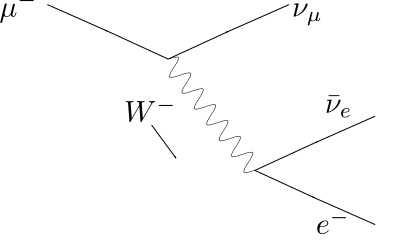
\includegraphics[scale=0.5]{muon_decay}
  \caption{diagrama de Feynman para el decaimiento $\mu^-\to \nu_\mu e^-\bar{\nu}_e$}
  \label{fig:muondecay}
\end{figure}
El propagador para el bos\'on $W$ de momentum $q$ resulta ser
\begin{align}
  \widetilde{D}_{\mu\nu}=\frac{1}{q^2-m_W^2}\left(g_{\mu\nu}-\frac{q_\mu q_\nu}{m_W^2}\right)\,.
\end{align}
Para los prop\'ositos actuales la obtenci\'on de este resultado no es necesaria, el punto importante es que cuando las masas de las part\'\i culas iniciales y finales son mucho m\'as peque\~nas que $m_W$, esto se reduce a
\begin{align}
  \widetilde{D}_{\mu\nu}=-\frac{g_{\mu\nu}}{m_W^2}\,.
\end{align}
Este resultado se entiende f\'acilmente cuando se compara con el propagador de una part\'\i culas escalar masiva $1/(q^2-M^2)\to-1/M^2$. Las componentes espaciales de $W_\mu$ con $\mu=1,2,3$, a bajas energ\'\i as tienen el mismo propagador que el de una part\'\i cula escalar, mientras $W_0$, tiene el signo opuesto.

El Lagrangiano efectivo para el decaimiento del mu\'on, $\mu^-\to \nu_\mu e^- \bar{\nu}_e$ es entonces
\begin{align}
  \mathcal{L}=&\frac{g^2}{8}\left[\bar{\nu}_\mu\gamma^\mu(1-\gamma_5)\mu\right]\frac{g_{\mu\nu}}{m_W^2}
  \left[\bar{e}\gamma^\nu(1-\gamma_5)\nu_e\right]\nonumber\\
=&\frac{g^2}{8m_W^2}\left[\bar{\nu}_\mu\gamma^\mu(1-\gamma_5)\mu\right]
  \left[\bar{e}\gamma^\nu(1-\gamma_5)\nu_e\right]\nonumber\\
  =&\frac{G_F}{\sqrt{2}}\left[\bar{\nu}_\mu\gamma^\mu(1-\gamma_5)\mu\right]\left[\bar{e}\gamma_\mu(1-\gamma_5)\nu_e\right]\,,
\end{align}
donde
\begin{align}
  \frac{G_F}{\sqrt{2}}=&\frac{g^2}{8m_W^2}\nonumber\\
  =&\frac{g^24}{8g^2v^2}\nonumber\\
  =&\frac{1}{2v^2}\,,
\end{align}
y
\begin{align}
  v=\left(\sqrt{2}G_F\right)^{-1/2}\,.
\end{align}


De otro lado, para el  decaimiento $\beta$, $n\to p e^- \bar{\nu}_e$, de acuerdo a la figura~\ref{fig:neutrondecay}, tenemos

\begin{align}
    \mathcal{L}=\frac{G_\beta}{\sqrt{2}}\left[\bar{p}\gamma^\mu(1-1.26\gamma_5)n\right]\left[\bar{e}\gamma_\mu(1-\gamma_5)\nu_e\right]\,.
\end{align}
\begin{figure}
  \centering
  \includegraphics[scale=0.5]{neutrondecay}
  \caption{Decaimiento del neutr\'on.}
  \label{fig:neutrondecay}
\end{figure}
con $G_F$ dado en la ec.~\eqref{eq:233} y $G_\beta=1.10\times10^{-5}\,\text{GeV}^2$. La corriente hadr\'onica tiene la forma V--1.26A. El factor 1.26  puede entenderse como debido a las correcciones a nivel hadr\'onico de una corriente que es de la forma V--A a nivel del quarks, como en la ec.~\eqref{eq:234}. A nivel de quarks el decaimiento del neutr\'on ($udd$) al prot\'on ($uud$) corresponde al decaimiento de uno de los quarks down del neutr\'on $d\to u e^- \bar{\nu}_e$
\begin{align}
    \mathcal{L}=\frac{G_F}{\sqrt{2}}V_{11}\left[\bar{u}\gamma^\mu(1-\gamma_5)d\right]\left[\bar{e}\gamma_\mu(1-\gamma_5)\nu_e\right]\,.
\end{align}
De modo que $G_\beta=G_F V_{11}=G_F\cos\theta_C$, donde $\theta_C$ es el \'angulo de Cabbibo. Una vez se tienen en cuenta correcciones electrod\'ebiles se obtiene el valor $|V_{11}|=0.97418(27)$\cite{PDG}. Las magnitudes de los elementos de la matriz CKM son\cite{PDG}
\begin{align}
  V\approx\begin{pmatrix}
    0.97419&0.2257&0.0359\\
    0.2256&0.97334&0.0415\\
    0.00874&0.0407&0.999133
  \end{pmatrix}\sim \mathbf{1}
\end{align}

\section{C\'alculo de procesos}
\label{sec:calculo-de-procesos}
Se remite al lector al lector a la siguiente parte del curso ``Standard Model and beyond'', de la p\'agina web 

\url{http://gfif.udea.edu.co:2500}

En particular a las secciones iniciales de los Cap\'\i tulos 1 y 2 donde se analizan el decaimiento $W^-\to e^-\bar{\nu}_e$ y el decaimiento del muon. 


\section{Problemas}
\label{sec:problemas-1}
\begin{enumerate}
\item Demuestre expl\'\i citamente la ec.~(\ref{eq:228})
\label{item:chap6.1}
\end{enumerate}


% \left(\right)
%
%%% Local Variables: 
%%% mode: latex
%%% TeX-master: "fullnotes"
%%% End: 

\appendix

\chapter{Soluciones a los problemas}

\section*{Cap\'\i tulo \ref{cha:campos-vectoriales}}

\begin{itemize}
\item[\ref{cha:campos-vectoriales}.\ref{item:pch2.1}.] De
\begin{equation}
  {a'}^\mu=\Lambda^{\mu}_{\ \nu}a^\nu
\end{equation}
tenemos que
\begin{equation}
  {a'}_\rho=g_{\mu\rho}{a'}^\rho=g_{\mu\rho}\Lambda^{\mu}_{\ \nu}g^{\nu\eta}a_\eta=\Lambda^{\ \eta}_{\rho}a_\eta
\end{equation}

De la definici\'on de transformaci\'on de Lorentz
\begin{equation}
  {a'}^{\mu}{b'}_\mu=a^{\mu}b_\mu
\end{equation}
tenemos
\begin{equation}
   {a'}^{\mu}{b'}_\mu=\Lambda^{\mu}_{\ \nu}\Lambda_{\mu}^{\ \rho}a^{\nu}b_\rho=a^\nu b_\nu=\delta^\rho_\nu a^\nu b_\rho
\end{equation}
de donde
\begin{equation}
  \Lambda^{\mu}_{\ \nu}\Lambda_{\mu}^{\ \rho}=\delta^\rho_\nu
\end{equation}

\item[\ref{cha:campos-vectoriales}.\ref{item:pch2.3}.] 
\begin{equation}
  r\sim\frac{1}{m}\approx\frac{1}{80\,\text{GeV}}\times\frac{1\;\text{GeV}}{1/(1.97\times10^{-16}\,\text{m}^{-1})}\approx2.5\times10^{-18}\;\text{m}
\end{equation}

\end{itemize}

\section*{Cap\'\i tulo \ref{cha:princ-gauge-local}}

\begin{itemize}
\item[\ref{cha:princ-gauge-local}.\ref{item:pch3.3}] 
Tenemos  
\begin{equation}
  \tilde\Phi=i\tau_2\Phi^*=\begin{pmatrix}
    0&  1\\
    -1& 0
  \end{pmatrix}
  \begin{pmatrix}
\phi^-\\
{\phi^0}^*    
  \end{pmatrix}=
  \begin{pmatrix}
    {\phi^0}^*\\
    -\phi^-
  \end{pmatrix}
\end{equation}
Haremos la parte correspondiente al t\'ermino de masa. Para el t\'ermino cin\'etico es igual.
\begin{align}
  -m^2\tilde\Phi^\dagger \tilde\Phi
&=-m^2
\begin{pmatrix}
  {\phi^0}&-\phi^+
\end{pmatrix}
\begin{pmatrix}
  {\phi^0}^*\\
  -\phi^-
\end{pmatrix}\nonumber\\
&=-m^2(\phi^0{\phi^0}^*+\phi^+\phi^-)\nonumber\\
&=-m^2\Phi^\dagger \Phi
\end{align}
de modo que $\Phi$ y $\tilde \Phi$ son representaciones equivalentes de $SU(2)$.

Adem\'as
  \begin{align}
   -m^2\epsilon_{ab}\tilde \Phi^a\Phi^b= -m^2(\epsilon_{12}\tilde\Phi^1\Phi^2+\epsilon_{21}\tilde\Phi^2\Phi^1)
    &=-m^2({\phi^0}^*\phi^0+\phi^+\phi^-)\nonumber\\
    &=-m^2\Phi^\dagger \Phi 
  \end{align}
\item[\ref{cha:princ-gauge-local}.\ref{item:pch3.4}] De las ecs.~\eqref{eq:177} y \eqref{eq:178}

   \begin{align}
\mathcal{L}=&
      \partial^\mu{\boldsymbol{\phi}^*}\cdot\partial_\mu\boldsymbol{\phi}-g\left[{\boldsymbol{\phi}^*}\cdot\mathbf{W}_\mu\times\partial^\mu\boldsymbol{\phi}
    -\left(\partial^\mu{\boldsymbol{\phi}^*}\right)\cdot\mathbf{W}_\mu\times\boldsymbol{\phi}\right]
  \nonumber\\
  &+g^2{\phi^*}^i (\delta_{kl}\delta_{im}-\delta_{km}\delta_{il})W^\mu_k W_\mu^l\phi_m-m^2{\boldsymbol{\phi}^*}\cdot \boldsymbol{\phi}-\tfrac{1}{4}W^{\mu\nu}_iW_{\mu\nu}^i\nonumber\\
  =&\partial^\mu{\boldsymbol{\phi}^*}\cdot\partial_\mu\boldsymbol{\phi}-g\left[{\boldsymbol{\phi}^*}\cdot\mathbf{W}_\mu\times\partial^\mu\boldsymbol{\phi}
    -\left(\partial^\mu{\boldsymbol{\phi}^*}\right)\cdot\mathbf{W}_\mu\times\boldsymbol{\phi}\right]
  \nonumber\\
  &+g^2{\phi^*}^i W^\mu_k W_\mu^k\phi_i-g^2{\phi^*}^i W^\mu_k W_\mu^i\phi_k-m^2{\boldsymbol{\phi}^*}\cdot \boldsymbol{\phi}-\tfrac{1}{4}W^{\mu\nu}_iW_{\mu\nu}^i\nonumber\\
  =&\partial^\mu{\boldsymbol{\phi}^*}\cdot\partial_\mu\boldsymbol{\phi}-g\left[{\boldsymbol{\phi}^*}\cdot\mathbf{W}_\mu\times\partial^\mu\boldsymbol{\phi}
    -\left(\partial^\mu{\boldsymbol{\phi}^*}\right)\cdot\mathbf{W}_\mu\times\boldsymbol{\phi}\right]
  \nonumber\\
  &+g^2\boldsymbol{\phi^*}\cdot\boldsymbol{\phi}\mathbf{W}^\mu\cdot \mathbf{W}_\mu-g^2\mathbf{\phi^*}\cdot\mathbf{W}^\mu \mathbf{W}_\mu\cdot\boldsymbol{\phi}-m^2{\boldsymbol{\phi}^*}\cdot  \boldsymbol{\phi}-\tfrac{1}{4}\mathbf{W}^{\mu\nu}\cdot\mathbf{W}_{\mu\nu}
   \end{align}
donde
\begin{align}
     \mathbf{W}^{\mu\nu}\cdot\mathbf{W}_{\mu\nu}=&(\partial^\mu \mathbf{W}^\nu -\partial^\nu \mathbf{W}^\mu)\cdot(\partial_\mu \mathbf{W}_\nu -\partial_\nu \mathbf{W}_\mu)
    +2g(\partial^\mu \mathbf{W}^\nu -\partial^\nu \mathbf{W}^\mu)\cdot \mathbf{W}_\mu\times\mathbf{W}_\nu\nonumber\\
    &+g^2(\delta_{jl}\delta_{km}-\delta_{jm}\delta_{kl})W^\mu_j W^\nu_k W_\mu^l W_\nu^m\nonumber\\
    =&(\partial^\mu \mathbf{W}^\nu -\partial^\nu \mathbf{W}^\mu)\cdot(\partial_\mu \mathbf{W}_\nu -\partial_\nu \mathbf{W}_\mu)
    +2g(\partial^\mu \mathbf{W}^\nu -\partial^\nu \mathbf{W}^\mu)\cdot \mathbf{W}_\mu\times\mathbf{W}_\nu\nonumber\\
    &+g^2(W^\mu_j W^\nu_kW_\mu^j W_\nu^k-W^\mu_j W^\nu_k W_\mu^k W_\nu^j)\nonumber\\
    =&(\partial^\mu \mathbf{W}^\nu -\partial^\nu \mathbf{W}^\mu)\cdot(\partial_\mu \mathbf{W}_\nu -\partial_\nu \mathbf{W}_\mu)
    +2g(\partial^\mu \mathbf{W}^\nu -\partial^\nu \mathbf{W}^\mu)\cdot \mathbf{W}_\mu\times\mathbf{W}_\nu\nonumber\\
    &+g^2(\mathbf{W}^\mu\cdot\mathbf{W}_\mu \mathbf{W}^\nu\cdot\mathbf{W}_\nu-\mathbf{W}^\mu\cdot\mathbf{W}_\nu  \mathbf{W}^\mu \cdot\mathbf{W}_\nu)\nonumber\\
    =&(\partial^\mu \mathbf{W}^\nu -\partial^\nu \mathbf{W}^\mu)\cdot(\partial_\mu \mathbf{W}_\nu -\partial_\nu \mathbf{W}_\mu)
    +2g(\partial^\mu \mathbf{W}^\nu -\partial^\nu \mathbf{W}^\mu)\cdot \mathbf{W}_\mu\times\mathbf{W}_\nu\nonumber\\
    &+g^2(\mathbf{W}^\mu\cdot\mathbf{W}_\mu \mathbf{W}^\nu\cdot\mathbf{W}_\nu-\mathbf{W}^\mu\cdot\mathbf{W}_\nu  \mathbf{W}^\mu \cdot\mathbf{W}_\nu)
\end{align} 

%\item[\ref{cha:princ-gauge-local}.\ref{item:pch3.3}] 
\item[\ref{cha:princ-gauge-local}.\ref{item:pch3.5}]
\begin{equation*}
  \begin{pmatrix}
    W^3_\mu\\
    B_\mu
  \end{pmatrix}=
  \begin{pmatrix}
    \cos\theta_W&\sin\theta_W\\
    -\sin\theta_W&\cos\theta_W
  \end{pmatrix}
  \begin{pmatrix}
    Z_\mu\\
    A_\mu
  \end{pmatrix}\,.
\end{equation*}

\begin{align}
  -\tfrac{1}{4}B^{\mu\nu}B_{\mu\nu}=&-\tfrac{1}{4}(\partial^\mu B^\nu-\partial^\nu B^\mu)(\partial_\mu B_\nu-\partial_\nu B_\mu)\nonumber\\
=&-\tfrac{1}{4}[\partial^\mu (-s Z^\nu+ c A^\nu)-\partial^\nu (-s Z+ c A)^\mu][\partial_\mu (-s Z+ c A)_\nu-\partial_\nu (-s Z+ c A)_\mu]\nonumber\\
=&-\tfrac{1}{4}[-s\partial^\mu Z^\nu +c\partial^\mu A^\nu+s\partial^\nu Z^\mu-c\partial^\nu A^\mu][-s\partial_\mu Z_\nu +c\partial_\mu A_\nu+s\partial_\nu Z_\mu-c\partial_\nu A_\mu]\nonumber\\
=&-\tfrac{1}{4}[-s(\partial^\mu Z^\nu-\partial^\nu Z^\mu)+c(\partial^\mu A^\nu-\partial^\nu A^\mu)][-s(\partial_\mu Z_\nu-\partial_\nu Z_\mu)+c(\partial_\mu A_\nu-\partial_\nu A_\mu)]\nonumber\\
  =&-\tfrac{1}{4}[-s(\partial^\mu Z^\nu-\partial^\nu Z^\mu)+c(\partial^\mu A^\nu-\partial^\nu A^\mu)][-s(\partial_\mu Z_\nu-\partial_\nu Z_\mu)+c(\partial_\mu A_\nu-\partial_\nu A_\mu)]\nonumber\\
=&-\tfrac{1}{4}[s^2(\partial^\mu Z^\nu-\partial^\nu Z^\mu)(\partial_\mu Z_\nu-\partial_\nu Z_\mu)+c^2(\partial^\mu A^\nu-\partial^\nu A^\mu)(\partial_\mu A_\nu-\partial_\nu A_\mu)\nonumber\\
&  -2s c(\partial^\mu Z^\nu-\partial^\nu Z^\mu)(\partial_\mu A_\nu-\partial_\nu A_\mu)]
\end{align}
Similarmente, reemplzando $s^2\leftrightarrow c^2$ y $s\to-s$
\begin{align}
-\tfrac{1}{4}W^{\mu\nu}_3W_{\mu\nu}^3\supset=&-\tfrac{1}{4}[c^2(\partial^\mu Z^\nu-\partial^\nu Z^\mu)(\partial_\mu Z_\nu-\partial_\nu Z_\mu)+s^2(\partial^\mu A^\nu-\partial^\nu A^\mu)(\partial_\mu A_\nu-\partial_\nu A_\mu)\nonumber\\
&  +2s c(\partial^\mu Z^\nu-\partial^\nu Z^\mu)(\partial_\mu A_\nu-\partial_\nu A_\mu)]
\end{align}
\begin{align}
  -\tfrac{1}{4}B^{\mu\nu}B_{\mu\nu}-\tfrac{1}{4}W^{\mu\nu}_3W_{\mu\nu}^3\supset=-\tfrac{1}{4}F^{\mu\nu}F_{\mu\nu}-\tfrac{1}{4}Z^{\mu\nu}Z_{\mu\nu}
\end{align}
De otro lado, teniendo en cuenta que
\begin{align}
  W_\mu^+=&\frac{W_\mu^1-i W_\mu^2}{\sqrt{2}}\nonumber\\
  W_\mu^-=&\frac{W_\mu^1+i W_\mu^2}{\sqrt{2}}\nonumber\\
W_\mu^++W_\mu^-=&\frac{2}{\sqrt{2}}W_\mu^1=\sqrt{2}W_\mu^1\nonumber\\
W_\mu^--W_\mu^+=&\frac{2}{\sqrt{2}}W_\mu^2=\sqrt{2}i W_\mu^2
\end{align}
\begin{align}
  W_\mu^1=&\frac{W_\mu^-+W_\mu^+}{\sqrt{2}}\nonumber\\
  W_\mu^2=&\frac{W_\mu^--W_\mu^+}{\sqrt{2}i}\nonumber\\
\end{align}
\begin{align}
  -\tfrac{1}{4}W^{\mu\nu}_1W_{\mu\nu}^1  -\tfrac{1}{4}W^{\mu\nu}_2W_{\mu\nu}^2\supset&
-\tfrac{1}{4}[(\partial^\mu W^\nu_1-\partial^\nu W^\mu_1)(\partial_\mu W_\nu^1-\partial_\nu W_\mu^1)\nonumber\\
&+(\partial^\mu W^\nu_2-\partial^\nu W^\mu_2)(\partial_\mu W_\nu^2-\partial_\nu W_\mu^2)
]\nonumber\\
 = &-\tfrac{1}{4}\{(\partial^\mu W^\nu_1\partial_\mu W_\nu^1-\partial^\mu W^\nu_1\partial_\nu W_\mu^1-\partial^\nu W^\mu_1\partial_\mu W_\nu^1+\partial^\nu W^\mu_1\partial_\nu W_\mu^1)
\nonumber\\
&+(1\to2)\}\nonumber\\
 = &-\tfrac{1}{4}\{(\partial^\mu W^\nu_1\partial_\mu W_\nu^1-\partial^\mu W^\nu_1\partial_\nu W_\mu^1-\partial^\mu W^\nu_1\partial_\nu W_\mu^1+\partial^\mu W^\nu_1\partial_\mu W_\nu^1)
\nonumber\\
&+(1\to2)\}\nonumber\\
 = &-\tfrac{1}{2}\{(\partial^\mu W^\nu_1\partial_\mu W_\nu^1-\partial^\mu W^\nu_1\partial_\nu W_\mu^1)
+(\partial^\mu W^\nu_2\partial_\mu W_\nu^2-\partial^\mu W^\nu_2\partial_\nu W_\mu^2)
\}\nonumber\\
 = &-\tfrac{1}{4}\{[ (\partial^\mu W^\nu_-+\partial^\mu W^\nu_+)(\partial_\mu W_\nu^-+\partial_\mu W_\nu^+)\nonumber\\
&-(\partial^\mu W^\nu_-+\partial^\mu W^\nu_+)(\partial_\nu W_\mu^-+\partial_\nu W_\mu^+)]\nonumber\\
&+i^2[(\partial^\mu W^\nu_--\partial^\mu W^\nu_+)(\partial_\mu W_\nu^--\partial_\mu W_\nu^+)\nonumber\\
&-(\partial^\mu W^\nu_--\partial^\mu W^\nu_+)(\partial_\nu W_\mu^--\partial_\nu W_\mu^+)]\}\nonumber\\
 = &-\tfrac{1}{4}\{[ (\partial^\mu W^\nu_-+\partial^\mu W^\nu_+)(\partial_\mu W_\nu^-+\partial_\mu W_\nu^+)\nonumber\\
&-(\partial^\mu W^\nu_-+\partial^\mu W^\nu_+)(\partial_\nu W_\mu^-+\partial_\nu W_\mu^+)]\nonumber\\
&-[(\partial^\mu W^\nu_--\partial^\mu W^\nu_+)(\partial_\mu W_\nu^--\partial_\mu W_\nu^+)\nonumber\\
&-(\partial^\mu W^\nu_--\partial^\mu W^\nu_+)(\partial_\nu W_\mu^--\partial_\nu W_\mu^+)]
\}
\end{align}
Teniendo en cuenta que los terminos cruzados son los \'unicos que no se cancelar\'an, tenemos
\begin{align}
 -\tfrac{1}{4}W^{\mu\nu}_1W_{\mu\nu}^1  -\tfrac{1}{4}W^{\mu\nu}_2W_{\mu\nu}^2\supset&
 -\tfrac{1}{2}[ \partial^\mu W^\nu_-\partial_\mu W_\nu^++\partial^\mu W^\nu_+\partial_\mu W_\nu^-
-\partial^\mu W^\nu_-\partial_\nu W_\mu^+-\partial^\mu W^\nu_+\partial_\nu W_\mu^-]\nonumber\\
=& -\tfrac{1}{2}[ \partial^\mu W^\nu_-(\partial_\mu W_\nu^+-\partial_\nu W_\mu^+)+\partial_\mu W_\nu^+\partial^\mu W^\nu_-
-\partial_\mu W_\nu^+\partial^\nu W^\mu_-]\nonumber\\
=& -\tfrac{1}{2}[ \partial^\mu W^\nu_-(\partial_\mu W_\nu^+-\partial_\nu W_\mu^+)+\partial_\nu W_\mu^+\partial^\nu W^\mu_-
-\partial_\mu W_\nu^+\partial^\nu W^\mu_-]\nonumber\\
=& -\tfrac{1}{2}[ \partial^\mu W^\nu_-(\partial_\mu W_\nu^+-\partial_\nu W_\mu^+)
-\partial^\nu W^\mu_-(\partial_\mu W_\nu^+-\partial_\nu W_\mu^+)]\nonumber\\
=& -\tfrac{1}{2}[ (\partial^\mu W^\nu_--\partial^\nu W^\mu_-)(\partial_\mu W_\nu^+-\partial_\nu W_\mu^+)\nonumber\\
=&-\frac{1}{2}(F^\dagger_W)^{\mu\nu}(F_W)_{\mu\nu}\,.
\end{align}


\end{itemize}

\section*{Cap\'\i tulo \ref{cha:modelo-estandar}}

\begin{itemize}
\item[\ref{cha:modelo-estandar}.~\ref{item:chap6.1}.] 
Haciendo un an\'alisis similar al de la secci\'on \ref{sec:invar-gauge-local-1}, tenemos de la ec.~\eqref{eq:125} que
\begin{align}
\mathcal{L}_{fWB}=&i\overline{L}\gamma^\mu\mathcal{D}_\mu L+i\,\overline{e_R}\gamma^\mu\mathcal{D}_\mu e_R  \nonumber\\
=&\begin{pmatrix} 
  i\overline{\nu_L}\gamma^\mu& i\overline{e_L}\gamma^\mu
\end{pmatrix}\begin{pmatrix}
    \partial_\mu-igT_3^\uparrow W^3_\mu-ig'Y_LB_\mu&-\frac{i}{\sqrt{2}}gW^+_\mu\\
    -\frac{i}{\sqrt{2}}gW^-_\mu&\partial_\mu-igT_3^\downarrow W^3_\mu-ig'Y_LB_\mu
  \end{pmatrix}
  \begin{pmatrix}
    \nu_L\\e_L    
  \end{pmatrix}\nonumber\\
&+i\overline{e_R}\gamma^\mu(\partial_\mu-ig'Y_R B_\mu)e_R\nonumber\\
=&\begin{pmatrix} 
  i\overline{\nu_L}\gamma^\mu& i\overline{e_L}\gamma^\mu
\end{pmatrix} 
  \begin{pmatrix}
    (\partial_\mu-igT_3^\uparrow W^3_\mu-ig'Y_LB_\mu)\nu_L-\frac{i}{\sqrt{2}}ge_LW^+_\mu\\
    -\frac{i}{\sqrt{2}}g\nu_LW^-_\mu+(\partial_\mu-igT_3^\downarrow W^3_\mu-ig'Y_LB_\mu)e_L
  \end{pmatrix}+i\overline{e_R}\gamma^\mu(\partial_\mu-ig'Y_R B_\mu)e_R\nonumber\\
=&i\overline{\nu_L}\gamma^\mu(\partial_\mu-igT_3^\nu W^3_\mu-ig'Y_LB_\mu)\nu_L+\frac{1}{\sqrt{2}}g\overline{\nu_L}\gamma^\mu e_LW^+_\mu\nonumber\\
&+\frac{1}{\sqrt{2}}g\overline{e_L}\gamma^\mu\nu_LW^-_\mu+i\overline{e_L}\gamma^\mu(\partial_\mu-igT_3^eW^3_\mu-ig'Y_LB_\mu)e_L
+i\overline{e_R}\gamma^\mu(\partial_\mu-ig'Y_R B_\mu)e_R\nonumber\\
=&i\overline{e_L}\gamma^\mu\partial_\mu e_L+i\overline{e_R}\gamma^\mu\partial_\mu e_R+i\overline{\nu_L}\gamma^\mu\partial_\mu\nu_L
+\frac{1}{\sqrt{2}}g\left(\overline{\nu_L}\gamma^\mu e_LW^+_\mu+\overline{e_L}\gamma^\mu\nu_LW^-_\mu\right)\nonumber\\
&+i\overline{\nu_L}\gamma^\mu(-igT_3^\nu W^3_\mu-ig'Y_LB_\mu)\nu_L+i\overline{e_L}\gamma^\mu(-igT_3^eW^3_\mu-ig'Y_LB_\mu)e_L
+i\overline{e_R}\gamma^\mu(-ig'Y_R B_\mu)e_R
\nonumber\\
=&i\overline{\psi_e}\gamma^\mu\partial_\mu\psi_e+i\overline{\nu_L}\gamma^\mu\partial_\mu\nu_L
+\frac{1}{\sqrt{2}}g\left(\overline{\nu_L}\gamma^\mu e_LW^+_\mu+\text{h.c}\right)+\mathcal{L}_{fAZ}
\end{align}
donde
\begin{align}
\mathcal{L}_{fAZ}=&\overline{\nu_L}\gamma^\mu\nu_L(gT_3^\nu W^3_\mu+g'Y_LB_\mu)+\overline{e_L}\gamma^\mu e_L(gT_3^eW^3_\mu+g'Y_LB_\mu)
+g'\overline{e_R}\gamma^\mu e_R(Y_R B_\mu)
\nonumber\\
=&g\left[\overline{\nu_L}\gamma^\mu\nu_L(T_3^\nu W^3_\mu+\tan\theta_WY_LB_\mu)+\overline{e_L}\gamma^\mu e_L(T_3^eW^3_\mu+\tan\theta_WY_LB_\mu)
+Y_R\tan\theta_W\overline{e_R}\gamma^\mu e_RB_\mu\right]\nonumber\\
=&g\left\{\overline{\nu_L}\gamma^\mu\nu_L[T_3^\nu(\cos\theta_WZ_\mu+\sin\theta_WA_\mu)+\tan\theta_WY_L(-\sin\theta_WZ_\mu+\cos\theta_WA_\mu)]\right.\nonumber\\
&+\overline{e_L}\gamma^\mu e_L[T_3^e(\cos\theta_WZ_\mu+\sin\theta_WA_\mu)+\tan\theta_WY_L(-\sin\theta_WZ_\mu+\cos\theta_WA_\mu)]\nonumber\\
&\left.+Y_R\tan\theta_W\overline{e_R}\gamma^\mu e_R(-\sin\theta_WZ_\mu+\cos\theta_WA_\mu)\right\} 
\nonumber\\
=&\frac{g}{\cos\theta_W}[(T_3^\nu\cos^2\theta_W-Y_L\sin^2\theta_W )\overline{\nu_L}\gamma^\mu\nu_L\nonumber\\
&+(T^e_3\cos^2\theta_W-Y_L\sin^2\theta_W)\overline{e_L}\gamma^\mu e_L+(0\times\cos\theta_W-Y_R\sin^2\theta_W\overline{e_R}\gamma^\mu e_R]Z_\mu\nonumber\\
&+g\sin\theta_W[(T^\nu_3+Y_L)\overline{\nu_L}\gamma^\mu\nu_L+(T_3^e+Y_L)\overline{e_L}\gamma^\mu e_L+(0+Y_R)\overline{e_R}\gamma^\mu e_R]A_\mu.
\end{align}
Como $T_3^f\cos^2\theta_W-Y_f\sin^2\theta_W=T_3-(T_3^f+Y_f)\sin^2\theta_W$, entonces usando $Q_f=T_3^f+Y_f$, y $e=g\sin\theta_W$ tenemos
\begin{equation}
\mathcal{L}_{fAZ}=\sum_{f=e_L,\nu_L,e_R}\left[\frac{e}{\sin\theta_W\cos\theta_W}(T_3^f-Q_f\sin^2\theta_W )Z_\mu+eQ_fA_\mu\right]\overline{f}\gamma^\mu f
\end{equation}
Como $Q_\nu=0$, claramente los neutrinos no se acoplan a los fotones como se esperaba y adem\'as se obtiene la corriente electromagn\'etica apropiada, ya que
\begin{equation}
  \sum_{f=e_L,\nu_L,e_R}eQ_fA_\mu\overline{f}\gamma^\mu f=eQ_e\overline{\psi_e}\gamma^\mu\psi_eA_\mu.
\end{equation}
 
\end{itemize}






%%% Local Variables: 
%%% mode: latex
%%% TeX-master: "fullnotes"
%%% End: 

%use 
% $ latexbiblio2itex file.tex 
% to generate instiki file
%instiki:category: FisicaSubatomica
%instiki:
%instiki:# Bibliograf\'\i a #
%instiki:
%instiki:***
%instiki:
%instiki:[[NotasFS|Tabla de Contenidos]]
%instiki:
%instiki:***

\begin{thebibliography}{999}
\bibitem{kane} 
Modern Elementary Particle Physics, Gordon Kane, Perseus Publishing, 1993.

\bibitem{cottingham}
An Introduction to Standard Model of Particle Physics. W.N Cottingham and D.A. Greenwood, Cambridge University Press, 1988

\bibitem{r}
Quantum Field Theory, L.H Reyder, Cambridge University Press

\bibitem{q}
Quantum Field Theory, F. Mandl, G. Shaw, John Wiley \& Sons, INC. 1993

\bibitem{a} 
A. Pich, The Standard Model of Electroweak Interactions, hep-ph/0502010

\bibitem{aa} 
The Standard Model: Alchemy and Astrology, hep-ph/0609274

\bibitem{ultimo} 
Relativistic Quantum Mechanics and Field Theory, Franz Gross, John Wiley \& Sons, INC. 1993

\bibitem{ActionPhysics} 
\url{http://es.wikipedia.org/wiki/Principio_de_m\%C3\%ADnima_acci\%C3\%B3n}, 
\url{http://en.wikipedia.org/wiki/Action_\%28physics\%29}


\bibitem{JavaAP}\url{http://www.eftaylor.com/software/ActionApplets/LeastAction.html}

\bibitem{NewtonSeconLaw} 
\url{http://es.wikipedia.org/wiki/Leyes_de_Newton#Segunda_Ley_de_Newton_o_Ley_de_la_Fuerza}, 
\href{http://en.wikipedia.org/wiki/Newton\%27s_laws_of_motion#Newton.27s_second_law:_law_of_acceleration}{http://en.wikipedia.org/wiki/Newton\%27s\_laws\_of\_motion}

\bibitem{Gross}
Relativistic Quantum Mechanics and Field Theory, Franz Gross, Wiley Interscience, 1993, Chapter 1.

\bibitem{Gauss}
\url{http://es.wikipedia.org/wiki/Teorema_de_la_divergencia}

\bibitem{daelembertiano}
\url{http://en.wikipedia.org/wiki/D%27Alembertian}

\bibitem{Goldhaber:1971mr}
  A.~S.~Goldhaber and M.~M.~Nieto,
  ``Terrestrial and extra-terrestrial limits on the photon mass,''
  Rev.\ Mod.\ Phys.\  {\bf 43} (1971) 277.

\bibitem{Yao:2006px}
  W.~M.~Yao {\it et al.}  [Particle Data Group],
  ``Review of particle physics,''
  J.\ Phys.\ G {\bf 33}, 1 (2006).

\bibitem{Pauli}
\url{http://en.wikipedia.org/wiki/Pauli_matrices}

\bibitem{Englert:1964et}
  F.~Englert and R.~Brout,
  ``Broken Symmetry and the Mass of Gauge Vector Mesons,''
  Phys.\ Rev.\ Lett.\  {\bf 13} (1964) 321.
  %%CITATION = PRLTA,13,321;%%
  %2524 citations counted in INSPIRE as of 25 Jul 2014

\bibitem{Higgs:1964pj}
  P.~W.~Higgs,
  ``BROKEN SYMMETRIES AND THE MASSES OF GAUGE BOSONS,''
  Phys.\ Rev.\ Lett.\  {\bf 13} (1964) 508.
  P.~W.~Higgs,
  ``Spontaneous Symmetry Breakdown Without Massless Bosons,''
  Phys.\ Rev.\  {\bf 145} (1966) 1156.


\bibitem{Pich:2005mk}
  A.~Pich,
  ``The standard model of electroweak interactions,''
  arXiv:hep-ph/0502010,
  Published in *Sant Feliu de Guixols 2004, European School of High-Energy Physics* 1-48.

\bibitem{NU}
\url{http://en.wikipedia.org/wiki/Natural_units}
\bibitem{PU}
\url{http://en.wikipedia.org/wiki/Plank_units}

\bibitem{Aitchison:2003tq}
  I.~J.~R.~Aitchison and A.~J.~G.~Hey,
  ``Gauge theories in particle physics: A practical introduction. Vol. 1: From
  relativistic quantum mechanics to QED,''
%\href{http://www.slac.stanford.edu/spires/find/hep/www?irn=5562635}{SPIRES entry}
{\it  Bristol, UK: IOP (2003) 406 p}

\bibitem{andim}
\url{http://groups.google.com/group/sci.physics.research/msg/e6cc1b288df8bbb2}

\bibitem{PDG} 
 W.~M.~Yao {\it et al.}  [Particle Data Group],
  ``Review of particle physics,''
  J.\ Phys.\ G {\bf 33} (2006) 1.

\bibitem{Ryder:1985wq}
  L.~H.~Ryder,
  ``Quantum Field Theory,''
{\it  Cambridge, Uk: Univ. Pr. ( 1985) 443p}
%\href{http://www.slac.stanford.edu/spires/find/hep/www?irn=1444956}{SPIRES entry}

\bibitem{GN} 
\url{http://en.wikipedia.org/wiki/Gell-Mann–Nishijima_formula}

\bibitem{spin}
\url{http://en.wikipedia.org/wiki/Spin_(physics)}

\bibitem{LEP}
\url{http://en.wikipedia.org/wiki/LEP}

\bibitem{muon}
\url{http://en.wikipedia.org/wiki/Muon}

\bibitem{uslhcblog}\url{http://blogs.uslhc.us/?p=481}

\bibitem{Veltman} Lie Groups in Physics, M.J.G Veltman (English version by G. 't Hooft)

\bibitem{Brading:2000hc}
  K.~Brading and H.~R.~Brown,
  ``Noether's theorems and gauge symmetries,''
  hep-th/0009058.


\bibitem{Brading:2003nv}
  K.~Brading and E.~Castellani,
  ``Symmetries in physics: Philosophical reflections,''
  Cambridge, UK: Univ. Pr. (2003) 445 p

\bibitem{Sundermeyer:2014kha}
  K.~Sundermeyer,
  ``Symmetries in fundamental physics,''
  Fundam.\ Theor.\ Phys.\  {\bf 176} (2014).
  doi:10.1007/978-94-007-7642-5

\bibitem{Noehter} Emmy~Noether,Invariant variation problems, arXiv:physics/0503066.


\end{thebibliography}
%%% Local Variables: 
%%% mode: latex
%%% TeX-master: "fullnotes"
%%% End:

\end{document}


%%% Local Variables: 
%%% mode: latex
%%% TeX-master: "fullnotes"
%%% End: 
